\documentclass[12pt,a4paper]{thesis}
\usepackage[utf8]{inputenc}
\usepackage[T1]{fontenc}
\usepackage[main=french]{babel}
\usepackage{caption} % For making "french" tables & figures

\usepackage[top=90pt, bottom=90pt, left=80pt, right=80pt]{geometry}			% Geometrie de la page
\usepackage{fancyhdr} % Header/Footer
\usepackage{changepage} % Local margins adjusting %adjustwidth

\usepackage{lmodern} % ou toute autre fonte complète pour le français : kpfonts, fourier...
\usepackage{xspace} % pour profiter du mécanisme
\usepackage[np]{numprint} % si je dois écrire des nombres sans unités sinon
% \usepackage{siunitx} % si je dois écrire des grandeurs avec unités
\usepackage{booktabs}
\usepackage{csquotes}
\usepackage{imakeidx}
\usepackage[bottom]{footmisc} % always place footer at bottom of page

\usepackage{minitoc} % Table of Contents local to a chapter
\mtcselectlanguage{french} % Minitoc en francais

\frenchbsetup{og=«,fg=»} % define pour guillemets français

\usepackage{lipsum} % For Lorem Ipsum generation : \lipsum or \lipsum[2-4] paragraphes 2 a 4
\usepackage{datetime} % pour \currenttime (affiche l'heure)

\usepackage{amsmath}
\usepackage{amsfonts}
\usepackage{amssymb}
\usepackage{ulem} % \sout pour barrer du texte

\usepackage{graphicx}
\usepackage{enumitem}
\usepackage{multirow}
\usepackage{nicematrix} % Better arrays (for aligning cline content on multirows)

\newcolumntype{P}[1]{>{\raggedright\arraybackslash }m{#1}}

\usepackage{array}
\newcolumntype{R}[1]{>{\raggedleft\arraybackslash }b{#1}}
\newcolumntype{L}[1]{>{\raggedright\arraybackslash }b{#1}}
\newcolumntype{C}[1]{>{\centering\arraybackslash }b{#1}}

\newcolumntype{M}[1]{>{\raggedright\let\newline\\\arraybackslash\hspace{0pt}}m{#1}} % another L
\newcolumntype{D}[1]{>{\centering\let\newline\\\arraybackslash\hspace{0pt}}m{#1}}   % another C
\newcolumntype{S}[1]{>{\raggedleft\let\newline\\\arraybackslash\hspace{0pt}}m{#1}}  % another R


\usepackage{color}
\definecolor{heavy-blue}{RGB}{0,0,150}
%\definecolor{Gray}{gray}{0.9}
%\definecolor{LightCyan}{rgb}{0.88,1,1}
%\definecolor{olivine}{rgb}{0.6, 0.73, 0.45} % Vert clair
%\definecolor{lightgreen}{rgb}{0.56, 0.93, 0.56}
%\definecolor{lightcoral}{rgb}{0.94, 0.5, 0.5} % Rouge clair


\newcolumntype{"}{@{\hskip\tabcolsep\vrule width 1pt\hskip\tabcolsep}} %%%% colonne " pour "bold" dans tableau


\newcommand{\thickcline}[1]{%            %%%% Definit \thickhcline pour faire cline{x-y} "bold" dans tableau
    \@thickcline #1\@nil%
}

\def\@thickcline#1-#2\@nil{%
  \omit
  \@multicnt#1%
  \advance\@multispan\m@ne
  \ifnum\@multicnt=\@ne\@firstofone{&\omit}\fi
  \@multicnt#2%
  \advance\@multicnt-#1%
  \advance\@multispan\@ne
  \leaders\hrule\@height1pt\hfill
  \cr
  \noalign{\vskip-1pt}%
}


\usepackage[pdftitle={CREA : Méthode d'analyse, d'adaptation et de réutilisation des processus à forte intensité de connaissances},
	pdfsubject={CREA : Méthode d'analyse, d'adaptation et de réutilisation des processus à forte intensité de connaissances - cas d'utilisation dans l'enseignement supérieur en informatique},
	pdfauthor={Fabrice BOISSIER},
	pdfkeywords={Processus à forte intensité de connaissances; Adaptive case management; Gestion de cas; Réutilisation de connaissances; Extraction de connaissances; Analyse de concepts formels; Traitement automatique du langage; Numérisation de l'enseignement; Enseignement}]{hyperref}
\hypersetup{
	colorlinks=true,
	linktoc=section,
	linkcolor=heavy-blue,
	citecolor=heavy-blue,
	filecolor=red,
	urlcolor=blue
}

\usepackage{lastpage}

% \TTBF (texte)
%% Texte en ttfamily + textbf (TeleType + Bold Font)
\newcommand{\TTBF}[1]{\texttt{\textbf{#1}}}

% Command up ! Pour 20e siecle
%\newcommand{\up}[1]{\textsuperscript{#1}}

% correct bad hyphenation here
\hyphenation{op-tical net-works semi-conduc-tor PyCATSHOO}

\pagestyle{empty}

\newenvironment{vcenterpage}
{\newpage\vspace*{\fill}}
{\vspace*{\fill}\par\pagebreak}

%%%%%%%%%%%%%%%%%%%%%%%
%% Header
%%%%%%%%%%%%%%%%%%%%%%%
%\lhead{\texttt{\chaptername~\thechapter}}			%Gauche Haut
%\chead{}											%Centre Haut
%\rhead{}											%Droite Haut
%\lfoot{}											%Gauche Bas
%\cfoot{\thepage}									%Centre Bas
%\rfoot{}											%Droite Bas


\fancypagestyle{IHA-fancy-style}{%
  \fancyhf{}% Clear header and footer
  %\fancyhead[LE,RO]{\slshape \rightmark}
  %\fancyhead[LO,RE]{\slshape \leftmark}
  %\fancyhead[LE,RO]{Blabla} % Gauche page paire, Droite page impaire
  %\fancyhead[LO,RE]{Blob} % Droite page paire, Gauche page impaire
  %\fancyhead[L]{\texttt{\chaptername~\thechapter}}
  \fancyhead[L]{\texttt{\leftmark}} % \chaptermark crashes in fancyheader, use \leftmark instead
  \fancyfoot[C]{\thepage\ / \pageref*{LastPage}} % Custom footer  % pagref : link   pageref* : no link
  \renewcommand{\headrulewidth}{0.4pt}% Line at the header visible
  \renewcommand{\footrulewidth}{0.4pt}% Line at the footer visible
}

\fancypagestyle{plain}{%
  \fancyhf{}%
  \fancyfoot[C]{\thepage\ / \pageref{LastPage}}%
  \renewcommand{\headrulewidth}{0pt}% Line at the header invisible
  \renewcommand{\footrulewidth}{0.4pt}% Line at the footer visible
}

%----------------------------------------------------------------------------------------
%   FOOTER FOOTNOTE PATCH  % Linked with usepackage[bottom]{footmisc}
%----------------------------------------------------------------------------------------
%
\let\origfootrule\footrule
\renewcommand{\footrule}{\iffootnote{}{\origfootrule}}
\renewcommand\footnoterule{\origfootrule}
%%%%%%% END FOOTER FOOTNOTE PATCH

%%%%%%%%%%%%%%%%%%%%%%%%%%%%%%%%%%%%%%%
%% Caracteristiques de la Page Titre %%
%%%%%%%%%%%%%%%%%%%%%%%%%%%%%%%%%%%%%%%
\makeatletter
\def\maketitle{
	\begin{titlepage}

	\newgeometry{top=1cm,bottom=1cm,left=2cm,right=2cm}

	\begin{center}
	%%% LOGO PARIS 1 %%%
	
\includegraphics[scale=0.4]{logos/logo_coul_fr_cmjn.jpg}
	\null\vskip 0.1cm%\vfill

	\MakeUppercase{Thèse de Doctorat} \\
	\MakeUppercase{de l'Université Paris 1 Panthéon - Sorbonne}
	\null\vskip 0.3cm%\vfill
	Préparée au sein du Centre de Recherche en Informatique (EA 1445)\\
	à L'École Doctorale de Management Panthéon - Sorbonne (ED 559)
	\null\vskip 0.8cm%\vfill

	Présentée par : \\
	\null\vskip 0.1cm%\vfill
	{\Large \textbf{\MakeUppercase{Fabrice BOISSIER}} }
	\null\vskip 0.8cm%\vfill

	Pour l'obtention du grade de Docteur de L'Université Paris 1 Panthéon - Sorbonne \\
	\null\vskip 0.8cm%\vfill

	{\LARGE \textbf{\@title}}\\
	\bigskip
	{\Large \textbf{\textit{\@subtitle}}}

	\null\vskip 0.3cm%\vfill
	Spécialité : Informatique
	\null\vskip 0.5cm%\vfill
	Thèse présentée et soutenue publiquement à Paris, le 17 janvier 2022 \\
	%\null\vskip 0.5cm%\vfill
	Composition du jury :
	\end{center}

	\begin{adjustwidth}{-60pt}{-60pt} % Enlarge the margins only here {left}{right}  // OK : -50pt  -50pt
	\begin{center}
	%%\begin{table}[ht]
	%%\centering
	%%\resizebox{\textwidth}{!}{
	{ \footnotesize
	\begin{tabular}{l m{6.5cm} l}   %%% Comme il n'y aura que 4 membres externes du jury, l'espacement passera : & & \\ {l m{6cm} l}
	\multirow{2}{*}{M. Guillaume CLEUZIOU} & Professeur, & \multirow{2}{*}{Rapporteur} \\
	 & Université d'Orléans &  \\ % Professeur des Universités
%	 & & \\
	\multirow{2}{*}{M. Alain WEGMANN} & Professeur, & \multirow{2}{*}{Rapporteur} \\
	 & École Polytechnique Fédérale de Lausanne &  \\ % Professeur Ordinaire
	 & & \\
	\multirow{2}{*}{Mme. Daniela GRIGORI} & Professeur, & \multirow{2}{*}{Examinatrice} \\
	 & Université Paris Dauphine - PSL &  \\ % Professeur des Universités
%	 & & \\
	\multirow{2}{*}{M. Camille SALINESI} & Professeur, & \multirow{2}{*}{Examinateur} \\
	 & Université Paris 1 Panthéon - Sorbonne &  \\ % Professeur des Universités
	 & & \\
	\multirow{2}{*}{Mme. Bénédicte LE GRAND} & Professeur, & \multirow{2}{*}{Directrice de Thèse} \\
	 & Université Paris 1 Panthéon - Sorbonne &  \\ % Professeur des Universités
%	 & & \\
	\multirow{2}{*}{Mme. Irina RYCHKOVA} & Maître de Conférence, & \multirow{2}{*}{Co-Encadrante de Thèse} \\
	 & Université Paris 1 Panthéon - Sorbonne &  \\ % Maître de Conférence
	\end{tabular}
	}
	%%\end{table}
	\end{center}
	\end{adjustwidth}

	\begin{center}
	\null\vskip 0.8cm%\vfill
	%{ \scriptsize Version du \today ~ (\currenttime) }
	\end{center}

	\restoregeometry

	\end{titlepage}
}


%\newcommand{\up}[1]{\textsuperscript{#1}} %Definition de UP !

%%%%%%%%%%%%%%%%%%%%%%%%%%%%%%%%%%%%%%%%%%%%%%%%%%%%%%%%%%%%%%%%%%%%%%%%%%%%%%%
%% INFORMATIONS VARIEES                                                      %%
%%                                                                           %%
%% Traduction des termes :                                                   %%
%% Knowledge Intensive Process: Processus à Forte Intensité de Connaissances %%
%% Knowledge Worker: Travailleur du Savoir (travailleur de la connaissance ?)%%
%%                                                                           %%
%%%%%%%%%%%%%%%%%%%%%%%%%%%%%%%%%%%%%%%%%%%%%%%%%%%%%%%%%%%%%%%%%%%%%%%%%%%%%%%

\newcommand{\MyCREA}{Case REuse and Adaptation}

%%%%%%%%%%%%%%%%



\begin{document} % Problem with \author requires to begin document before \author

\dominitoc % Initialization of minitoc / ToC local to chapters

%------------------------------------------------------------------------------
%	TITLE SECTION
%------------------------------------------------------------------------------

\title{CREA : Méthode d'analyse, d'adaptation et de réutilisation des processus à forte intensité de connaissances}

\subtitle{cas d'utilisation dans l'enseignement supérieur en informatique}

\author{Fabrice BOISSIER}

\date{17 Janvier 2022}

%------------------------------------------------------------------------------

%\begin{document}
\maketitle

%\thispagestyle{empty}
%%% FOR ALL INTRODUCTION PAGE STYLE EMPTY
\pagestyle{empty}

\newpage
%%% GEOMETRY AND OTHERS ARE BROKEN BY THE SPECIAL TITLE
\restoregeometry

~\newpage % Seconde page vierge / 2e de couverture

%------------------------------------------------
\pagestyle{IHA-fancy-style}

% Remerciements
\begin{center}
\begin{LARGE}
Remerciements
\end{LARGE}
\end{center}

\bigskip

%%%%%%%%%%%%%

\begin{small}

Je remercie tout d'abord mes encadrantes, Bénédicte Le Grand et Irina Rychkova de m'avoir encadré et accompagné pour cette thèse pendant laquelle beaucoup trop d'évènements imprévus se sont produits (mais au moins, on peut littéralement appeler ça l'aventure de la thèse !).
Beaucoup de chemins, détours, impasses, raccourcis, ... ont été explorés, pour finalement construire cette carte.
Ce fut complexe, long, parfois très laborieux, mais nous y sommes arrivés.
Lorsque j'ai lu pour la première fois l'intitulé du sujet (\og \textit{Exploration des higraphs et de l'analyse formelle de concepts pour la modélisation des processus métier à forte intensité de connaissance et pour l'évaluation des modèles} \fg), je ne voyais absolument pas où commençait et finissait chaque terme... mais je suis aujourd'hui ravi de pouvoir expliquer plusieurs d'entre eux !
Même chose sur les méthodologies de recherche : design science, action research, behavior, et bien d'autres qu'il me reste à découvrir.
Je ne pensais absolument pas toucher à autant de domaines en démarrant une thèse en informatique, mais je suis comblé par toutes ces connaissances (et je souhaite réellement continuer à apprendre et comprendre).
Merci encore Bénédicte et Irina !

\smallskip

Je tiens également à remercier les rapporteurs qui ont accepté de relire mon manuscrit : Alain Wegmann et Guillaume Cleuziou.
Leurs précieux conseils et remarques m'ont effectivement aidé à développer ce qu'il manquait, et j'espère pouvoir continuer à creuser certaines de leurs pistes dans de futurs travaux.
Je remercie aussi Daniela Grigori et Camille Salinesi d'avoir accepté les rôles d'examinateurs.

\smallskip

Merci énormément au CRI et à l'ensemble de ses membres pour l'ensemble de vos avis critiques et les interminables discussions.
Une pensée émue et pleine de souvenirs à Ali Jaffal, Elena Viorica Epure, Elena Kushnareva, Nourhène Ben Rabah, Afef Awadid, Danillo Sprovieri, Asmaa Achtaich : merci pour vos soutiens.
Une pensée moins émue et beaucoup plus actuelle à David Beserra, Floriane Owczarek, Angela Patricia Villota Gomez, Luisa Fernanda Rincon, Sabrine Edded, Houssem Chemingui, et aux tous derniers (qui vont y arriver) : Nicolas Six, Claudia Negri, Ramona Elally, Camilo Correa.
Sans oublier les collègues : Stéphane, Emmanuelle, Corinne, Astrid, Diem, Gabriel, Sarah, Julien, et Brigitte.
Et les anciens camarades de classe : Gözde Kiraç, Nassima Mazouz, Wassila Bey Zekkoub.

\smallskip

Je n'oublie pas les membres du LSE à EPITA pour m'avoir accueilli sur la fin de cette thèse : Marc Espie (les maths, OpenBSD, ... je continue d'apprendre grâce à toi !), Robert Erra (les métriques : nous allons les traiter), Mark Angousturès (on ne lâche pas le data science, ni la recherche), Reda Dehak, Alizée Pénel, Laurent \& Loïca (bip !), et Alexandre Letois.

%\medskip
\smallskip

Plus largement, je remercie \textit{infiniment} l'ensemble des enseignantes et enseignants qui m'ont fait adorer les études et les diverses matières qui existent.
C'est-à-dire, les professeurs des écoles en maternelle et en primaire, les professeurs des collèges et lycées, les professeurs et enseignants[-chercheurs] titulaires ou non à l'EPITA, à l'UQAC, et évidemment à l'Université Paris 1 Panthéon - Sorbonne.
Je garderai éternellement d'excellents souvenirs de vous toutes et tous :
% Maternelle
Laurence, Cécile,
% Primaire
André Ménini, Maria Raison, \'Elisabeth Aubin,
% 6e (Collège)
M\up{me} Croué (même si c'était difficile de retenir toutes les définitions par c\oe{}ur), M\up{me} Oeuvrard, M\up{me} Corbic,
% 5e
M. Brassard, Bernard Roquejoffre, M\up{me} Gautry,
% 4e
Gaston Époté Myke, M. Huchon, Peggy Sultan, M\up{me} Mouchez, M\up{me} Lorgeril,
% 3e
M\up{me} Le Texier, M\up{me} Luccioni, M. Azam, M. Tobaty,
% 2nde (Lycée)
M. Nefati,
% 1ere S
Michel Volkovitch (et ses fabuleuses phrases à traduire concernant les flûtes et les synthétiseurs), M. Garcia, M. Oucif (Pierre Loti, \og Vers Ispahan \fg, \og Aziyadé \fg), M. Begis (pour sa patience infinie),
% Terminale S
M\up{me} Staszak (surtout le tout dernier cours de philosophie le 6 juin 2006), M\up{me} Ehanno,
% EPITA - Prépa
Nathalie "Junior" Bouquet, Christophe "Krisboul" Boullay, Christelle Trémoulet, Anne-Sophie Dujardin, Olivier Rodot, Marwan Burelle, mes ACD Nicolas Ballas (ballas\_n) et Mathieu Sabarly (sabarl\_m),
% EPITA - Ing1
Didier Verna, Akim Demaille, Thierry Géraud, % \LaTeX passe pas avec Verna T.T
% EPITA - SRS
Sébastien Bombal, \'Eric Gaillard, Aurélien Borde, Julien Sterckeman,
% UQAC
M. Bouchard,
% Paris 1
Samira Si-said Cherfi, Saïd Assar, Fayçal Hamdi, Camille Salinesi, Rébecca Deneckère, Irina Rychkova, Bénédicte Le Grand.

Cette thèse a beau être la somme des travaux d'une équipe de chercheurs, sans vous toutes et tous pour m'enseigner autant de choses, je n'aurais jamais acquis assez de connaissances pour mener à bien ce projet de recherche.
Une pensée également pour André Rossano qui m'a particulièrement touché lorsqu'il nous expliquait le mainframe, et ses anecdotes de travail d'une autre ère sur S/370 et l'ASR 33.

%% 1988 - 1989
%% 1989 - 1990
%% 1990 - 1991
%% 1991 - 1992 : Petite Section Maternelle (Jean-François, Laurence)
%% 1992 - 1993 : Moyenne Section Maternelle (Cécile)
%% 1993 - 1994 : Grande Section Maternelle (Catherine, Brigitte)
%% 1994 - 1995 : CP (André Ménini)
%% 1995 - 1996 : CE1 (André Ménini)
%% 1996 - 1997 : CE2 (Maria Raison)
%% 1997 - 1998 : CM1 (Odile ???)
%% 1998 - 1999 : CM2 (Elisabeth Aubin, Madame Debune)
%% 1999 - 2000 : 6e3 (anglais : Mme Pastor, maths : Mme Croué, français : Mme Oeuvrard, histoire/geo : Mme Gallo, svt : Mme Corbic, techno : Mme Dubucq, musique : Mme Fleury, arts plastiques : M ???, EPS : Mme Le Strat)
%% 2000 - 2001 : 5e1 (français : Mme Moumaneix, maths : M Quillivic, histoire/geo : Mme Felip, anglais : Mme Fiévet, svt : Mme Giraudeau, physique/chimie : M Durand / M Garcin, techno : Mme Gautry, musique : M Brassard, arts plastiques : Bernard Roquejoffre, EPS : Mme Le Strat, Latin : M Uda)
%% 2001 - 2002 : 4e5 (physique/chimie : Gaston Epoté Myke, maths : Mme Lorgeril, français : Mme Mouchez, histoire/geo : M Huchon, anglais : Mme Peggy Sultan, svt : Mme , techno : M Marniche, espagnol : Mme Gérinard, musique : xxx, arts plastiques : Mme Trouillard, EPS : Mme "STGEPS" ! Mme Fauvet)
%% 2002 - 2003 : 3e3 (français : Mme Luccioni, maths : Mme Le Texier, histoire/geo : M Tobaty/M Mériau, anglais : Mme Brugerolle, svt : Mme Corbic, physique/chimie : Mme Lorans, techno : M Azam (fabrice), espagnol : Mme Rodriguez, musique : xxx, arts plastiques : Bernard Roquejoffre)
%% 2003 - 2004 : Seconde 4 ~ (physique/chimie : M Nefati (Heddi Neffati ?), Histoire/Géo : Mme Gernigon, svt : Mme Fereira, maths : Mme Graff, français : Mme Gallier, anglais : Mme Bondarenco, espagnol : Mme Vecchini, MPI : Mme Ehanno, EPS : M Vergniol, LCE : Mme Boutin)
%% 2004 - 2005 : Premiere S 4 (svt : Mme Brelet (Anne Brelet ?), Physique/Chimie : M Nefati (Heddi Neffati ?), maths : Mme Filippi, français : Georges Oucif, histoire/geo : M Garcia, anglais : Michel Volkovitch, espagnol : Mme Pays && M Achouchi, EPS : M Begis, LCE : Mme Hadida)
%% 2005 - 2006 : Terminale S 2 (svt : M Vasseur, Physique/Chimie : Mme Ehanno, maths normale : Mme Hubert, maths spécialité : Mme Vallaud, philosophie : Mme Staszak, histoire/geo : M Lucas, anglais : Mme Petit, espagnol : Mme Souche, EPS : M Begis, LCE : M Gille)
%% 2006 - 2007 : InfoSup A2 (ACD : ballas_n Ballas Nicolas & sabarl_m Sabarly Mathieu)
%% 2007 - 2008 : InfoSpe A1
%% 2008 - 2009 : InfoSpe A1
%% 2009 - 2010 : Ing1 Groupe B
%% 2010 - 2011 : Ing2 SRS (Sébastien Bomabal SSI - Aurélien Borde WSEC - Julien Sterckeman Sécu - Jean-François Lubrano AD - Eric Gaillard Réseau)
%% 2011 - 2012 : Ing3 SRS (André Rossano Formateur IBM depuis OS/370)
%% 2012 - 2013 : Aubay (Travail)
%% 2013 - 2014 : Aubay (Travail)
%% 2014 - 2015 : Master SID (Paris 1)
%% 2015 - 2016 : (Paris 1, recherche libre Architecture d'Entreprise & Décentralisation)
%% 2016 - 2017 : Doctorat 1ère année (Contrat Doctoral - Paris 1) : Statechart, HiGraph, & KiP
%% 2017 - 2018 : Doctorat 2e année (Contrat Doctoral - Paris 1) : Ontologies, BPM, EPC
%% 2018 - 2019 : Doctorat 3e année (Contrat Doctoral - Paris 1) : BPM, KIP  ==> Sujet OK ! (+ Passage au BAIP & SCUIO)
%% 2019 - 2020 : Doctorat 4e année (demi-ATER - Paris 1) : BPM, KIP, ACF, TAL/NLP, Règles d'Association, Clustering
%% 2020 - 2021 : Doctorat 5e année (demi-ATER - Paris 1) : BPM, KIP, ACF, TAL/NLP, Clustering
%% 2021 - 2022 : Fin Doctorat (Paris 1 && Enseignant-Chercheur EPITA au LSE)
%%


%\medskip
\smallskip

Je pense également à vous toutes et tous... Jason Brillante en premier pour absolument tout, y compris les moments au Liberty Rock Studio gravés à jamais dans nos c\oe{}urs et mémoires.
Éva Debray pour ses conseils, relectures, encouragements, appels, jus de citrons, explications, remises en question de mes certitudes, ...
Si j'ai appris les méthodes de recherche en informatique au labo, j'ai appris beaucoup de choses sur la philosophie, le contrôle social, Spinoza, les sciences de l'éducation, l'histoire de l'école en France, ... grâce à toi, tes explications, et tes corrections.
Merci Éva.
Soutiens indéfectibles depuis plus de 10 ans maintenant (merci de me remonter le moral) : Geoffrey Tan, Laurent Garcin, Shanand Seeram, Jérémy Meng, Riyad Yakine.
Merci à Kathleen Ripert pour le soutien un peu trop lointain depuis l'Allemagne... mais le soutien est là, et c'est le plus important ! (Tu reviens quand à Paris ?)
Une pensée particulière à Ghislain Guillot (oui, tu comptes beaucoup quand même).

\smallskip

Je remercie toutes et tous les amis et potes du monde entier (GameSeries, Red-Network, Dimension MMX, D.Folk, ...) : Merlin, Vadim, Diana, Renan, Rémi, Frédéric, Justin, Christian, Marion, Jean-Baptiste, Lisa, Guillaume, Sophie, Éléonore, Samantha, Angélina, Johanna, Clara, Marine, Sarah, Elisa, Axel, Stacy, Alex(andra), Axel, Julie, Lionel, Patricia, ... sans oublier Robert Rafie et les épi-potes ! (Raph', Cédric, Pierre, Justin, Fabien, Cyril, Alexandre, Aurélie, Gabriel, Lucas, François, Alban, Florent, Robin, Joe, Nils, ...)

%\medskip
\smallskip

Alexandre Abraham, Lydie Gustafsson, et Egle Tomasi m'ont permis de sauter le pas et réellement faire une thèse : ce manuscrit n'existerait pas sans vous, ni mon changement radical de carrière.

\smallskip

Grâce aux doctorantes et doctorants de Paris 1 (parfois avec le doctorat) et d'ailleurs, j'ai découvert les SHS.
Et sans vous, je serais encore un nigaud qui dirait des bêtises sur vos domaines : Hélène Bénistand, Léon Guillot, Armand Desprairies, Guillaume Noblet, Orianne Tercerie, Juliette Fontaine, Bastien Rueff, Cécile Bourgade, Maëlle de Seze, Milan Bonté, Hugo Vidon, Justine Audebrand, Anaïs Bonano, Sahra Rausch, Karim Abou-Merhi, Evélia Mayenga, Marine Lassery, Matthieu Febvre-Issaly, Typhaine Rahault, Guillemette Prevot, Michaël Pierrelée, Nicolas Jouvin, Clément, ...
Et merci aux étudiantes et étudiants qui m'ont beaucoup appris ou avec qui j'ai bien ri : Joachim "Jojo" Loysel, Sami, Émilie, Thib', Hasna, Lucas, Maximilien, Trystan, Emilio, Jo, Marie, Elsa, Lorenz, Jaspal, Ulysse, Adèle, Diu, Nurlan, ...

Plus généralement, je remercie tou·te·s les camarades de Mobdoc et autres organisations.
Vivement le 27 Nivôse (Zinc) de l'an CCXXX (230) !

%\medskip
\smallskip

Je n'oublie pas les plus importants : mes parents (Robert Boissier et Patricia Kissling), mes grands-parents (Willy, Augusta, Rosa), tous les autres membres (Yvette, Frédérique, Bertrand, Isabelle, Tiffany, Ornella, Robin, ...).
Sans ma mère, je ne sais pas si j'aurais eu le bac (et je rigolerais probablement moins).
Sans mon père, je ne sais pas si j'aurais fait de l'informatique (et je m'intéresserais probablement à beaucoup moins de choses).

\end{small}


\newpage

\pagestyle{IHA-fancy-style}

% Abstract/Résumé
\begin{center}
\begin{LARGE}
Résumé
\end{LARGE}

\bigskip

\textbf{\@title}

\textbf{\textit{\@subtitle}}

\end{center}

\bigskip

%%%%%%%%%%%%%


La crise sanitaire du COVID-19 a particulièrement accéléré le mouvement de numérisation pourtant déjà initié depuis quelques décennies dans l'enseignement supérieur.
De nombreuses activités ont dû être adaptées dans l'urgence, tout particulièrement les réunions entre enseignants, l'évaluation des étudiants et les enseignements.
Ces activités sont des exemples de processus \og \textit{à forte intensité de connaissances} \fg (ou \og \textit{knowledge intensive processes} \fg en anglais) qui partagent des caractéristiques rendant difficile l'intégration du numérique, telles que :
\begin{itemize}
\item l'abondance de connaissances mobilisables, autant de la part des étudiants lors de leurs travaux que de la part des enseignants évaluant ou adaptant leurs cours,
\item la collaboration entre toutes les parties prenantes du monde de l'enseignement supérieur,
\item la créativité requise pour s'adapter au contexte incertain.
\end{itemize}
Ce besoin rapide de déployer de nouveaux processus à forte intensité de connaissances, ou d'adapter ceux qui existent, se confronte à de nombreux défis connus de ce domaine de recherche spécifique.
La question est de savoir comment réutiliser des connaissances existantes, par exemple des connaissances entreposées en ligne dont l'abondance rend difficile la sélection des plus adaptées aux besoins des enseignants.

Dans cette thèse, nous proposons la méthode CREA réutilisant des cas passés dans le domaine de l'enseignement supérieur, en particulier pour la construction de cours.
La méthode CREA permet de réutiliser des supports de cours existants pour tout d'abord représenter visuellement l'écart entre eux, mais également de proposer des séances de cours présentées sous forme de regroupements de sujets majeurs à aborder.
D'autres types de documents peuvent également être intégrés parmi les supports de cours (des pages webs, ou des articles de recherche), afin de proposer des regroupements adaptés à un public particulier, voire de proposer des regroupements à l'état de l'art de la recherche.
Cette méthode s'appuie sur des outils de traitement automatique de la langue pour extraire les termes employés indépendamment de la langue d'origine, puis sur l'analyse de concepts formels pour calculer des métriques permettant de construire des regroupements de termes et évaluer la similarité des cours fournis en entrée.
Nous proposons également des résultats préliminaires d'une méthode d'ordonnancement des séances.


%%%%%%%%%%%%%

\bigskip

\textbf{Mots clés :
Processus à forte intensité de connaissances,
Adaptive case management,
Gestion de cas,
Réutilisation de connaissances,
Extraction de connaissances,
Analyse de concepts formels,
Traitement automatique du langage,
Numérisation de l'enseignement,
Enseignement}

%%%%%%%%%%%%%%%%%%%%%%%%%%%%%%%%%%%%%%%%%%%%%%%%%%%%%%%%%%%%%%%%%

\newpage

%%%%%%%%%%%%%%%%%%%%%%%%%%%%%%%%%%%%%%%%%%%%%%%%%%%%%%%%%%%%%%%%%

\shorthandoff{:} % REMOVE SPACE BEFORE SEMICOLON

\begin{center}
\begin{LARGE}
Abstract
\end{LARGE}

\bigskip

%CREA : Méthode d’analyse, d’adaptation et de réutilisation des instances de processus à forte intensité de connaissances
%\textbf{\@title}
\textbf{CREA: Method for knowledge intensive process analysis, adaptation and reuse}

% cas d’utilisation dans l’enseignement supérieur en informatique
%\textbf{\textit{\@subtitle}}
\textbf{\textit{use case in postgraduate computer science studies}}

\end{center}

\bigskip

%%%%%%%%%%%%%


Similarly to business domains, digitalisation and virtualisation of processes in higher education started a few decades ago.
During COVID-19 pandemics, the interest in solutions for developing and delivering classes on-line grew substantially.
Nevertheless, solutions allowing for efficient adaptation and reuse of the existing courses and teaching materials in the new circumstances are still lagging.
Transformation of a traditional course to a virtual one, developing a new course adapted for the audience are some examples of  " \textit{knowledge intensive processes} ".
These processes share common properties making digitalization hard, to cite some:
\begin{itemize}
\item they depend on the extensive knowledge and experience of teachers analysing the context and adapting class accordingly,
\item they involve an intense collaboration between all stakeholders in the higher education environment,
\item they require creativity for adapting to uncertain context.
\end{itemize}
Deploying new knowledge intensive processes, or adapting existing ones in this unexpected situation, faced multiple challenges already known from this specific research domain.
The main issue is: how to best reuse existing knowledge, including online stored knowledge, where the abundance of sources and data makes it difficult to select the most suited to teachers' requirements.

In this thesis we propose the CREA method that enables a reuse of past cases in the higher education domain, particularly in courses preparation.
The CREA method supports the reuse of existing courses materials: (i) it presents graphically the gap (i.e. semantic difference) between the courses and (ii) it summarises the class sessions in a form of clusters of main terms to discuss.
Other types of documents can also be integrated within the input courses materials (including web pages, or research articles) in order to propose adapted clusters for specific audiences, or even state-of-the-art materials.
This method relies on natural language processing tools in order to extract the terms regardless of the input language, then it uses formal concept analysis for computing metrics to build clusters of terms and assess the similarity of input materials.
We also propose some preliminary results of a session scheduling method.


%%%%%%%%%%%%%

\bigskip

\textbf{Keywords:
Knowledge intensive process,
Adaptive case management,
Case Management,
Knowledge Reuse,
Knowledge Extraction,
Formal concept analysis,
Natural language processing,
Digitalisation of education,
Education}

\shorthandon{:} % RE-ACTIVATE SPACE BEFORE A SEMICOLON


%------------------------------------------------

\newpage

%% KEEP TABLE OF CONTENTS WITHOUT STYLE
\pagestyle{empty}
\addtocontents{toc}{\protect\thispagestyle{empty}}

\tableofcontents

\clearpage

\listoffigures
\listoftables

%% REWRITE ONLY NOW THE FANCY-HEADER STYLE
\cleardoublepage

\pagestyle{IHA-fancy-style}

% Introduction
\chapter{Introduction}
\label{chapter:Introduction}

Dans ce chapitre, nous introduisons le sujet de cette thèse en expliquant succinctement les processus à forte intensité de connaissances, puis leurs concrétisations dans le contexte du domaine de l'enseignement supérieur, en particulier dans le cas de la construction d'un cours et de la réutilisation des connaissances.
La problématique de recherche est ensuite détaillée ainsi que les hypothèses et stratégies de validation.


\bigskip

\minitoc % Creating an actual minitoc / ToC local to a chapter

\newpage

\section{Contexte sociétal : l'enseignement supérieur et la réutilisation des connaissances}
\label{section:Introduction:ContexteSocietal}

Le numérique un peu plus présent chaque jour, nous montre simultanément les nombreuses opportunités pour accroître notre confort et notre productivité, mais également les limites rencontrées face à certains traits humains encore difficiles à mesurer par des machines et leurs capteurs (les subtilités des jeux de mots et de l'humour, par exemple).
Ces limites se retrouvent dans de nombreux aspects des métiers, y compris dans la gestion des processus qui a pourtant su profiter de l'automatisation croissante~\cite{weske2007business}.
La gestion des processus métier modélise traditionnellement les tâches et activités, ainsi que leur ordonnancement, afin de décrire \textit{comment} réaliser un processus~\cite{kushnareva2016modelingFromGoalsToScenarios}.
Cependant, des caractéristiques liées au contexte ou à l'expertise des différents participants sont difficilement capturées et représentées dans les modèles existants, rendant certains processus peu répétables en l'état.
Ces processus en particulier ont été étudiés et font l'objet d'un champ de recherche supplémentaire dans la gestion et les systèmes d'informations : les \textit{processus à forte intensité de connaissances}, ou \textit{knowledge intensive processes} (KIP) en anglais.
Les processus à forte intensité de connaissances sont caractérisés~\cite{di2015knowledge} par : la manipulation de connaissances (implicites ou explicites), la collaboration entre participants au processus, l'imprédictibilité du contexte et de l'ordre des activités (voire l'apparition d'activités inconnues lors de la conception du processus), l'émergence d'informations au fur et à mesure qui influent sur la décision des activités à exécuter, l'apparition de buts intermédiaires à atteindre pour mener à bien le processus, la prise en charge d'évènements parfois imprévisibles, le respect de règles et contraintes limitant les activités possibles, et enfin, la non-répétabilité due aux situations uniques.

\bigskip

Les processus à forte intensité de connaissances se retrouvent dans de nombreuses activités où l'usage de connaissances dans un contexte collaboratif prédomine : une réunion, par exemple, est annoncée avec un ordre du jour, mais celui-ci ne sera pas toujours respecté, voire, des points seront ajoutés à cause d'évènements inattendus se produisant entre temps ou parce que des participants auront partagé des informations importantes.
Les processus à forte intensité de connaissances peuvent parfois se rapprocher des processus classiques (prévisibles, détaillés, et dont les états sont connus à l'avance), par exemple lors de la résolution de problèmes connus et récurrents, ou au contraire s'en éloigner totalement lorsqu'une très forte exigence de créativité est nécessaire, comme dans les productions artistiques par exemple.
Il existe plusieurs points de vue permettant de mieux apprécier le parcours entre plusieurs activités.
En utilisant deux points de vue sur le suivi d'un patient dans un parcours médical, on se rend compte qu'un hôpital est bel et bien géré par des processus parfaitement prévisibles, mais le patient venant en consultation ne sait pas du tout à l'avance s'il sera hospitalisé ni quels tests il devra effectuer.
Par exemple, effectuer une radiographie s'exécute avec des techniciens de santé précis en respectant une procédure bien définie, mais le personnel de santé ne sait pas à l'avance quels tests seront nécessaires pour chaque patient.
Cette distinction entre les points de vue \textit{processus} (la structure, l'ordre, et la connaissance en amont des activités à effectuer) et \textit{cas} (chaque instance de processus évolue différemment des autres, et dépend des personnes impliquées) illustre comment le contexte et les participants influencent le déroulement des activités.
Là où l'hôpital gère des équipes et des machines selon des procédures précises, tout en devant s'adapter aux évènements survenant dans la société (en 2020 et 2021, il est plus probable de voir arriver des patients en détresse respiratoire, par exemple), le patient sera au contraire vu comme un cas évoluant au fur et à mesure des tests et résultats afin de l'orienter vers les spécialistes adaptés et lui fournir le traitement spécifique à sa situation.

\bigskip

Les caractéristiques des processus à forte intensité de connaissances soulèvent plusieurs défis concernant la gestion du flux de connaissances manipulées, l'aspect collaboratif et les décisions dépendant du contexte, l'intégration du contexte à la conception, la conformité des processus et de leurs instances, la flexibilité requise par les utilisateurs, et enfin, la réutilisation de fragments de processus~\cite{boissier2019challenges}.
Ce dernier défi est au croisement des deux points de vue \textit{cas} et \textit{processus} car il vise à réutiliser les résultats des instances passées de processus (assimilables à des cas terminés et validés) pour aider les utilisateurs à exécuter de nouvelles instances et construire de nouveaux processus (tous les deux assimilables à de nouveaux cas).

\bigskip

Dans le contexte de l'enseignement supérieur, l'intégration du numérique s'effectue depuis une quinzaine d'années grâce aux \textit{innovations pédagogiques numériques} (IPN)~\cite{dulbecco2018innovations}.
Les IPN ont permis de transformer en outils en ligne de nombreux processus administratifs utilisant auparavant des données sur support papier, personnaliser les parcours de formation en les rendant plus flexibles, mais aussi soutenir le développement de nouvelles solutions pédagogiques s'appuyant sur le numérique~\cite{dulbecco2019experimentation}.
Comme dans toutes les organisations, intégrer complètement ou partiellement les processus à forte intensité de connaissances aux systèmes informatiques est beaucoup plus difficile que pour les processus plus classiques : la crise du COVID-19 a montré que le déploiement massif de solutions de visio-conférences est certes un soutien technique supplémentaire, mais pas une prise en charge complète de l'activité d'enseignement.
La construction d'un cours, ou sa reconstruction lors du changement de l'enseignant responsable, est typiquement une activité impliquant d'analyser précisément le contexte dans lequel le cours doit être donné (niveau de la filière/du diplôme, autres cours dépendants des connaissances transmises aux étudiants, cours précédemment suivis par les étudiants, ...) afin de sélectionner les informations précises à transmettre parmi celles existantes dans le domaine.
Un enseignant développant un nouveau cours, ou devant reprendre un cours existant en se l'appropriant et en le mettant à jour, doit donc s'assurer de la pertinence des sources utilisées pour le contexte qu'il vise, et sélectionner des parties réutilisables pour former un support de cours à jour, compréhensible, et utile aux étudiants.

\bigskip

Cette thèse présente nos travaux visant à extraire des connaissances issues de cas passés, évaluer leur pertinence, et proposer à un utilisateur de les réutiliser dans un format organisé.
Pour cela, nous avons choisi le domaine de l'enseignement supérieur et de la recherche, et plus spécifiquement le cas d'un enseignant cherchant à construire un cours sur plusieurs séances à partir de supports de cours existants, et éventuellement en y ajoutant des articles de recherche traitant du même sujet.
L'étude d'un domaine de recherche nécessite de maintenir une connaissance des questions et défis actuellement posés, auxquelles les contributions tentent de répondre, tout en collaborant avec l'ensemble de la communauté.
Une grande créativité est donc requise pour poser des hypothèses et concevoir des contributions permettant de les confirmer ou infirmer.
Lorsqu'un domaine devient suffisamment mature grâce à une somme conséquente de contributions, une diffusion de ces connaissances au-delà des experts peut se réaliser au travers de monographies ou de cours de spécialisation pour former de nouveaux experts.
La préparation d'un cours constitue donc une synthèse des connaissances connues et vérifiées, afin de la transmettre à des personnes potentiellement peu voire non-initiées.
Nous n'aborderons pas la façon de transmettre ces connaissances (représentant la gestion du flux de connaissances), ceci appartenant au domaine de la science de l'éducation, mais nous nous pencherons sur la façon d'extraire ces connaissances des documents existants afin d'évaluer leur pertinence vis-à-vis d'un sujet en particulier (prise en compte du contexte) et proposer une réorganisation de ces connaissances sous forme de séances de cours (réutilisation de fragments d'instances passées).



%%%%%%%%%%%%%%%%%%%%%%%%%%%%%%%%%%%%%%%%%%%%%%%%%%%%%%%%%%%%%%%%%%%%%%%%%%%%%%%%%%%%%%%%%%
%%%%%%%%%%%%%%%%%%%%%%%%%%%%%%%%%%%%%%%%%%%%%%%%%%%%%%%%%%%%%%%%%%%%%%%%%%%%%%%%%%%%%%%%%%
%%%%%%%%%%%%%%%%%%%%%%%%%%%%%%%%%%%%%%%%%%%%%%%%%%%%%%%%%%%%%%%%%%%%%%%%%%%%%%%%%%%%%%%%%%
%%%%%%%%%%%%%%%%%%%%%%%%%%%%%%%%%%%%%%%%%%%%%%%%%%%%%%%%%%%%%%%%%%%%%%%%%%%%%%%%%%%%%%%%%%
%%%%%%%%%%%%%%%%%%%%%%%%%%%%%%%%%%%%%%%%%%%%%%%%%%%%%%%%%%%%%%%%%%%%%%%%%%%%%%%%%%%%%%%%%%
%%%%%%%%%%%%%%%%%%%%%%%%%%%%%%%%%%%%%%%%%%%%%%%%%%%%%%%%%%%%%%%%%%%%%%%%%%%%%%%%%%%%%%%%%%

%%%%%%%%%%%%%%%%%%%%%%%%%%%%%%%%%%%%%%%%%%%%
\clearpage % Clean for pictures and tables %
\newpage   % Clean for pictures and tables %
%%%%%%%%%%%%%%%%%%%%%%%%%%%%%%%%%%%%%%%%%%%%

%%%%%%%%%%%%%%%%%%%%%%%%%%%%%%%%%%%%%%%%%%%%%%%%%%%%%%%%%%%%%%%%%%%%%%%%%%%%%%%%%%%%%%%%%%
%%%%%%%%%%%%%%%%%%%%%%%%%%%%%%%%%%%%%%%%%%%%%%%%%%%%%%%%%%%%%%%%%%%%%%%%%%%%%%%%%%%%%%%%%%
%%%%%%%%%%%%%%%%%%%%%%%%%%%%%%%%%%%%%%%%%%%%%%%%%%%%%%%%%%%%%%%%%%%%%%%%%%%%%%%%%%%%%%%%%%
%%%%%%%%%%%%%%%%%%%%%%%%%%%%%%%%%%%%%%%%%%%%%%%%%%%%%%%%%%%%%%%%%%%%%%%%%%%%%%%%%%%%%%%%%%
%%%%%%%%%%%%%%%%%%%%%%%%%%%%%%%%%%%%%%%%%%%%%%%%%%%%%%%%%%%%%%%%%%%%%%%%%%%%%%%%%%%%%%%%%%
%%%%%%%%%%%%%%%%%%%%%%%%%%%%%%%%%%%%%%%%%%%%%%%%%%%%%%%%%%%%%%%%%%%%%%%%%%%%%%%%%%%%%%%%%%


\section{Problématique de recherche}
\label{section:Introduction:ProblematiqueRecherche}

Les diverses crises récemment rencontrées ont mis en évidence les limites des outils mis à disposition, et plus largement les difficultés à intégrer les processus à forte intensité de connaissances aux systèmes informatiques.
D'après la littérature~\cite{boissier2019challenges} plusieurs défis restent à relever, en particulier celui de la réutilisation de fragments de processus.
Plusieurs travaux ont étudié ces défis et ont proposé des contributions s'adressant à plusieurs domaines d'application.
%%%%
Les fragments de processus~\cite{eberle2009process}\cite{eberle2010process} sont étudiés dans quelques travaux soit en s'intéressant au \textit{raisonnement à base de cas}~\cite{slade1991case}, ou \textit{Case-Based Reasoning} (CBR) en anglais, qui réutilise explicitement les cas passés~\cite{cognini2016case}, soit en reconstituant un modèle de processus avec des contraintes d'exécution locales à chaque activité~\cite{di2013mining}.
Enfin, certains travaux~\cite{zasada2018box} génèrent des \textit{motifs} (ou \textit{patterns} en anglais) à partir de textes légaux afin de s'assurer du respect de la réglementation dans l'industrie alimentaire.
Cette méthode s'appuie sur la rigidité des règles de rédaction des documents réglementaires pour en extraire des motifs, et exploite les expressions régulières pour s'assurer de leur respect.

\bigskip

Dans le cadre de l'enseignement supérieur et de la recherche, nous nous intéressons en particulier au processus de création de cours, et particulièrement à l'aide à la construction de cours à partir de supports existants.
La préparation d'un cours exige beaucoup de temps, y compris lors de sa mise à jour pour inclure des nouveautés ou avec les dernières avancées de la recherche académique.
Les récents évènements nous montrant également qu'il est parfois nécessaire de modifier rapidement les contenus pour s'adapter, nous proposons une méthode permettant d'utiliser des documents texte afin de mesurer leur cohérence vis-à-vis d'un sujet donné et d'en extraire une structure de séances réutilisable.
La proposition de cette thèse vise donc à aider les enseignants à mieux gérer certains de leurs processus à forte intensité de connaissances, en particulier ceux impliqués dans le cadre de la construction d'un cours.
Nos travaux visent donc à répondre à la question de recherche suivante :

%\smallskip
\bigskip

\textbf{Comment aider un enseignant à construire un cours à partir de documents existants, et en s'appuyant sur la réutilisation de connaissances ?}

%\smallskip
\bigskip

Cette question vise donc deux défis posés par les processus à forte intensité de connaissances : la réutilisation de fragments pour former des nouveaux cours, et la prise en compte du contexte au travers de la vérification de la pertinence des documents.
Pour répondre à cette question et aux défis associés, nous posons plusieurs sous-questions de recherche et hypothèses :

\bigskip

\centerline{
\begin{tabular}{c p{12cm}}
1.a & Comment définir le contexte d'un cours ? \\
\end{tabular}
}

\centerline{
%\begin{tabular}{| C{0.75cm} | p{7cm} | p{6cm} |}
\begin{NiceTabular}{| C{0.75cm} | P{7cm} | P{6cm} |}
\hline
H1 & Le contexte d'un cours est défini par les documents sélectionnés
& Comparer plusieurs corpus documentaires: certains homogènes sur un seul sujet, d'autres contenant plusieurs sujets \textit{[Voir scénarios n°1-2-3-4-5]} \\
\hline
\end{NiceTabular}
%\end{tabular}
}

\bigskip

\centerline{
\begin{tabular}{c p{12cm}}
1.b & Comment extraire les termes pertinents par rapport au contexte ? \\
\end{tabular}
}

\centerline{
\begin{NiceTabular}{| C{0.75cm} | P{7cm} | P{6cm} |}
\hline
H2 & Des techniques de TAL permettent d'analyser les documents et d'extraire les termes pertinents
& Vérifier les termes retenus par les outils de TAL une fois leurs analyses terminées, le tout sur plusieurs sujets distincts  \textit{[Voir scénarios n°1-2-3-5]} \\
\hline
\end{NiceTabular}
}

%%%%%%%%%%%%%%%%%%%%%%%%%%%%%%%%%%%%%%%%%%%%%%%%%%%%%%%%%%%%%%%%%%%%%%
%%%%%%%%%%%%%%%%%%%%%%%%%%%%%%%%%%%%%%%%%%%%%%%%%%%%%%%%%%%%%%%%%%%%%%
\bigskip

\vspace{0.5cm}

\centerline{
\begin{tabular}{c p{12cm}}
2 & Comment s'assurer de la pertinence des documents sélectionnés dans le contexte visé et des termes extraits ? \\
\end{tabular}
}

\centerline{
\begin{NiceTabular}{| C{0.75cm} | P{7cm} | P{6cm} |}
\hline
H3 & L'analyse du graphe d'impact mutuel permet d'évaluer la pertinence des sous-ensembles de documents et d'identifier les écarts entre les documents
& Comparer plusieurs corpus documentaires: des corpus homogènes sur un seul sujet doivent montrer un ensemble de documents très rapprochés ou tous aussi éloignés les uns des autres, d'autres corpus contenant plusieurs sujets doivent montrer que des documents sont plus éloignés du sujet central traité par la majorité des documents \textit{[Voir scénarios n°1-2-3-4-5]} \\
\hline
\end{NiceTabular}
}

%%%%%%%%%%%%%%%%%%%%%%%%%%%%%%%%%%%%%%%%%%%%%%%%%%%%%%%%%%%%%%%%%%%%%%
%%%%%%%%%%%%%%%%%%%%%%%%%%%%%%%%%%%%%%%%%%%%%%%%%%%%%%%%%%%%%%%%%%%%%%
\bigskip

\vspace{0.5cm}

\centerline{
\begin{tabular}{c p{12cm}}
3.a & Quelles connaissances tacites sont présentes dans les documents étudiés ? \\
\end{tabular}
}

\centerline{
\begin{NiceTabular}{| C{0.75cm} | P{7cm} | P{6cm} |}
\hline
H4 & Étant donné que la rédaction de supports de cours est une activité humaine avec un objectif de transmission de connaissances sur un sujet, considérons que les connaissances tacites suivantes peuvent être extraites d'un tel support :
& \Block{4-1}{Expliciter les liens en regroupant les termes liés et évaluer la qualité de ces regroupements, expliciter l'ordre des  regroupements et évaluer la qualité de ces regroupements \textit{[Voir scénarios n°1-3-5]}} \\
\cline{1-2}
H4a & Sélection de termes particuliers pour un contexte particulier visé (et non l'ensemble du champs lexical possible)
 & \\
\cline{1-2}
H4b & Organisation de termes sous forme de groupes logiques (séquence, section, chapitre, ...) pour traiter un aspect particulier à la fois
 & \\
\cline{1-2}
H4c & Présentation de thèmes au fur et à mesure selon un ordre précis (permettant d'assurer que les pré-requis soient abordés en premier)
 & \\
\hline
\end{NiceTabular}
}

%%%%%%%%%%%%%%%%%%%%%%%%%%%%%%%%%%%%%%%%%%%%%%%%%%%%%%%%%%%%%%%%%%%%%%
%%%%%%%%%%%%%%%%%%%%%%%%%%%%%%%%%%%%%%%%%%%%%%%%%%%%%%%%%%%%%%%%%%%%%%
%\bigskip

%\vspace{0.5cm}

%%%%%%%%%% =====> just for a better output
\newpage

\vspace*{\fill}

\centerline{
\begin{tabular}{c p{12cm}}
3.b & Comment extraire les connaissances tacites présentes dans les documents étudiés ? \\
\end{tabular}
}

\centerline{
\begin{NiceTabular}{| C{0.75cm} | P{7cm} | P{6cm} |}
\hline
H5 & La similarité conceptuelle permet l'extraction de connaissances tacites, en particulier les regroupements logiques de termes traitant d'un ou quelques aspects particuliers d'un sujet
& Construire des regroupements de termes en utilisant la similarité conceptuelle, et évaluer ces regroupements \textit{[Voir scénarios n°1-3-5]} \\
\hline
\end{NiceTabular}
}

%%%%%%%%%%%%%%%%%%%%%%%%%%%%%%%%%%%%%%%%%%%%%%%%%%%%%%%%%%%%%%%%%%%%%%
%%%%%%%%%%%%%%%%%%%%%%%%%%%%%%%%%%%%%%%%%%%%%%%%%%%%%%%%%%%%%%%%%%%%%%
\bigskip

%\vspace{0.5cm}
% ===> ESTHETIQUE
\vspace*{\fill}

\centerline{
\begin{tabular}{c p{12cm}}
4 & Comment la sélection initiale des documents peut-elle impacter les résultats d'application de la méthode CREA ? \\
\end{tabular}
}

\centerline{
\begin{NiceTabular}{| C{0.75cm} | P{7cm} | P{6cm} |}
\hline
H6 & Les résultats d'application de la méthode CREA sont exploitables par les enseignants et ne sont pas impactés par :
& \Block{4-1}{Tester plusieurs scénarios dont les sujets, langues, et nombre de documents varient \textit{[Voir scénarios n°1-3-5]}} \\
\cline{1-2}
H6a & Le choix initial du sujet de cours
& \\
\cline{1-2}
H6b & Le nombre de document initialement sélectionnés
& \\
\cline{1-2}
H6c & La langue des documents sélectionnés
& \\
\hline
\end{NiceTabular}
}


\centerline{
\begin{NiceTabular}{| C{0.75cm} | P{7cm} | P{6cm} |}
\hline
H7 & Les résultats d'application de la méthode CREA peuvent être impactés par :
& \Block{3-1}{Tester la méthode avec des documents hétérogènes et des contenus diversifiés afin d'évaluer la qualité des résultats \textit{[Voir scénarios n°2-4-5]}} \\
\cline{1-2}
H7a & La présence de documents hétérogènes dans la sélection initiale (articles de recherches, supports de cours, livres,...)
& \\
\cline{1-2}
H7b & La présence de parties (section, chapitre, ...) hors sujet au sein d'un document
& \\
\cline{1-2}
H7c & La nature du contenu des documents (images, listings du code, ...)
& \\
\hline
\end{NiceTabular}
}

\vspace*{\fill}

%%%%%%%%%%%%%%%%%%%%%%%%%%%%%%%%%%%%%%%%%%%%%%%%%%%%%%%%%%%%%%%%%%%%%%
%%%%%%%%%%%%%%%%%%%%%%%%%%%%%%%%%%%%%%%%%%%%%%%%%%%%%%%%%%%%%%%%%%%%%%
%\bigskip
%%%%%%%%%% =====> just for a better output
\newpage

\vspace{0.5cm}

\centerline{
\begin{tabular}{c p{12cm}}
5 & Comment présenter les résultats de la méthode CREA afin d'améliorer l'exploitabilité pour un enseignant ? \\
\end{tabular}
}

\centerline{
\begin{NiceTabular}{| C{0.75cm} | P{7cm} | P{6cm} |}
\hline
H8 & Le graphe d'impact mutuel permet d'aider un enseignant en rendant certaines informations plus visuelles :
& \Block{4-1}{Comparer plusieurs corpus documentaires: des corpus homogènes sur un seul sujet doivent montrer un ensemble de documents très rapprochés ou tous aussi éloignés les uns des autres, d'autres corpus contenant plusieurs sujets doivent montrer que des documents sont plus éloignés du sujet central traité par la majorité des documents  \textit{[Voir scénarios n°1-2-3-4-5]}} \\
\cline{1-2}
H8a & Le graphe d'impact mutuel permet de visualiser le contexte traité par le corpus documentaire
& \\
\cline{1-2}
H8b & Le graphe d'impact mutuel permet de visualiser l'écart de chaque document par rapport au contexte (cf H3)
& \\
\cline{1-2}
H8c & Le graphe d'impact mutuel n'est pas une représentation suffisante pour visualiser avec le maximum de précision les écarts entre documents
& \\
\hline
\end{NiceTabular}
}

\centerline{
\begin{NiceTabular}{| C{0.75cm} | P{7cm} | P{6cm} |}
\hline
H9 & La présentation de clusters de termes sous la forme de tableaux impose implicitement l'ordre de lecture
& Utiliser des méthodes de visualisation de données (nuage de mots, ...) \textit{[Non traité/Voir discussions et conclusion]} \\
\hline
\end{NiceTabular}
}

\bigskip

%%%
Les travaux précédemment cités se concentrent soit sur des domaines trop éloignés (industrie alimentaire), soit sur des processus trop structurés où les tâches sont au c\oe{}ur d'un modèle, soit n'exploitent pas assez la sémantique des textes et des connaissances contenues.
Des travaux existants~\cite{tang2016interactive} se sont intéressés à l'extraction de connaissances et leur analyse avec des techniques mathématiques d'analyse de données, en particulier avec l'\textit{analyse de concepts formels}, ou \textit{formal concept analysis} (FCA) en anglais.
Notre contribution, la méthode CREA (\textit{\MyCREA}), y adjoint des métriques et visualisations issues de l'analyse de concepts formels étudiées dans d'autres travaux~\cite{jaffal2019aide} afin de pouvoir valider la réutilisation de fragments de processus et la vérification de la pertinence.
Plusieurs scénarios d'utilisation sont possibles : construire un tout nouveau cours à partir de supports existants (des documents sont rassemblés et une structure de cours est proposée), mettre à jour son propre cours en le comparant avec les supports d'autres cours (une carte indique l'éloignement de son cours par rapport aux autres), voire en l'étoffant avec des notions issues d'articles de recherche du monde académique (des articles de recherche sont ajoutés à la base de documents insérés afin de proposer une structure plus étendue encore).

\bigskip

Nous avons également commencé à étudier l'aspect temporel en proposant succinctement parmi les perspectives un ordonnancement pour les séances générées.
Les documents dont l'organisation est chronologique permettent d'en extraire non seulement des connaissances, mais également l'ordre de présentation de ces connaissances.
L'ordonnancement temporel a déjà été étudié dans certains travaux~\cite{di2013mining}.
Nous présentons cependant des résultats préliminaires d'une version adaptée à l'organisation temporelle de clusters de notions.
Une extension à la contribution principale et une expérience sont présentées en conclusion pour ordonnancer partiellement les clusters précédemment générés.


%%%%%%%%%%%%%%%%%%%%%%%%%%%%%%%%%%%%%%%%%%%%%%%%%%%%%%%%%%%%%%%%%%%%%%%%%%%%%%%%%%%%%%%%%%
%%%%%%%%%%%%%%%%%%%%%%%%%%%%%%%%%%%%%%%%%%%%%%%%%%%%%%%%%%%%%%%%%%%%%%%%%%%%%%%%%%%%%%%%%%
%%%%%%%%%%%%%%%%%%%%%%%%%%%%%%%%%%%%%%%%%%%%%%%%%%%%%%%%%%%%%%%%%%%%%%%%%%%%%%%%%%%%%%%%%%
%%%%%%%%%%%%%%%%%%%%%%%%%%%%%%%%%%%%%%%%%%%%%%%%%%%%%%%%%%%%%%%%%%%%%%%%%%%%%%%%%%%%%%%%%%
%%%%%%%%%%%%%%%%%%%%%%%%%%%%%%%%%%%%%%%%%%%%%%%%%%%%%%%%%%%%%%%%%%%%%%%%%%%%%%%%%%%%%%%%%%
%%%%%%%%%%%%%%%%%%%%%%%%%%%%%%%%%%%%%%%%%%%%%%%%%%%%%%%%%%%%%%%%%%%%%%%%%%%%%%%%%%%%%%%%%%

%%%%%%%%%%%%%%%%%%%%%%%%%%%%%%%%%%%%%%%%%%%%
\clearpage % Clean for pictures and tables %
\newpage   % Clean for pictures and tables %
%%%%%%%%%%%%%%%%%%%%%%%%%%%%%%%%%%%%%%%%%%%%

%%%%%%%%%%%%%%%%%%%%%%%%%%%%%%%%%%%%%%%%%%%%%%%%%%%%%%%%%%%%%%%%%%%%%%%%%%%%%%%%%%%%%%%%%%
%%%%%%%%%%%%%%%%%%%%%%%%%%%%%%%%%%%%%%%%%%%%%%%%%%%%%%%%%%%%%%%%%%%%%%%%%%%%%%%%%%%%%%%%%%
%%%%%%%%%%%%%%%%%%%%%%%%%%%%%%%%%%%%%%%%%%%%%%%%%%%%%%%%%%%%%%%%%%%%%%%%%%%%%%%%%%%%%%%%%%
%%%%%%%%%%%%%%%%%%%%%%%%%%%%%%%%%%%%%%%%%%%%%%%%%%%%%%%%%%%%%%%%%%%%%%%%%%%%%%%%%%%%%%%%%%
%%%%%%%%%%%%%%%%%%%%%%%%%%%%%%%%%%%%%%%%%%%%%%%%%%%%%%%%%%%%%%%%%%%%%%%%%%%%%%%%%%%%%%%%%%
%%%%%%%%%%%%%%%%%%%%%%%%%%%%%%%%%%%%%%%%%%%%%%%%%%%%%%%%%%%%%%%%%%%%%%%%%%%%%%%%%%%%%%%%%%


\section{Plan du manuscrit}
\label{section:Introduction:PlanManuscrit}


La méthode CREA proposée dans cette thèse vise à répondre au problème de recherche grâce à deux de ses productions en sortie :

\begin{itemize}
\item une visualisation graphique permettant de déterminer la pertinence des documents en entrée les uns par rapport aux autres et selon le(s) sujet(s) traité(s),

\item des regroupements de termes issus des documents représentant les notions à aborder dans le nouveau cours en construction.
\end{itemize}


\bigskip
\vspace*{2cm}


Le manuscrit de thèse est organisé comme suit :

\begin{itemize}
\item le chapitre~\ref{chapter:Introduction} a introduit le contexte sociétal et la problématique de recherche visée ;

\item le chapitre~\ref{chapter:Contexte} présente une revue de la littérature concernant les domaines de la gestion des connaissances et des processus à forte intensité de connaissances, puis les techniques d'analyse de données utilisées pour la méthode CREA, et enfin les travaux connexes et similaires ;

\item le chapitre~\ref{chapter:CREA} expose la méthode CREA en présentant tout d'abord le fonctionnement général et le cadre de travail, puis les deux phases de pré-traitement sémantique et d'analyse structurelle sont détaillées ;

\item le chapitre~\ref{chapter:Evaluation} détaille la méthodologie d'évaluation, l'ensemble des expérimentations et leurs résultats en utilisant la méthode CREA dans plusieurs scénarios, puis discute ces résultats ;

\item le chapitre~\ref{chapter:Conclusion} effectue une synthèse des contributions, usages possibles de la méthode CREA, et menaces de validité, puis nous proposons plusieurs perspectives pour chaque phase, et enfin nous présentons des résultats préliminaires concernant l'ordonnancement temporel des regroupements de termes afin de proposer un syllabus précis à l'enseignant.
\end{itemize}


%------------------------------------------------

% Etat de l'Art
% Etat de l'art
\chapter{Contexte}
\label{chapter:Contexte}

Dans ce chapitre, nous introduisons le contexte par la gestion des connaissances, en particulier la description des connaissances tacites, des connaissances explicites, et du cycle SECI.
Nous détaillons ensuite les processus à forte intensité de connaissances et les défis rencontrés dans ce domaine de recherche.
Nous analysons particulièrement le défi de la réutilisation des point de vues de la gestion des connaissances et des processus à forte intensité de connaissances.
Quelques techniques de traitement automatique de la langue, d'analyse de données, et de clustering utiles pour exploiter les connaissances issues de ces processus sont ensuite détaillées.
Enfin, nous présentons plusieurs travaux traitant de la réutilisation afin de conclure sur le positionnement de la méthode CREA et en quoi l'usage des techniques précédemment citées permet de répondre aux besoins de la gestion des connaissances et des processus à forte intensité de connaissances.


\bigskip

\minitoc % Creating an actual minitoc / ToC local to a chapter

\newpage


\section{Processus à forte intensité de connaissances : revue de la littérature}
\label{section:Contexte:KIP-RevueLitterature}

Durant les dernières décennies, l'essor du numérique a permis de passer d'objectifs liés à l'accroissement de la productivité à l'exploitation de connaissances~\cite{north2018knowledge}\cite{syed2018palgrave}.
Cette réorientation depuis les ressources physiques vers les connaissances a entraîné de nombreux changements dans les organisations.
Plusieurs exemples~\cite{harnish2012greatest} concernent par exemple Samsung et l'envoi de ses meilleurs employés à l'étranger pendant un an ou plus pour nouer des contacts en s'appuyant sur l'aspect relationnel, 3M laissant 15\% de temps de travail à ses employés de la branche recherche et développement pour travailler sur les projets de leur choix et laisser libre cours à leur créativité afin de continuellement disposer de nouveaux produits, ou encore HP et sa \og \textit{HP Way} \fg  mettant en avant l'individu et ses spécificités plutôt que de les formater à l'entreprise (ce qui inspira Google et d'autres).
Plus généralement, on peut également observer le développement de méthodes orientées collaboratif (méthodes agiles), ou encore l'intérêt croissant pour l'innovation en exploitant les idées et la créativité.

Afin de mieux comprendre ces implications pour notre problématique, nous nous intéressons tout d'abord aux spécificités des connaissances tacites (ou implicites) par opposition aux connaissances explicites.
Puis nous détaillons comment les processus à forte intensité de connaissances travaillent avec ces connaissances et quels défis restent à relever.
Enfin, nous expliquons en particulier le problème de la réutilisation dans le cadre de la gestion des connaissances, puis des processus à forte intensité de connaissances.

%%%%%%%%%%%%%%%%%%%%%%%%%%%%%%%%%%%%%%%%%%%%

\subsection{La connaissance du point de vue de la gestion des connaissances}
\label{subsection:Contexte:KIP-RevueLitterature:KM}

Les connaissances sont de plus en plus reconnues comme un avantage compétitif au sein des entreprises~\cite{abecker2000context}\cite{francca2012towards}\cite{hassen2016choosing}.
Dans les premiers niveaux de \textit{l'échelle de la connaissance}~\cite{north2018knowledge} (\og \textit{knowledge ladder} \fg en anglais), illustrée par la figure~\ref{figure:2-S1-KnowledgeLadder}, plusieurs concepts sont présentés pour obtenir des connaissances.
Les \textit{symboles} sont organisés grâce à des règles de syntaxes afin d'obtenir des \textit{données} (des textes ou des nombres, par exemple).
Ces \textit{données}, une fois enrichies d'une signification, permettent d'établir des \textit{informations} (une valeur devient une température lorsqu'on y adjoint une unité de mesure appropriée).
Enfin, les \textit{informations} interprétées selon le contexte, l'expérience, et les attentes de l'individu les manipulant deviennent des \textit{connaissances}.
Les connaissances sont avant tout un processus et non pas un objet manipulable~\cite{north2018knowledge}.
Lorsqu'un individu agit en exécutant une tâche (\textit{actions}), une partie de ses connaissances se matérialisent dans ses gestes, habitudes, et réflexes (\textit{savoir faire}), mais également dans l'intention qu'il s'est fixé (\textit{pourquoi faire}, avec quel but).
Les connaissances correspondent à la capacité des individus à comprendre les relations entre les phénomènes.
Les connaissances et leur transmission sont des sujets d'intérêts centraux du domaine de la \textit{gestion des connaissances}~\cite{syed2018palgrave}\cite{north2018knowledge}, ou \textit{knowledge management} (KM) en anglais.
Deux types de connaissances ont été identifiés : les connaissances dites \og \textit{explicites} \fg et les connaissances dites \og \textit{tacites} \fg (ou \textit{implicites}) dont la transmission est difficile de par leur nature~\cite{nonaka2007knowledge}.


\begin{figure}[ht]
\centering
\centerline{  % FORCE FIGURE OUTSIDE THE MARGIN !!! BUT STILL CENTERING !!!
% scale = 0.7
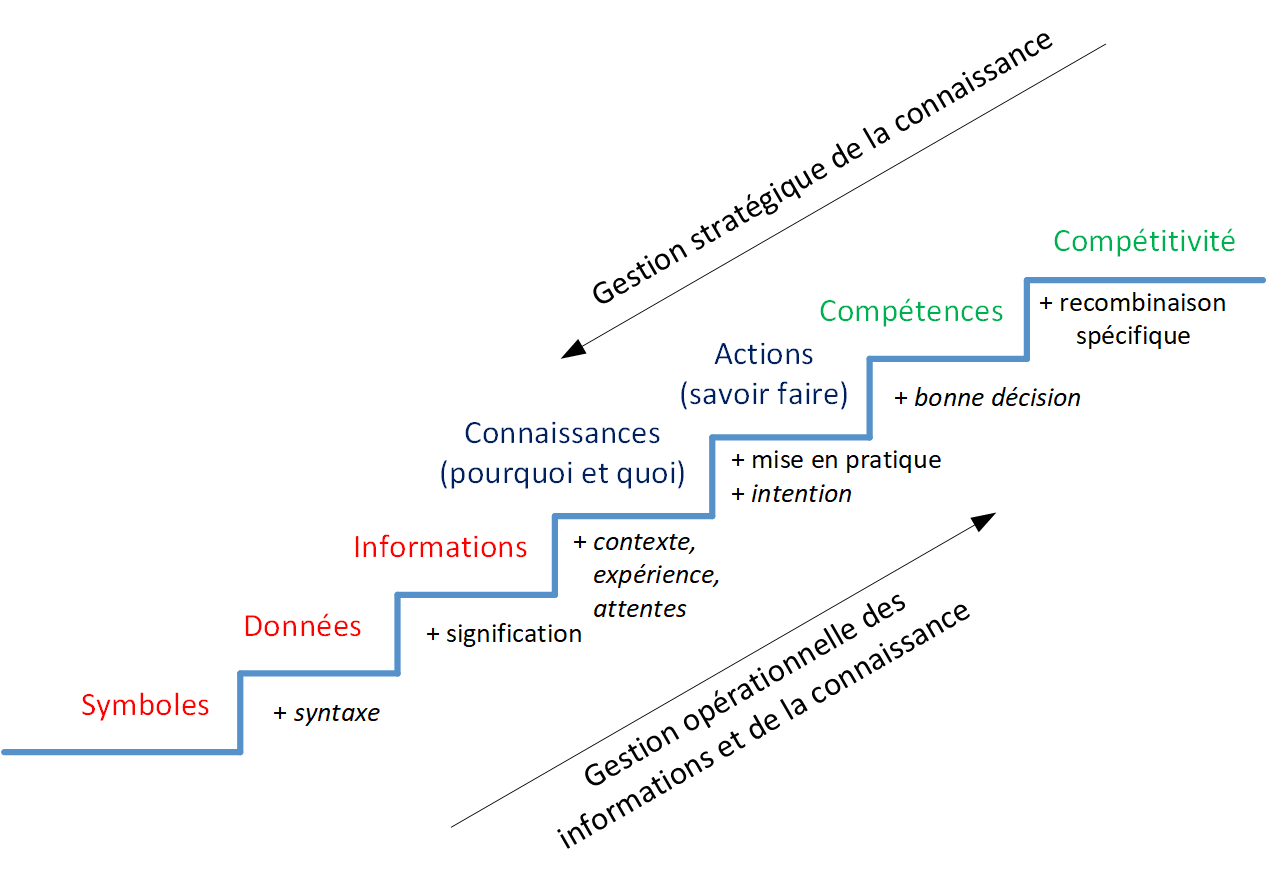
\includegraphics[scale=0.85]{2-Etat-de-l'Art/images/KM/KnowledgeLadder.png}
}
\caption{\'Echelle des connaissances traduite de~\cite{north2018knowledge}}
\label{figure:2-S1-KnowledgeLadder}
\end{figure}


\subsubsection{Connaissances tacites et explicites}
\label{subsubsection:Contexte:KIP-RevueLitterature:KM:ConnaissancesTacitesExplicites}

Les \textit{connaissances explicites} sont formalisées, structurées, systématiques, codifiées et peuvent donc aisément être manipulées, conservées, et partagées~\cite{north2018knowledge}\cite{syed2018palgrave}\cite{nonaka2007knowledge}\cite{nonaka2000seci}.
Les écrits et schémas sont les exemples typiques de connaissances explicites permettant de les transférer facilement d'un individu à l'autre.
Les aspects formel et structuré sont particulièrement visibles dans les formules mathématiques et les spécifications techniques.
Un exemple concret abordé dans~\cite{nonaka2007knowledge} concerne la conception d'une machine à pain dont le pétrissage est insatisfaisant.
Afin d'améliorer le pétrissage, un boulanger expert est observé afin de recopier sa technique et permettre à la machine de générer des pâtes d'une qualité similaire aux siennes.
Les connaissances explicites pouvant être extraites concernent les spécifications de la pâte en entrée puis en sortie, c'est-à-dire ses qualités mesurables (dureté, humidité, ...).

\bigskip

Les \textit{connaissances tacites} concernent au contraire toute l'expertise acquise par un individu au travers de ses sens et de ses facultés.
Les gestes d'un artisan, ou l'intuition issue d'expériences personnelle sont des exemples typiques de connaissances tacites~\cite{north2018knowledge}\cite{syed2018palgrave}\cite{nonaka2007knowledge}.
Ces connaissances sont particulièrement difficiles à transmettre car elles dépendent complètement de l'individu et ne peuvent pas être formalisées ou exprimées aussi facilement que les connaissances explicites.
La transmission de certaines connaissances tacites peut se faire au travers de l'apprentissage : un \textit{maître} exécute des gestes, et son \textit{apprenti} les répète jusqu'à pouvoir les maîtriser, ou au moins les répéter seul pour s'améliorer de lui-même (voire pour développer sa propre technique).
Dans l'exemple de la machine à pain et du boulanger observé~\cite{nonaka2007knowledge}, les connaissances tacites concernent la technique du pétrissage manuel.
Le boulanger peut expliquer succinctement quelques étapes, mais l'expertise précise transformant la pâte implique de répéter le geste et ressentir ses effets.
Une ingénieure a donc pratiqué la technique de pétrissage avec le boulanger pour comprendre le geste et ses effets, afin de pouvoir en déduire les parties manquantes dans la machine à pain conçue.

Appliqué à l'enseignement, on peut retrouver les connaissances qu'un enseignant souhaite transmettre à ses étudiants en s'appuyant sur des connaissances explicites (le syllabus, les notions ciblées, et le support de cours associé) et les connaissances tacites de l'enseignant (expérience personnelle en tant qu'ancien étudiant, cours déjà enseignés dans le passé, par exemple).
Les connaissances tacites constituent précisément dans ce cas une valeur ajoutée à l'enseignant : choix dans l'ordre des notions présentées, accent mis sur certaines d'entre elles selon le profil des étudiants, et explications préférées par chaque groupe d'étudiants.

\bigskip

\subsubsection{Cycle SECI}
\label{subsubsection:Contexte:KIP-RevueLitterature:KM:SECI}

Ces deux types de connaissances participent à un cycle dénommé \textit{SECI}~\cite{nonaka2007knowledge} (Socialisation, Extériorisation, Combinaison, Intériorisation) illustré par la figure~\ref{figure:2-S1-ModeleSECI}.
Ce cycle s'appuie sur les quatre façons de créer et transformer des connaissances : de tacite à tacite (socialisation), de tacite à explicite (extériorisation), d'explicite à explicite (combinaison), d'explicite à tacite (intériorisation).
Chacune de ces façons correspond à des situations particulières qui se répètent :

\bigskip

\begin{itemize}
\item Socialisation (de tacite à tacite) : Deux individus partagent des connaissances tacites par la socialisation.
Il s'agit précisément de la relation où un apprenti observe, imite, et pratique ce que le maître fait, c'est-à-dire un transfert d'expérience d'une personne à l'autre.
La socialisation repose sur l'accumulation et le transfert de connaissances tacites d'un individu à l'autre.\\

\item Extériorisation (de tacite à explicite) : L'extériorisation de connaissances tacites permet de les expliciter, c'est-à-dire les formaliser et en tirer une expérience utile à l'avenir.
Modéliser un processus est une forme d'extériorisation, tout comme décrire le déroulement d'un projet pour pouvoir apprendre des points positifs et éviter certaines erreurs.
L'extériorisation repose sur l'articulation de connaissances tacites des membres d'un groupe pour pouvoir les traduire en concepts explicites.\\

\item Combinaison (d'explicite à explicite) : Plusieurs sources de connaissances explicites, telles que des documents ou des informations, peuvent être combinées pour générer de nouvelles connaissances explicites.
Lire plusieurs rapports ou articles pour en déduire une décision stratégique ou une nouvelle piste de recherche et présenter ces résultats aux collaborateurs sont des exemples.
La combinaison repose sur la recherche et l'intégration de connaissances explicites existantes, pour pouvoir en générer de nouvelles et les diffuser aux groupes d'une organisation.\\

\item Intériorisation (d'explicite à tacite) : Une fois de nouvelles connaissances explicites reçues, un individu les intériorise en les utilisant dans ses activités.
Un ingénieur en lisant une documentation formalisée découvrira des nouveautés qu'il pourra mettre en application par la suite et se les approprier, créant des connaissances tacites.
L'intériorisation concerne un individu qui apprend de nouvelles connaissances explicites au sein d'un groupe ou d'une organisation et se les approprie par la pratique, créant ainsi des connaissances tacites.
\end{itemize}


\begin{figure}[ht]
\centering
\centerline{  % FORCE FIGURE OUTSIDE THE MARGIN !!! BUT STILL CENTERING !!!
% scale = 0.7
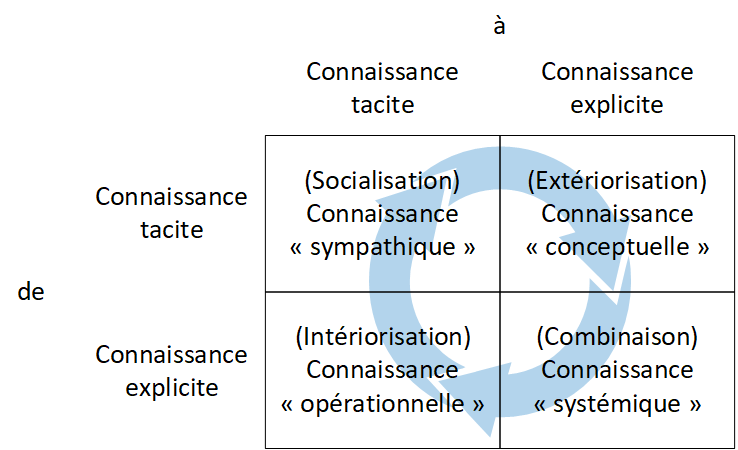
\includegraphics[scale=1]{2-Etat-de-l'Art/images/KM/ModeleSECI.png}
}
\caption{Modèle SECI de~\cite{nonaka2007knowledge} (traduction française de~\cite{tebourbi2000apprentissage})}
\label{figure:2-S1-ModeleSECI}
\end{figure}

\bigskip

Dans l'enseignement supérieur et la recherche, ce cycle se retrouve à différentes échelles.
Lors d'une conférence, des chercheurs vont présenter leurs contributions (extériorisation) et discuter les uns avec les autres (socialisation), ce qui peut engendrer la création d'une nouvelle communauté de recherche partageant des objectifs communs (combinaison) et dont chaque membre développera de nouveaux travaux selon sa propre expérience et son contexte personnel (intériorisation).

Pour un cours, les supports de cours représentent les connaissances explicites, et les échanges entre enseignant et étudiants représentent les connaissances tacites.
Un enseignant s'informera tout d'abord sur le sujet à enseigner en recherchant plusieurs sources (combinaison).
Ensuite, l'enseignant lira les sources pour s'imprégner du sujet et sélectionner les parties à présenter aux étudiants selon ses exigences (intériorisation).
Enfin, l'enseignant délivrera son cours lors de séances en travaux dirigés ou éventuellement en cours magistraux en s'appuyant sur un support de cours formel (extériorisation).
Les travaux dirigés étant particulièrement adaptés aux questions individuelles, et donc à l'apprentissage pas à pas (socialisation), cette étape est répétée en parallèle du cours magistral.
À la fin de chaque séance, l'enseignant vérifie l'avancement par rapport aux objectifs fixés (intériorisation) pour éventuellement modifier son support de cours en conséquences par rapport à ses sources (combinaison).

Inversement, du côté des étudiants, ceux-ci reçoivent un support de cours qu'ils doivent lire (intériorisation) et mettre en pratique lors des travaux dirigés (socialisation).
Les notes de cours prises (extériorisation) sont relues (combinaison) pour pouvoir se préparer aux séances suivantes.
Les notes de cours, devoirs, examens, et présentations sont des exemples de mise en forme explicite de connaissances tacites acquises.

\bigskip

L'exemple de l'enseignement montre que l'ordre des étapes n'est pas toujours rigoureusement le même, mais respecte constamment la transition entre chaque type de connaissances : les étudiants peuvent éventuellement travailler en groupe après une séance (socialisation) avant un examen (extériorisation).
Les connaissances tacites sont échangées entre camarades avant d'être explicitées dans un examen ou dans une présentation dont les membres recombineront les informations au fur et à mesure.

\bigskip

Ces activités centrées sur les connaissances, qu'elles soient tacites ou explicites, sont au c\oe{}ur de processus actuellement difficiles à gérer pour de nombreuses raisons.
Les individus et leurs connaissances tacites sont un exemple de difficulté : il est impossible de savoir à l'avance quelles connaissances tacites un individus possèdera en lui, ni les décisions qu'il prendra.
Un domaine de recherche s'intéresse en particulier aux défis posés par les connaissances dans les processus au sein des organisations, c'est-à-dire aux \textit{processus à forte intensité de connaissances}, que nous présentons dans les sous-sections suivantes.


\bigskip

%%%%%%%%%%%%%%%%%%%%%%%%%%%%%%%%%%%%%%%%%%%%
%\clearpage % Clean for pictures and tables %
%\newpage   % Clean for pictures and tables %
%%%%%%%%%%%%%%%%%%%%%%%%%%%%%%%%%%%%%%%%%%%%

\subsection{Les processus à forte intensité de connaissances}
\label{subsection:Contexte:KIP-RevueLitterature:KIP}

Observer des phénomènes se produire, c'est observer des processus s'exécuter.
Les processus tirent leurs origines linguistiques du latin \textit{processus} ou \textit{processioat} qui signifient \textit{action exécutée} ou \textit{quelque chose de fait}, et la \textit{façon dont elle a été faite}~\cite{von2014complete}.
Depuis Adam Smith et Frederick Taylor, le point de vue général adopté sur les processus métier est centré sur les activités, en particulier sur des tâches et leur ordonnancement~\cite{boissier2019challenges}.
Au sein des organisations actuelles, de nombreux processus métier sont modélisés et pris en charge par la \textit{gestion de processus métier}, ou \textit{business process management}~\cite{weske2007business} (BPM) en anglais.
Certains processus centrés sur les connaissances sont cependant encore difficiles à gérer au sein des systèmes d'informations~\cite{boissier2019challenges}, il s'agit des \textit{processus à forte intensité de connaissances}, ou \textit{knowledge intensive processes} (KIP) en anglais.
Des synonymes peuvent être retrouvés dans la littérature tels que \textit{knowledge intensive business processes}~\cite{icsik2013practices}\cite{manfreda2015knowledge} ou \textit{artful processes}~\cite{hill2006beyond}, mais certains autre termes comme \textit{case}~\cite{davenport1994case}\cite{van2005case} ont une signification un peu plus particulière que nous présentons par la suite.

\bigskip

Comme présenté dans la sous-section précédente, les connaissances tacites et explicites impliquent certaines spécificités lors de leur intégration dans les systèmes d'informations.
Les connaissances explicites sont par définition formalisées et visent à être transmises, celles-ci sont donc plus facilement intégrées aux méthodes classiques de gestion des processus.
En effet, les activités de modélisation de processus, visant à formaliser un processus en le représentant sous forme de schéma, sont déjà intégrées dans le cycle de vie du BPM et sont un exemple d'extériorisation.
Un autre exemple illustrant cette fois la combinaison concerne la rédaction des rapports annuels : les informations agrégées sont directement issues du système d'informations, parfois même de façon automatique.
À l'inverse, les connaissances tacites étant par définition informelles et uniques à chaque individu, celles-ci sont beaucoup moins aisées à gérer.
La socialisation peut éventuellement être facilitée par l'organisation d'évènements ou d'ateliers, mais l'intériorisation est au contraire une étape totalement individuelle et ne peut donc pas simplement être provoquée par une volonté extérieure.

L'étude des processus à forte intensité de connaissances s'intéresse particulièrement, mais pas exclusivement, aux connaissances tacites afin de mieux les prendre en charge et exploiter leur potentiel.
L'importance des connaissances dans ces processus leur confère plusieurs caractéristiques et exigences telles que la flexibilité dans l'ordre des activités, des évènements inattendus impliquant des tâches imprévisibles (donc absentes des modèles de processus conçus à priori), de la créativité, et bien d'autres.

\bigskip

\subsubsection{Caractéristiques des KIP}
\label{subsubsection:Contexte:KIP-RevueLitterature:KIP:CaracteristiquesKIP}

Plusieurs études ont cherché à comprendre plus en profondeur les KIP et leurs caractéristiques afin de pouvoir, si possible, les intégrer aux outils et méthodes BPM déjà en place.
Les travaux présentés dans~\cite{icsik2013practices} ont cherché dans la littérature les différences entre les KIP et les processus métier plus traditionnels.
La plupart des caractéristiques n'opposent pas directement les deux types de processus, mais les KIP en accentuent certaines.
Typiquement, \og \textit{les degrés exigés de complexité, répétabilité, et créativité ne sont pas les mêmes, mais ils ne sont pas moins éligibles à l'automatisation ou l'organisation structurée} \fg~\cite{icsik2013practices} (\og \textit{different levels of complexity, repeatability and creativity required for these processes, but are not necessarily less eligible for automation or structured} \fg~\cite{icsik2013practices}).
Cependant, l'article conclut tout de même que les KIP sont \og \textit{plus complexes, moins répétables, et exigent beaucoup de créativité} \fg~\cite{icsik2013practices}.

\bigskip

Les travaux dans~\cite{di2015knowledge} insistent tout d'abord sur les liens entre le BPM et le domaine du KM qu'il faut développer.
En effet, la connaissance est un élément clé jusque là peu exploité dans le BPM, alors qu'elle contient d'après~\cite{davenport2005thinking} \og \textit{l'expérience, le contexte, l'interprétation et la réflexion, et implique plus de coopération humaine que d'informations} \fg~\cite{di2015knowledge} (\og \textit{experience, context, interpretation and reflection and involves more human participation than information} \fg~\cite{di2015knowledge}).
Cette vision met l'accent sur les connaissances tacites, étant donné que les connaissances explicites s'appuient sur des informations et des données déjà connues des systèmes d'informations, et donc des méthodes BPM mises en place.
Plusieurs autres définitions sont également étudiées, mais une en particulier~\cite{vaculin2011declarative} insiste sur le rôle des \textit{travailleurs du savoir} (\textit{knowledge workers} en anglais) qui effectuent des tâches impliquant des prises de décisions à forte intensité de connaissances, c'est-à-dire en rassemblant de nombreuses informations pour en générer de nouvelles, voire pour produire des artefacts (par exemple des plans, des recommandations, ou encore des exigences liés aux décisions prises).
Une définition des \textit{artful processes} proposée dans~\cite{hill2006beyond} insiste également sur l'importance des individus exécutant le processus et surtout leurs connaissances tacites (\og \textit{compétences, expérience, jugement} \fg~\cite{hill2006beyond}) : le processus, voire les tâches, sont définissables d'un point de vue haut niveau, mais il est impossible de fixer à l'avance les détails.
\cite{di2015knowledge} souligne également le fait qu'un \textit{artful process} est en fait défini par les personnes (et leurs connaissances) qui l'exécutent : il n'est pas possible de définir un processus à proprement parler, mais il faut plutôt parler de l'instance en elle-même.

\bigskip

Toujours dans~\cite{di2015knowledge}, huit caractéristiques des KIPs ont été retenues et sont présentées afin d'en déduire vingt cinq exigences.
Les KIPs y sont considérés comme :
\begin{itemize}
\item Dirigés par les connaissances (\og \textit{knowledge-driven} \fg) : les données et connaissances disponibles servent à prendre les décisions et donc à diriger le processus.
\item Orientés collaboratif (\og \textit{collaboration-oriented} \fg) : le contexte d'exécution du processus est collaboratif et multi-utilisateurs, et les connaissances et artefacts générés (autant par les humains que par l'instance de processus) sont partagés.
\item Imprédictibles (\og \textit{unpredictable} \fg) : chaque instance dispose de son propre contexte et d'éléments imprévisibles qui font varier les connaissances exploitées, le flot d'exécution, et l'ordre des tâches d'une instance à l'autre.
\item Émergents (\og \textit{emergent} \fg) : l'exécution du processus fait émerger au fur et à mesure des informations qui permettent de choisir les actions et décisions à prendre.
\item Orientés buts (\og \textit{goal-oriented} \fg) : des buts intermédiaires servent à avancer dans l'exécution du processus.
\item Dirigés par les évènements (\og \textit{event-driven} \fg) : les décisions prises par les travailleurs du savoir pour avancer dans l'exécution du processus dépendent des évènements rencontrés.
\item Dirigés par les contraintes et les règles (\og \textit{constraint- and rule-driven} \fg) : les actions et décisions prises par les utilisateurs sont guidées par des règles ou contraintes à respecter.
\item Non-répétables (\og \textit{non-repeatable} \fg) : les situations variant à chaque instance de processus, il est quasiment impossible de parfaitement répéter une précédente exécution.
\end{itemize}

\bigskip

Ces caractéristiques ne sont pas exhaustives, étant donné que le domaine est toujours actif et que les tâches non-liées à un système ou environnement d'exécution BPM n'ont pas été complètement dénombrées, mais elles sont particulièrement pertinentes.
Une réunion, par exemple, implique par définition de la collaboration entre toutes et tous les participants, chaque point de l'ordre du jour doit être abordé (buts intermédiaires), elle est dirigée par les connaissances partagées au fur et à mesure des discussions et des points de vues de chacun, certains sujets seront peut être plus développés que d'autres (émergence et imprédictibilité), voire, la réunion peut être interrompue par un évènement inattendu.
Dans tous les cas, il sera impossible de répéter scrupuleusement la réunion dans sa séquence et son contenu.

Il faut tout de même retenir qu'un KIP ne répond pas nécessairement à l'ensemble de ces caractéristiques, mais au moins à certaines d'entre elles.
Le développement d'un logiciel peut tout à fait se réaliser seul (et sans utiliser de forum d'entre-aide) : il suffit d'avoir des connaissances en développement logiciel, et de respecter les limitations imposées par la machine et système d'exploitation ciblés.
Cependant, ce logiciel sera peu réutilisable en l'absence de documentation explicitant le contexte précis d'utilisation.
De plus, l'absence de prise en compte des retours utilisateurs (d'ailleurs souvent issus de \textit{l'expérience utilisateur}) limitera les évolutions.
Les différentes méthodes agiles de développement d'applications~\cite{fowler2001agile} visent justement à essayer d'intégrer au mieux toutes ces caractéristiques : fixer des buts intermédiaires régulièrement, prévoir de la collaboration entre développeurs et utilisateurs, s'adapter au changement et limiter l'impact des évènements imprévus, ... tout en essayant de produire les applications les plus réutilisables possibles mais en s'adaptant au contexte de chaque cas.


\bigskip


\subsubsection{Difficultés pour gérer les KIP}
\label{subsubsection:Contexte:KIP-RevueLitterature:KIP:DifficulteGestionKIP}

Les participants et leurs connaissances sont donc au c\oe{}ur de ces processus dont les caractéristiques précédemment relevées sont difficilement intégrables telles quelles dans l'environnement BPM classique~\cite{riss2005challenges}\cite{moura2013collaboration}.
Nous avons identifié six défis concernant les KIPs et les avons décrits dans une publication~\cite{boissier2019challenges}.

\begin{enumerate}
\item \og \textit{Comment gérer de façon efficiente et efficace les connaissances et informations manipulées (c'est-à-dire créées, utilisées, mises à jours) par les KIPs ?} \fg
L'absence de gestion des connaissances et des informations impacte négativement les KIPs.
Les travaux de~\cite{hislop2018knowledge} exposent justement les difficultés auxquelles font face dans la pratique les organisations dans la gestion des grandes quantités d'informations.
Bien que le domaine des \textit{Mégadonnées} (\textit{Big Data} en anglais) et ses 3V visent les problèmes liés aux \textit{Volume, Vélocité et Variété}, il s'agit de manipuler des \textit{données} et non pas des \textit{informations} ni des \textit{connaissances}~\cite{delort2018big}.\\

\item \og \textit{Comment supporter l'aspect collaboratif et les prises de décisions spécifiques au contexte dans les KIPs ?} \fg
Les organisations ont plutôt tendance à standardiser et contrôler les processus~\cite{riss2005challenges}, or, limiter la collaboration et la créativité limite les capacités des utilisateurs~\cite{gromoff2017business} et contrevient aux caractéristiques mêmes des KIPs.
Bien que des solutions tentent d'améliorer les communications informelles~\cite{di2011mailofmine}, l'aspect collaboratif entre les participants aux KIPs reste un défi à relever~\cite{moura2013collaboration}.\\

\item \og \textit{Comment intégrer les informations de contexte lors de la conception d'un KIP ?} \fg
Le contexte d'exécution d'un KIP sous-entend la situation ou l'environnement d'exécution (l'état de l'organisation, des équipes impliquées, ou de la société en général) ainsi que les connaissances tacites des participants au KIP.
Prévoir lors de la conception d'un processus dans quelle situation sera l'organisation et quelles seront les connaissances tacites des utilisateurs est quasiment impossible : chaque instance de KIP étant unique, des activités ou évènements inattendus peuvent se produire et apporter de nouvelles expériences aux utilisateurs qui ne répèteront pas nécessairement le même cheminement y compris si un cas similaire se reproduit.
Le paradigme déclaratif~\cite{tran2015embracing} permet à minima de proposer des règles et un cadre à respecter, mais aussi dans lequel évoluer.
Le contexte n'est donc pas complètement prévisible ni intégré, mais certaines conditions d'exécutions peuvent indiquer quelles activités faire ou préférer.\\

\item \og \textit{Comment supporter la conformité dans les KIPs ?} \fg
Par définition, le paradigme impératif du BPM simplifie la mise en place de règles de conformité.
Le domaine de la \textit{gestion de règles métier}~\cite{ross2003manifesto}, ou \textit{Business Rules Management} (BRM) en anglais, apporte une réponse particulièrement adaptée en séparant les règles des processus~\cite{zur2007business}.
Comme indiqué dans le défi précédent : le paradigme déclaratif offre des pistes pour cadrer les KIPs, mais assurer une conformité stricte de façon automatisée est encore difficile.
Le déroulement des activités dépendant surtout des décisions prises par les participants~\cite{kushnareva2015modelingStatecharts}, ces derniers ont donc majoritairement un contrôle sur le processus et donc la responsabilité concernant le respect de la réglementation.
Une autre contrainte réside aussi dans le fait que la règlementation est exprimée dans le langage naturel, voire avec des spécificités du droit, et qu'il est parfois long et difficile de les transformer en règles métier accessibles aux utilisateurs des KIPs~\cite{zur2007business}.
Quelques solutions sont néanmoins étudiées pour simplifier cette transformation~\cite{zasada2018box}.\\

\item \og \textit{Comment supporter la flexibilité dans les KIPs ?} \fg
L'imprédictibilité et la créativité, mais aussi l'émergence et les évènements se produisant au fil du temps, impliquent que les utilisateurs de KIPs ont besoin d'une grande liberté d'action.
Comme nous l'avons vu, il s'agit cependant aussi de restreindre cette liberté selon les réglementations du domaine, voire, les contraintes liées au contexte particulier du cas étudié.
La flexibilité nécessaire pour entretenir une certaine liberté d'action, tout en respectant les contraintes, est grandement étudiée dans la littérature~\cite{riss2005challenges}\cite{herrmann2011adaptive}\cite{huber2015adaptive}\cite{tran2015embracing}\cite{de2016modeling}\cite{gromoff2017business}\cite{zensen2018comparison}, car il s'agit d'un problème encore ouvert.\\

\item \og \textit{Comment explorer et réutiliser des fragments de processus dans les KIPs ?} \fg
Le domaine du \textit{raisonnement à base de cas}~\cite{slade1991case}, ou \textit{Case-Based Reasoning} (CBR) en anglais, vise à ré-\og \textit{utiliser les expériences passées pour comprendre et résoudre de nouveaux problèmes} \fg~\cite{kolodner1992introduction} (\og \textit{using old experiences to understand and solve new problems} \fg~\cite{kolodner1992introduction}).
Cette idée a été étudiée dans quelques travaux~\cite{di2015knowledge}\cite{cognini2016case} en proposant aux utilisateurs des KIPs des \textit{motifs} (ou \textit{patterns} en anglais) issus d'instances précédemment exécutées.
La validation des motifs par des experts du domaine peut permettre leur réutilisation en accord avec les règles en place.
Ces motifs, selon leur nature, peuvent également embarquer une partie du contexte des exécutions précédentes sans intervention manuelle, et donc répondre à plusieurs défis précédemment énoncés.\\

\end{enumerate}

\bigskip

Comme nous venons de le voir, les KIPs font encore face à de nombreux défis partiellement interdépendants.
Plusieurs domaines de recherche connexes contribuent à affiner les réponses possibles, mais ne permettent pas en l'état d'intégrer les KIPs aux systèmes d'informations s'appuyant uniquement sur le BPM.
La littérature propose plusieurs points de vues sur les KIPs permettant de mieux se concentrer sur certains défis.



\bigskip

%%%%%%%%%%%%%%%%%%%%%%%%%%%%%%%%%%%%%%%%%%%%
%\clearpage % Clean for pictures and tables %
%\newpage   % Clean for pictures and tables %
%%%%%%%%%%%%%%%%%%%%%%%%%%%%%%%%%%%%%%%%%%%%

\subsection{Le défi de la réutilisation des fragments de processus et des connaissances}
\label{subsection:Contexte:KIP-RevueLitterature:Reutilisation}

Le raisonnement à base de cas~\cite{slade1991case}\cite{kolodner1992introduction} s'appuie énormément sur la réutilisation des cas passés afin d'en résoudre de nouveaux.
Ce point de vue des cas est issu de la \textit{gestion de cas}~\cite{davenport1994case}\cite{van2005case}\cite{swenson2013white}, ou \textit{case management} en anglais, qui s'appuie sur des pratiques où l'ensemble des informations nécessaires pour réaliser des activités sont rassemblées dans ce qui s'appelle un \textit{cas}~\cite{swenson2013white}.
L'expérience acquise lors d'une activité se répercute dans les connaissances tacites des individus impliqués, et éventuellement sous forme explicite si des traces ou des artefacts ont été générés.
Il s'agit de l'intériorisation dans le cycle SECI présenté précédemment : chaque individu a pratiqué une activité en s'appuyant sur des connaissances explicites qui sont devenues progressivement tacites.
Ces connaissances tacites sont cependant uniques à la situation dans laquelle s'est réalisée l'activité.
Réutiliser ces connaissances implique que l'individu se retrouve dans une situation similaire, c'est-à-dire que le contexte soit suffisamment proche pour qu'il puisse adapter ses actions.

La réutilisation des connaissances est étudiée dans la littérature, mais beaucoup moins que plusieurs autres étapes intervenant avant la réutilisation en elle-même~\cite{schacht2016methodology} que nous décrivons par la suite.
Du point de vue des processus à forte intensité de connaissances, les fragments de processus permettent de s'appuyer sur l'expérience des individus dans leurs activités pour extraire un sous-ensemble de tâches et activités afin de les réutiliser lors de la conception et de l'exécution.


\bigskip


\subsubsection{Le défi de la réutilisation dans le cas de la gestion des connaissances connaissances}
\label{subsubsection:Contexte:KIP-RevueLitterature:ReutilisationKIP:KM}


Les travaux présentés dans~\cite{markus2001toward} étudient la réutilisation de connaissances sous sa forme de processus avec des rôles et des dépôts de connaissances, pour en déduire quatre types de situations de réutilisation possibles.
Le processus général de gestion des connaissances se divise en quatre étapes :

\begin{enumerate}
\item Capturer ou documenter les connaissances (\og \textit{capturing or documenting knowledge} \fg) : documentation de(s) l'activité(s) par des moyens automatiques ou induits par l'activité(s) elle(s)-même(s) (archivage automatique de messages échangés, par exemple), ou par des structures prévues à la conception (champs obligatoires à remplir, par exemple).\\

\item Empaqueter les connaissances à réutiliser (\og \textit{packaging knowledge for reuse} \fg) : les documents générés sont nettoyés puis mis en forme pour pouvoir être indexés dans un dépôt.
Les informations concernant le contexte sont ajoutées, le contenu des documents est filtré et nettoyé, et des modèles de classification sont développés.\\

\item Distribuer ou disséminer les connaissances (\og \textit{distributing or disseminating knowledge} \fg) : partage des connaissances de façon passive (dépôt alimenté régulièrement par les nouvelles expériences, ou envoi régulier d'une note d'informations, par exemple) ou active (organisation de réunions détaillant un retour d'expérience particulier, par exemple), et activités de facilitation (aide à l'utilisation ou à l'identification de besoins en réutilisation de connaissances, ou mise en place de bonnes pratiques, par exemple).\\

\item Réutiliser les connaissances (\og \textit{reusing knowledge} \fg) : Cette dernière étape se décompose elle-même en quatre activités.
Tout d'abord, \textit{définir la question} (\og \textit{defining the search question} \fg) afin de mobiliser les connaissances et experts les plus aptes à y répondre.
Puis, \textit{chercher et localiser les experts ou les expertises} (\og \textit{the search for, and location of, experts or expertise} \fg), pour pouvoir ensuite \textit{sélectionner l'expert ou le conseil approprié d'un expert} (\og \textit{selection of an appropriate expert or of expert advice} \fg).
Enfin, \textit{appliquer les connaissances} (\og \textit{applying the knowledge} \fg) à la situation actuelle, c'est-à-dire en recontextualisant les connaissances récupérées du dépôt.
Cette dernière étape s'appuie sur deux notions spécialisées sur les connaissances : le \textit{rappel} (\og \textit{recall} \fg) qui permet de savoir si une information a été indexées et la retrouver, et la \textit{reconnaissance} (\og \textit{recognition} \fg) qui permet de savoir si une information répond aux besoins de l'utilisateur et s'applique aux connaissances visées.
Mais aussi sur deux notions spécialisées sur l'expertise humaine : l'\textit{identification} (\og \textit{identification} \fg) d'experts sur un domaine en particulier, et la \textit{sélection} (\og \textit{selection} \fg) de l'expert le plus approprié pour la question.
\end{enumerate}


\bigskip

Trois rôles sont également mobilisés lors de l'exécution de ce processus de réutilisation~\cite{markus2001toward}.
Ces rôles peuvent être tenus par des individus distincts, ou par le même :

\begin{itemize}
\item Producteur de connaissances (\og \textit{knowledge producer} \fg) : la personne qui documente les connaissances en enregistrant les connaissances explicites, ou en transformant les connaissances tacites en connaissances explicites (extériorisation).

\item Intermédiaire de connaissances (\og \textit{knowledge intermediary} \fg) : la personne qui adapte les connaissances pour les réutiliser grâce à l'élucidation, le nettoyage, l'indexation, et l'empaquetage.
Cette personne est également chargée de distribuer les connaissances au sein de l'organisation.

\item Consommateur de connaissances (\og \textit{knowledge consumer} \fg) : la personne qui retrouve et adapte le contenu des connaissances passées pour les appliquer à son cas.
\end{itemize}

\bigskip

De nombreux types de dépôts existent dont les caractéristiques les distinguent les uns des autres~\cite{markus2001toward}.
La plus simple des distinctions s'appuie sur la nature des objets entreposés : les \textit{documents} (texte, audio, vidéo) n'étant pas toujours stockés de la même manière que les \textit{données} (structures de données, systèmes de gestion de base de données relationnelles / SGBDR).
Les travaux dans~\cite{davenport1998successful} distinguent les \textit{connaissances externes}, concernant l'environnement extérieur à l'organisation, les \textit{connaissances internes structurées}, tels que les documents et données, et enfin les \textit{informations informelles}, comme les notes de réunions ou les mails.
Une autre distinction présentée dans~\cite{zack1999managing} concerne la nature des connaissances : les \textit{connaissances générales}, tel que l'état des connaissances scientifiques actuelles, et les \textit{connaissances spécifiques}, tels que les informations et le vocabulaire internes à une organisation.

Dans le contexte actuel où les données et informations sont accessibles quasiment n'importe où, ces dépôts peuvent être assimilés à d'autres formes que les \textit{entrepôts de données} (\og \textit{date warehouses} \fg) ou SGBD traditionnels, comme par exemple les nombreux \textit{wikis}~\cite{schacht2016methodology}.

\bigskip

Ce processus, les rôles, et les dépôts représentent un modèle général de gestion des connaissances dans lequel l'étape de réutilisation intervient relativement tard.
La réutilisation de connaissances implique évidemment de créer et stocker des connaissances, avant de les partager ou de les transférer et éventuellement de les adapter.
Quatre types de situations de réutilisation des connaissances ont été identifiés et sont présentés dans une typologie~\cite{markus2001toward} :

\begin{itemize}
\item \textit{Producteurs collaboratifs} (\og \textit{Shared Work Producers} \fg) : les individus travaillant dans des équipes proches les unes des autres produisent, stockent, partagent et retrouvent leurs propres connaissances pour les réutiliser.
Bien qu'ils n'aient que peu de difficultés à réutiliser leurs connaissances, lorsque les équipes en question stockent beaucoup trop de connaissances, il est parfois difficile et long de retrouver précisément celles recherchées.
Le problème se pose également lorsque ces connaissances ne sont pas numérisées (des brouillons, par exemple) ou qu'elles sont mal renseignées lors de leur enregistrement (contexte mal détaillé).\\

\item \textit{Praticiens collaboratifs} (\og \textit{Shared Work Practitioners} \fg) : les individus affectés à une même fonction mais éloignés géographiquement, dans l'organigramme, ou bien même dans des organisations distinctes, partagent néanmoins des connaissances qu'ils réutilisent.
Les principales difficultés concernent la sélection des connaissances les plus adaptées au problème (les consommateurs n'arrivent pas à évaluer quelles connaissances répondent au mieux à leurs besoins), la réputation des contributeurs (certains contributeurs seront préférés à d'autres), enfin le contexte des connaissances (les consommateurs de connaissances peuvent ne pas connaître ni comprendre le contexte d'origine).\\

\item \textit{Novices cherchant une expertise} (\og \textit{Expertise-Seeking Novices} \fg) : les individus étrangers à un domaine ont besoin d'experts pour les aider à réutiliser des connaissances.
De nombreuses difficultés sont rencontrées par les novices, dont la première est le jargon (la question posée ne contient pas le ou les termes spécifiques qui permettraient de comprendre le problème et retrouver immédiatement les connaissances adaptées), suivie du contexte des informations (un novice peut mélanger le contexte et les informations), et enfin les connaissances doivent être présentées de façon accessible aux non-experts (renvoyer des débutants vers un manuel technique complet ne leur permet pas d'identifier précisément la connaissance recherchée).\\

\item \textit{Explorateurs tiers de connaissances} (\og \textit{Secondary Knowledge Miners} \fg) : les individus effectuant de l'exploration de données peuvent également réutiliser des connaissances et en générer de nouvelles.
Ces utilisateurs ne connaissent pas toujours le contexte exact dans lequel les données ont été extraites ni l'objectif initial.
Il est donc conseillé de fournir une formation solide aux utilisateurs effectuant de l'exploration de données afin qu'ils maîtrisent les limites des ensembles qu'ils manipulent.
\end{itemize}

\bigskip

La plupart des réponses pour dépasser ces limites concernent la documentation : documenter pour soi-même afin de pouvoir retrouver, comprendre, et réutiliser ses propres connaissances, documenter pour les pairs du domaine afin de les orienter vers les connaissances les plus adaptées, et enfin documenter pour les novices afin de leur permettre d'adapter les connaissances à leur cas (en retirant l'excès de contexte avant de les leur fournir) et d'éviter l'excès de données pouvant entraîner de mauvaises interprétations.
Concrètement, dans les projets informatiques actuels, on peut retrouver cette documentation dans les commentaires d'un code, dans les notes des outils de gestion de versions, voire dans les wikis.

\bigskip

D'autres travaux~\cite{petter2009developing} décrivent trois méthodes de réutilisation observées dans le cas des projets informatiques d'une société de conseils :

\begin{itemize}
\item Le \textit{verbatim} (\og \textit{verbatim} \fg) : les connaissances sont directement réutilisées sans aucune adaptation (en répétant par exemple rigoureusement les mêmes étapes).
Cette méthode ne fonctionne pas toujours étant donné que les situations varient constamment et qu'il est difficile de retrouver un contexte suffisamment proche pour que les connaissances soient parfaitement réutilisables telles quelles.
Cependant, l'usage du verbatim à des fins heuristiques a fonctionné (par exemple estimer la durée d'exécution d'une tâche à partir d'exécutions passées).\\

\item La \textit{synthèse} (\og \textit{synthesis} \fg) : plusieurs sources de connaissances sont combinées afin de construire une solution adaptée au cas présent (plusieurs expériences similaires passées sont analysées ainsi qu'une liste de bonnes pratiques, afin de résoudre un nouveau problème).
Cette méthode s'appuie à la fois sur des connaissances explicites et les connaissances tacites de l'individu construisant sa solution.
L'intérêt majeur repose sur le fait que des réponses proches existent déjà, et que l'on ne construit pas une réponse à partir de rien.\\

\item La \textit{création} (\og \textit{creation} \fg) : une nouvelle solution est construite à partir de rien en effectuant des sessions de réflexion ou des réunions, c'est-à-dire en s'appuyant sur la sagesse collective.
Cette méthode est surtout utilisée dans les situations difficiles, et lorsque les autres méthodes ne fonctionnent pas.
Les réunions permettent d'exposer les problèmes et exigences à respecter pour en déduire de nouvelles solutions et leurs conséquences grâce à l'expérience de chaque individu (la simple combinaison de solutions passées n'est pas suffisante, et il est nécessaire de reprendre le problème depuis le début).
\end{itemize}

\bigskip

L'étude menée dans~\cite{ajmal2008knowledge} a montré que les solutions déployées servaient principalement à accumuler les connaissances et n'étaient jusque là que peu utilisées en pratique.
De plus, selon~\cite{schacht2016methodology}, les chercheurs et les praticiens s'intéressent plutôt à la collecte, au stockage, et au transfert de connaissances plutôt qu'à la réutilisation.
Plus précisément, l'analyse faite par~\cite{schacht2016methodology} explique que les études réalisées avec une méthodologie orientée \textit{behavior} visent à expliquer et comprendre les phénomènes, mais elles ne donnent aucune recommandation pour les praticiens.
À l'inverse, les solutions construites avec une méthodologie \textit{science du design} sont trop orientées vers les fonctionnalités, et elles ne vérifient donc pas les conséquences sur l'organisation ou les comportements des individus.

\bigskip

Du point de vue de la gestion des connaissances, la réutilisation des connaissances est donc un problème encore ouvert.
Peu de travaux de recherche s'y sont spécifiquement intéressés, et les solutions techniques proposent des fonctionnalités plutôt liées aux activités avant la réutilisation (c'est-à-dire l'acquisition, le stockage, et le transfert).


\bigskip


\subsubsection{Le défi de la réutilisation de fragments de processus dans le cas des processus à forte intensité de connaissances}
\label{subsubsection:Contexte:KIP-RevueLitterature:Reutilisation:KIP}

Dans le domaine des processus à forte intensité de connaissances, la réutilisation de fragments est également un des défis actuellement étudiés~\cite{boissier2019challenges}.
Les travaux de~\cite{eberle2009process}\cite{eberle2010process} donnent une définition des \textit{fragments de processus} en indiquant qu'il s'agit des activités, et des connaissances qui y sont attachées, auxquelles chaque participant au processus est assigné selon son propre contexte local.
La notion \textit{locale} est importante dans le sens où chaque fragment est lié à la fois à une partie d'un processus (un sous-ensemble d'activités), à un individu exécutant les activités impliquées, et aux connaissances mobilisées à l'exécution de ces activités.
Lors de l'inscription d'un étudiant à l'université par exemple, l'étudiant dispose de son propre fragment sur l'expérience utilisateur, les personnels administratifs des inscriptions vérifient et répondent, et enfin, les personnels administratifs des unités des formation et de recherche attribuent un groupe à chaque étudiant selon les filières.
La figure~\ref{figure:2-S1-KIP-Exemple-Fragments} expose les trois fragments de ce processus d'inscription.
Chaque fragment mobilise donc des connaissances spécifiques : générer les pièces de son propre dossier, vérifier la validité des pièces et cas particuliers puis envoyer les documents réponses, construire les groupes d'étudiants selon les exigences de la formation et des salles disponibles.
L'objectif des travaux présentés dans~\cite{eberle2010process} visent à proposer à un expert de réutiliser des fragments de processus structurés lors de la conception des processus, mais également lors de leur exécution.


%\begin{figure*} % Figure flottante
\begin{figure}[ht]
\centering
\centerline{
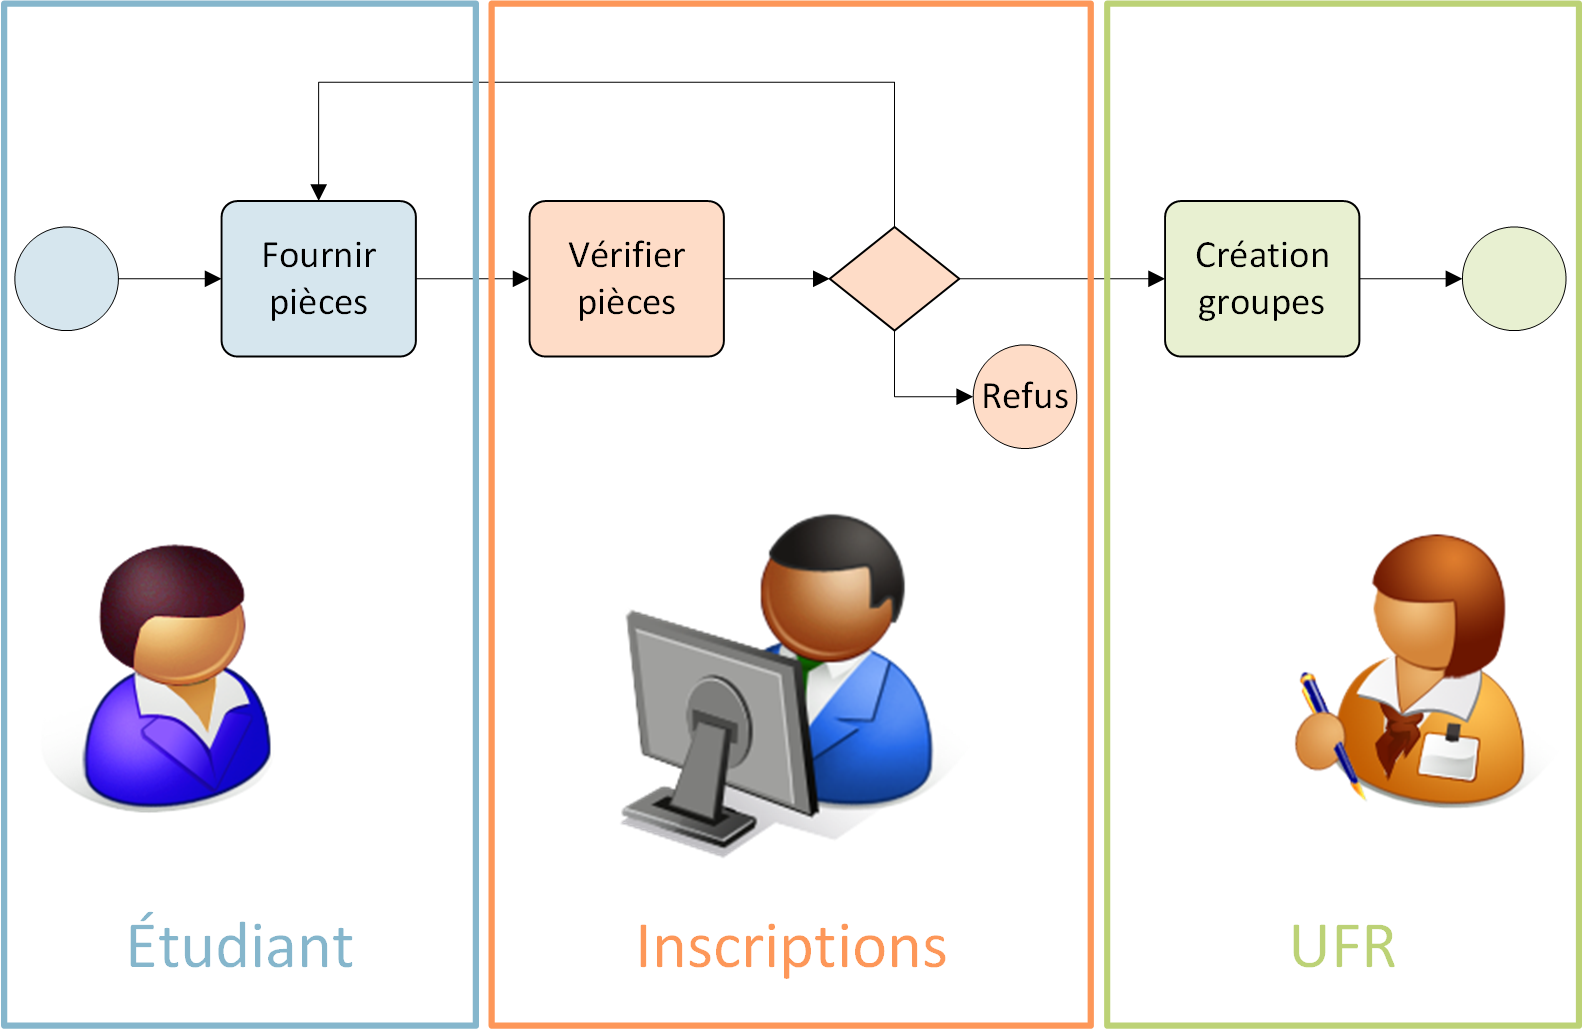
\includegraphics[scale=0.65]{2-Etat-de-l'Art/images/KIP/Fragments/FragmentsProcessus.png}
}
\caption{Exemple d'un processus d'inscription d'étudiant et de ses trois fragments}
\label{figure:2-S1-KIP-Exemple-Fragments}
\end{figure}
%\end{figure*} % Figure flottante
% To use it : fig~\ref{label}

\bigskip

Une amélioration de l'usage de ces fragments de processus a été proposée dans les travaux présentés dans~\cite{cognini2016case} en s'inspirant des techniques de CBR~\cite{slade1991case}\cite{kolodner1992introduction} afin de gérer des cas, et non plus des processus structurés.
Le CBR s'appuie sur un schéma en plusieurs étapes rappelant énormément celui appliqué en gestion des connaissances :
\begin{enumerate}
\item une personne décrit tout d'abord au système le problème auquel elle est confrontée,
\item le système recherche les cas similaires dans sa base de cas,
\item le système sélectionne le cas le plus proche afin de le réutiliser,
\item le système adapte le cas retenu au contexte actuel,
\item si la personne valide le cas adapté, celui-ci est retenu et est conservé à son tour pour un possible ré-usage futur.
\end{enumerate}

\bigskip

Les systèmes de gestion des cas s'étant développés dans un environnement statique et contrôlé, ils ne sont pas adaptés aux situations exigeant de la flexibilité~\cite{motahari2013adaptive}.
Ainsi, l'\textit{Adaptive Case Management} (ACM)~\cite{swenson2010mastering} s'est développé pour pouvoir s'affranchir des contraintes et permettre aux participants d'adapter le système aux cas rencontrés et aux évènements émergents.
La figure~\ref{figure:2-S1-KIP-Exemple-ACM} illustre la différence entre le point de vue classique impératif où un processus est modélisé de façon détaillée, et les traces d'exécutions contiennent la progression des instances, tandis que le point de vue cas s'intéresse aux intervenants qui les traitent en consultant, ajoutant, modifiant, ou supprimant des données au fur et à mesure.

\begin{figure}[ht]
\centering
\centerline{
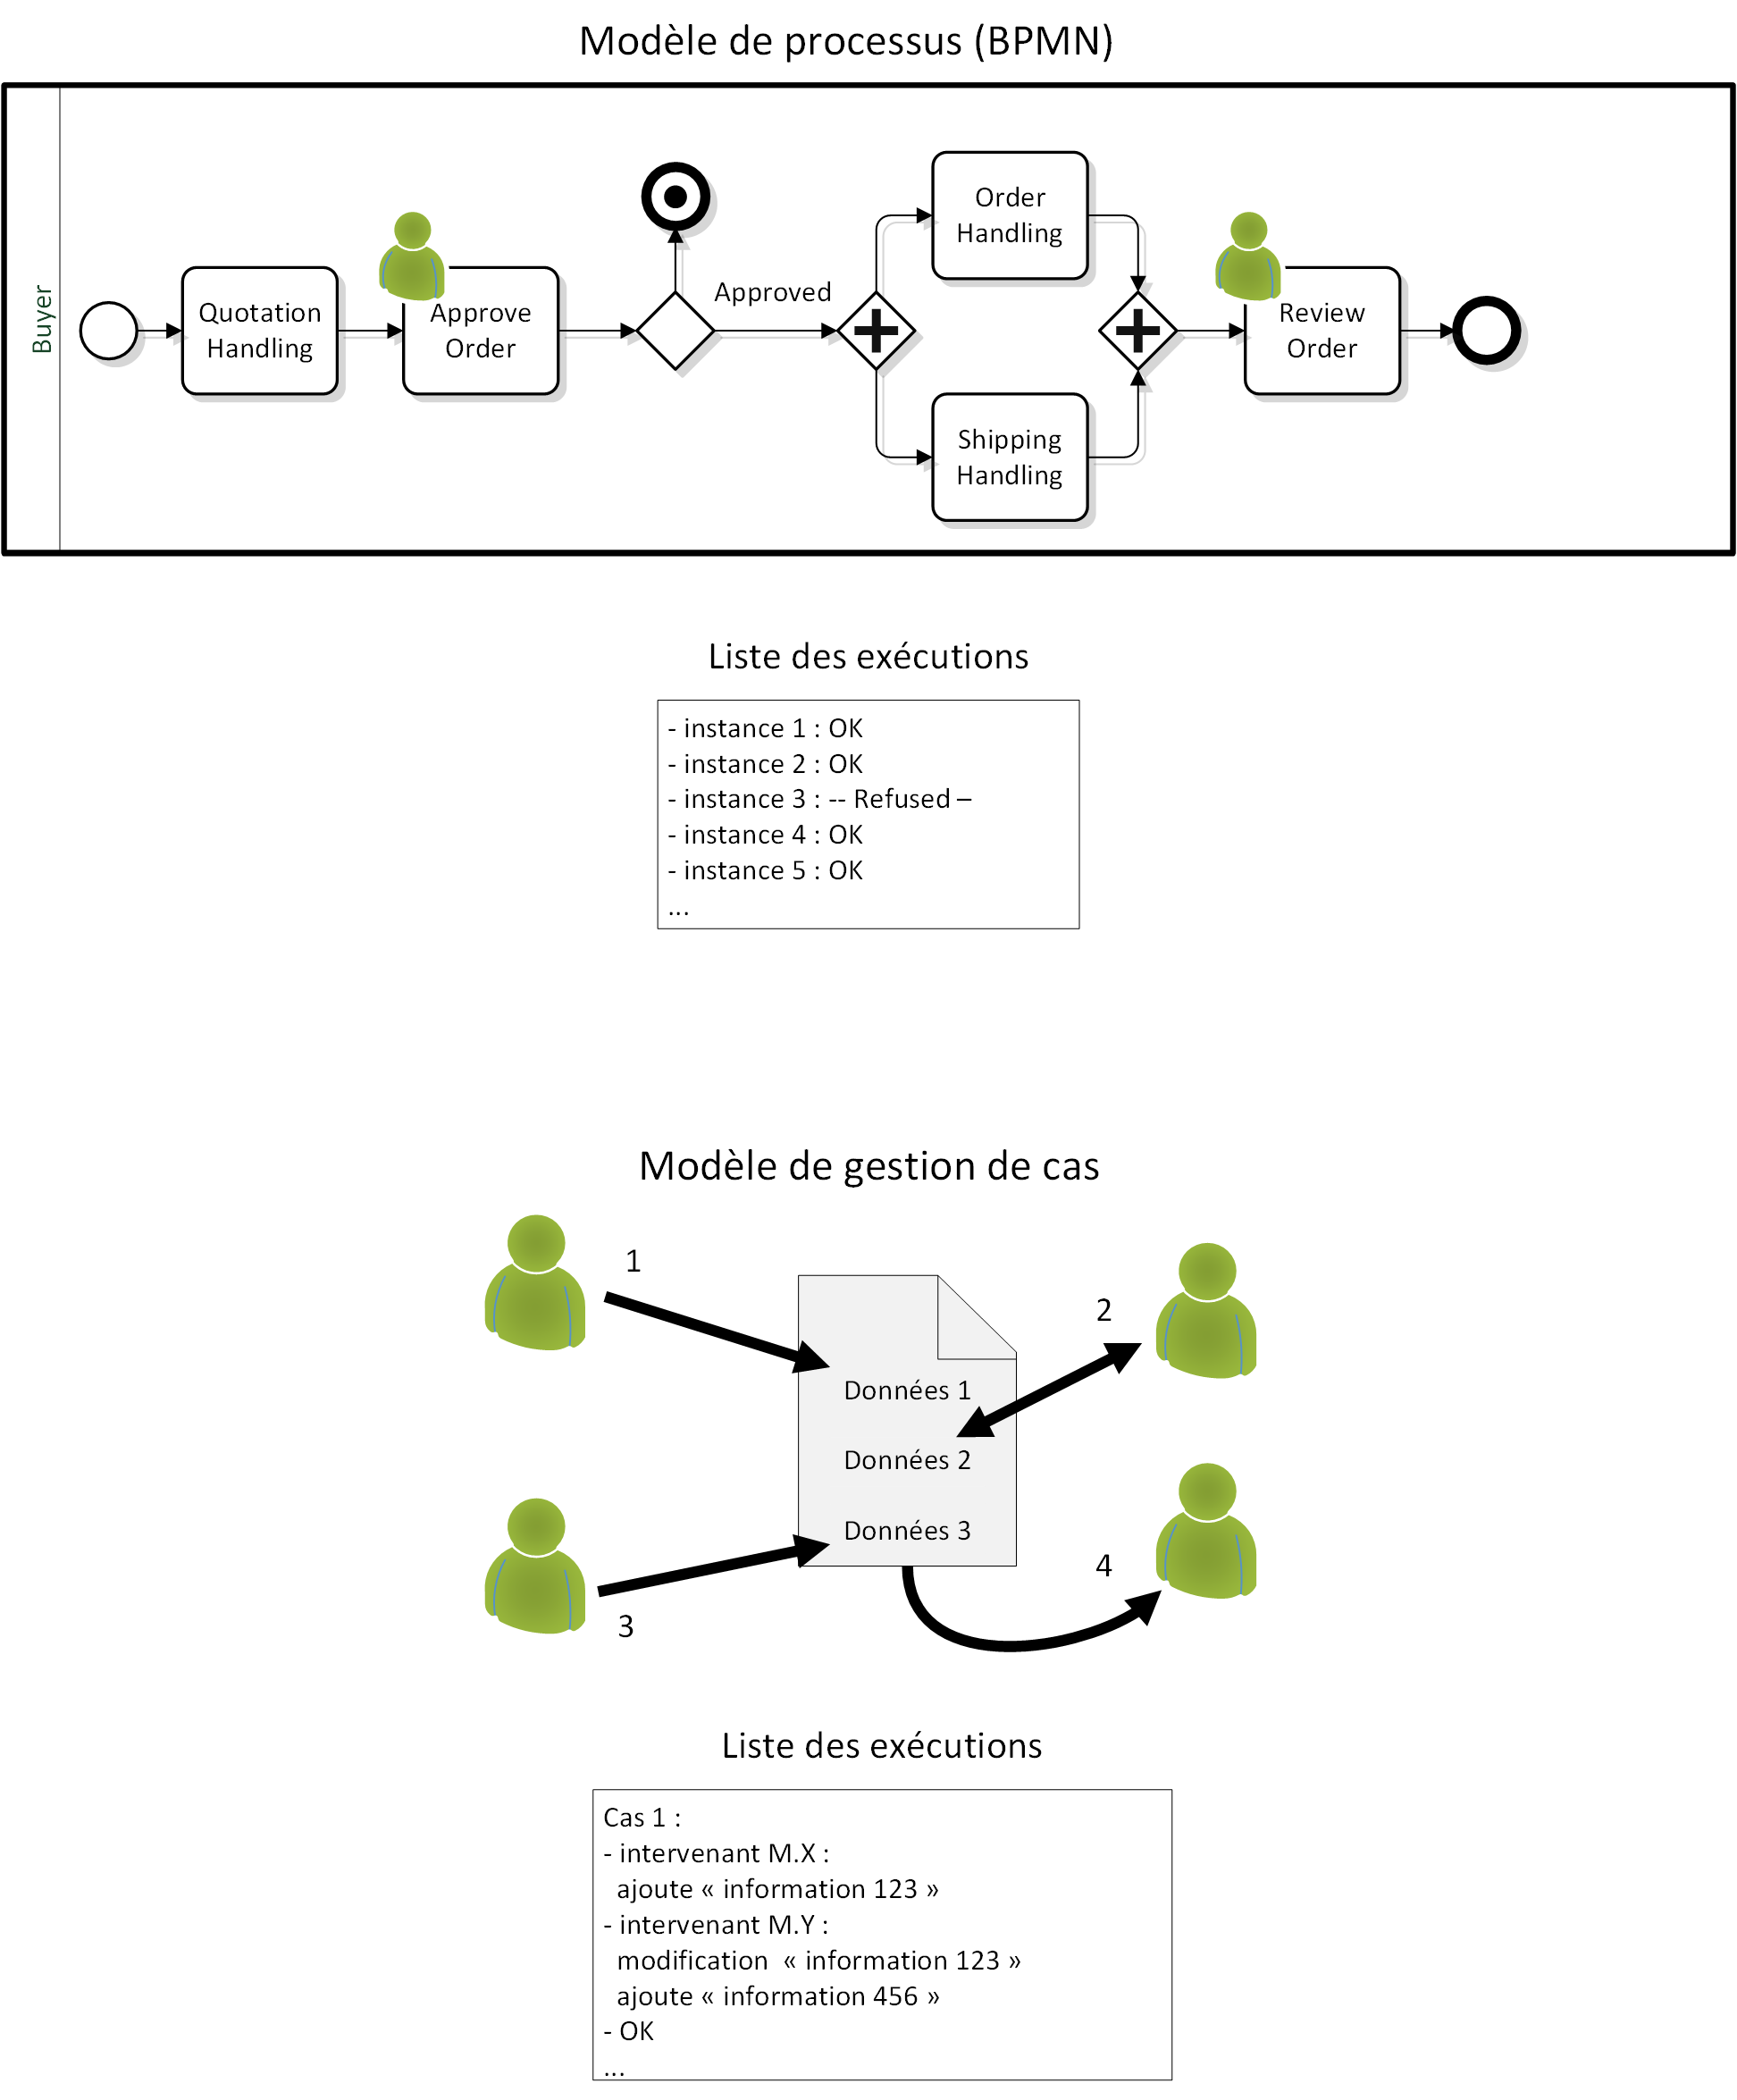
\includegraphics[scale=0.65]{2-Etat-de-l'Art/images/KIP/ACM/Exemple_Cas_vs_BPMN_hauteur.png}
}
\caption{Comparaison des point de vues impératif (BPMN) et gestion de cas}
\label{figure:2-S1-KIP-Exemple-ACM}
\end{figure}


\bigskip

L'ACM est un candidat naturel au traitement des processus à forte intensité de connaissances, de par sa nature à être dirigé par les données et les connaissances, mais également car il s'intéresse aux instances de ces processus, c'est-à-dire les cas.
La différence majeure entre l'ACM et la gestion des connaissances provient du point de vue choisi : il s'agit non pas d'étudier comment les connaissances ou données sont traitées pour en proposer d'autres et les réutiliser, mais bien de traiter des cas et les résoudre grâce à d'anciens cas avec leurs connaissances et données.
L'élément central est le cas, qui sera résolu en s'appuyant sur les connaissances des experts et les données qu'ils produisent et manipulent.
La réutilisation des cas passés, ainsi que des connaissances et données qu'ils embarquent, permet donc de simplifier la gestion des processus à forte intensité de connaissances.





%%%%%%%%%%%%%%%%%%%%%%%%%%%%%%%%%%%%%%%%%%%%%%%%%%%%%%%%%%%%%%%%%%%%%%%%%%%%%%%%%%%%%%%%%%
%%%%%%%%%%%%%%%%%%%%%%%%%%%%%%%%%%%%%%%%%%%%%%%%%%%%%%%%%%%%%%%%%%%%%%%%%%%%%%%%%%%%%%%%%%
%%%%%%%%%%%%%%%%%%%%%%%%%%%%%%%%%%%%%%%%%%%%%%%%%%%%%%%%%%%%%%%%%%%%%%%%%%%%%%%%%%%%%%%%%%
%%%%%%%%%%%%%%%%%%%%%%%%%%%%%%%%%%%%%%%%%%%%%%%%%%%%%%%%%%%%%%%%%%%%%%%%%%%%%%%%%%%%%%%%%%
%%%%%%%%%%%%%%%%%%%%%%%%%%%%%%%%%%%%%%%%%%%%%%%%%%%%%%%%%%%%%%%%%%%%%%%%%%%%%%%%%%%%%%%%%%
%%%%%%%%%%%%%%%%%%%%%%%%%%%%%%%%%%%%%%%%%%%%%%%%%%%%%%%%%%%%%%%%%%%%%%%%%%%%%%%%%%%%%%%%%%

%%%%%%%%%%%%%%%%%%%%%%%%%%%%%%%%%%%%%%%%%%%%
\clearpage % Clean for pictures and tables %
\newpage   % Clean for pictures and tables %
%%%%%%%%%%%%%%%%%%%%%%%%%%%%%%%%%%%%%%%%%%%%

%%%%%%%%%%%%%%%%%%%%%%%%%%%%%%%%%%%%%%%%%%%%%%%%%%%%%%%%%%%%%%%%%%%%%%%%%%%%%%%%%%%%%%%%%%
%%%%%%%%%%%%%%%%%%%%%%%%%%%%%%%%%%%%%%%%%%%%%%%%%%%%%%%%%%%%%%%%%%%%%%%%%%%%%%%%%%%%%%%%%%
%%%%%%%%%%%%%%%%%%%%%%%%%%%%%%%%%%%%%%%%%%%%%%%%%%%%%%%%%%%%%%%%%%%%%%%%%%%%%%%%%%%%%%%%%%
%%%%%%%%%%%%%%%%%%%%%%%%%%%%%%%%%%%%%%%%%%%%%%%%%%%%%%%%%%%%%%%%%%%%%%%%%%%%%%%%%%%%%%%%%%
%%%%%%%%%%%%%%%%%%%%%%%%%%%%%%%%%%%%%%%%%%%%%%%%%%%%%%%%%%%%%%%%%%%%%%%%%%%%%%%%%%%%%%%%%%
%%%%%%%%%%%%%%%%%%%%%%%%%%%%%%%%%%%%%%%%%%%%%%%%%%%%%%%%%%%%%%%%%%%%%%%%%%%%%%%%%%%%%%%%%%


\section{Techniques d'analyse de données}
\label{section:Contexte:TechniquesAnalyseDonnees}

Lors de la construction d'un cours, un enseignant utilise des connaissances implicites, grâce à son expérience personnelle, pour sélectionner les notions enseignées et les enchaîner de façon logique et la plus intuitive possible pour les étudiants.
L'enchaînement de notions étant lui-même un ensemble de connaissances implicites, on constate que la production de connaissances à première vue explicites repose en réalité sur de nombreuses connaissances implicites (à la fois utilisées lors du processus de création, et dans la production finale).
La réutilisation implique donc des traitements spécifiques pour analyser les connaissances embarquées dans les processus à forte intensité de connaissances et les documents qui y sont attachés.
Dans cette section, nous présentons plusieurs techniques permettant de traiter ces connaissances et les données sur lesquelles elles s'appuient.


\bigskip

Les documents étant composés de textes en langage naturel, il est tout d'abord nécessaire de les analyser avec des techniques adaptées issues du domaine du \textit{traitement automatique du langage}.
Une fois les textes analysés, et leur contenu extraits, on peut y rechercher des connaissances implicites grâce à l'\textit{analyse de concepts formels} et deux \textit{métriques dédiées}.
Une première métrique (l'\textit{impact mutuel}) permet d'estimer la pertinence des documents insérés en entrées, tandis qu'une autre (la \textit{similarité conceptuelle}) est utilisée pour construire des \textit{clusters} de termes.
Ces clusters représentent les séances sous forme d'ensemble de notions les plus proches selon les connaissances implicites exploitées par l'analyse de concepts formels.


\bigskip


\subsection{Traitement Automatique du Langage}
\label{subsection:Contexte:TechniquesUtilisees:TAL}

Comme nous l'avons vu, l'une des spécificités des KIP est de manipuler (ou faire intervenir de façon plus subtile) des connaissances, tout comme ACM se concentre sur les données des cas.
Ces connaissances et données se transmettent par des signes et des langages étudiés par plusieurs domaines comme la sémiologie ou sémiotique~\cite{goosse2016bon}.
L'approche présentée dans cette thèse visant en particulier l'enseignement supérieur, donc des activités proprement humaines où les textes sont prédominants, nous faisons appel au domaine du \textit{traitement automatique du langage} (TAL), ou \textit{natural language processing} (NLP) en anglais.
Le "\textit{triangle sémiotique (le terme, le concept, l'objet)}"~\cite{zargayouna2015recherche} propose un point de vue où le texte (composé de termes) exprime par une vue de l'esprit (les concepts) les choses et phénomènes (les objets) observés, ce qui correspond à ce qu'un travailleur du savoir exprimerait dans les documents par rapport à ce qu'il observe ou fait.
Les travaux de cette thèse utilisent le mot \textit{terme} pour désigner la représentation textuelle d'un concept (\og \textit{unit of thought} \fg~\cite{ISO-25964-1}, une unité de la pensée) comme décrit dans la norme ISO 25964-1~\cite{ISO-25964-1}\cite{LivreBlancISO25964-1}.
Un \textit{terme} correspond donc à un ou plusieurs mots, par exemple "\textit{base de données}" est un \textit{terme} composé de trois \textit{mots}.
Dans le domaine particulier de l'enseignement, nous emploierons \textit{notions} ou \textit{sujets} pour parler des unités enseignées aux étudiants.

\bigskip

Afin de manipuler les mêmes \textit{termes} dans l'ensemble des documents traités, il est nécessaire de comprendre les concepts et standardiser leurs représentations textuelles.
Pour cela, nous employons une succession d'outils pour effectuer l'étiquetage morpho-syntaxique des mots, puis désambiguïser le sens et les lier aux \textit{entités} d'une base de connaissances.
Les \textit{termes} sont donc les signifiants des concepts (signifiés) contenus dans les bases de connaissances.

\bigskip

Certaines classes grammaticales de mots ne permettant pas de déterminer des notions que nous souhaitons réutiliser, il est nécessaire de les filtrer.
L'étiquetage morpho-syntaxique, ou \textit{part-of-speech tagging} (POS tagging) en anglais, permet de déterminer la classe grammaticale des mots~\cite{voutilainen2003part}\cite{agirre2007word}.
La plupart des étiqueteurs découpent tout d'abord les textes en tokens en détectant la ponctuation ou d'autres limites de fin de mot, puis recherchent les ambiguïtés en comparant les mots reconnus et leurs formes dans un lexique (les articles sont immédiatement détectables comparés aux noms et verbes dont les formes changent et peuvent induire des ambiguïtés : \textit{restes} peut désigner un nom ou un verbe), enfin les mots ambigües sont analysés pour déterminer la classe la plus probable~\cite{voutilainen2003part}.
Pour étiqueter les mots et supprimer ceux ne portant pas de concepts utiles, par exemple les articles ou prépositions, nous utilisons TreeTagger~\cite{schmid1994probabilistic}\cite{Schmid95improvementsin}.
Celui-ci repose sur des arbres de décision pour déterminer la classe grammaticale la plus probable en fonction du contexte.

\bigskip

Afin de retrouver les termes ainsi que les notions qui leurs sont rattachées, il est nécessaire d'utiliser un outil désambiguïsant les mots, ou \textit{word sense disambiguation} (WSD) en anglais, puis faisant les liens avec les entités nommées, ou \textit{entity linking} (EL) en anglais.
L'annotation sémantique est une famille de techniques de TAL permettant d'identifier des entités nommées dans des textes, et de les lier aux entités d'une base de connaissances~\cite{rao2013entity}.
Ces techniques font partie du domaine de l'extraction d'informations qui permet le stockage et la réutilisation de ces connaissances à partir de textes en langue naturelle~\cite{rao2013entity}.
Afin de reconnaître ces entités, et éventuellement leurs synonymes, une étape de désambiguïsation des mots est requise.
Nous avons opté pour BabelFy~\cite{moro2014entity}\cite{moro2014multilingual}, un outil de désambiguïsation et d'annotation sémantique, lié à BabelNet~\cite{navigli2012babelnet}, un réseau sémantique multilingue manipulant des concepts et des entités nommées lui-même lié à WordNet~\cite{miller1995wordnet} et Wikipedia~\cite{volkel2006semantic}\cite{merzeau2015wikipedia}.

\bigskip

L'usage de Wikipedia comme base de connaissances peut paraitre déraisonnable scientifiquement de par la qualité de certains articles, mais celle-ci étant la plus grande base de connaissances collaborative et multilingue~\cite{navigli2012babelnet}, il devient possible d'exploiter des entités nommées de la vie courante (par exemple des personnalités publiques, des marques, ou encore des entreprises).
Dans~\cite{bunescu-pasca-2006-using} il est également présenté comment l'usage de Wikipedia améliore les résultats de la désambiguïsation des entités nommées par rapport à des encyclopédies moins complètes.
La quantité d'articles, de langues, l'aspect collaboratif permettant de la maintenir à jour avec une cohérence vis-à-vis des évènements quotidiens, et sa simplicité la rendent particulièrement adaptée pour cette tâche.

\bigskip

Les travaux présentés dans~\cite{navigli2012babelnet} visent à construire un réseau sémantique multilingue nommé BabelNet.
Un réseau sémantique sert à représenter des concepts exprimés par des mots du langage naturel et des phrases sous forme de n\oe{}uds reliés par des arcs représentants les relations sémantiques entre eux~\cite{simmons1972semantic}.
L'approche utilisée pour BabelNet consiste à lier la plus grande encyclopédie multilingue (Wikipedia) au lexique informatisé le plus populaire (WordNet)~\cite{navigli2012babelnet}.
Les entités de Wikipedia sont automatiquement liées aux mots et expressions stockés dans WordNet dans plusieurs langues.
Les entités non liées, ou dont les traductions sont manquantes, sont ensuite traitées avec des outils de traduction automatique, ou \textit{Machine Translation} en anglais, sur des ensembles de données issus de Wikipedia et SemCor~\cite{miller1993semantic}.
Le réseau sémantique ainsi créé est un des plus performants~\cite{navigli2012babelnet}.

\bigskip

Afin de comprendre les unités manipulées par BabelNet, il est nécessaire de décrire succinctement WordNet.
WordNet~\cite{miller1995wordnet} est une base de données lexicale initialement dédiée à l'anglais, mais étendue à quelques autres langues, qui manipule les concepts à l'aide de \textit{synsets} (\textit{synonym set}, un ensemble de synonymes)~\cite{navigli2012babelnet}.
En l'interrogeant sur un mot, celle-ci renvoie chaque synset disposant du mot en précisant les sens et les classes grammaticales associées.
Lorsque BabelNet est interrogé sur un concept au travers du (ou des) mot(s) le représentant, celui-ci renvoie également un synset (appelé dans ce cas un \textit{Babel synset}) en précisant l'article Wikipedia associé à l'entité nommée et éventuellement le synset WordNet lorsque celui-ci existe.
Afin d'obtenir l'équivalent du (ou des) mot(s) dans d'autres langues, les traductions proposées par Wikipedia sont collectées et liées aux Babel synsets, puis les traductions manquantes sont recherchées avec les techniques de traduction automatique dans les corpus de SemCor.
Chaque Babel synset dispose également d'un identifiant unique au format $bn{:}xxxxxxxxY$, où les huit \textit{x} sont des chiffres et \textit{Y} une lettre correspondant à la classe grammaticale.
Ainsi, BabelNet regroupe un ensemble de concepts et d'entités nommées sous forme de Babel synsets composés de mots liés aux entités nommées stockées dans Wikipedia.

\bigskip

L'outil permettant d'extraire les entités nommées d'un texte s'appelle \textit{BabelFy}~\cite{moro2014entity}\cite{moro2014multilingual}.
Celui-ci permet de retrouver les Babel synsets (et leurs identifiants) associés aux concepts et entités manipulés dans le texte.
BabelFy vise à combiner la désambiguïsation des mots (WSD) et la reconnaissance d'entités nommées (EL), afin de retrouver l'ensemble des entités nommées possibles pour chaque mot ou ensemble de mots.
Un morceau de texte peut permettre d'extraire plusieurs entités (les entités nommées et mentions nominales) comme le montre l'exemple dans~\cite{moro2014entity} : pour \og \textit{Major League Soccer} \fg, on retrouve l'entité \textit{Major League Soccer}, mais également les mentions nominales \textit{major league}, \textit{league}, et \textit{soccer}.

Afin de fonctionner, BabelFy construit tout d'abord un ensemble de signatures sémantiques à partir de l'ensemble des concepts et entités nommées du réseau sémantique BabelNet.
Cette opération ne se déroule qu'une seule fois (ou au plus après chaque mise à jour de BabelNet).
Pour chaque texte inséré, son contenu est étiqueté grammaticalement, puis, toutes les suites possibles de un à cinq mots consécutifs contenant au moins un nom (afin de pouvoir se lier à une entité dans BabelNet) sont créées.
Un ensemble d'entités candidates pour chacune de ces suites est constitué.
Les entités candidates de l'ensemble du texte sont réunies dans un graphe où les arcs représentent les signatures candidates entre chaque suite de mots.
Un algorithme retire petit à petit les entités candidates dont les degrés sont les plus faibles, et obtient ainsi un ensemble de candidats fortement liés.
Les entités candidates les moins liées les unes avec les autres, car d'un domaine différent, sont donc supprimées des réponses.
Pour chacune des entités candidates retenues, trois scores sont établis.
Les travaux dans~\cite{prohaska2017masterthesis} les décrivent ainsi :
\begin{itemize}
\item Le \textit{score de désambiguïsation} (\textit{disambiguation score} en anglais) correspond à la confiance établie entre le (ou les) mot(s) d'origine et le Babel synset choisi. Il s'agit du score qu'établirait une étape de désambiguïsation des mots (WSD) seule, c'est-à-dire si la création de lien vers des entités nommées (EL) n'était pas effectuée en même temps.
\item Le \textit{score de cohérence} (\textit{coherence score} en anglais) correspond au degré de connexion du Babel synset retenu par rapport aux autres Babel synset dans le graphe final représentant le texte inséré.
\item Le \textit{score de pertinence} (\textit{relevant score} en anglais) correspond à la pertinence du concept dans le texte inséré. Celui-ci est calculé uniquement selon la position du n\oe{}ud dans le graphe, sans que cela ne soit lié au Babel synset.
\end{itemize}

\bigskip

Pour le cas de l'enseignement supérieur, ces techniques permettent donc de lire les supports de cours et d'en extraire les notions abordées, c'est-à-dire les entités nommées qui les composent.
Ces entités nommées étant standardisées au moyen des bases de connaissances utilisées par BabelFy et BabelNet, il est possible de chercher des points communs entre les documents insérés.


\bigskip

%%%%%%%%%%%%%%%%%%%%%%%%%%%%%%%%%%%%%%%%%%%%
%\clearpage % Clean for pictures and tables %
%\newpage   % Clean for pictures and tables %
%%%%%%%%%%%%%%%%%%%%%%%%%%%%%%%%%%%%%%%%%%%%

\subsection{Analyse de Concepts Formels}
\label{subsection:Contexte:TechniquesUtilisees:ACF}

L'\textit{Analyse de Concepts Formels} (ACF)~\cite{wille1982restructuring}\cite{wille2005formal}, ou \textit{Formal Concept Analysis} (FCA) en anglais, est une méthode d'analyse de données.
Elle permet d'analyser des données décrivant les relations entre des objets et leurs attributs~\cite{belohlavek2008introduction} en \og \textit{visualisant les structures, implications, et dépendances inhérentes} \fg~\cite{wormuth2004introduction}.
Ces objets et leurs attributs sont rassemblés dans un \textit{treillis} composé de \textit{concepts formels}, c'est-à-dire un graphe avec des propriétés particulières.
La notion de \textit{concepts formels} n'est pas totalement étrangère à la définition présentée dans la sous-section précédente, principalement car l'ACF peut aussi être définie comme une \og \textit{mathématisation de la compréhension philosophique des concepts} \fg (\og \textit{is a mathematization of the philosophical understanding of concept} \fg~\cite{wormuth2004introduction}).
En effet, d'après~\cite{belohlavek2008introduction}, l'objectif de l'ACF est de pouvoir décrire des \textit{concepts} humains sous forme de \textit{concepts formels} tels que \og voiture à quatre roues motrices \fg ou \og nombres divisibles par 3 et 4 \fg, afin d'en déduire des implications telles que \og tous les nombres divisibles par 3 et 4 sont divisibles par 6 \fg.
Des liens avec d'autres domaines de recherche sont également présentés par l'un des fondateurs de l'ACF dans~\cite{wille2005formal}.
Du point de vue du \textit{treillis} (pouvant être considéré comme un graphe), un \textit{concept formel} est un n\oe{}ud contenant simultanément un ensemble d'objets, et un ensemble d'attributs.

Dans le cadre de cette thèse, l'ACF va donc permettre de manipuler les notions issues des documents (représentées par les termes récupérés avec l'aide des techniques de TAL) pour les analyser et en extraire des implications.
Précisément, nous analysons les termes en tant qu'objets, et les supports de cours où ils apparaissent en tant qu'attributs.

\bigskip

\subsubsection{Stratégies de binarisation}
\label{subsubsection:Contexte:ACF-StrategiesBinarisation}

L'ACF repose sur un treillis de Galois sur lequel diverses interprétations sont effectuées pour découvrir des connaissances~\cite{jaffal2019aide}.
Pour construire ce treillis, il est nécessaire de fournir un \textit{contexte formel} rassemblant les liens entre les objets et leurs attributs.
Le \textit{contexte formel} étant une matrice binaire, il est nécessaire d'appliquer une transformation lorsque les données analysées forment une matrice multivaluée.
Dans le cas de l'enseignement supérieur, les matrices sont constituées d'occurrences de termes dans des supports de cours, donc de valeurs pouvant être supérieures à $ 1 $.
Une stratégie de binarisation définit un algorithme qui transforme les valeurs d'une matrice de l'intervalle $ [0, +\infty [ $ vers la paire $ \{ 0, 1 \} $.

\bigskip

Il existe actuellement plusieurs stratégies pour permettre à l'ACF de présenter différentes informations contenues dans une matrice multivaluée~\cite{jaffal2015refinement}\cite{jaffal2019aide}.
Nous pouvons citer les stratégies les plus évidentes que sont les stratégies dites \textit{directe} et \textit{inverse} :

\begin{enumerate}
\item Stratégie Directe : il s'agit de la stratégie la plus simple, les valeurs non-nulles sont remplacées par des 1, et les valeurs nulles sont remplacées par des 0.
L'objectif est simplement de montrer les liens entre les objets et attributs sans aucune pondération.
Dans notre cas, on peut donc voir quels termes sont présents dans quels documents.\\

\item Stratégie Inverse : il s'agit de la stratégie inverse à la stratégie directe, les valeurs non-nulles sont remplacées par des 0, et les valeurs nulles sont remplacées par des 1.
L'objectif est de montrer la matrice inverse (d'où son nom) et les relations engendrées entre les objets et attributs.
Dans notre cas, on peut donc voir quels termes sont absents dans quels documents.
\end{enumerate}

\bigskip

Les stratégies directe et inverse sont illustrées en figure~\ref{figure:2-S2-Exemple-Strategies-Simples}, on notera que les stratégies peuvent être simplifiées en supprimant les lignes et colonnes ne contenant que des 0.
Bien que ces stratégies semblent triviales, la stratégie directe est néanmoins utile pour exposer des informations concernant les termes les plus importants ainsi que la pertinence des documents insérés comme nous le verrons plus tard en sous-section~\ref{subsection:CREA:PII.2-GrapheImpactMutuel}.


%\begin{figure*} % Figure flottante
\begin{figure}[ht]
\centering
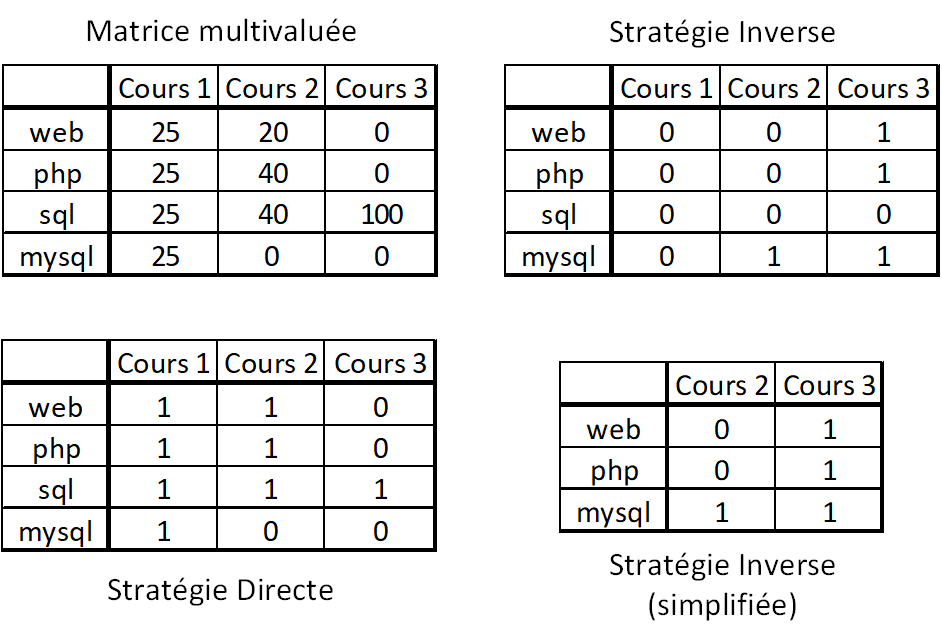
\includegraphics[scale=1]{2-Etat-de-l'Art/images/ACF/Strategies/exemple_strategies_simples.png}
\caption{Exemple d'application des stratégies directe et inverse}
\label{figure:2-S2-Exemple-Strategies-Simples}
\end{figure}
%\end{figure*} % Figure flottante
% To use it : fig~\ref{label}

\bigskip

Trois autres stratégies prenant en compte la pondération sont aussi présentées dans~\cite{jaffal2015refinement}\cite{jaffal2019aide}.
Celles-ci se basent sur la prise en compte de \textit{l'intensité de la relation entre chaque objet et chaque attribut, via le calcul d'une valeur de fréquence}~\cite{jaffal2019aide}.
Deux seuils sont fixés par un $ \beta \in [0, 1] $.
Les seuils sont équidistants de la valeur $ 0,5 $ (indiquée par la ligne en pointillés rouges) et s'en éloignent au fur et à mesure que $ \beta $ augmente, comme illustré sur la figure~\ref{figure:2-S2-Strategies-Exemple-Seuils}.
Ces seuils permettent de découper l'espace entre $ 0 $ et $ 1 $ en trois parties : les valeurs de fréquences hautes (au dessus du \textit{seuil haut}) associées à la \textit{stratégie à haute dépendance}, les valeurs de fréquences basses (en dessous du \textit{seuil bas}) associées à la \textit{stratégie à faible dépendance}, et les valeurs de fréquences moyennes (entre les \textit{seuil haut} et \textit{seuil bas}) associées à la \textit{stratégie à dépendance moyenne}.

La figure~\ref{figure:2-S2-Strategies-Exemple-Trois-Parties} présente plusieurs exemples suivant les valeurs de $ \beta $.
On notera que lorsque $ \beta $ vaut $ 0 $, il n'y a qu'un seuil à $ 0,5 $ découpant l'espace en seulement deux parties (les valeurs à fréquences hautes et basses), et inversement, lorsque $ \beta $ vaut $ 1 $, les deux seuils sont à $ 0 $ et $ 1 $ découpant l'espace en seulement une partie (les valeurs à fréquences moyennes).

%\begin{figure*} % Figure flottante
\begin{figure}[ht]
\centering
\centerline{
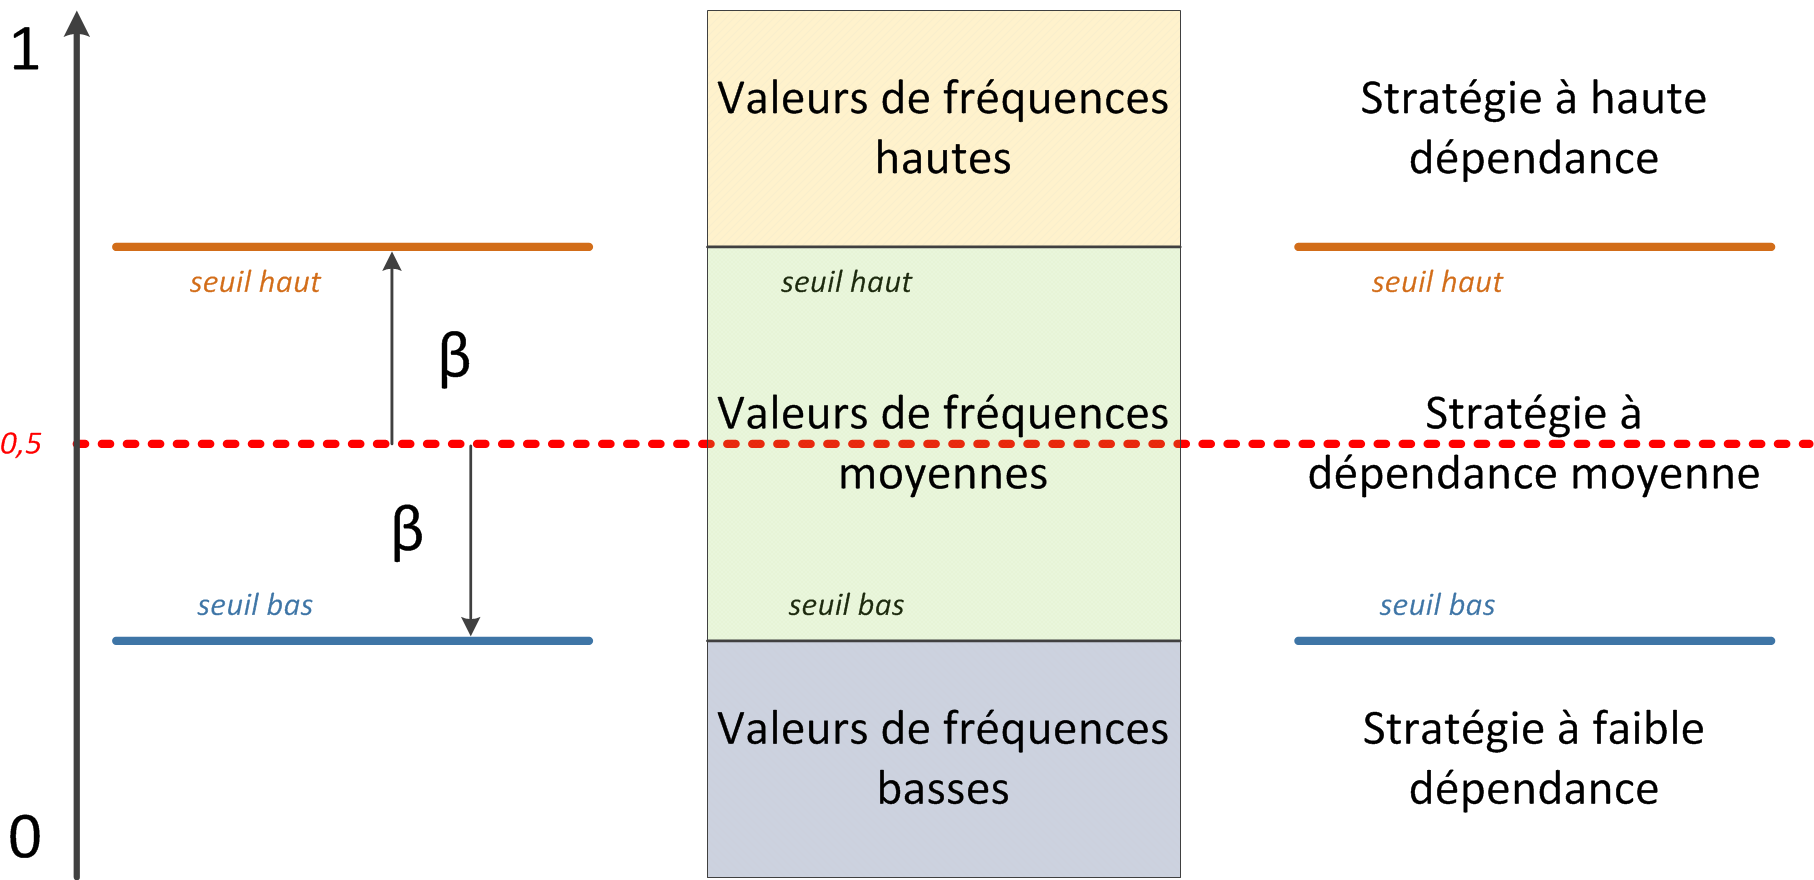
\includegraphics[scale=0.65]{2-Etat-de-l'Art/images/ACF/Strategies/explication_strategies_seuils_beta.png}
}
\caption{Les deux seuils générés par $ \beta $ découpent l'espace en trois parties}
\label{figure:2-S2-Strategies-Exemple-Seuils}
\end{figure}
%\end{figure*} % Figure flottante
% To use it : fig~\ref{label}

%\begin{figure*} % Figure flottante
\begin{figure}[ht]
\centering
%\includegraphics[width=3in]{images/VerySmallModels_text.png}
%%\includegraphics[scale=0.6]{images/VerySmallModels_text.png}
\centerline{  % FORCE FIGURE OUTSIDE THE MARGIN !!! BUT STILL CENTERING !!!
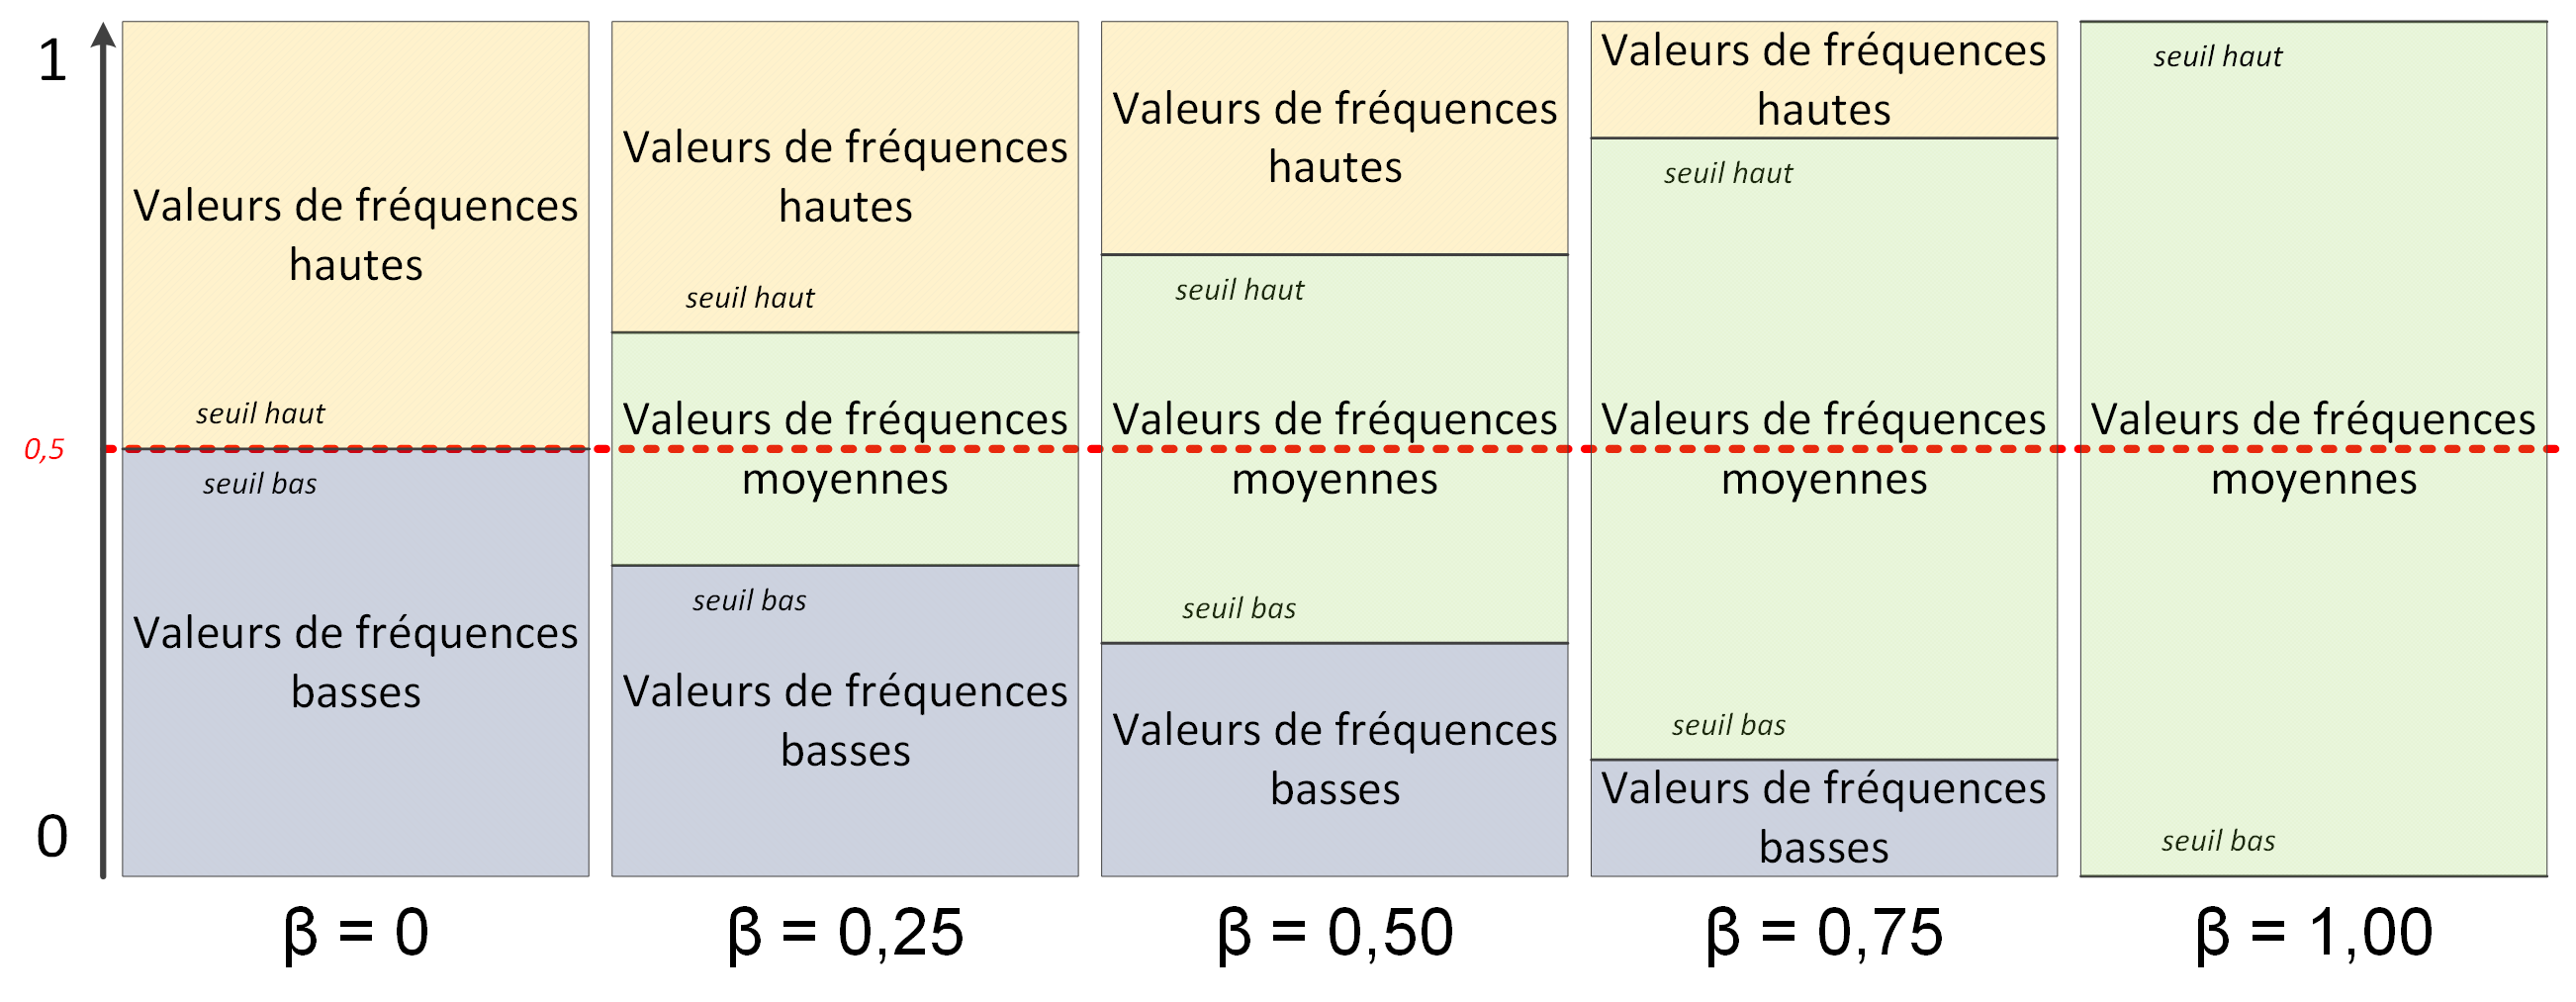
\includegraphics[scale=0.6]{2-Etat-de-l'Art/images/ACF/Strategies/explication_strategies_trois_parties.png}
}
\caption{Différentes valeurs de $ \beta $ séparent l'espace en plusieurs parties}
\label{figure:2-S2-Strategies-Exemple-Trois-Parties}
\end{figure}
%\end{figure*} % Figure flottante
% To use it : fig~\ref{label}

\bigskip

Selon le $ \beta $ choisi, les seuils vont se fixer pour permettre de délimiter les bornes des valeurs de fréquences requises pour chaque stratégie.
Ensuite, la formule~\eqref{equation:2-S2-Strategies-Frequence} permet d'obtenir la valeur de fréquence pour chaque proportion d'occurrences d'un terme dans un document de la matrice fournie.
La valeur de fréquence ainsi obtenue est transformée en $ 0 $ ou $ 1 $ selon son positionnement entre les seuils (et donc par rapport à la stratégie sélectionnée).
Les seuils hauts et bas sont positionnés en suivant les formules~\eqref{equation:2-S2-Strategies-Seuil-Haut} et~\eqref{equation:2-S2-Strategies-Seuil-Bas}.
La matrice multivaluée est ainsi transformée en matrice binaire qui peut être utilisée comme un \textit{contexte formel} par la suite.
Afin de générer une matrice binaire, il faut donc fixer un $ \beta $ et sélectionner une stratégie parmi les suivantes :
\begin{itemize}
\item La \textit{stratégie à haute dépendance} contient les termes dont la valeur de fréquence est supérieure au seuil haut.
Il s'agit des termes qui apparaissent les plus fréquemment dans l'ensemble des documents.
\item La \textit{stratégie à faible dépendance} contient les termes dont la valeur de fréquence est inférieure au seuil bas.
Il s'agit des termes qui apparaissent les moins fréquemment dans l'ensemble des documents.
\item La \textit{stratégie à dépendance moyenne} contient les termes dont la valeur de fréquence est inférieure au seuil haut tout en étant supérieure au seuil bas.
Il s'agit des termes qui apparaissent ni trop fréquemment ni trop rarement dans l'ensemble des documents.
\end{itemize}

\begin{equation}
\text{\textit{fréquence}}(T, D) = \frac{\text{\textit{Nb d'occurrences du terme T dans le document D}}}{\text{\textit{Nb d'occurrences du terme T dans tous les documents}}}
\label{equation:2-S2-Strategies-Frequence}
\end{equation}

\begin{equation}
\text{\textit{seuil haut}} = \text{\textit{Moyenne des fréquences}} + \beta \times \text{\textit{Écart type des fréquences}}
\label{equation:2-S2-Strategies-Seuil-Haut}
\end{equation}

\begin{equation}
\text{\textit{seuil bas}} = \text{\textit{Moyenne des fréquences}} - \beta \times \text{\textit{Écart type des fréquences}}
\label{equation:2-S2-Strategies-Seuil-Bas}
\end{equation}

\bigskip

La figure~\ref{figure:2-S2-Strategies-Exemple-Beta} illustre ces trois stratégies avec un $ \beta $ fixé à 0,50.
On remarque que les valeurs non nulles de chaque ligne sont distribuées dans chacune des stratégies : \textit{web} et \textit{php} voient leurs deux valeurs non nulles distribuées dans les stratégies basses et hautes, \textit{sql} voit ses trois valeurs distribuées dans toutes les stratégies, tandis que \textit{mysql} a son unique valeur non nulle rattachée à la stratégie moyenne.

%\begin{figure*} % Figure flottante
\begin{figure}[ht]
\centering
\centerline{  % FORCE FIGURE OUTSIDE THE MARGIN !!! BUT STILL CENTERING !!!
% scale = 0.6
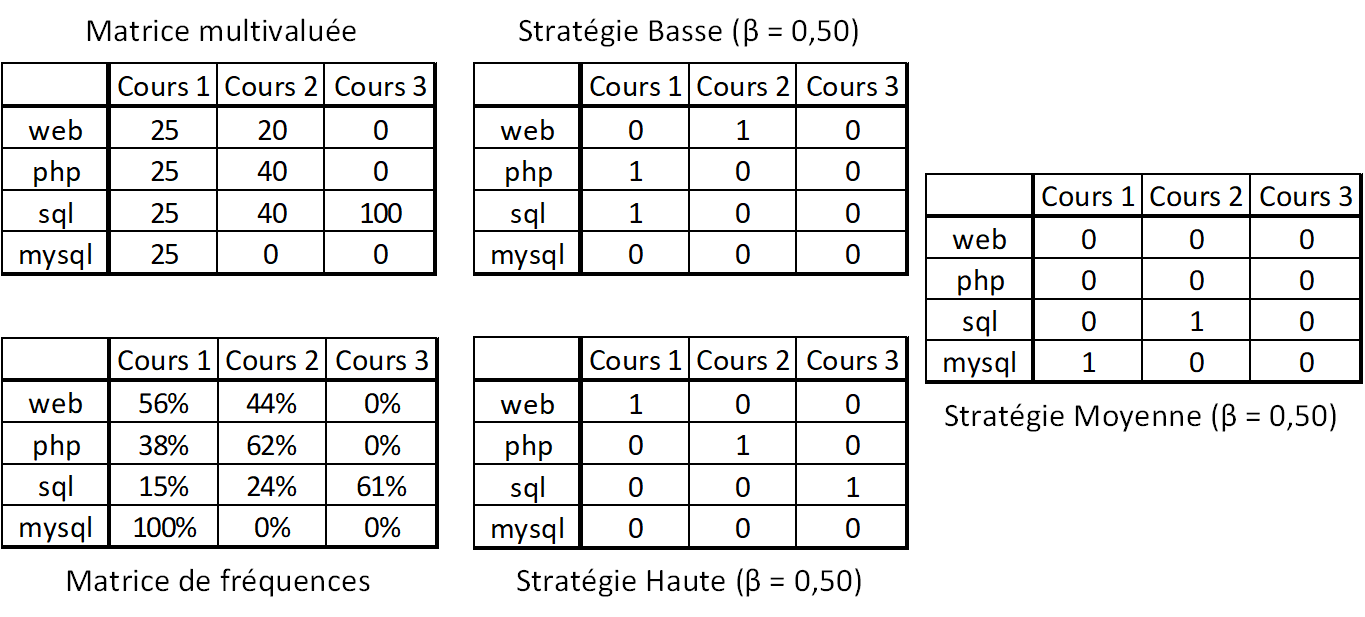
\includegraphics[scale=1]{2-Etat-de-l'Art/images/ACF/Strategies/exemple_strategies_beta=0.50.png}
}
\caption{Exemple d'application des stratégies complexes avec un $ \beta = 0,50 $}
\label{figure:2-S2-Strategies-Exemple-Beta}
\end{figure}
%\end{figure*} % Figure flottante
% To use it : fig~\ref{label}



\bigskip
%\newpage % esthétique

%%%%%%%%%%%%%%%%%%%%%%%%%%%%%%%%%%%%%%%%%%%%
%\clearpage % Clean for pictures and tables %
%\newpage   % Clean for pictures and tables %
%%%%%%%%%%%%%%%%%%%%%%%%%%%%%%%%%%%%%%%%%%%%

\subsubsection{Construction du treillis de Galois (PII.1.d) :}
\label{subsubsection:Contexte:ACF-ConstructionTreillis}

Le \textit{contexte formel} généré avec les stratégies de binarisation contient maintenant des termes liés à des documents par des $ 0 $ et des $ 1 $.
Il peut maintenant être transformé en un \textit{treillis de Galois} pour en extraire des \textit{concepts formels} qui serviront de \textit{fragments} (de cas passés) réutilisables.

\bigskip

La construction d'un treillis de Galois depuis un contexte formel peut se réaliser avec plusieurs algorithmes~\cite{messai2009analyse}.
Chaque n\oe{}ud du treillis correspond à un \textit{concept formel}.
Un \textit{concept formel} contient le maximum d'objets partageant un maximum d'attributs communs, c'est-à-dire que le maximum de termes sont rassemblés selon le maximum de documents auxquels ils sont liés.
La figure~\ref{figure:2-S2-Treillis-Construction-Treillis} illustre le treillis de Galois issu d'un contexte formel (une version simplifiée du contexte formel est présente, afin de mieux observer les résultats sur le treillis).
Les concepts formels aux deux extrémités haute et basse du treillis contiennent respectivement l'ensemble des objets (avec éventuellement le(s) attribut(s) commun(s) à tous les objets) et l'ensemble des attributs (avec éventuellement le(s) objet(s) commun(s) à tous les attributs).

%\begin{figure*} % Figure flottante
\begin{figure}[ht]
\centering
\centerline{  % FORCE FIGURE OUTSIDE THE MARGIN !!! BUT STILL CENTERING !!!
% scale = 0.8
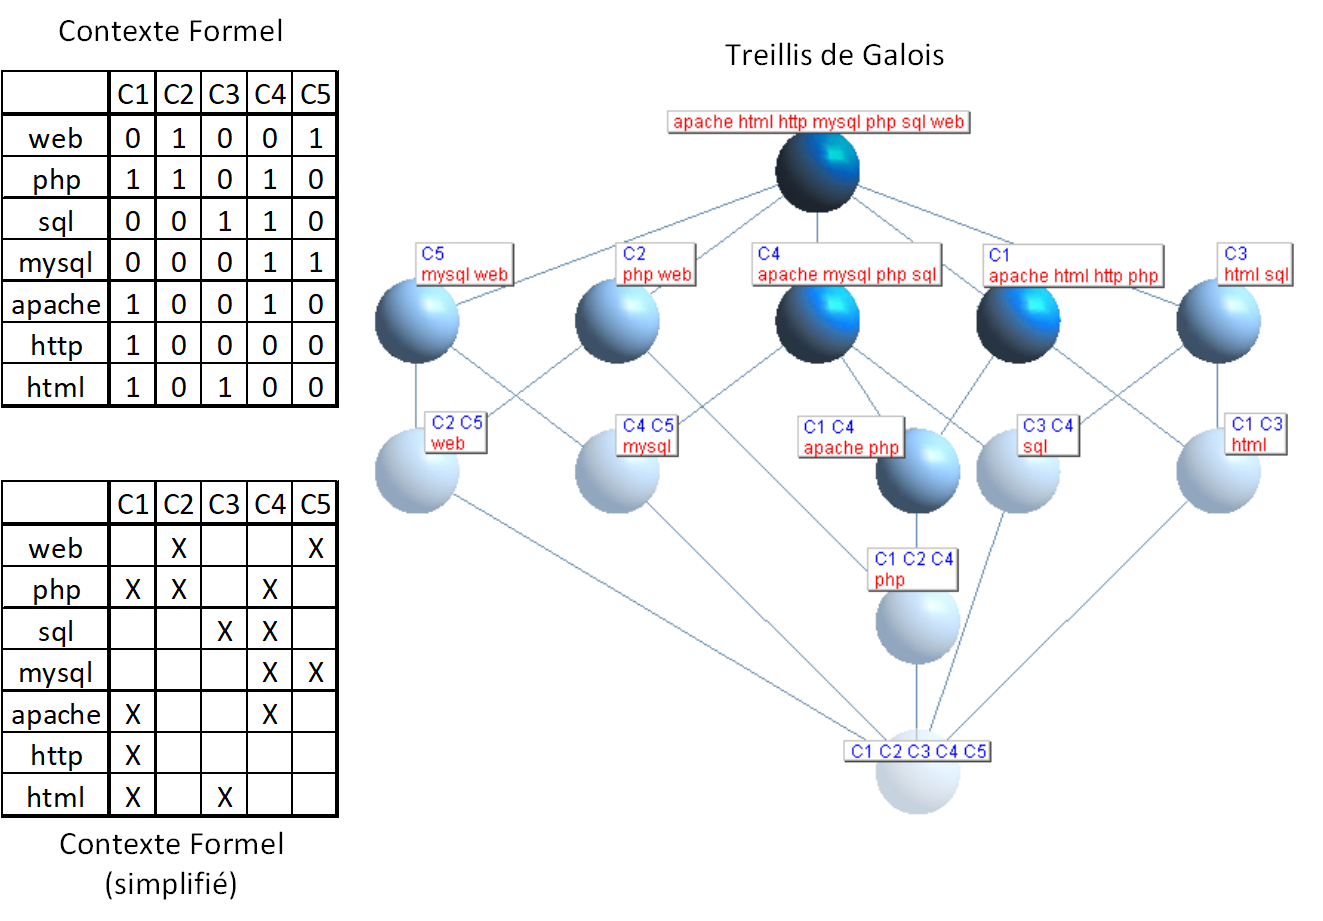
\includegraphics[scale=1]{2-Etat-de-l'Art/images/ACF/Treillis/exemple_treillis_ExampleMediumMatrix-S-B-B-0.00.png}
}
\caption{Contexte formel et son treillis de Galois}
\label{figure:2-S2-Treillis-Construction-Treillis}
\end{figure}
%\end{figure*} % Figure flottante
% To use it : fig~\ref{label}

\bigskip

Dans l'exemple, nous retrouvons donc l'ensemble des termes du contexte formel (qui ne partagent aucun document commun) dans le concept formel du haut, et l'ensemble des documents (qui ne partagent aucun terme commun) dans le concept formel du bas.
En partant du concept formel contenant tous les objets, chaque attribut non nul du contexte formel est progressivement ajouté pour former le plus grand sous-ensemble d'objets.
Chaque niveau du treillis introduit ainsi un attribut supplémentaire (certains niveaux peuvent être vides).
Dans notre exemple, nous voyons au niveau 0 l'ensemble des termes "\textit{apache}", "\textit{html}", "\textit{http}", "\textit{mysql}", "\textit{php}", "\textit{sql}", et "\textit{web}", puis au niveau 1, un document est ajouté à chaque concept formel pour former le sous-ensemble le plus grand de termes partageant cet attribut commun : "\textit{apache}", "\textit{mysql}", "\textit{php}", et "\textit{sql}" ont le document "\textit{C4}" en commun, mais "\textit{apache}", "\textit{html}", "\textit{http}", et "\textit{php}" ont le document "\textit{C1}" en commun.
En niveau 2, un sous-ensemble plus restreint de termes possède deux documents en commun : "\textit{apache}" et "\textit{php}" partagent les documents "\textit{C1}" et "\textit{C4}".
Ensuite, au niveau 3, seul le terme "\textit{php}" est partagé par trois documents "\textit{C1}", "\textit{C2}", et "\textit{C4}".
Finalement, au niveau 4, les cinq documents du contexte formel sont réunis en un concept formel sans aucun terme.

%\begin{figure*} % Figure flottante
\begin{figure}[ht]
\centering
\centerline{  % FORCE FIGURE OUTSIDE THE MARGIN !!! BUT STILL CENTERING !!!
% scale = 0.7
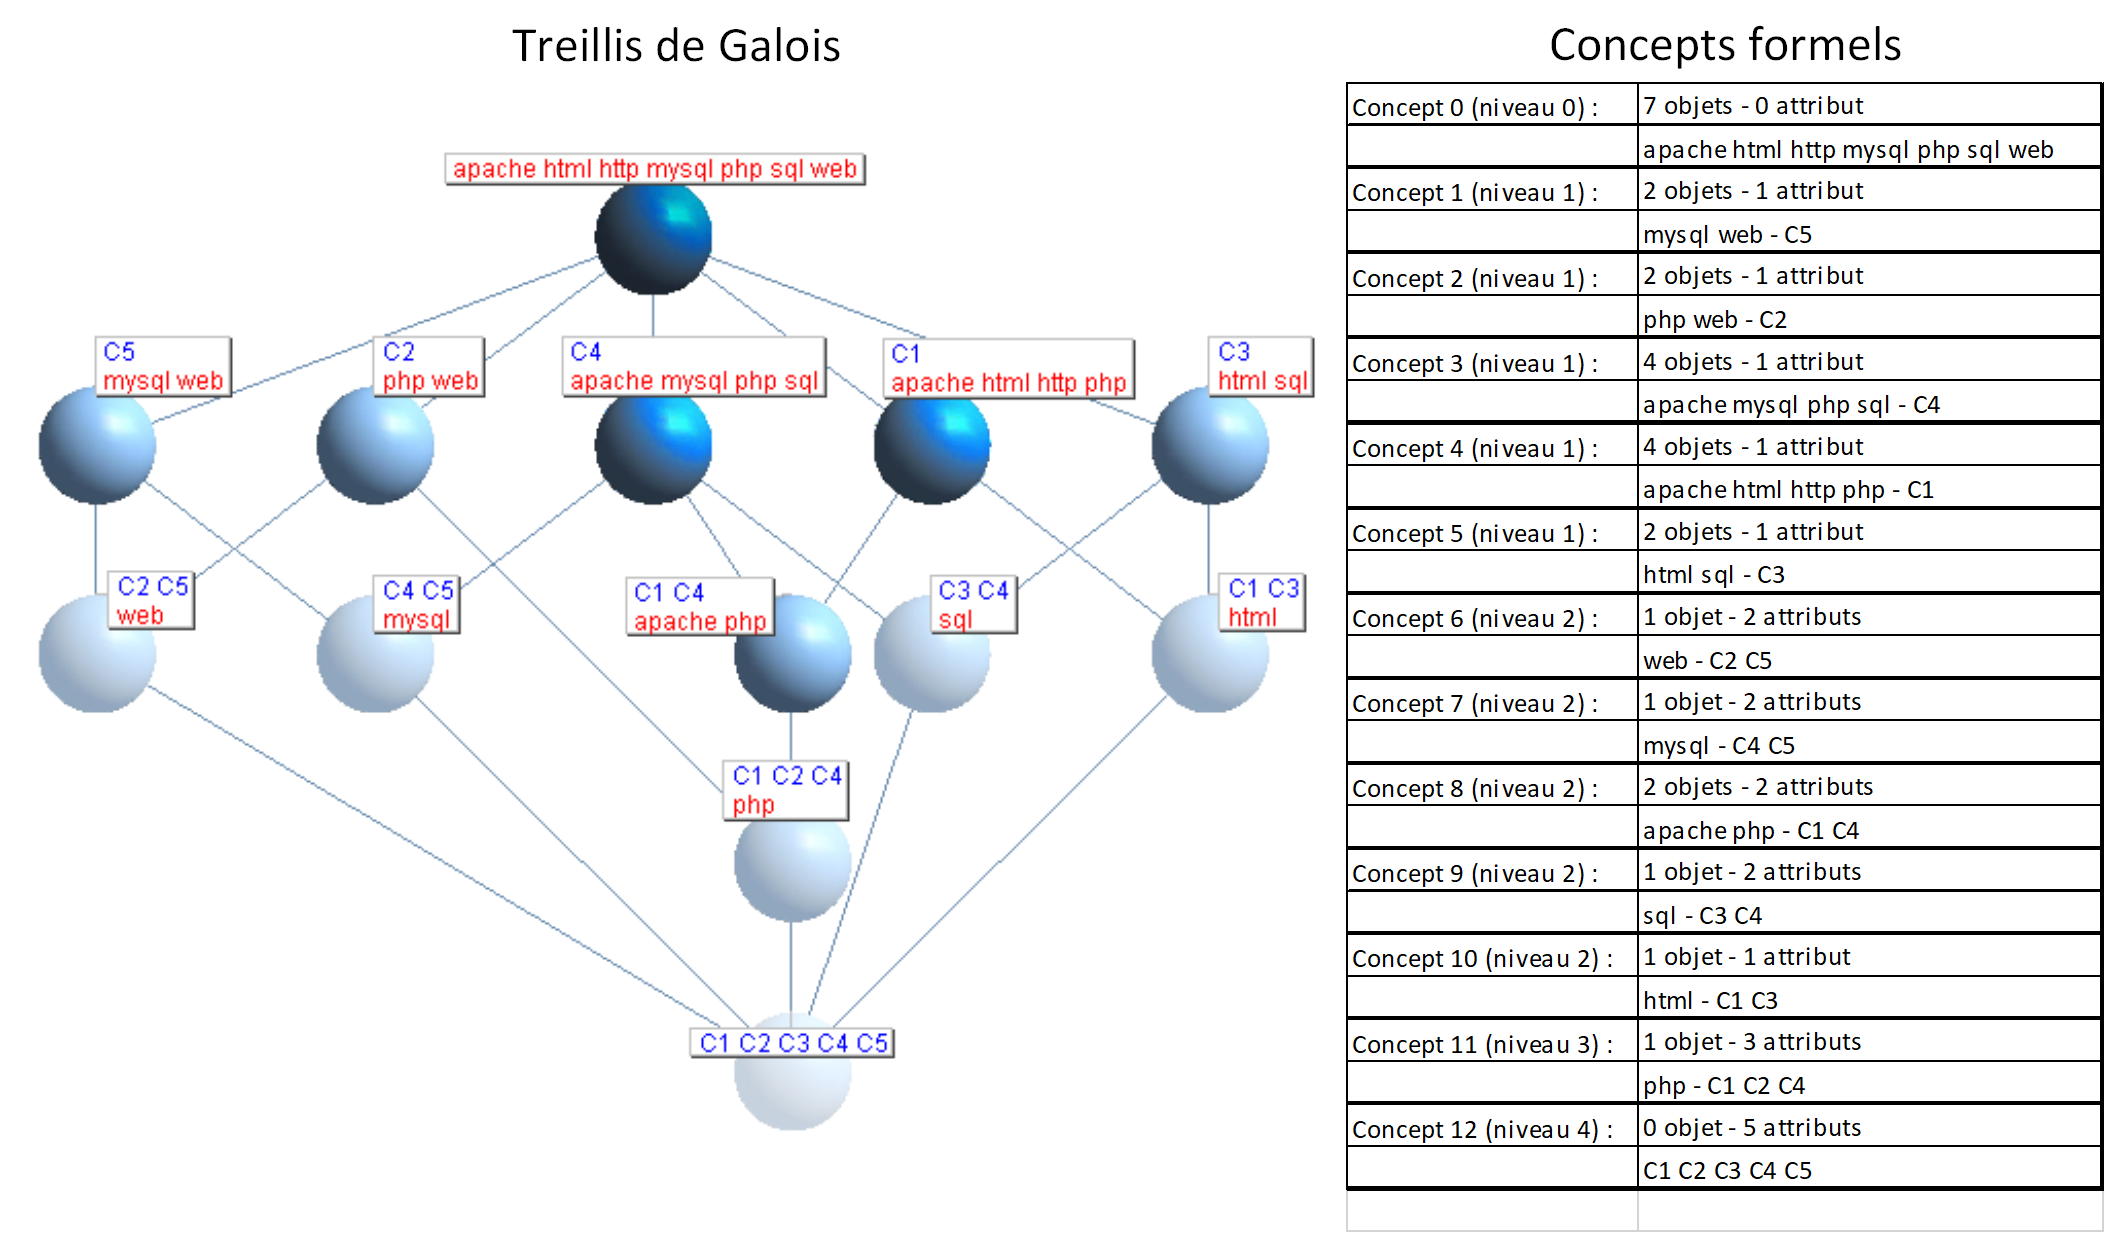
\includegraphics[scale=0.7]{2-Etat-de-l'Art/images/ACF/Treillis/exemple_treillis-concepts_ExampleMediumMatrix-S-B-B-0.00.png}
}
\caption{Treillis de Galois et ses concepts formels}
\label{figure:2-S2-Treillis-Concepts}
\end{figure}
%\end{figure*} % Figure flottante
% To use it : fig~\ref{label}

\bigskip

Dans l'exemple précédent, treize concepts formels ont été générés à partir du contexte formel pour construire le treillis de Galois (ceux-ci sont explicités sur la figure~\ref{figure:2-S2-Treillis-Concepts}).
Ces concepts formels regroupent donc des termes et les documents auxquels ils sont rattachés, c'est-à-dire, suite aux stratégies de binarisation, chaque concept formel rassemble des termes qui apparaissent ensemble dans un ou plusieurs documents selon leurs fréquences d'apparitions communes.
Les concepts formels ainsi formés permettent de manipuler des informations plus abstraites grâce à la combinaison de termes et documents engendrée par le treillis de Galois.


%\bigskip
\newpage % esthétique

%%%%%%%%%%%%%%%%%%%%%%%%%%%%%%%%%%%%%%%%%%%%
%\clearpage % Clean for pictures and tables %
%\newpage   % Clean for pictures and tables %
%%%%%%%%%%%%%%%%%%%%%%%%%%%%%%%%%%%%%%%%%%%%

\subsubsection{Calcul des métriques du treillis (PII.1.e) :}
\label{subsubsection:Contexte:ACF-MetriquesTreillis}

L'ACF permet de calculer de nombreuses métriques sur le treillis généré~\cite{babin2012approximating}\cite{jaffal2019aide} : stabilité des concepts, poids conceptuel des objets (respectivement des attributs), similarité conceptuelle des objets (respectivement des attributs), impact mutuel absolu entre un objet et un attribut, impact mutuel relatif entre un objet et un attribut, et beaucoup d'autres.
Dans le cas de la méthode CREA, nous nous concentrons particulièrement sur l'impact mutuel relatif~\cite{jaffal2019aide} qui permet de générer des graphiques utiles pour évaluer la qualité des données (présentés en sous-section~\ref{subsection:CREA:PII.2-GrapheImpactMutuel}), ainsi que la similarité conceptuelle des objets~\cite{jaffal2019aide} nécessaire pour d'autres traitements ultérieurs (notamment lors du regroupement des termes présenté en sous-section~\ref{subsection:CREA:PII.3-ConstructionClusters}).

\bigskip

\paragraph{Similarité Conceptuelle entre deux objets :}
\label{mystep:Contexte:ACF-MetriquesTreillis-SimilariteConceptuelle}

La \textit{similarité conceptuelle} permet de comparer deux objets (respectivement attributs) en tenant compte de leurs présences dans l'ensemble du treillis.
C'est-à-dire, la métrique correspond à la fréquence d'apparition des objets dans les concepts formels du treillis.
La formule calculant la similarité conceptuelle entre deux objets est la suivante :

\begin{equation}
\text{\textit{Similarité conceptuelle}}(O_{i}, O_{j}) = \frac{\text{\textit{Nombre de concepts contenant} } O_{i} \text{ \textbf{et} } O_{j}}{\text{\textit{Nombre de concepts contenant} } O_{i} \text{ \textbf{ou} } O_{j}}
\label{equation:2-S2-Metriques-SimilariteConceptuelle}
\end{equation}

La similarité conceptuelle étant un rapport, elle prend des valeurs entre $ 0 $ et $ 1 $.
La valeur maximale $ 1 $ indique que les deux objets (respectivement attributs) sont toujours présents ensemble dans les mêmes concepts formels du treillis, c'est-à-dire qu'il n'existe aucun concept formel ne contenant que l'un des deux objets (respectivement attributs), ou encore qu'ils partagent exactement les mêmes attributs (respectivement objets).
L'exemple en figure~\ref{figure:2-S2-Metriques-SimilariteConceptuelle-Exemple} illustre le calcul de la similarité entre deux objets.

\bigskip

Il est possible de générer un tableau regroupant les similarités conceptuelles entre tous les objets (respectivement attributs) d'un treillis, ce qui a pour conséquence de former une \textit{matrice de similarité conceptuelle}.
La figure~\ref{figure:2-S2-Metriques-SimilariteConceptuelle-Matrice} illustre une matrice de similarité conceptuelle regroupant les similarités conceptuelles de tous les objets d'un treillis.

\bigskip

Dans le cadre de la méthode CREA, la matrice de similarité conceptuelle est une donnée d'entrée aux méthodes de \textit{clustering} abordées plus tard en sous-section~\ref{subsection:CREA:PII.3-ConstructionClusters}.

\bigskip

\vfill
\hspace{0pt}

%%%%%%%%%%%%%
%% ESTHETIQUE

\begin{figure}[htb!]
\centering
\centerline{  % FORCE FIGURE OUTSIDE THE MARGIN !!! BUT STILL CENTERING !!!
% scale = 0.85
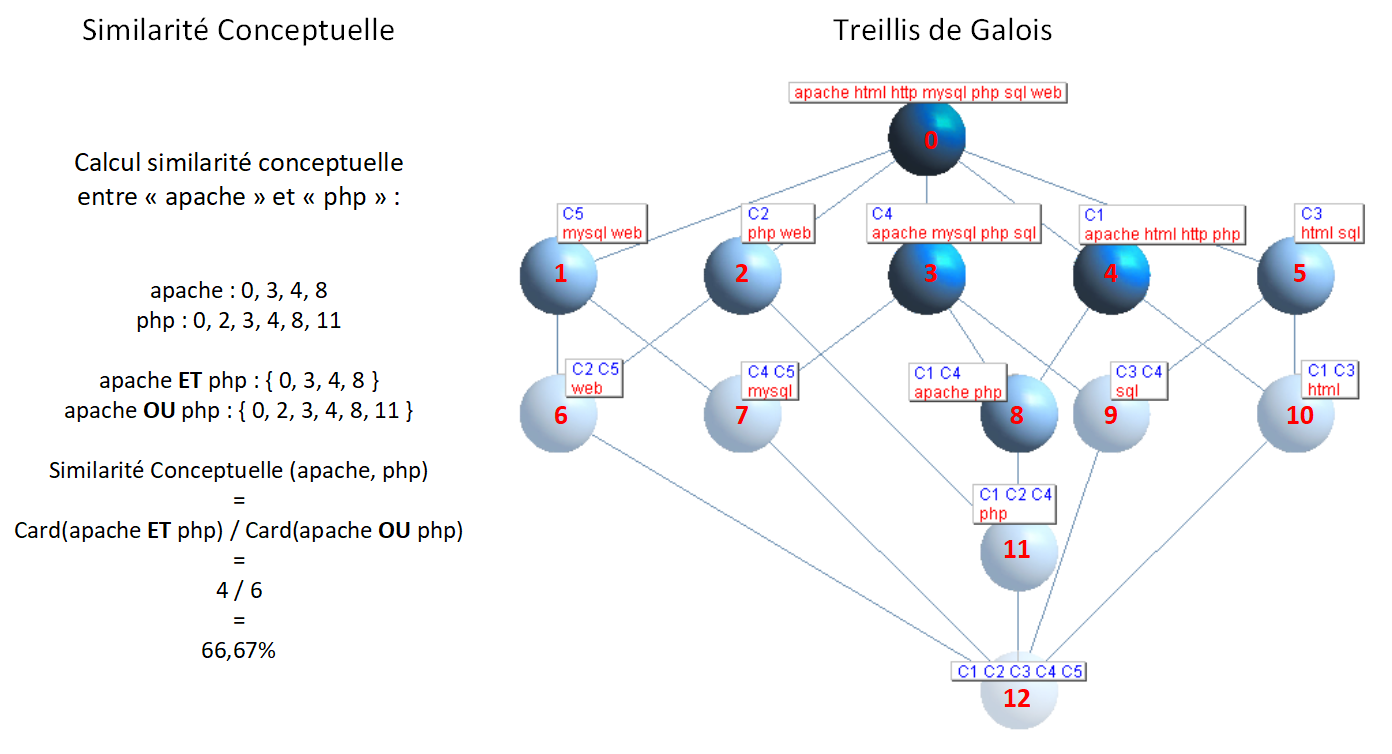
\includegraphics[scale=1]{2-Etat-de-l'Art/images/ACF/Metriques/exemple_similarite-conceptuelle_calcul.png}
}
\caption{Calcul de la similarité conceptuelle entre deux objets}
\label{figure:2-S2-Metriques-SimilariteConceptuelle-Exemple}
\end{figure}

\hspace{0pt}
\vfill

\newpage % esthétique

\begin{figure}[htb!]
\centering
%\includegraphics[width=3in]{images/VerySmallModels_text.png}
%%\includegraphics[scale=0.6]{images/VerySmallModels_text.png}
\centerline{  % FORCE FIGURE OUTSIDE THE MARGIN !!! BUT STILL CENTERING !!!
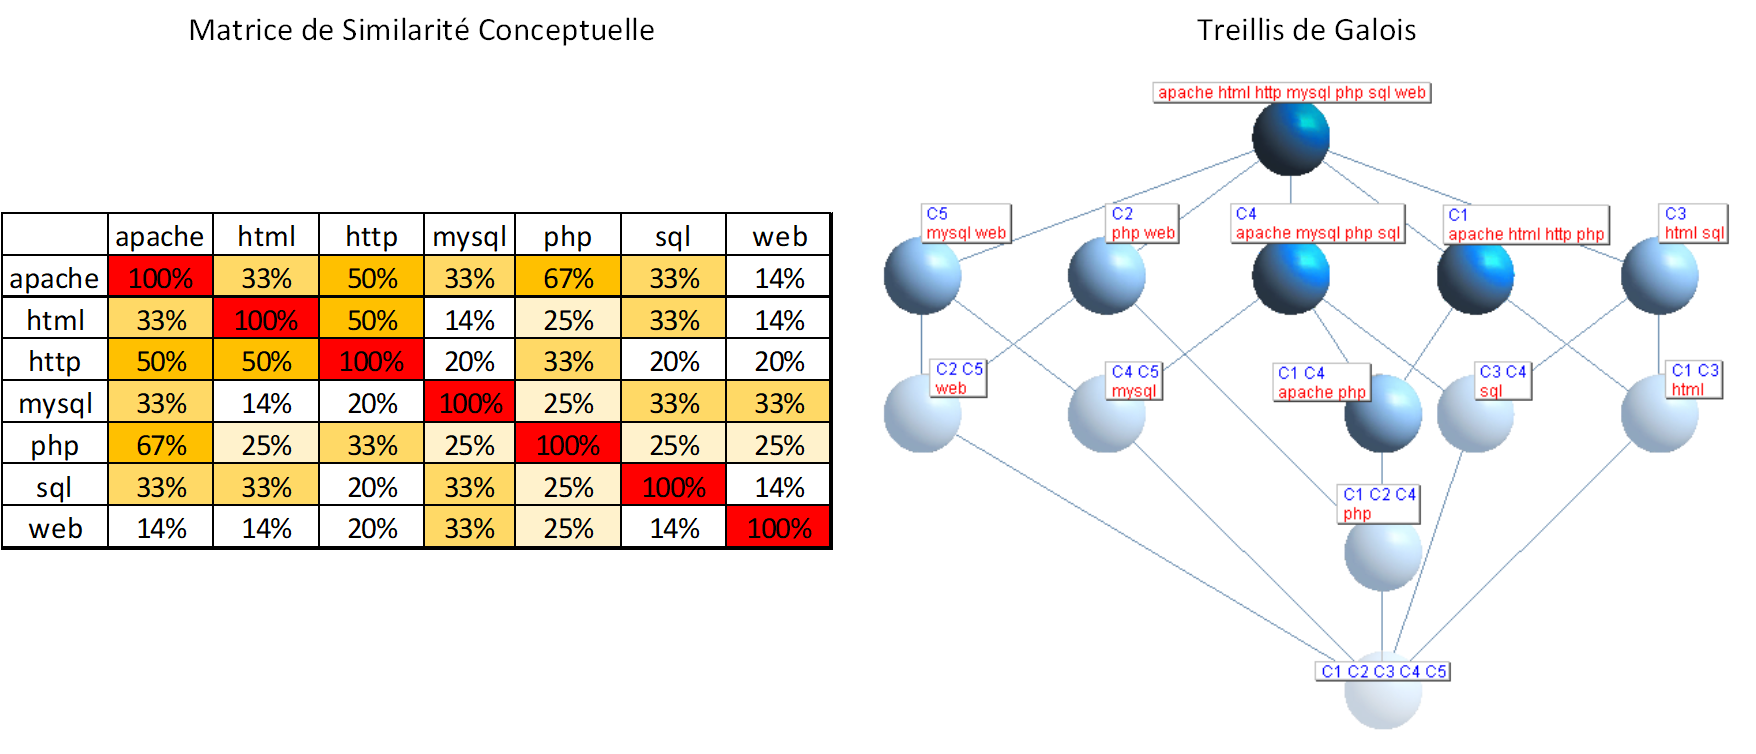
\includegraphics[scale=0.85]{2-Etat-de-l'Art/images/ACF/Metriques/exemple_similarite-conceptuelle_matrice.png}
}
\caption{Matrice de similarité conceptuelle}
\label{figure:2-S2-Metriques-SimilariteConceptuelle-Matrice}
\end{figure}

%% FIN ESTHETIQUE
%%%%%%%%%%%%%

\bigskip

%\clearpage % Clean for pictures and tables %


\paragraph{Impact mutuel entre un objet et un attribut :}
\label{mystep:Contexte:ACF-MetriquesTreillis-ImpactMutuel}

L'\textit{impact mutuel} analyse la "\textit{force de la relation entre un objet O$_{i}$ et un attribut A$_{j}$ en fonction des concepts formels qui les associent}"~\cite{jaffal2019aide}.
Il est défini à partir de l'équation suivante :

\bigskip

\begin{equation}
\text{\textit{Impact mutuel}}(O_{i}, A_{j}) = \frac{\text{\textit{Nombre de concepts contenant} } O_{i} \text{ \textbf{et} } A_{j}}{\text{\textit{Nombre de concepts contenant} } O_{i} \text{ \textbf{ou} } A_{j}}
\label{equation:2-S2-Metriques-ImpactMutuel}
\end{equation}


\bigskip % esthétique

L'impact mutuel étant un rapport, il prend des valeurs entre $ 0 $ et $ 1 $.
Plus la valeur de l'impact mutuel est élevée, plus l'attribut caractérise l'objet parmi tous les autres, et réciproquement : plus l'objet se définit particulièrement grâce à cet attribut.
En d'autres termes, un impact mutuel proche de $ 1 $ implique que l'attribut apparait quasiment uniquement avec cet objet, et réciproquement, l'objet n'a quasiment pas d'autre attribut.
À l'inverse, un impact mutuel proche de $ 0 $, mais non nul, implique que l'attribut est partagé par énormément d'objets, et réciproquement, que l'objet utilise quasiment tous les attributs existants.
L'exemple en figure~\ref{figure:2-S2-Metriques-ImpactMutuel-Exemple} illustre le calcul de l'impact mutuel entre un objet et un attribut.

%\begin{figure*} % Figure flottante
\begin{figure}[htb!]
\centering
%\includegraphics[width=3in]{images/VerySmallModels_text.png}
%%\includegraphics[scale=0.6]{images/VerySmallModels_text.png}
\centerline{  % FORCE FIGURE OUTSIDE THE MARGIN !!! BUT STILL CENTERING !!!
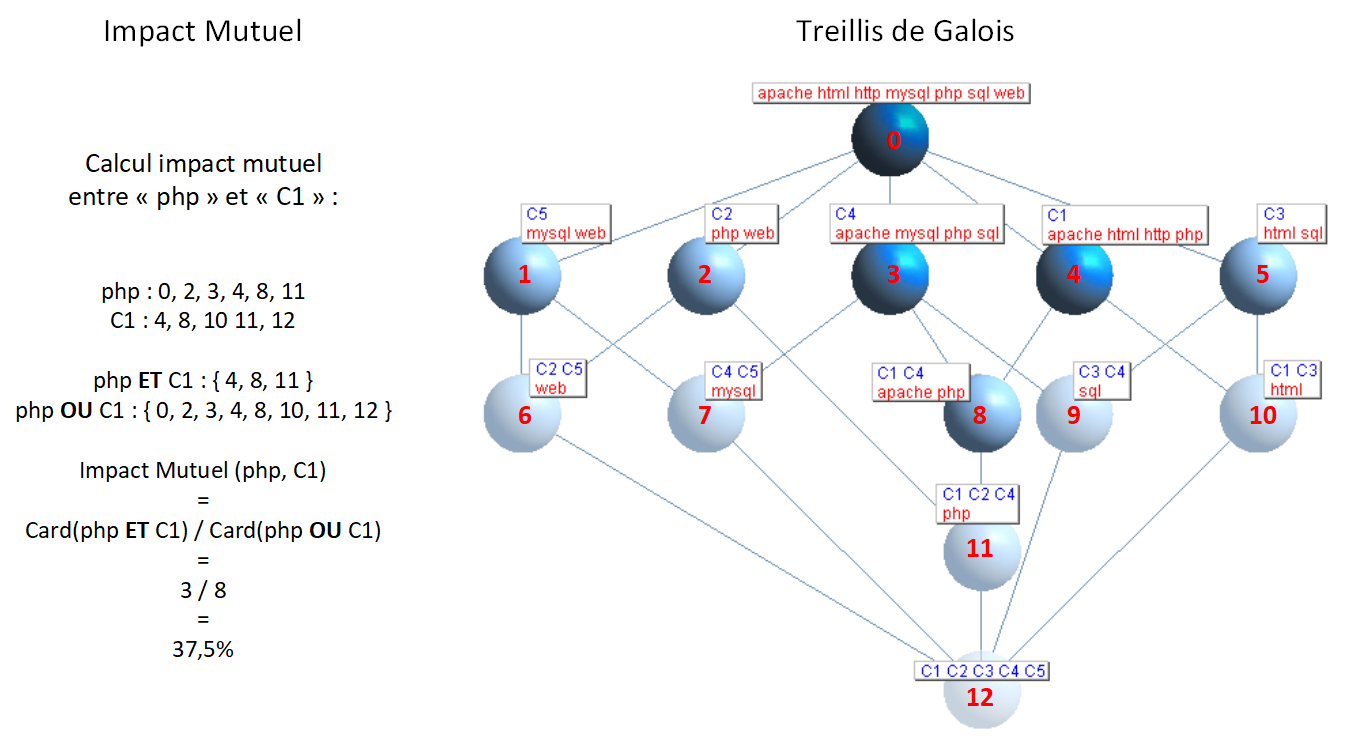
\includegraphics[scale=1]{2-Etat-de-l'Art/images/ACF/Metriques/exemple_impact-mutuel_calcul.png}
}
\caption{Calcul de l'impact mutuel entre un objet et un attribut}
\label{figure:2-S2-Metriques-ImpactMutuel-Exemple}
\end{figure}
%\end{figure*} % Figure flottante
% To use it : fig~\ref{label}

Le tableau regroupant les impacts mutuels entre tous les objets et attributs d'un treillis s'appelle une \textit{matrice d'impact mutuel}.
La figure~\ref{figure:2-S2-Metriques-ImpactMutuel-Matrice} illustre une matrice d'impact mutuel regroupant les impacts mutuels entre chaque objet et chaque attribut d'un treillis.

%\begin{figure*} % Figure flottante
\begin{figure}[htb!]
\centering
\centerline{  % FORCE FIGURE OUTSIDE THE MARGIN !!! BUT STILL CENTERING !!!
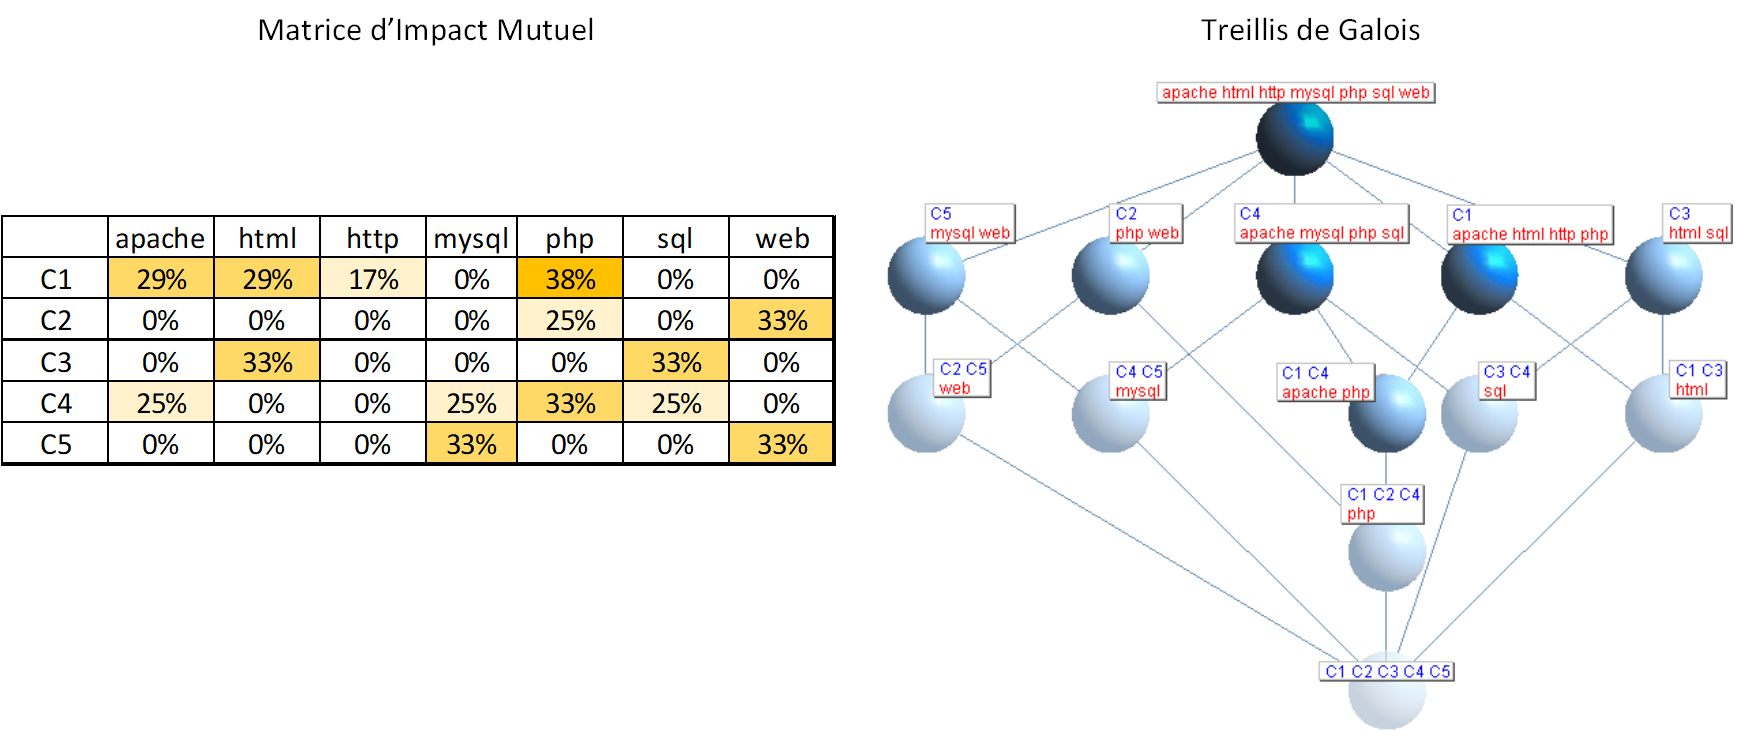
\includegraphics[scale=0.8]{2-Etat-de-l'Art/images/ACF/Metriques/exemple_impact-mutuel_matrice.png}
}
\caption{Matrice d'impact mutuel}
\label{figure:2-S2-Metriques-ImpactMutuel-Matrice}
\end{figure}
%\end{figure*} % Figure flottante
% To use it : fig~\ref{label}

\bigskip

La matrice d'impact mutuel permet de générer un \textit{graphe d'impact mutuel}.
Le graphe d'impact mutuel a la particularité d'être bi-parti, en proposant des n\oe{}uds de la classe des objets, et des n\oe{}uds de la classe des attributs.
Dans le cadre de la méthode CREA, ce graphe permet de déterminer visuellement deux informations importantes : les termes les plus représentatifs du corpus de documents rassemblés ; la pertinence des documents dans le contexte ainsi formé.
La figure~\ref{figure:2-S2-Metriques-ImpactMutuel-Graphe} illustre le graphe d'impact mutuel et fait un agrandissement de l'ensemble central où le document \textit{C1} apparait parmi des termes.

%\begin{figure*} % Figure flottante
\begin{figure}[htb!]
\centering
\centerline{  % FORCE FIGURE OUTSIDE THE MARGIN !!! BUT STILL CENTERING !!!
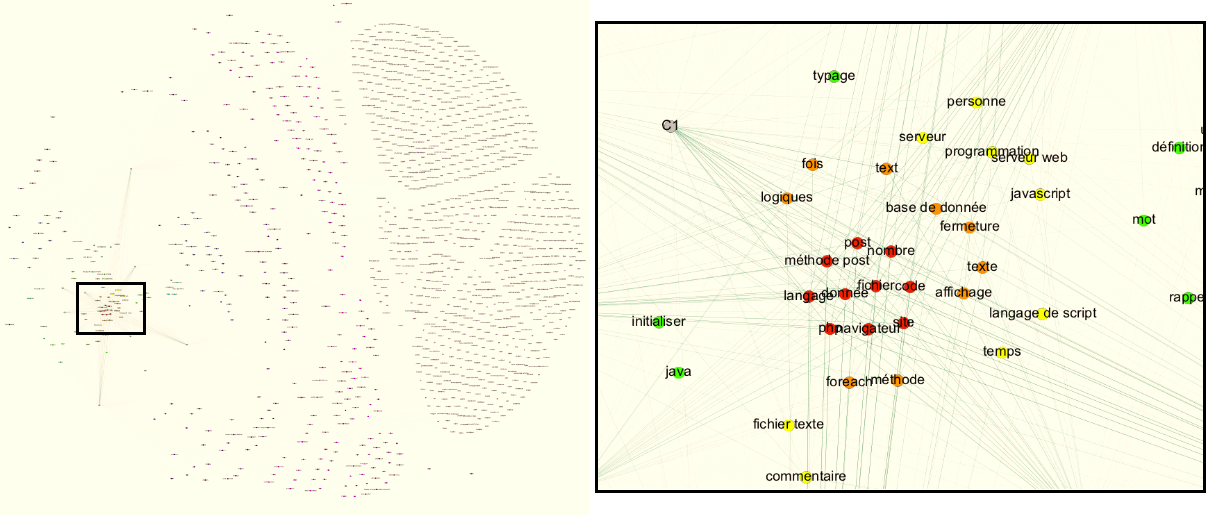
\includegraphics[scale=0.6]{2-Etat-de-l'Art/images/ACF/Metriques/exemple_graphe.png}
}
\caption{Graphe d'impact mutuel (généré avec Gephi en utilisant la spatialisation \textit{Force Atlas} et la coloration par \textit{partition} selon le \textit{degré}) et agrandissement de la communauté centrale}
\label{figure:2-S2-Metriques-ImpactMutuel-Graphe}
\end{figure}
%\end{figure*} % Figure flottante
% To use it : fig~\ref{label}

\bigskip

Typiquement, un ou des documents excentrés et avec peu de liens peuvent être considérés comme peu pertinents, voire comme du \textit{bruit} d'un point de vue statistique.
Ces documents peu pertinents peuvent être supprimés de la matrice d'occurrences (voir les sous-section~\ref{subsubsection:CREA:PII.1.a-normalisation} et~\ref{subsection:CREA:PII.2-GrapheImpactMutuel}) pour améliorer la qualité des résultats, ou peuvent être conservés si l'utilisateur l'exige.
La même réflexion peut être appliquée sur un ou des termes trop isolés (avec peu de liens).
Une fois supprimés de la matrice d'occurrences, il suffit de relancer les traitements depuis l'étape \textit{normalisation} (voir la sous-section~\ref{subsubsection:CREA:PII.1.a-normalisation}).
Cependant, si l'utilisateur estime que ces documents ou termes sont nécessaires, ceux-ci peuvent être conservés.

\bigskip

L'impact mutuel, et sa représentation graphique, mettent en évidence certaines qualités des documents et termes : un utilisateur comprend visuellement quels documents et termes sont importants du point de vue de l'ensemble des cas passés, mais surtout lesquels sont considérés comme peu importants ou peu pertinents.
Il faut rappeler que les résultats de cette métrique dépendent directement de deux paramètres (les cas passés dont les documents ont été sélectionnés et donnés en entrée de la méthode, et le choix de la stratégie de binarisation) et indirectement de deux paramètres (la technique de TAL employée et sa base de connaissances).
La faible représentativité d'un terme ou d'un document peut s'expliquer de plusieurs façons, mais il est important que l'utilisateur choisisse de conserver ou supprimer les termes et documents selon le cas qu'il cherche à construire.



\bigskip

Pour conclure cette sous-section, il est important de noter que d'autres travaux de thèse~\cite{tang2016interactive} ont développé et éprouvé une approche similaire à celle présentée dans cette thèse.
\textit{KESAM (Knowledge Extraction and Semantic Annotation Management)} est un outil basé sur l'usage d'annotation sémantique depuis une base de connaissances et d'ACF pour aider des experts à analyser des documents et leurs contenus textuels.
Cependant, ces travaux se limitent à présenter et manipuler le treillis construit, son contexte formel, et les liens avec les documents d'origine.
Dans les travaux présentés dans cette thèse, nous utilisons en complément deux des métriques présentées dans~\cite{jaffal2019aide} afin d'interpréter les données issues du treillis, pour non seulement détecter la pertinence des supports de cours en entrée, mais surtout pour générer des clusters de notions réutilisables.




\bigskip

%%%%%%%%%%%%%%%%%%%%%%%%%%%%%%%%%%%%%%%%%%%%
%\clearpage % Clean for pictures and tables %
%\newpage   % Clean for pictures and tables %
%%%%%%%%%%%%%%%%%%%%%%%%%%%%%%%%%%%%%%%%%%%%


\subsection{Clustering}
\label{subsection:Contexte:TechniquesUtilisees:Clustering}

Dans le domaine de la fouille de données, plusieurs activités visent à regrouper et classifier les données dans des catégories (ou classes) selon des propriétés communes ou des critères de similarité~\cite{xu2008clustering}.
Deux familles de méthodes cohabitent : les méthodes d'apprentissage supervisé (plutôt pour classifier), et les méthodes d'apprentissage non-supervisé (plutôt pour du clustering)~\cite{rokach2005clustering}.
L'apprentissage supervisé vise à entrainer un modèle à reconnaitre des catégories existantes (connues grâce à des données étiquetées) afin d'y classer les données d'entrée~\cite{xu2008clustering}, ou éventuellement de découvrir de nouvelles catégories~\cite{jain1999data}.
L'apprentissage non-supervisé vise à séparer les données dans un certain nombre de groupes selon des critères peu évidents, voire dans des structures cachées~\cite{xu2008clustering}.
\og \textit{Le but du clustering est descriptif, là où la classification est prédictive} \fg~\cite{rokach2005clustering}\cite{veyssieres1998identification} (\og \textit{The goal of clustering is descriptive, that of classification is predictive} \fg).

\bigskip

Appliquées à nos travaux pour extraire des fragments réutilisables, en particulier pour la recherche de patterns, les méthodes de clustering sont fortement adaptées~\cite{jain1999data}.
Le clustering contient néanmoins des méthodes impliquant un entraînement préalable, mais nous ne les aborderons pas.
Nous nous intéressons en particulier aux méthodes ne nécessitant aucun entraînement, afin de les laisser rechercher les similarités sans à priori.
Il est difficile de définir la notion de \textit{cluster}~\cite{estivill2000fast}\cite{everitt2011cluster}, nous nous contenterons donc de considérer qu'il s'agit d'un regroupement d'objets selon des caractéristiques communes, donc de cohésion interne/homogénéité et d'isolation externe comme décrit par~\cite{cormack1971review} et~\cite{gordon1999classification}.

\bigskip

D'après~\cite{fraley1998many}, on peut diviser les méthodes de clustering en deux grandes familles dont les \textit{méthodes de partitionnement} et les \textit{méthodes hiérarchiques} (d'autres façons d'organiser sont présentées dans~\cite{rokach2005clustering}).
Ces deux familles sont décrites ainsi dans~\cite{rokach2005clustering} :

\begin{itemize}
\item Les méthodes de partitionnement placent tout d'abord les données d'entrée dans un ou plusieurs clusters, puis déplacent les données d'un cluster à l'autre afin d'obtenir un placement optimal.
Généralement, l'utilisateur doit indiquer le nombre de clusters désirés.
On peut citer parmi ces algorithmes : \textit{K-Means}, \textit{K-medoids}, \textit{DBSCAN}, \textit{OPTICS}, \textit{Minimal Spanning Tree}, ...\\

\item Les méthodes hiérarchiques construisent progressivement les clusters, soit en divisant l'ensemble des données, soit en les agrégeant au fur et à mesure (les modifications deviennent définitives : un objet manipulé ne peut plus se déplacer).
Ces méthodes reposent elles-mêmes sur deux principes : un fonctionnement ascendant (chaque objet démarre dans son propre cluster, chaque itération regroupe deux clusters selon une métrique de distance jusqu'à n'en obtenir qu'un seul), un fonctionnement descendant (tous les objets démarrent dans le même cluster, chaque itération sépare un cluster en deux).
Ces méthodes proposent une représentation graphique appelée \textit{dendrogramme}.
La \textit{classification ascendante hiérarchique} (CAH), ou \textit{hierarchical cluster analysis} (HCA) en anglais, est la principale méthode employée.
\end{itemize}

\bigskip

Certains algorithmes de clustering peuvent générer des classes recouvrantes (ou chevauchantes), c'est-à-dire qu'un même objet se retrouve simultanément dans plusieurs classes.
Parmi ces techniques se trouve par exemple la \textit{Classification Ascendante Pyramidale} et les pyramides~\cite{diday1984representation} se rapprochant de la CAH et des dendrogrammes, ou encore OKM~\cite{cleuziou2008extended} (\textit{Overlapping K-Means}) une extension de K-Means.

\bigskip

Dans le cadre de nos travaux, afin de créer des fragments réutilisables issus de cas passés, nous visons la construction de clusters (l'équivalent des fragments) à partir de termes extraits des documents (les données à proposer à l'utilisateur).
Les traitements de l'ACF permettent d'obtenir une matrice de similarité (voir sous-section~\ref{mystep:Contexte:ACF-MetriquesTreillis-SimilariteConceptuelle}) à partir de laquelle nous pouvons déduire une similarité entre les objets contenus.
Parmi les deux familles de méthodes de custering, certains algorithmes nécessitent un placement des points dans un espace (parfois en deux dimensions, parfois à N dimensions), d'autres uniquement les distances ou similarités entre les objets.
Afin d'exploiter au mieux les distances entre objets, tout en évitant une distorsion trop élevée par l'usage du \textit{multidimensional scaling}~\cite{kruskal1978multidimensional}\cite{young1983multidimensional} réduisant à deux dimensions nos données, nous avons préféré l'utilisation de la \textit{classification ascendante hiérarchique} (CAH).

\bigskip

\subsubsection{Classification Ascendante Hiérarchique}
\label{subsubsection:Contexte:TechniquesUtilisees:Clustering:CAH}

La \textit{classification ascendante hiérarchique} (CAH) est une méthode hiérarchique agglomérant un à un chaque objet aux autres.
Par définition, cette méthode est donc non-recouvrante (un objet ne peut être que dans un seul cluster à la fois).
À partir d'une matrice contenant les distances entre chaque objet, le fonctionnement général est le suivant~\cite{xu2008clustering} :

\begin{enumerate}
\item Mettre chaque objet dans son propre cluster
\item Calculer les distances entre les clusters (dépendant de la métrique choisie)
\item Fusionner les clusters les plus proches
\item S'il reste plus d'un cluster, répéter depuis l'opération 2
\item Sinon, découper les clusters au partir du niveau souhaité
\end{enumerate}

\bigskip

La figure~\ref{figure:2-S2-Exemple-CAH-Dendrogramme-2} illustre le dendrogramme construit à partir de la matrice de distance, puis la création des clusters lorsque ce dendrogramme est coupé à la hauteur $ 3 $.
L'axe des abscisses représente les distances entre les éléments (et clusters après fusion), et l'axe des ordonnées représente les éléments à regrouper en clusters.
Dans l'ensemble de la matrice de distance, les objets C et D sont les plus proches par rapport aux autres, ils sont donc fusionnés en premiers.
Ensuite, le recalcul de la matrice de distance fait que A se trouve être le plus proche du cluster contenant C et D, A est donc ajouté à ce cluster.
Finalement, le dernier élément B est ajouté au cluster.
Lorsque l'on découpe le dendrogramme à la hauteur $ 3 $ (la ligne rouge en pointillés), on obtient trois clusters.

\bigskip

Plusieurs métriques de distance existent afin de déterminer comment agréger ou découper les clusters.
Le \textit{saut minimum} (ou \textit{single linkage} en anglais) consiste à considérer la distance entre deux clusters comme étant la distance des deux objets les plus proches de chacun des clusters~\cite{saporta2006probabilites}.
À l'inverse, le \textit{complete linkage} en anglais, consiste à considérer la distance entre deux clusters comme étant la distance des deux objets les plus éloignés de chacun des clusters~\cite{saporta2006probabilites}.
D'autres métriques basées sur la moyenne des distances des points des clusters, ou encore sur les centroïdes des clusters permettent de déterminer les clusters les plus proches à fusionner.

\bigskip

%\begin{figure*} % Figure flottante
\begin{figure}[ht]
\centering
\centerline{  % FORCE FIGURE OUTSIDE THE MARGIN !!! BUT STILL CENTERING !!!
% scale = 0.7
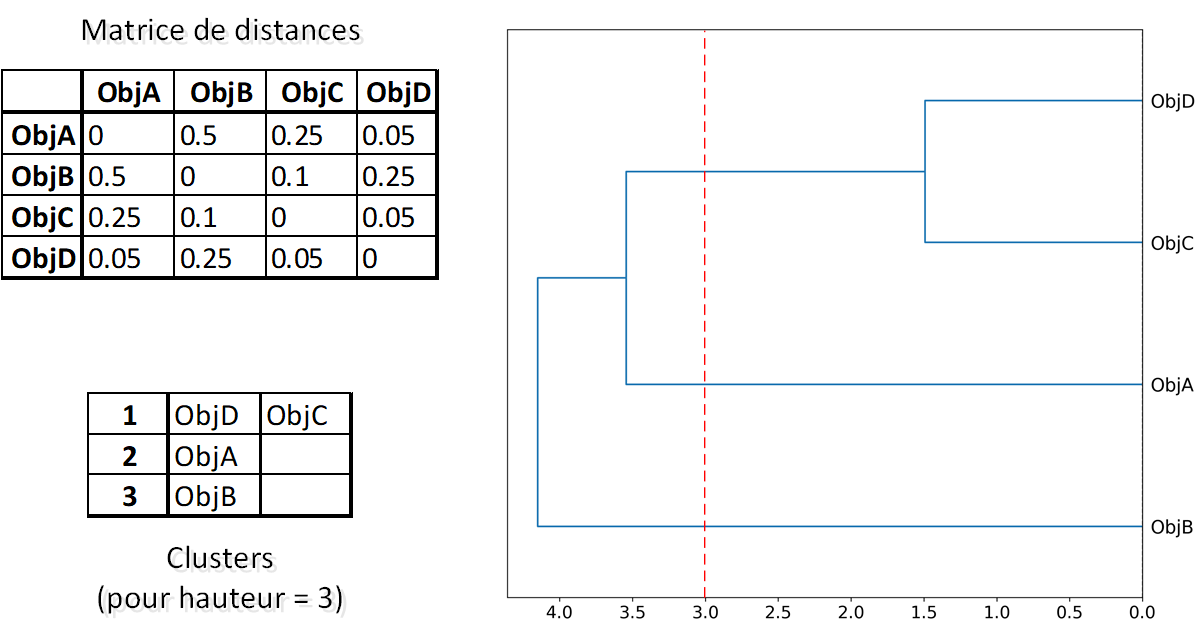
\includegraphics[scale=1]{2-Etat-de-l'Art/images/Clustering/CAH-exemple2.png}
}
\caption{Exemple de construction du dendrogramme et des clusters à la hauteur 3 à partir d'une matrice de distance}
\label{figure:2-S2-Exemple-CAH-Dendrogramme-2}
\end{figure}
%\end{figure*} % Figure flottante
% To use it : fig~\ref{label}





%%%%%%%%%%%%%%%%%%%%%%%%%%%%%%%%%%%%%%%%%%%%%%%%%%%%%%%%%%%%%%%%%%%%%%%%%%%%%%%%%%%%%%%%%%
%%%%%%%%%%%%%%%%%%%%%%%%%%%%%%%%%%%%%%%%%%%%%%%%%%%%%%%%%%%%%%%%%%%%%%%%%%%%%%%%%%%%%%%%%%
%%%%%%%%%%%%%%%%%%%%%%%%%%%%%%%%%%%%%%%%%%%%%%%%%%%%%%%%%%%%%%%%%%%%%%%%%%%%%%%%%%%%%%%%%%
%%%%%%%%%%%%%%%%%%%%%%%%%%%%%%%%%%%%%%%%%%%%%%%%%%%%%%%%%%%%%%%%%%%%%%%%%%%%%%%%%%%%%%%%%%
%%%%%%%%%%%%%%%%%%%%%%%%%%%%%%%%%%%%%%%%%%%%%%%%%%%%%%%%%%%%%%%%%%%%%%%%%%%%%%%%%%%%%%%%%%
%%%%%%%%%%%%%%%%%%%%%%%%%%%%%%%%%%%%%%%%%%%%%%%%%%%%%%%%%%%%%%%%%%%%%%%%%%%%%%%%%%%%%%%%%%

%%%%%%%%%%%%%%%%%%%%%%%%%%%%%%%%%%%%%%%%%%%%
\clearpage % Clean for pictures and tables %
\newpage   % Clean for pictures and tables %
%%%%%%%%%%%%%%%%%%%%%%%%%%%%%%%%%%%%%%%%%%%%

%%%%%%%%%%%%%%%%%%%%%%%%%%%%%%%%%%%%%%%%%%%%%%%%%%%%%%%%%%%%%%%%%%%%%%%%%%%%%%%%%%%%%%%%%%
%%%%%%%%%%%%%%%%%%%%%%%%%%%%%%%%%%%%%%%%%%%%%%%%%%%%%%%%%%%%%%%%%%%%%%%%%%%%%%%%%%%%%%%%%%
%%%%%%%%%%%%%%%%%%%%%%%%%%%%%%%%%%%%%%%%%%%%%%%%%%%%%%%%%%%%%%%%%%%%%%%%%%%%%%%%%%%%%%%%%%
%%%%%%%%%%%%%%%%%%%%%%%%%%%%%%%%%%%%%%%%%%%%%%%%%%%%%%%%%%%%%%%%%%%%%%%%%%%%%%%%%%%%%%%%%%
%%%%%%%%%%%%%%%%%%%%%%%%%%%%%%%%%%%%%%%%%%%%%%%%%%%%%%%%%%%%%%%%%%%%%%%%%%%%%%%%%%%%%%%%%%
%%%%%%%%%%%%%%%%%%%%%%%%%%%%%%%%%%%%%%%%%%%%%%%%%%%%%%%%%%%%%%%%%%%%%%%%%%%%%%%%%%%%%%%%%%


\section{Travaux connexes et similaires}
\label{section:Contexte:TravauxConnexes}

Afin de surmonter les défis rencontrés par les processus à forte intensité de connaissances, et contribuer à la réutilisation de fragments de processus et de leurs connaissances, plusieurs solutions ont été proposées dans la littérature.
Nous présentons maintenant ces solutions et leurs limites, puis nous positionnons notre propre solution.

\bigskip

\subsection{Travaux connexes sur les processus à forte intensité de connaissances}
\label{section:Contexte:TravauxConnexes:KIP}

La réutilisation et les fragments appliqués aux processus à forte intensité de connaissances se retrouvent dans plusieurs travaux.
L'usage de \textit{patterns}, c'est-à-dire des motifs qui se répètent, dans les outils BPM appliqués à des modèles de workflows (BPMN, EPC, ...) est connu et permet de proposer des ensembles de tâches et activités liées et prêtes à l'emploi.

Les travaux présentés dans~\cite{bider2018introducing} visent à expérimenter des patterns dans d'autres types de modèles, en particulier des patterns de buts appliqués au \textit{STate-oriented Business Process Modeling} (SToBPM), où les états sont représentés sous forme d'espace multidimensionnel.
Chaque dimension représente un paramètre, donc un point représente un résultat possible d'une instance de processus.
Si la dimension temporelle est ajoutée, une courbe permet de déterminer l'avancement du processus dans le temps.
Afin de représenter le processus et ses résultats de façon plus adaptée, des formulaires sont préférés en lieu et place de courbes dans des espaces multidimensionnels.
Les buts (et sous-buts) visés par le concepteur, permettant de choisir les patterns dans une bibliothèque, sont construits sur des \textit{décisions} (la finalité à atteindre), des \textit{problèmes} (auxquels appliquer les décisions), des \textit{motivations} (raisons pour lesquelles une décision a été prise, et/ou avancement du problème), des \textit{preneurs de décisions} (organisation, groupe, ou individu), et éventuellement une \textit{date limite} (gestion temporelle).
Un concepteur de processus choisit donc des patterns, s'il le souhaite, en indiquant les buts recherchés dans la bibliothèque.
Il dispose d'une grande liberté pour réutiliser ou non ces patterns, car l'utilisateur n'est pas guidé mais seulement assisté.

Ces travaux illustrent une autre façon de construire des patterns : au lieu de proposer des ensembles d'activités, le concepteur va rechercher des buts à atteindre et les activités nécessaires pour les valider.
La technique de modélisation est cependant beaucoup trop rigide pour être utilisée telle quelle pour des enseignements : bien qu'il soit nécessaire de s'inspirer de sources existantes, le nombre de dimensions finales est inconnu (tous comme le nombre d'états possibles), et les formulaires (ou le découpage en décisions, problèmes, motivations, preneurs de décisions, date limite) ne sont pas du tout adaptés à l'extraction de connaissances.

\bigskip

Dans~\cite{zasada2018box}, on trouve cette fois l'usage de \textit{compliance patterns}~\cite{elgammal2016formalizing} générés à partir de textes légaux pour permettre à des utilisateurs de construire et exécuter des processus respectant les réglementations en place.
La législation sur l'industrie alimentaire a été manuellement analysée afin de sélectionner plusieurs articles, les organiser en catégories et sous-catégories, et y retrouver des patterns fréquents.
Les exigences réglementaires ont ensuite été extraites et transformées en séquences de code, afin de pouvoir les préciser à l'aide des patterns.
Enfin, les patterns ont été formalisés sous forme de formules de \textit{logique linéaire temporelle} (ou \textit{linear temporal logic}/LTL en anglais).

Bien que la méthode puisse être appliquée à d'autres domaines, celle-ci n'est pas encore totalement supportée par les outils informatiques et nécessite plusieurs opérations manuelles.
De plus, il s'agit de patterns construits à partir de textes de loi en langage naturel, donc d'exigences à respecter.
Les supports de cours ayant comme objectif de transmettre des connaissances explicites, ceux-ci n'ont pas vocation à contraindre la conception ou l'exécution d'un processus.
On pourrait tout de même imaginer construire des patterns indiquant dans quel ordre aborder quelles notions lors d'un cours, mais cela implique de s'appuyer sur des textes explicitant ces informations sous forme d'assertions claires et non pas d'un enchaînement de notions comme dans les supports de cours classiques.

\bigskip

Parmi les approches CBR, les travaux présentés dans~\cite{cognini2016case} proposent un langage de modélisation de fragments de processus qui vise à générer et perfectionner manuellement des cas.
Ce langage, nommé \textit{Business Process Feature Model} (BPFM), permet de représenter les cas et leur contenu de façon plus complète que d'autres langages.
Plus spécifiquement, le BPFM est un langage déclaratif capable de représenter des processus partiellement structurés et ordonnés grâce à des contraintes, ainsi que des types de données complexes.
Le point le plus intéressant est sa capacité à représenter des variations de processus.
Les processus sont représentés sous forme d'arbres dont les n\oe{}uds correspondent aux sous-processus, et les feuilles aux activités atomiques.
Les contraintes permettent de déterminer si les activités et sous-processus peuvent ou doivent être utilisés dans les variants du processus, et s'ils peuvent ou doivent être exécutés dans ces variants.
BPFM permet également d'indiquer si des variations apparaissent lors de l'exécution du processus, et de retenir les liens de parentés entre les variations et les modèles initiaux.
Afin de conserver les connaissances liées au processus, l'\textit{Ontology-Based Case-Based Reasoning}~\cite{martin2013integrating} (OBCBR) est utilisée pour conserver les éléments décrivant l'objectif de chaque activité, les rôles de chaque intervenant, et l'auteur de la description du cas.
La réutilisation d'instances passées s'effectue de deux manières : lors de la phase de conception en indiquant les éventuelles variations, lors de l'exécution en modifiant selon les besoins chaque activité ou sous-processus.

Bien que ce langage offre une plus grande liberté d'exécution grâce aux contraintes et aux variations lors de l'exécution, les cas représentés restent fortement orientés du côté des processus métiers structurés : on représente un processus par un arbre de sous-processus et d'activités qui s'enchaînent.
Dans le cadre de la construction d'un cours, le syllabus pourrait être représenté sous forme d'arbre où les chapitres et sections formeraient différents niveaux, cependant, les connaissances que l'on cherche à transmettre ne sont pas de simples activités qu'il suffit de mentionner pour pouvoir les valider.
La réutilisation de cours passés implique d'assister à chaque cours ou de lire intégralement le contenu pour le modéliser, puis l'intégrer au modèle BPFM.
La difficulté réside dans l'association de certaines notions les unes avec les autres : il n'est pas possible en l'état de découvrir facilement les contraintes dans l'ordre des notions entre chaque variation de cours, car il s'agit de connaissances implicites à chaque enseignant.

\bigskip

Afin de mieux renseigner les gabarits réutilisables, les travaux dans~\cite{tenschert2016supporting} explorent l'usage de l'\textit{Acte de Langage} (ou \textit{Speech Act Theory} en anglais).
L'excès de gabarits, et le manque d'informations ou leur trop courte description pour les discerner clairement les uns des autres, implique que l'utilisateur doit rechercher lui-même l'objectif de chaque gabarit pour sélectionner le plus adapté à son cas.
Afin de retrouver plus rapidement le gabarit le plus adapté, les interactions et micro-processus sont analysés.
Un micro-processus est composé d'actes de coordination (équivalent de méta-données décrivant ce que le micro-processus vise à faire, qui l'exécute, envers quelle(s) autre(s) personne(s), le support, l'horodatage, le contenu, et d'autres annotations) et d'actes de production (création d'un artefact).
Les micro-processus s'appuient sur les actes de langage pour décrire toutes les informations des actes de coordination.
L'intérêt des micro-processus repose sur la possibilité laissée aux utilisateurs du métier de créer leurs propres gabarits selon les interactions qu'ils utilisent le plus souvent sans être perdus parmi d'immenses bibliothèques de gabarits.
Les connaissances tacites sont ainsi plus facilement mises à contribution dans les nombreuses méta-données des actes de coordination : les utilisateurs du métier emploient leur vocabulaire et modélisent leurs activités depuis leur propre point de vue, ils sont ainsi plus facilement capables de retrouver et réutiliser leurs propres gabarits.

Bien que ces travaux n'embarquent pour le moment qu'un petit sous-ensemble d'objets par rapport à ce que la gestion de cas préconise (documents, contacts, communications, ...), laisser les utilisateurs créer eux-mêmes des gabarits réutilisables à partir de leurs propres connaissances simplifie l'usage de la solution présentée.
Une limitation soulevée en conclusion dans~\cite{tenschert2016towards} indique que cette solution ne peut fonctionner que si les utilisateurs acceptent de renseigner chacun des micro-processus qu'ils utilisent.
Dans le cas de la construction de cours, on retrouve une limitation très proche : pour pouvoir réutiliser les supports de cours d'autres enseignants, il faut que tous les enseignants utilisent le même outil pour y insérer leurs connaissances.
Bien que PowerPoint et ses équivalents libres soient très fréquents, ceux-ci sont très rarement utilisés avec l'ensemble des fonctionnalités qui se rapprochent de la contribution décrite dans~\cite{tenschert2016supporting} (par exemple, les schémas sont souvent de simples images importées, et les méta-données des objets PowerPoint ne sont quasiment jamais renseignées).
Cependant, le vocabulaire du domaine et certaines activités (tels que les travaux dirigés ou pratiques) sont présents dans les diapositives qui peuvent être réutilisées à postériori par d'autres enseignants.

\bigskip

Du point de vue de la gestion des connaissances appliquée à la gestion de projets, une solution sur la réutilisation des connaissances est proposée dans~\cite{schacht2016methodology}.
Celle-ci se compose de trois parties :

\begin{itemize}
\item Un double-cycle dont la boucle choisie dépend du contexte de l'organisation et de l'équipe.
Récapitulatif : à la fin de chaque projet, l'équipe se réunit pour transférer son expérience aux autres équipes.
Préparation : au démarrage du projet ou d'une étape importante (c'est-à-dire \textit{pendant} le projet), l'équipe se réunit pour réfléchir à la conception de la solution à partir de l'expérience de chaque membre.

\item De nouveaux rôles sont définis pour retenir et transférer les expériences des équipes.
L'expert en leçons (\textit{lessons learned expert} en anglais) qui dispose de compétences pour traiter les connaissances et expériences issues de la réalisation du projet.
L'expert du sujet (\textit{topic expert} en anglais) qui dispose de connaissances et d'expérience sur le sujet traité par le projet.

\item Un processus centré sur les connaissances appliqué à la gestion de projet (\textit{knowledge-centric project management process} en anglais) s'appuyant sur le PMBOK\copyright ~du \textit{Project Management Institute}.
\end{itemize}

Dans le contexte récapitulatif, l'équipe doit se souvenir des évènements clés qui ont eu un impact sur le résultat du projet (succès ou échec).
Chaque évènement est ensuite analysé pour en déterminer les causes et les retenir.
L'ensemble de ces connaissances est enregistré dans un dépôt partagé, puis un membre de l'équipe est chargé de surveiller l'apparition de ces évènements lors des projets suivants.
À l'inverse, dans le contexte de préparation, les risques sont évalués en amont grâce à l'expérience de chaque membre (ou des sources de connaissances les plus adaptées au projet) et peuvent être pris en charge par les techniques de gestion des risques.
Le processus général proposé s'appuie en pratique sur plusieurs itérations de la double boucle.
Lors du démarrage du projet, la boucle de \textit{préparation} est effectuée une première fois.
À chaque étape clé, un cycle \textit{récapitulatif} et un cycle de \textit{préparation} sont effectués pour tirer les leçons nécessaires de l'étape terminée et continuer à progresser vers l'étape suivante.
Enfin, lorsque le projet se termine, un cycle \textit{récapitulatif} est effectué pour conserver toutes les connaissances.
Les deux rôles d'experts interviennent soit pour gérer le processus dans son ensemble (expert en leçons), soit pour traiter les connaissances liées à l'étape en cours (expert du sujet).

Cette solution et son processus permettant d'apprendre des expériences passées sont intéressants, mais il faut néanmoins l'adapter au domaine visé.
Dans le cadre de l'enseignement et des cours, on retrouve ce processus sous une forme plus simplifiée : l'enseignant construit tout d'abord son cours en amont (éventuellement en s'appuyant sur l'expérience des précédents semestres où il l'a enseigné), à la fin de chaque séance il note les difficultés rencontrées avec les groupes, puis adapte ses séances suivantes.
Un autre point de vue de plus haut niveau est aussi accessible : une phase exclusivement préparatoire s'appuyant sur les expériences passées (les siennes ou celles de ses collègues) sera exécutée, puis, à chaque semestre où il enseignera de nouveau son cours, il pourra effectuer un récapitulatif du semestre précédent et préparer le suivant.


\bigskip

%%%%%%%%%%%%%%%%%%%%%%%%%%%%%%%%%%%%%%%%%%%%
%\clearpage % Clean for pictures and tables %
%\newpage   % Clean for pictures and tables %
%%%%%%%%%%%%%%%%%%%%%%%%%%%%%%%%%%%%%%%%%%%%


\subsection{Positionnement de la méthode CREA}
\label{section:Contexte:TravauxConnexes:PositionnementCREA}

Comme nous venons de le voir, plusieurs solutions sur la réutilisation de fragments de processus (contenant des connaissances tacites) ont été proposées dans la littérature mais ne peuvent pas directement être utilisées dans le cas de la construction d'un cours dans l'enseignement supérieur.
Le processus proposé dans~\cite{schacht2016methodology} se divise en deux étapes : préparation puis récapitulatif.
La préparation implique de s'inspirer des expériences passées pour prévoir les difficultés rencontrées.
On retrouve partiellement cette vision dans le raisonnement à base de cas où un (ou des) cas passé(s) ser(ven)t de base pour le cas courant.
Il s'agit donc de s'appuyer sur les expériences passées, et leurs productions, pour répondre au problème actuel.
La méthode CREA, \textit{\MyCREA}, que nous proposons s'intéresse particulièrement à l'extraction et l'analyse de connaissances à partir de documents issus d'instances passées pour proposer des scénarios de réutilisation possibles.

\bigskip

Les supports de cours produits par les enseignants sont assimilables à une explicitation des connaissances où subsiste malgré tout une certaine expertise tacite : le choix précis des notions et de leur enchaînement est directement lié à l'enseignant et sa propre expérience qu'il compte mettre à profit des étudiants.
Les documents ainsi produits par les enseignants peuvent donc être traités comme des artefacts de cas passés.
Ces documents étant rédigés en langage naturel, pour pouvoir en extraire des informations et connaissances réutilisables, il est nécessaire d'employer tout d'abord des techniques de TAL.
BabelFy et BabelNet permettant de s'appuyer sur des bases de connaissances très populaires et communes à l'humanité, leur usage répond parfaitement aux besoins de la gestion des connaissances concernant l'usage d'un vocabulaire commun.
Le point de vue des cas employé par ACM et CBR implique d'analyser et réutiliser les connaissances des cas, pour cela, nous employons l'ACF qui permet de découvrir des connaissances tacites parmi les documents et les textes les composant (en particulier les liens entre eux).
Ce couple base de connaissances partagée et ACF pour analyser des documents ayant déjà été approuvés par des travaux de thèse~\cite{tang2016interactive}, leur usage à des fins de réutilisation du contenu de ces documents est donc tout à fait approprié.

Bien qu'il soit impossible de manipuler directement les connaissances tacites, il est néanmoins possible de les manipuler indirectement grâce aux métriques présentées dans une autre thèse~\cite{jaffal2019aide}, en particulier avec l'impact mutuel et la similarité conceptuelle.
Une fois l'extraction et l'analyse réalisées, il est nécessaire de ré-assembler les informations et connaissances pour qu'un enseignant (l'expert) puisse les adapter à son cours (son cas), pour cela, nous employons des techniques de clustering sur la similarité conceptuelle des termes dans les documents.
L'enseignant se voit proposer des groupes de notions pertinents issus de précédents cours.
Afin que la pertinence soit maximale, il est nécessaire que l'enseignant insère lui-même uniquement des supports de cours traitant du même sujet.
Cependant, si quelques documents traitent de sujets trop éloignés, l'impact mutuel sera capable d'identifier ces documents et indiquer à l'enseignant lesquels devraient être retirés.

\bigskip

La méthode CREA s'insère donc parfaitement dans la partie réutilisation de la gestion des connaissances et de la gestion de cas (ACM et CBR en particulier dans cette thèse) : des connaissances sont retrouvées, préparées, sélectionnées, et réutilisées.
L'enseignant est ensuite libre d'adapter les clusters proposés à son propre cas.
Il peut néanmoins supprimer des notions qui ne l'intéressent pas, et relancer une partie de la méthode pour obtenir de nouveaux résultats plus proches de ses attentes.


%------------------------------------------------

% Méthode générale / Business Case / Comment l'utilisateur s'en sert
% "Méthode CREA : Case REuse and Analyse"
\chapter{Méthode CREA : \MyCREA}
\label{chapter:CREA}

Dans ce chapitre, nous détaillons la méthode CREA en trois sections.
Tout d'abord, une présentation générale de la méthode est faite pour expliquer les objectifs visés, le cadre général de travail qui a été utilisé lors de la conception, et le fonctionnement global de la méthode.
Les deux sections suivantes traitent plus en détails des phases de pré-traitement sémantique, visant à extraire les termes représentant les connaissances réutilisables des documents d'entrée, et d'analyse structurelle qui génère les regroupements  de termes représentants la structure, ainsi que des métriques concernant les termes et documents d'entrée.

\bigskip

\minitoc % Creating an actual minitoc / ToC local to a chapter

\newpage

%%%%%%%%%%%%%%%%%%%%%%%%%%%%%%%%%%%%%%%%%%%%%%%%%%%%%%%%%%%%%%%%

\section{Présentation générale de la méthode et cadre de travail}
\label{section:CREA:PresentationGenerale}

\subsection{Objectifs de la méthode}
\label{subsection:CREA:ObjectifsMethode}

%%% POURQUOI

La méthode CREA, ou \textit{\MyCREA}, vise à répondre à plusieurs défis exposés en section~\ref{subsubsection:Contexte:KIP-RevueLitterature:KIP:DifficulteGestionKIP}, en particulier la réutilisation de fragments issus de cas passés pour former des nouveaux cours, et la prise en compte du contexte au travers de la vérification de la pertinence des documents.
Dans les travaux de cette thèse, les cas passés correspondent aux cours (et les supports associés) générés par d'autres enseignants, voire tous les documents actuellement disponibles traitant du sujet (articles de recherche, présentation technique, etc).
Les fragments réutilisables correspondent aux notions abordées dans les cours.
Précisément, il s'agit des termes associés à ces notions regroupés sous forme de clusters.
Un utilisateur souhaitant traiter un nouveau cas se verra proposer des fragments issus de plusieurs documents générés lors d'exécutions de précédents cas grâce à la méthode CREA.
Ces fragments lui permettent d'adapter ses décisions en se basant sur des données qui ont été générées lors de cas passés qu'il a sélectionnés.
Ces cas passés ont été gérés par d'autres utilisateurs qui leur ont associé des données en s'appuyant sur leur propre expertise (ou connaissances tacites).

L'objectif de la méthode CREA est donc de profiter de ces expériences passées pour proposer les meilleurs regroupements (ou \textit{clusters}) de données aptes à répondre au nouveau cas, le tout de façon la plus automatisée possible.
La construction d'un nouveau cas, et l'évaluation de sa pertinence par rapport au sujet traité, s'effectuent en analysant les notions présentes dans les documents au travers des termes les constituant.
Des métriques permettent d'illustrer l'absence ou la présence de termes dans les documents et les écarts entre documents.
Ainsi, il est possible d'aider l'utilisateur à améliorer la qualité des regroupements en exploitant une des métriques pour conserver (ou supprimer) des documents ou des termes.
Un second usage de cette métrique permet également d'évaluer la pertinence de son propre support de cours en le comparant à de nombreux autres.

\bigskip

Dans le domaine de l'enseignement supérieur et de la recherche, la méthode CREA permet de générer automatiquement à partir de supports de cours existants un syllabus de cours découpé en autant de séances que l'enseignant souhaite.
Des documents de nature plus variée, tels que des articles de recherche ou des présentations techniques, peuvent y être adjoints.
Un enseignant souhaitant construire un nouveau cours doit uniquement fournir en entrée de la méthode CREA le nombre de séances visées et des supports de cours existant, afin de pouvoir obtenir une proposition de structure de syllabus en sortie.
Précisément, les notions essentielles des supports de cours sont extraites, analysées, puis ré-assemblées sous formes de clusters pour pouvoir les proposer à l'enseignant.
Le nombre de clusters fourni est égal au nombre de séances demandées par l'enseignant.
L'évaluation de la pertinence des supports de cours fournis par l'enseignant est possible grâce à une métrique explicitant quelles notions centrales sont partagées par tous les documents, ou éventuellement quels supports sont éloignés, voire sont hors sujet.
L'ordonnancement des clusters formant la structure du syllabus est encore en cours d'évaluation, elle est néanmoins discutée en section~\ref{subsection:Conclusion:PerspectivesAmeliorations:AnalyseTemporelle} afin de montrer tout le potentiel de la méthode CREA.



\subsection{Cadre de travail}
\label{subsection:CREA:CadreTravail}

%%% QUOI

La réutilisation de fragments issus de cas passés implique de se positionner selon le point de vue de la gestion de cas, et non pas seulement des processus à forte intensité de connaissances : chaque cas est unique, bien que des similitudes puissent exister.
L'autre intérêt de ce point de vue est qu'il est dirigé par les données, ce qui permet de se concentrer sur celles-ci pour pouvoir exposer les meilleures informations aux utilisateurs impliqués et les aider à prendre les meilleures décisions.
Le traitement d'un cas, jusqu'à sa résolution, produit donc des données réutilisables par la suite.

\bigskip

Dans le cadre de l'enseignement supérieur, les enseignants sont considérés comme les utilisateurs.
Chaque enseignant a sa propre expertise qui diffère d'un individu à l'autre, qu'ils aient suivi le même parcours ou non.
Les cas étudiés concernent les cours universitaires, et particulièrement l'aide à la construction de supports de cours.
Chaque cas traité (instance de processus) produit donc un support de cours (les données du cas) dont les fragments réutilisables correspondent aux notions sélectionnées par l'enseignant.
Ces supports de cours générés consolident donc l'ensemble des notions à aborder en cours magistral, en travaux dirigés, voire en travaux pratiques.
Bien que ces supports de cours puissent être constitués d'images, sons, vidéos ou de nombreux autres médias variés, nous nous concentrons exclusivement sur les cours dont le contenu est majoritairement constitué de texte.
Ces textes peuvent facilement être traités automatiquement et découpés en termes dont le ré-agencement permet de construire des clusters rassemblant plusieurs notions à enseigner.
Ces clusters de termes permettent directement de proposer une structure de syllabus qu'un enseignant peut réutiliser partiellement ou complètement lorsqu'il construit un nouveau cours.
Les niveaux de granularité retenus des données traitées correspondent aux supports de cours texte contenant des notions à aborder, dont les termes sont manipulés (sélectionnés, filtrés, standardisés, ...) pour former des clusters assimilables à la structure d'un syllabus de cours.



\subsection{Fonctionnement général}
\label{subsection:CREA:FonctionnementGeneralSemantique}

%%% COMMENT

La méthode CREA se divise actuellement en deux phases principales de pré-traitement sémantique (PI) puis d'analyse structurelle (PII), comme illustré sur la figure~\ref{figure:3-MethodeGenerale}.
Une troisième phase d'analyse temporelle est encore en cours d'évaluation et est présentée en section~\ref{subsection:Conclusion:PerspectivesAmeliorations:AnalyseTemporelle}.
L'atout majeur de CREA réside dans l'automatisation complète de chacune des phases la composant, bien qu'il soit possible de paramétrer plus finement certaines étapes pour améliorer la qualité des résultats.
La phase de pré-traitement sémantique (PI) vise à extraire les termes des documents donnés en entrée, tandis que la phase d'analyse structurelle (PII) expose tout d'abord des métriques sur la pertinence des documents entre eux (l'impact mutuel présenté en sous-section~\ref{mystep:Contexte:ACF-MetriquesTreillis-ImpactMutuel}), puis construit les clusters de termes explicitant la structure des documents fournis afin de pouvoir les réutiliser.


%\begin{figure*} % Figure flottante
\begin{figure}[ht]
\centering
%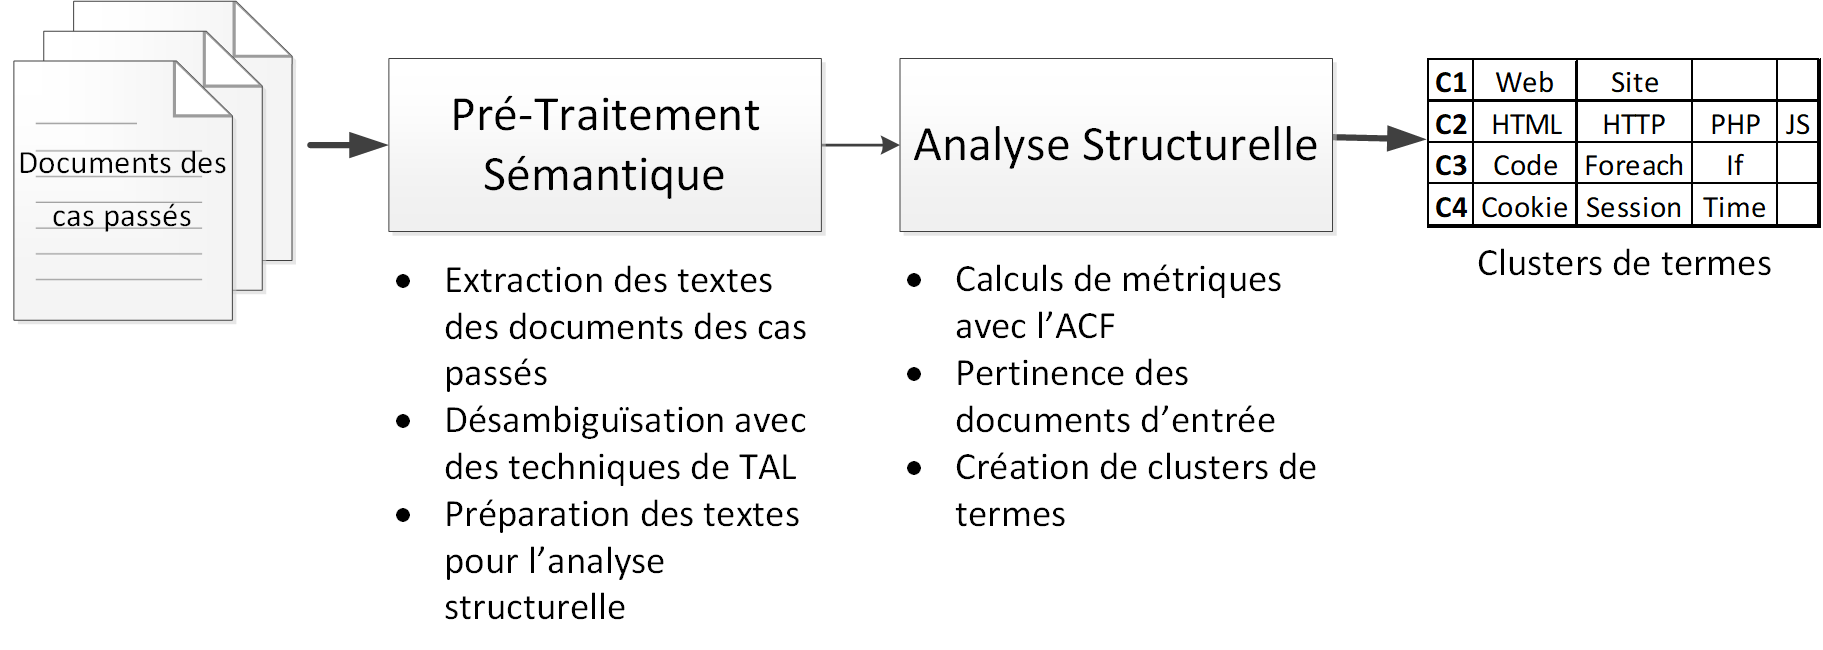
\includegraphics[width=3in]{3-Methode-CREA/images/schema_general.png}
\centerline{  % FORCE FIGURE OUTSIDE THE MARGIN !!! BUT STILL CENTERING !!!
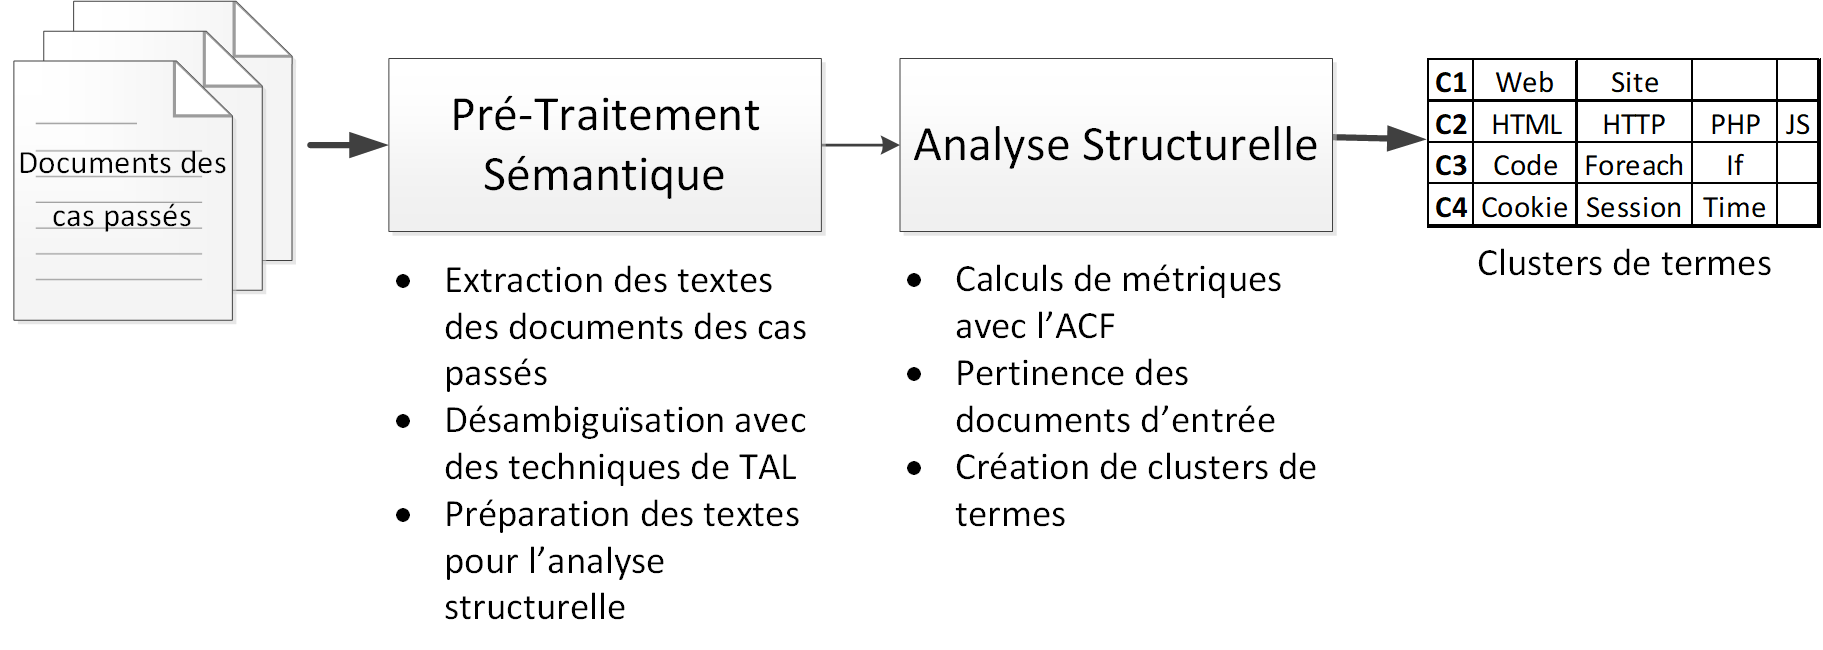
\includegraphics[scale=0.7]{3-Methode-CREA/images/schema_general.png}
}
\caption{Les deux principales phases de la méthode CREA}
\label{figure:3-MethodeGenerale}
\end{figure}
%\end{figure*} % Figure flottante
% To use it : fig~\ref{label}

\bigskip

La phase de pré-traitement sémantique (PI) est divisée en cinq étapes qui s'appuient sur plusieurs techniques de traitement automatique du langage présentées en section~\ref{subsection:Contexte:TechniquesUtilisees:TAL}.
Ces étapes permettent d'extraire les termes des documents sélectionnés, puis de lier ces termes à des entités reconnues dans des bases de connaissances grâce à une étape de désambiguïsation.
Ces bases de connaissances permettent de standardiser les entités manipulées dans l'ensemble du corpus de textes en faisant abstraction des synonymes mais également des langues utilisées dans les documents.
À l'issue de ces cinq étapes, une liste de termes standardisés est générée pour chacun des documents.
Les traitements suivants s'appuient soit sur ce format en \textit{liste}, soit sur un format en \textit{matrice d'occurrences} de termes dans des documents comme illustré sur la figure~\ref{figure:3-MethodeGenerale-PI-outputs}.
Appliqué au cas de l'enseignement il s'agit donc de générer, pour chacun des supports de cours sélectionnés, une liste de termes standardisés et reconnus dans des bases de connaissances représentant les notions abordées dans le cours.


%\begin{figure*} % Figure flottante
\begin{figure}[ht]
\centering
\centerline{  % FORCE FIGURE OUTSIDE THE MARGIN !!! BUT STILL CENTERING !!!
% scale = 0.6   1 OK dans certaines circonstances
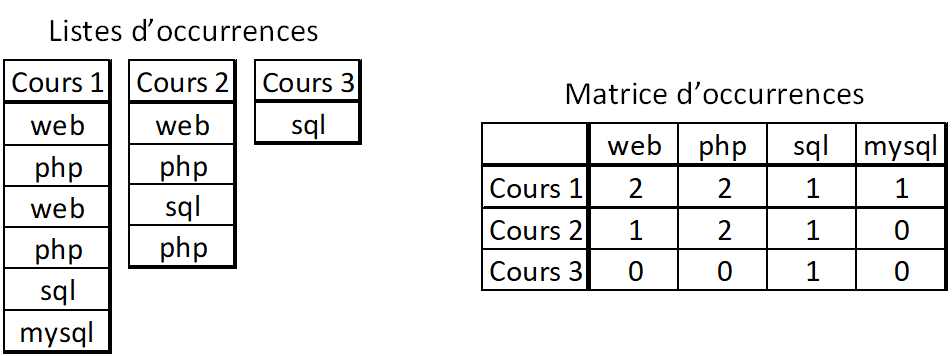
\includegraphics[scale=0.85]{3-Methode-CREA/images/0-fonctionnement-general/listes-et-matrice.png}
}
\caption{Exemple de listes et de matrice d'occurrences de termes générées à l'issue de la phase de pré-traitement sémantique (PI)}
\label{figure:3-MethodeGenerale-PI-outputs}
\end{figure}
%\end{figure*} % Figure flottante
% To use it : fig~\ref{label}

\bigskip

La phase d'analyse structurelle (PII) est divisée en trois grandes étapes qui s'appuient sur l'analyse de concepts formels, présentée en section~\ref{subsection:Contexte:TechniquesUtilisees:ACF}, et les méthodes de clustering, présentées en section~\ref{subsection:Contexte:TechniquesUtilisees:Clustering}.
Ces étapes permettent d'analyser les documents et les termes les composant, afin d'évaluer leur pertinence et d'en extraire les regroupements de termes les plus utiles à l'utilisateur.
Dans le domaine de l'enseignement, il s'agit donc de générer des métriques évaluant la qualité de la composition des supports de cours entre eux, afin de permettre à l'enseignant de supprimer des supports qui ne conviennent pas à ses exigences ou éventuellement des notions qu'il ne souhaite pas aborder, et pouvoir en extraire des clusters de termes représentant une structure de cours réutilisable.
Par exemple, si un enseignant souhaite construire un cours de développement web à l'aide de PHP en s'appuyant sur une dizaine de supports de cours, mais dont l'un traite en fait de Java, un graphique lui permettra de constater qu'un des supports de cours insérés est hors sujet et doit être vérifié pour éventuellement le retirer.
La figure~\ref{figure:3-MethodeGenerale-PII-output-graphe} montre que les supports C6 et CJA sont beaucoup plus éloignés des autres, et devraient être vérifiés manuellement.
Ensuite, lorsque le corpus de documents est considéré par l'enseignant comme convenable, des clusters peuvent être générés selon le nombre de séances souhaité.
La figure~\ref{figure:3-MethodeGenerale-PII-output-clusters} montre huit clusters générés à partir de plusieurs supports de cours de PHP (les clusters ne sont pas ordonnés), l'enseignant peut ainsi s'appuyer dessus pour préparer ses huit séances de cours.

%\begin{figure*} % Figure flottante
\begin{figure}[ht]
\centering
\centerline{  % FORCE FIGURE OUTSIDE THE MARGIN !!! BUT STILL CENTERING !!!
% scale = 0.6
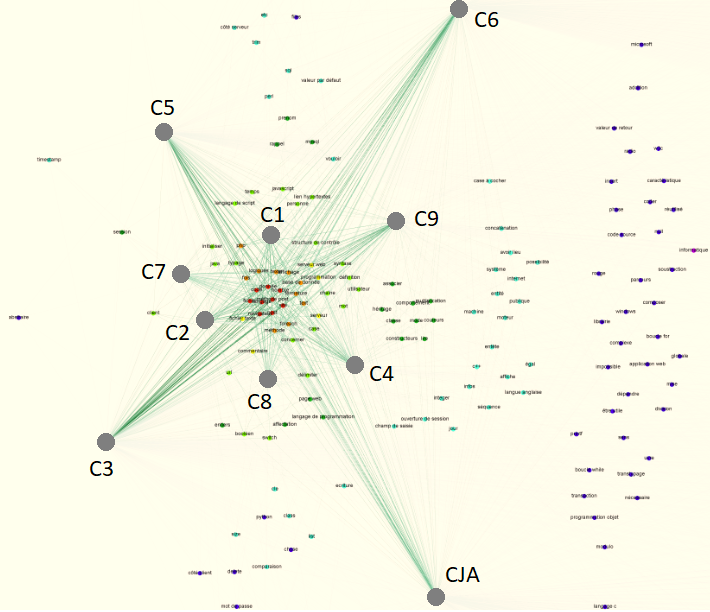
\includegraphics[scale=0.45]{3-Methode-CREA/images/0-fonctionnement-general/graphe-impact-mutuel.png}
}
\caption{Exemple de graphe d'impact mutuel explicitant que les supports C6 et CJA sont éloignés des autres}
\label{figure:3-MethodeGenerale-PII-output-graphe}
\end{figure}
%\end{figure*} % Figure flottante
% To use it : fig~\ref{label}

%\begin{figure*} % Figure flottante
\begin{figure}[ht]
\centering
\centerline{  % FORCE FIGURE OUTSIDE THE MARGIN !!! BUT STILL CENTERING !!!
% scale = 0.6
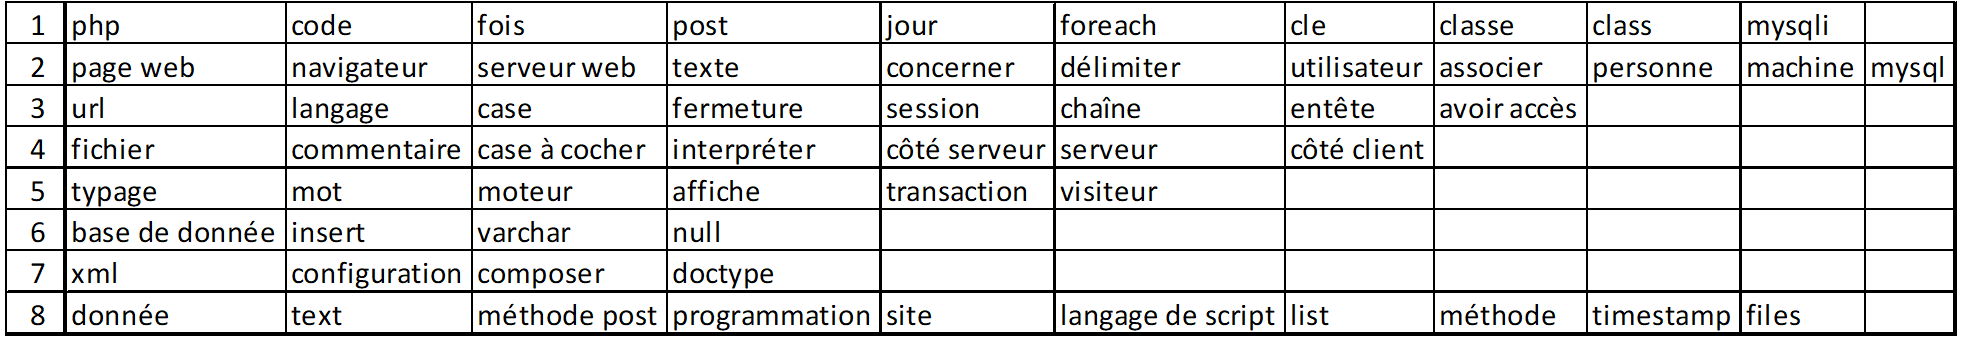
\includegraphics[scale=0.65]{3-Methode-CREA/images/0-fonctionnement-general/8-clusters.png}
}
\caption{Exemple de huit clusters générés avec la méthode CREA pour huit séances à partir de supports de cours sur PHP}
\label{figure:3-MethodeGenerale-PII-output-clusters}
\end{figure}
%\end{figure*} % Figure flottante
% To use it : fig~\ref{label}

\bigskip

La figure~\ref{figure:3-MethodeGeneraleFinale} explicite les étapes des deux phases tout en indiquant les données générées au fur et à mesure.
Comme indiqué précédemment, on observe que la première phase se concentre explicitement sur la préparation des documents fournis en entrée, afin de produire une matrice représentant l'ensemble des documents sélectionnés et les termes les composants.
La deuxième phase analyse en profondeur cette matrice pour en extraire des métriques qui servent à aider l'utilisateur à comprendre les données qu'il manipule et améliorer la qualité de sa base documentaires, le tout pour générer une structure réutilisable issue d'une liste de clusters de termes résumant ces documents.


%\begin{figure*} % Figure flottante
\begin{figure}[ht!]
\centering
%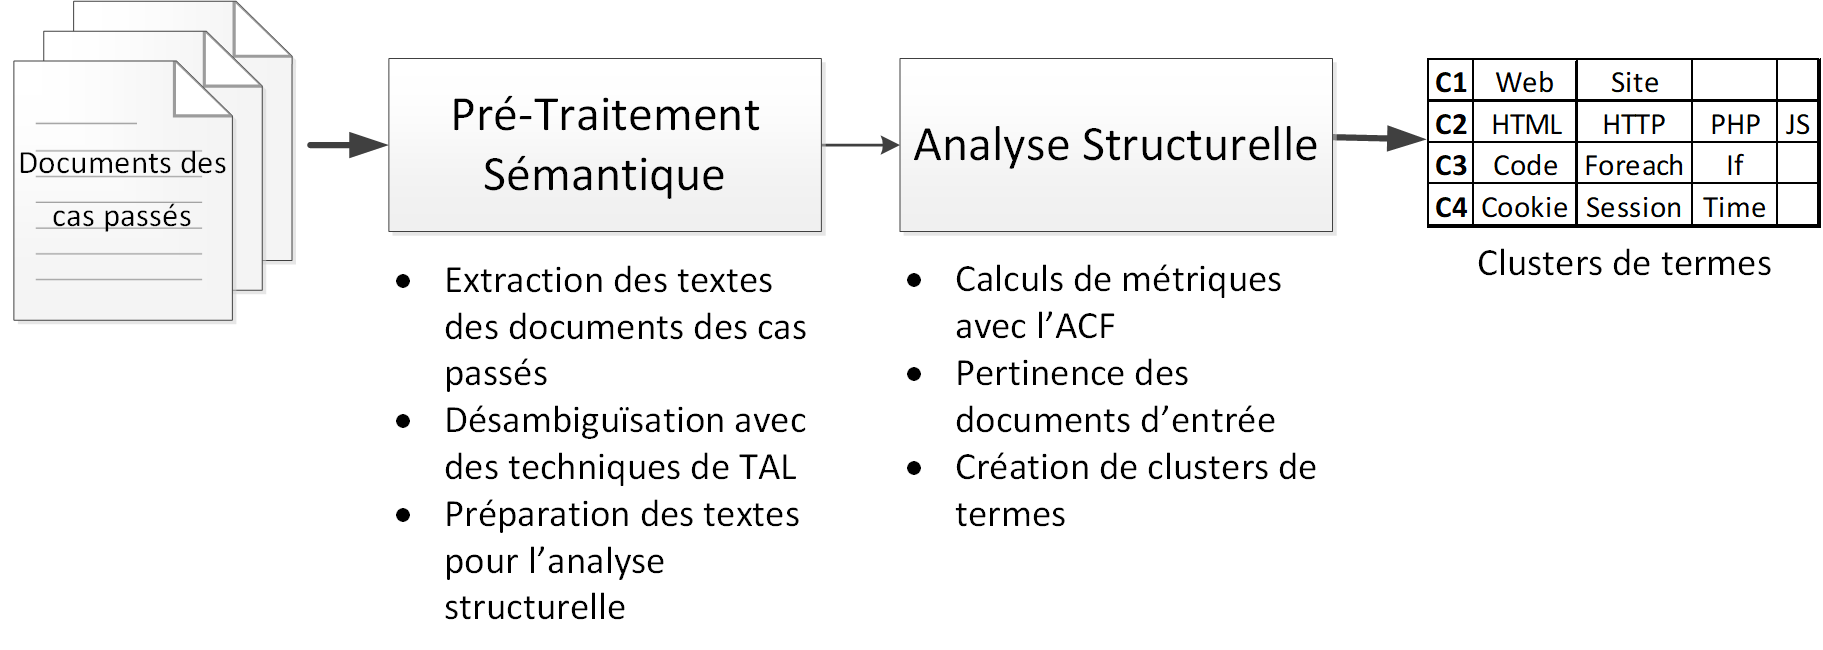
\includegraphics[width=3in]{3-Methode-CREA/images/schema_general.png}
\centerline{  % FORCE FIGURE OUTSIDE THE MARGIN !!! BUT STILL CENTERING !!!
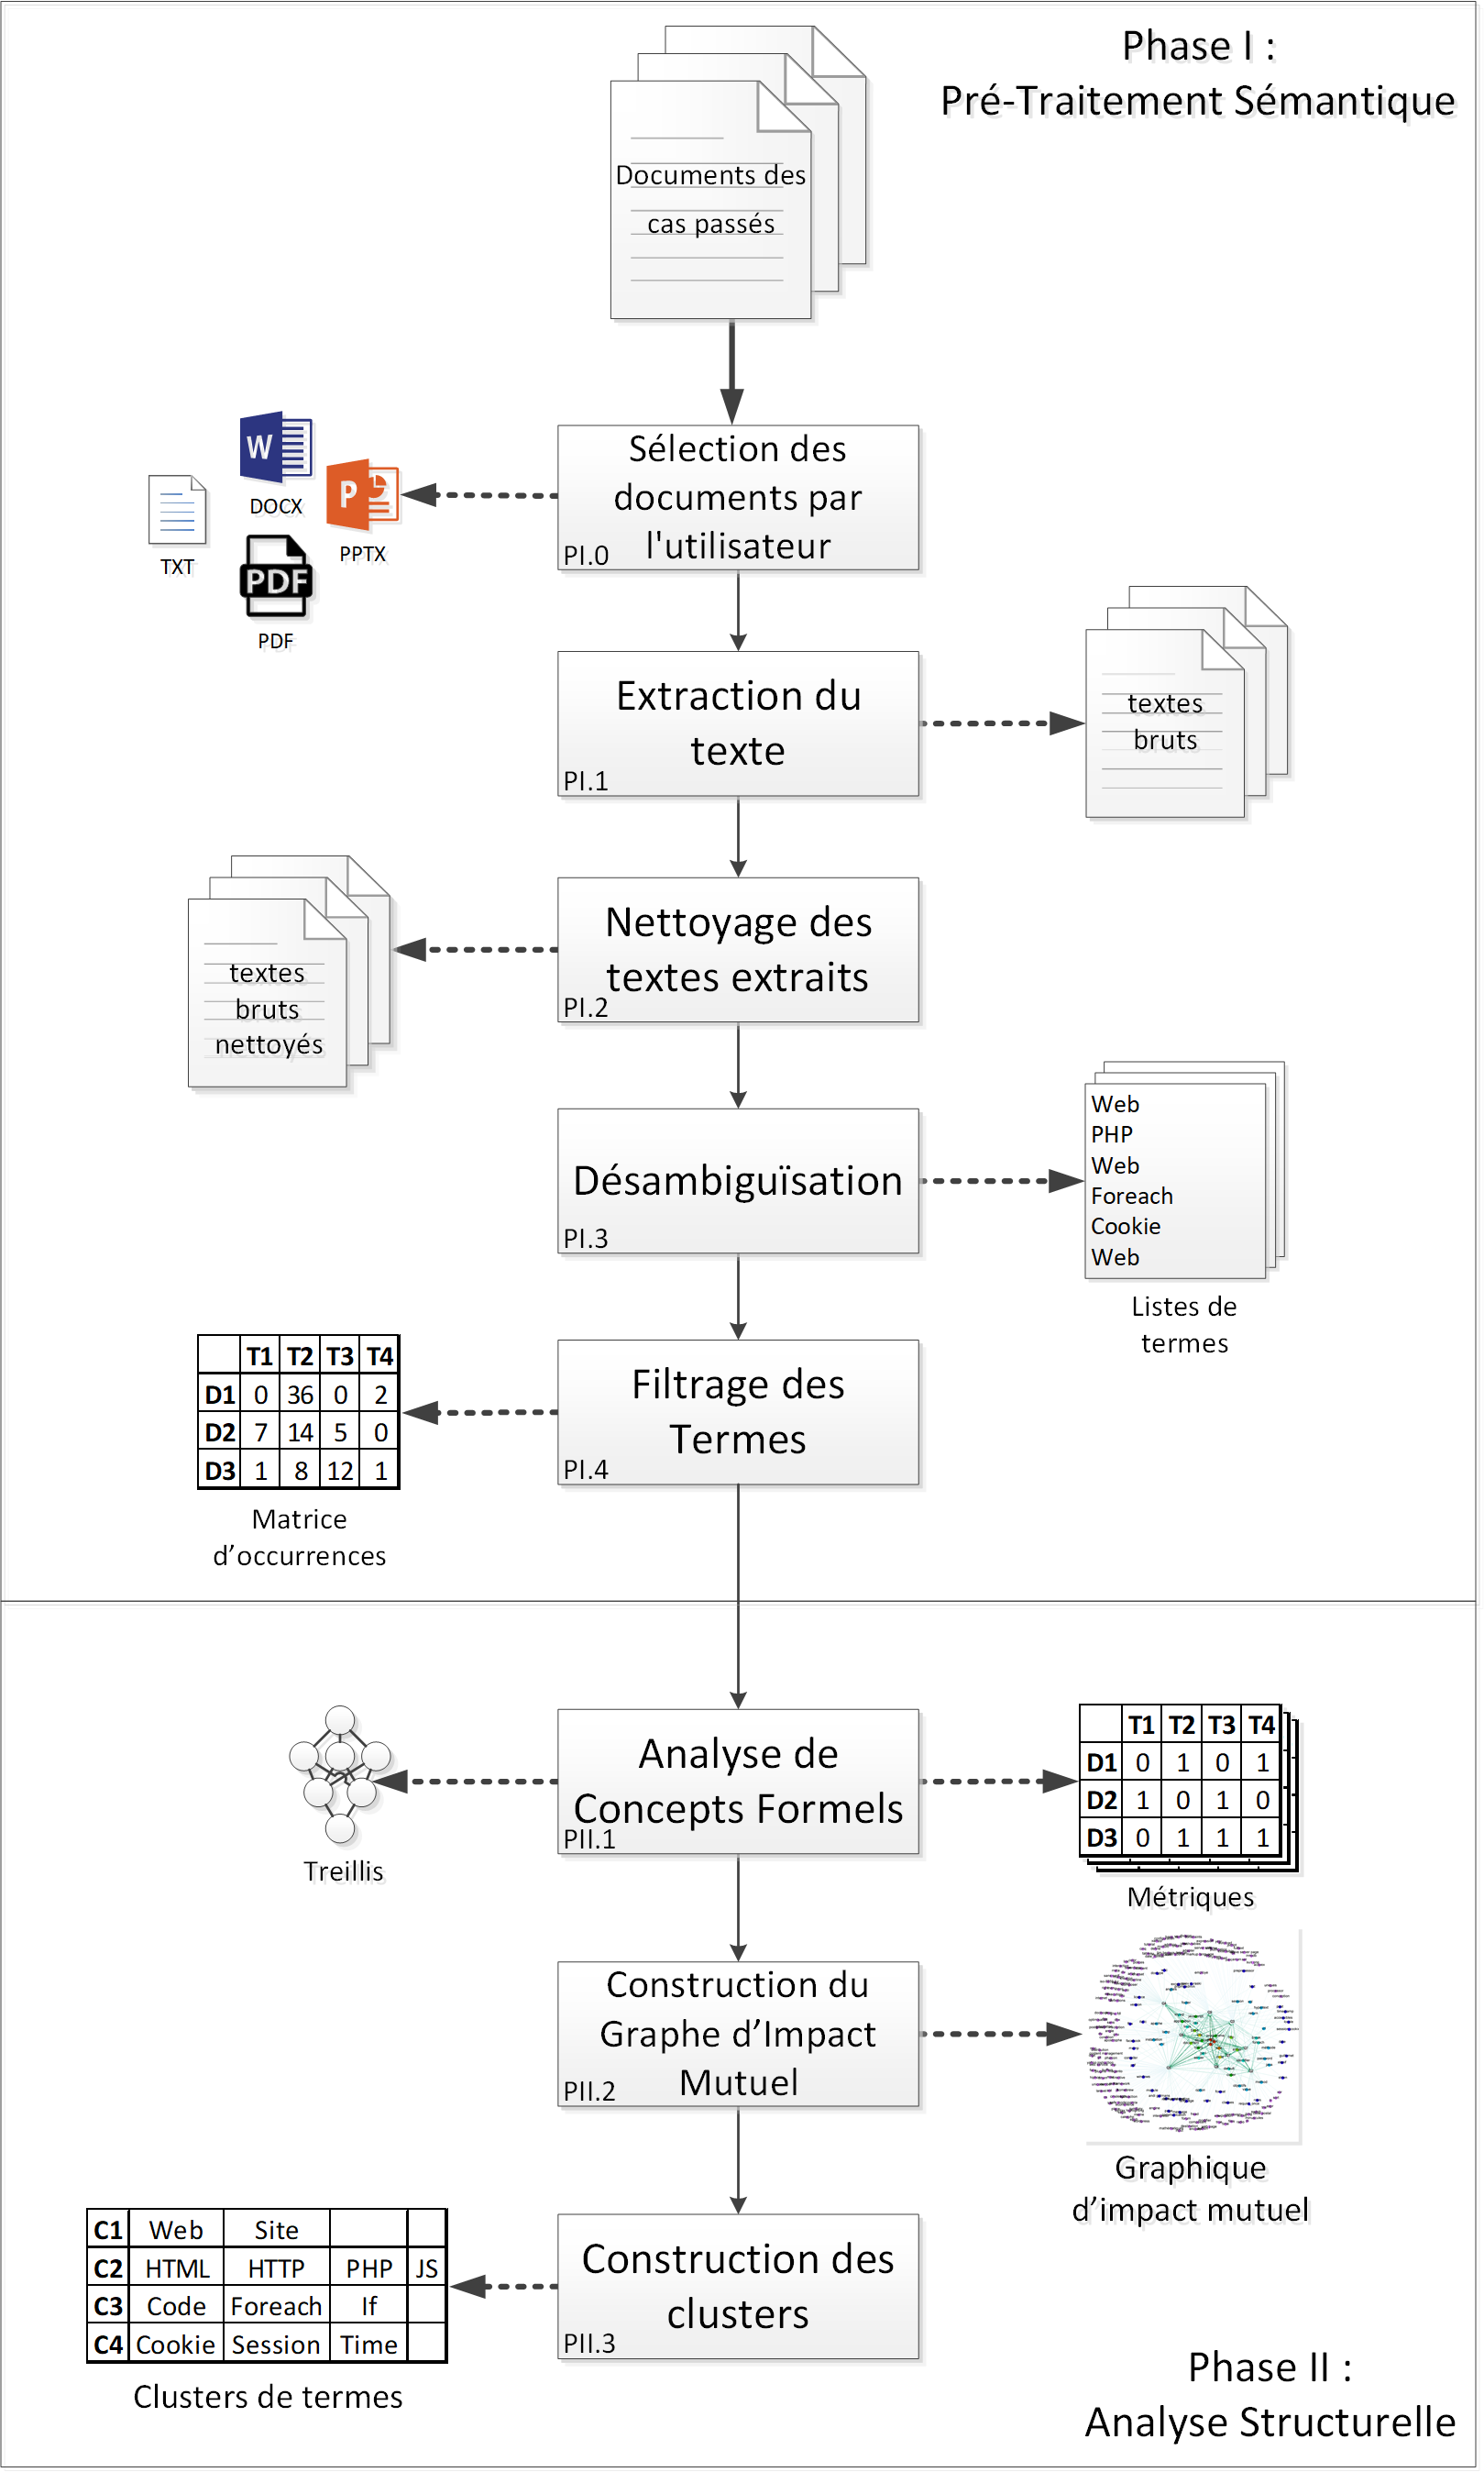
\includegraphics[scale=0.6]{3-Methode-CREA/images/schema_final.png}
}
\caption{Les deux phases détaillées de la méthode CREA}
\label{figure:3-MethodeGeneraleFinale}
\end{figure}
%\end{figure*} % Figure flottante
% To use it : fig~\ref{label}



%%%%%%%%%%%%%%%%%%%%%%%%%%%%%%%%%%%%%%%%%%%%%%%%%%%%%%%%%%%%%%%%%%%%%%%%%%%%%%%%%%%%%%%%%%
%%%%%%%%%%%%%%%%%%%%%%%%%%%%%%%%%%%%%%%%%%%%%%%%%%%%%%%%%%%%%%%%%%%%%%%%%%%%%%%%%%%%%%%%%%
%%%%%%%%%%%%%%%%%%%%%%%%%%%%%%%%%%%%%%%%%%%%%%%%%%%%%%%%%%%%%%%%%%%%%%%%%%%%%%%%%%%%%%%%%%
%%%%%%%%%%%%%%%%%%%%%%%%%%%%%%%%%%%%%%%%%%%%%%%%%%%%%%%%%%%%%%%%%%%%%%%%%%%%%%%%%%%%%%%%%%
%%%%%%%%%%%%%%%%%%%%%%%%%%%%%%%%%%%%%%%%%%%%%%%%%%%%%%%%%%%%%%%%%%%%%%%%%%%%%%%%%%%%%%%%%%
%%%%%%%%%%%%%%%%%%%%%%%%%%%%%%%%%%%%%%%%%%%%%%%%%%%%%%%%%%%%%%%%%%%%%%%%%%%%%%%%%%%%%%%%%%

%%%%%%%%%%%%%%%%%%%%%%%%%%%%%%%%%%%%%%%%%%%%
\clearpage % Clean for pictures and tables %
\newpage   % Clean for pictures and tables %
%%%%%%%%%%%%%%%%%%%%%%%%%%%%%%%%%%%%%%%%%%%%

%%%%%%%%%%%%%%%%%%%%%%%%%%%%%%%%%%%%%%%%%%%%%%%%%%%%%%%%%%%%%%%%%%%%%%%%%%%%%%%%%%%%%%%%%%
%%%%%%%%%%%%%%%%%%%%%%%%%%%%%%%%%%%%%%%%%%%%%%%%%%%%%%%%%%%%%%%%%%%%%%%%%%%%%%%%%%%%%%%%%%
%%%%%%%%%%%%%%%%%%%%%%%%%%%%%%%%%%%%%%%%%%%%%%%%%%%%%%%%%%%%%%%%%%%%%%%%%%%%%%%%%%%%%%%%%%
%%%%%%%%%%%%%%%%%%%%%%%%%%%%%%%%%%%%%%%%%%%%%%%%%%%%%%%%%%%%%%%%%%%%%%%%%%%%%%%%%%%%%%%%%%
%%%%%%%%%%%%%%%%%%%%%%%%%%%%%%%%%%%%%%%%%%%%%%%%%%%%%%%%%%%%%%%%%%%%%%%%%%%%%%%%%%%%%%%%%%
%%%%%%%%%%%%%%%%%%%%%%%%%%%%%%%%%%%%%%%%%%%%%%%%%%%%%%%%%%%%%%%%%%%%%%%%%%%%%%%%%%%%%%%%%%

\section{Pré-traitement sémantique : extraction des termes}
\label{section:CREA:PI-AnalyseSemantique}

La première phase (PI) de la méthode CREA, le pré-traitement sémantique, a pour objectif d'extraire une liste de termes à partir de documents fournis en entrée, et de les rassembler sous forme d'une matrice d'occurrences afin de les organiser plus tard sous forme de clusters.
Dans le contexte de l'enseignement supérieur, ces termes représentent les notions abordées dans les supports de cours fournis en entrée.
Cette première phase se déroule en cinq étapes successives illustrées par la figure~\ref{figure:3-I-PreTraitementSemantique}.

%\begin{figure*} % Figure flottante
\begin{figure}[ht]
\centering
\centerline{  % FORCE FIGURE OUTSIDE THE MARGIN !!! BUT STILL CENTERING !!!
% 0.49
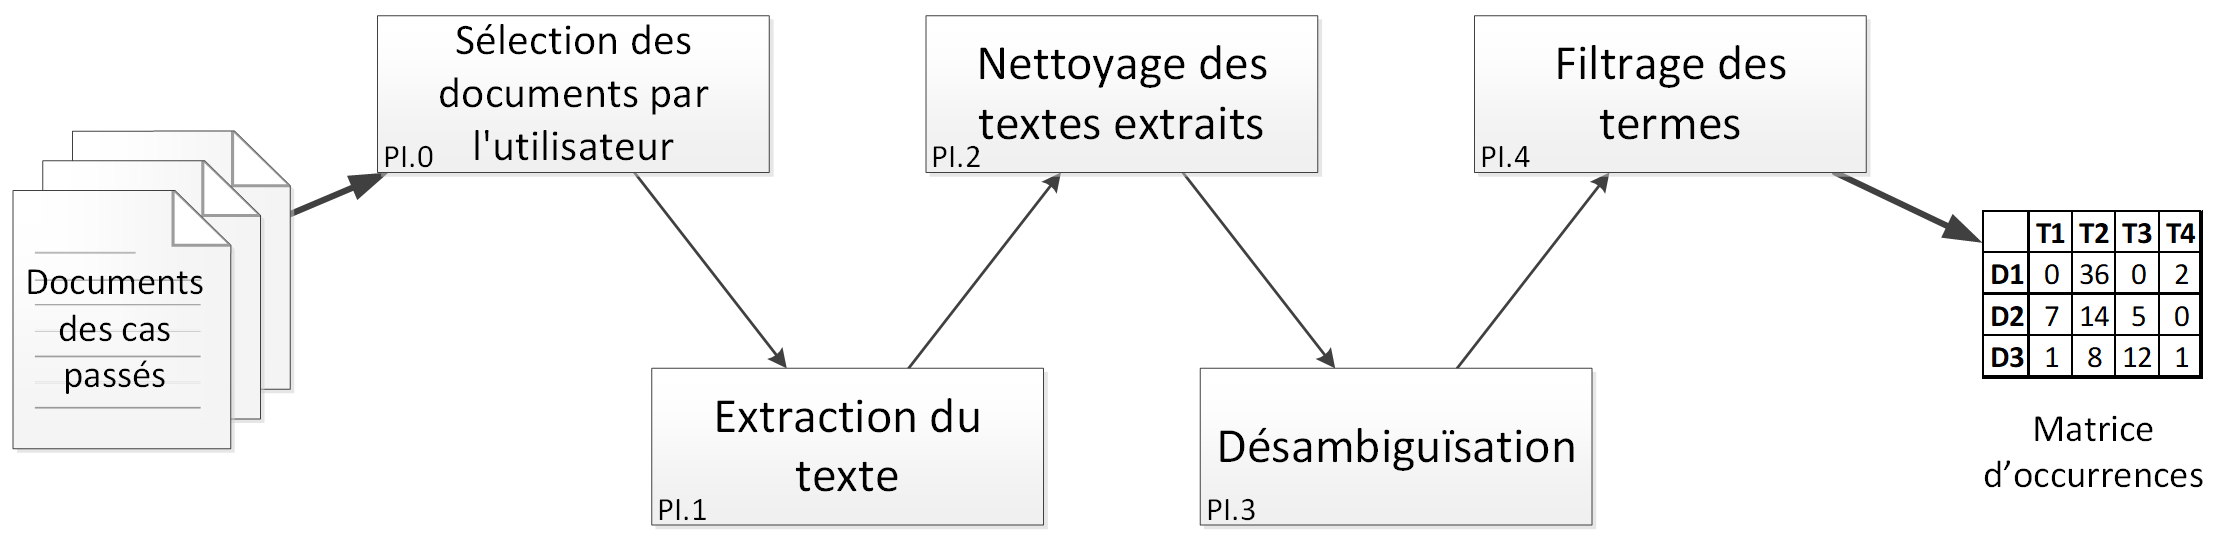
\includegraphics[scale=0.55]{3-Methode-CREA/images/schema_pre-traitement_semantique_ESCALIER.png}
}
\caption{Les étapes de la phase de pré-traitement sémantique}
\label{figure:3-I-PreTraitementSemantique}
\end{figure}
%\end{figure*} % Figure flottante
% To use it : fig~\ref{label}

\begin{itemize}
\item Sélection des documents par l'utilisateur (PI.0) : Tout d'abord, l'enseignant sélectionne des supports de cours dont les titres lui semblent pertinents et dont le contenu est majoritairement composé de texte.
\item Extraction du texte (PI.1) : Une étape d'extraction du texte s'appuie sur la reconnaissance optique de caractères (ou \textit{OCR}) pour pouvoir transformer les supports de cours en texte brut dont les termes seront reconnaissables par la suite.
\item Nettoyage des textes extraits (PI.2) : Les textes extraits sont ensuite nettoyés afin de supprimer les caractères mal reconnus ainsi que les classes grammaticales de mots dont la présence augmente le bruit dans la suite des traitements.
\item Désambiguïsation (PI.3) : Les textes nettoyés sont ensuite désambiguïsés et suivent un traitement d'annotation sémantique afin d'en extraire les termes directement liés à des entités reconnues dans des bases de connaissances.
\item Filtrage des Termes (PI.4) : Enfin, les termes dont le score de désambiguïsation est trop faible sont retirés, afin de ne garder que les termes dont le sens est reconnu avec suffisamment de confiance.
\end{itemize}



\subsection{Sélection des documents par l'utilisateur (PI.0)}
\label{subsection:CREA:SelectionDocuments}

La \textit{sélection des documents par l'utilisateur} est l'étape préliminaire où l'utilisateur sélectionne des documents selon ses exigences.
Le but de cette étape est de choisir les documents aptes à être analysés avec les techniques de TAL.
Afin de construire le corpus documentaire le plus adapté au sujet visé et le plus propice à la réutilisation, trois exigences sont à respecter concernant les documents : le contenu doit être en relation avec le sujet de cours visé (le titre et quelques extraits du contenu peuvent donner un indice de pertinence), le contenu doit être suffisamment conséquent (un document trop court n'apportera que peu de notions, ni ne contiendra suffisamment de relations entre ces notions pour produire un résultat utile), et enfin, le contenu doit être principalement au format textuel.
En effet, le traitement de formats spécifiques de représentation du contenu (par exemple des images, des tableaux, des listings de code, etc) est hors du cadre de ces travaux, et nous en discutons dans la conclusion.

\bigskip

Dans le contexte de l'enseignement supérieur, les supports de cours sous forme de manuscrits ou de diapositives contenant du texte, sont adaptés, tout comme les articles de recherche.


\subsection{Extraction du texte (PI.1)}
\label{subsection:CREA:PI.2-extraction}

L'\textit{extraction du texte} vise à transformer les formats variés d'encodage des textes, en texte brut.
Le but de cette étape est d'extraire les textes des documents insérés.
Les documents dont le texte est déjà numérisé sous forme de texte brut peuvent être utilisés tels quels.
En revanche, les textes imprimés ou les scans sous forme d'images ont besoin de passer par des outils de reconnaissance optique de caractères.
Nous ne détaillerons pas ces opérations étant donné que les nouveaux supports sont principalement produits et stockés sous format numérique, et que de plus en plus de projets de numérisation des bibliothèques sont lancés depuis les années 1990~\cite{brosset:dumas-01376071}.
Il existe encore d'autres formats numériques qui encapsulent les textes (PDF, DOCX, ...).
Certains outils permettent d'extraire et reconstituer ces textes encapsulés, comme PDFtoText~\footnote{ \href{https://www.xpdfreader.com/pdftotext-man.html}{Projet PDFtoText} }.


\subsection{Nettoyage des textes extraits (PI.2)}
\label{subsection:CREA:PI.3-nettoyage}

Le \textit{Nettoyage des textes extraits} a pour objectif d'améliorer la qualité des données en les nettoyant (l'équivalent du \textit{data cleansing} en anglais), c'est-à-dire de supprimer les caractères non-affichables ainsi que les mots inutiles pour les traitements suivants.
L'extraction du texte brut des documents générant parfois des coquilles dans les textes, le but de cette étape est d'améliorer la qualité des données pour les traitements automatiques suivants.
La figure~\ref{figure:3-I-3-NettoyageDonnees-ProblemeOCR} illustre en pratique certaines difficultés des logiciels de reconnaissance optique de caractères dans un cas extrême, où un nettoyage du texte brut est requis.
Des informations peu pertinentes pour le cas présent peuvent se retrouver en grande quantité dans le texte (par exemple les pronoms et articles fréquemment employés, ou les en-têtes sur chaque page).
Afin de limiter l'impact sur les traitements suivants, cette étape se fait relativement tôt dans la méthode.

\bigskip

Pour notre implémentation, nous avons choisi de supprimer certaines classes grammaticales de mots, comme présenté dans le tableau~\ref{table:3-I-3-NettoyageDonnees-Classesgrammaticales}.
Les résultats de l'extraction peuvent varier selon les documents insérés et peuvent potentiellement être améliorés avec un nettoyage manuel ultérieur.

\bigskip

Afin d'étiqueter puis filtrer les classes grammaticales, nous utilisons TreeTagger~\cite{schmid1994probabilistic}\cite{Schmid95improvementsin}.
Le domaine étudié dans nos expériences étant l'informatique, nous avons choisi de conserver certaines classes qui pourraient paraitre superflues.
Par exemple, la ponctuation est nécessaire pour pouvoir parler des différences de traitement par les guillemets simples (~\textquotesingle~) et doubles (~{\tt\textquotedbl}~) dans certains langages de programmation.
En outre, l'absence de certaines prépositions et certains adjectifs entraîne des résultats assez négatifs dans les traitements suivants (\og \textit{base~de~données} \fg étant transformé en \og \textit{base} \fg, ce qui fait perdre tout son sens au terme).
La liste des classes TreeTagger que nous avons conservées ou supprimées pour la langue française est présentée dans le tableau~\ref{table:3-I-3-NettoyageDonnees-Classesgrammaticales}.

\bigskip

\vfill
\hspace{0pt}

\begin{figure}[ht]
\centering
\centerline{  % FORCE FIGURE OUTSIDE THE MARGIN !!! BUT STILL CENTERING !!!   scale=0.65
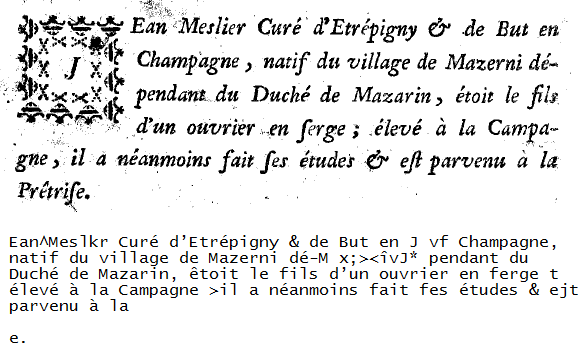
\includegraphics[scale=1]{3-Methode-CREA/images/1-pre-traitement-semantique/exemple_probleme_OCR.png}
}
\caption{Exemple d'un cas difficile pour un logiciel de reconnaissance optique de caractères (extrait du Testament de Jean Meslier - 1762)}
\label{figure:3-I-3-NettoyageDonnees-ProblemeOCR}
\end{figure}

\hspace{0pt}
\vfill

%\newpage
\bigskip


\begin{table}[ht]
\centering
\begin{tabular}{| l | l |}
\hline
\textbf{Conservées} 				& \textbf{Supprimées} \\
\hline
abréviation ($ABR$) 					& adverbe ($ADV$) \\ \hline
adjectif ($ADJ$)  						& article ($DET{:}ART$) \\ \hline
interjection ($INT$) 					& pronom possessif ($DET{:}POS$) \\ \hline
nom propre et mots inconnus ($NAM$) 	& conjonction ($KON$) \\ \hline
nom commun ($NOM$)						& pronom ($PRO$) \\ \hline
numéro ($NUM$)							& pronom démonstratif ($PRO{:}DEM$) \\ \hline
préposition ($PRP$)						& pronom indéfini ($PRO{:}IND$) \\ \hline
ponctuation ($PUN$)						& pronom personnel ($PRO{:}PER$) \\ \hline
ponctuation de citation ($PUN{:}cit$)	& pronom possessif ($PRO{:}POS$) \\ \hline
point final ($SENT$)					& pronom relatif ($PRO{:}REL$) \\ \hline
symbole ($SYM$)							& préposition plus article ($PRP{:}det$) \\ \hline
verbe - conditionnel ($VER{:}cond$)		& \\ \hline
verbe - futur ($VER{:}futu$)			& \\ \hline
verbe - impératif ($VER{:}impe$)		& \\ \hline
verbe - imparfait ($VER{:}impf$)		& \\ \hline
verbe - infinitif ($VER{:}infi$)		& \\ \hline
verbe - participe passé ($VER{:}pper$)	& \\ \hline
verbe - participe présent ($VER{:}ppre$)		& \\ \hline
verbe - présent ($VER{:}pres$)					& \\ \hline
verbe - passé simple ($VER{:}simp$)				& \\ \hline
verbe - imparfait du subjonctif ($VER{:}subi$)	& \\ \hline
verbe - présent subjonctif ($VER{:}subp$)		& \\ \hline
\end{tabular}
\caption{Classes grammaticales conservées ou supprimées}
\label{table:3-I-3-NettoyageDonnees-Classesgrammaticales}
\end{table}




%%%%%%%%%%%%%%%%%%%%%%%%%%%%%%%%%%%%%%%%%%%%
\clearpage % Clean for pictures and tables %
\newpage   % Clean for pictures and tables %
%%%%%%%%%%%%%%%%%%%%%%%%%%%%%%%%%%%%%%%%%%%%

\subsection{Désambiguïsation (PI.3)}
\label{subsection:CREA:PI.4-Desambiguisation}

La \textit{désambiguïsation} est l'étape clé du pré-traitement sémantique.
En effet, la phase suivante d'analyse structurelle manipulant des documents et les termes communs entre ces documents, il est nécessaire de standardiser ces termes en retrouvant les concepts (au sens du triangle sémiotique~\cite{zargayouna2015recherche}) qui leurs sont attachés.
Cette étape permet donc à la fois de désambiguïser les termes selon le contexte, mais aussi de les lier à un concept particulier.
Ainsi, les problèmes de polysémie\footnote{\og \textit{La plupart [des mots] sont polysémiques, c'est-à-dire pourvus de plusieurs sens} \fg~\cite{goosse2016bon} } et de synonymie\footnote{\og \textit{Les synonymes sont des mots qui, appartenant à la même classe grammaticale, ont à peu près la même signification} \fg~\cite{goosse2016bon} } sont résolus grâce au contexte du document.

À l'issue de cette étape, une liste de termes désambiguïsés avec l'identifiant unique de concept associé est fournie.

\bigskip

Nous avons implémenté cette étape avec BabelFy~\cite{moro2014entity}\cite{moro2014multilingual}, un outil de désambiguïsation et d'annotation sémantique, lié à BabelNet~\cite{navigli2012babelnet}, un réseau sémantique multilingue manipulant des concepts et des entités nommées lié à WordNet~\cite{miller1995wordnet} et Wikipedia.
BabelFy est capable de déduire quel entité nommée ou concept est manipulé pour chacun des termes, et ce dans une multitude de langues.
Son autre atout réside dans son lien avec BabelNet, et donc l'encyclopédie Wikipedia : les concepts et entités de la vie courante (technologies, produits commerciaux, ...) sont reconnaissables dans les textes, y compris lorsque ceux-ci sont spécifiques à un domaine bien particulier.
BabelFy cherche donc les liens les plus probables entre un terme et un concept ou une entité nommée, puis il indique l'identifiant unique retenu et différents scores liés à ses traitements.

\bigskip

La figure~\ref{figure:3-I-4-Desambiguisation-BabelFyGUI} illustre parfaitement l'utilité de BabelFy par rapport à d'autres outils plus traditionnels concernant les termes particuliers à certains domaines.
On peut voir dans le formulaire d'entrée que le terme \og \textit{PHP} \fg est reconnu par le navigateur web, mais pas \og \textit{MySQLi} \fg (le correcteur orthographique intégré le faisant remarquer).
Cependant, grâce à son accès à une base de connaissances suffisamment large, BabelFy arrive à reconnaître l'extension peu connue des non-initiés qu'est \og \textit{MySQLi} \fg .
Dans le cadre de cours d'informatique, tous les termes clés sont donc automatiquement extraits des supports de cours insérés, en plus d'être identifiés de façon unique.


%\begin{figure*} % Figure flottante
\begin{figure}[ht]
\centering
%\includegraphics[width=3in]{images/VerySmallModels_text.png}
%%\includegraphics[scale=0.6]{images/VerySmallModels_text.png}
\centerline{  % FORCE FIGURE OUTSIDE THE MARGIN !!! BUT STILL CENTERING !!!
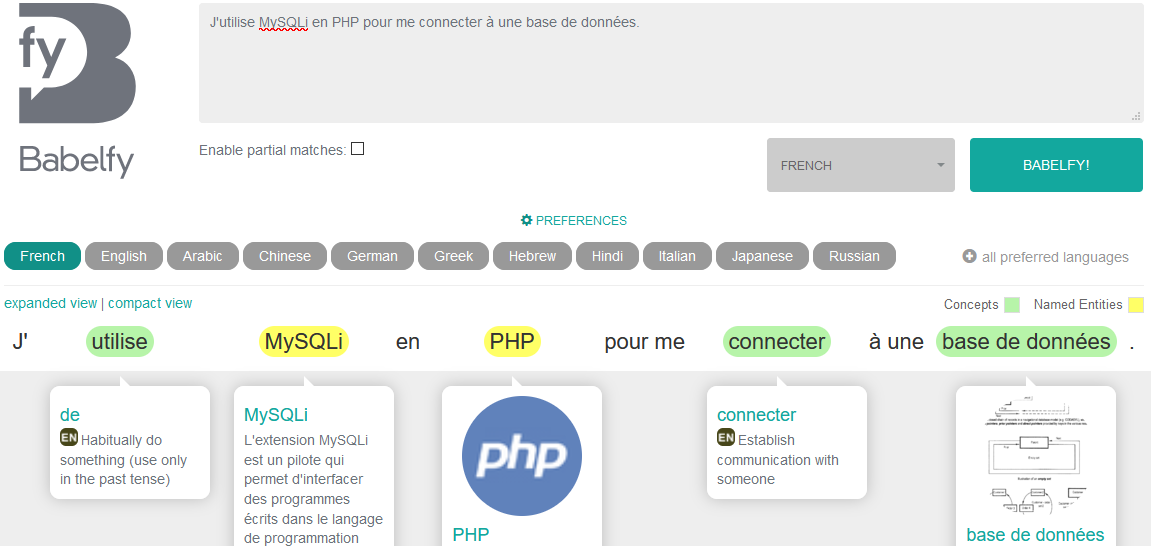
\includegraphics[scale=0.54]{3-Methode-CREA/images/1-pre-traitement-semantique/desambiguisation-GUI.png}
}
\caption{Exemple de désambiguïsation et d'annotation sémantique avec BabelFy}
\label{figure:3-I-4-Desambiguisation-BabelFyGUI}
\end{figure}
%\end{figure*} % Figure flottante
% To use it : fig~\ref{label}

\bigskip

Parmi les choix de paramétrage de BabelFy, nous avons opté pour des correspondances exactes (\textit{MatchingType.EXACT\_MATCHING}) et les candidats obtenant les meilleurs scores (\textit{ScoredCandidates.TOP}), afin d'obtenir les sens dont BabelFy est le plus sûr.
BabelFy n'autorisant pas des textes de plus de $ 10.000 $ caractères, les textes transmis sont équitablement découpés pour distribuer autant que possible le plus de caractères dans le moins de groupes possibles, tout en respectant la limite et en conservant entiers les mots aux extrémités.
L'intérêt de transmettre de grands groupes de mots est que le contexte est mieux compris par BabelFy, et donc la qualité de ses résultats en est améliorée.
L'essentiel étant d'éviter l'utilisation d'une simple division euclidienne qui ne transmettrait que dans un seul cas des groupes parfaitement égaux, et inversement, dans beaucoup d'autres cas le dernier groupe serait relativement petit.


%%%%%%%%%%%%%%%%%%%%%%%%%%%%%%%%%%%%%%%%%%%%
%\clearpage % Clean for pictures and tables %
%\newpage   % Clean for pictures and tables %
%%%%%%%%%%%%%%%%%%%%%%%%%%%%%%%%%%%%%%%%%%%%

\bigskip

\subsection{Filtrage des termes (PI.4)}
\label{subsection:CREA:PI.5-FiltrageTermes}

La dernière étape, le \textit{filtrage des termes}, consiste à améliorer la qualité des listes de termes désambiguïsés en supprimant les termes hors sujet.
L'intérêt est de ne proposer à l'utilisateur que des termes en lien avec le domaine, et donc de produire des fragments contenant des termes pertinents pour le cas géré.
BabelFy met à disposition plusieurs scores suite à ses traitements.
Le score de cohérence mesure en particulier la connectivité d'un terme avec les autres termes du texte transmis~\cite{prohaska2017masterthesis} (d'où l'intérêt d'envoyer les plus grands groupes de mots possibles de façon équitable).

\bigskip

% É
Nous avons empiriquement constaté que beaucoup de termes inutiles pouvaient être facilement éliminés en fixant un score minimum de cohérence à atteindre.
Le score de cohérence correspond au niveau de connectivité du terme désambiguïsé par rapport aux autres termes du même texte fourni à BabelFy.
Les termes dont le score de cohérence est strictement supérieur à $ 0,05 $ sont conservés.
Ce score élimine malgré tout quelques occurrences de termes intéressants, mais celles-ci restent relativement faibles par rapport à la quantité de termes hors sujet.

\bigskip

À l'issue de cette étape nous obtenons pour chaque document une liste de termes désambiguïsés et en lien avec le sujet.
Ces listes sont fusionnées sous forme de matrice d'occurrences, afin d'obtenir un format utile pour la phase suivante.

Étant donné que plusieurs documents peuvent contenir les mêmes termes désambiguïsés, on crée une matrice rassemblant les occurrences des termes contenus dans chaque document.
La figure~\ref{figure:3-I-5-MatriceOccurrences} illustre une matrice d'occurrences où l'on peut voir dix documents d'entrée (Cours 1 à 10) et quatre termes (web, php, sql, mysql) avec leurs identifiants dans la base de connaissances BabelNet.
On peut voir en pratique que le terme \og \textit{php} \fg, dont l'identifiant unique est \og $bn{:}01753580n$ \fg, apparait \textit{15} fois dans le \textit{Cours 1} et \textit{53} fois dans le \textit{Cours 2}.
Cette matrice est un pré-requis pour la phase suivante appliquant l'ACF.

%\begin{figure*} % Figure flottante
\begin{figure}[ht]
\centering
%\includegraphics[width=3in]{images/VerySmallModels_text.png}
%%\includegraphics[scale=0.6]{images/VerySmallModels_text.png}
\centerline{  % FORCE FIGURE OUTSIDE THE MARGIN !!! BUT STILL CENTERING !!!
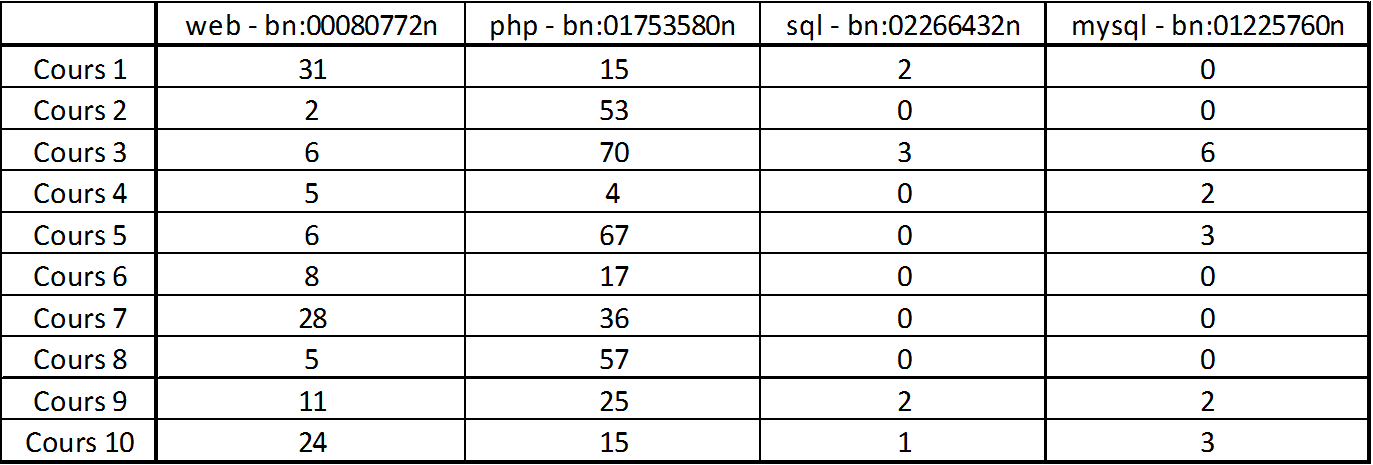
\includegraphics[scale=0.85]{3-Methode-CREA/images/1-pre-traitement-semantique/exemple_matrice_occurrences.png}
}
\caption{Exemple de matrice d'occurrences}
\label{figure:3-I-5-MatriceOccurrences}
\end{figure}
%\end{figure*} % Figure flottante
% To use it : fig~\ref{label}




%%%%%%%%%%%%%%%%%%%%%%%%%%%%%%%%%%%%%%%%%%%%%%%%%%%%%%%%%%%%%%%%%%%%%%%%%%%%%%%%%%%%%%%%%%
%%%%%%%%%%%%%%%%%%%%%%%%%%%%%%%%%%%%%%%%%%%%%%%%%%%%%%%%%%%%%%%%%%%%%%%%%%%%%%%%%%%%%%%%%%
%%%%%%%%%%%%%%%%%%%%%%%%%%%%%%%%%%%%%%%%%%%%%%%%%%%%%%%%%%%%%%%%%%%%%%%%%%%%%%%%%%%%%%%%%%
%%%%%%%%%%%%%%%%%%%%%%%%%%%%%%%%%%%%%%%%%%%%%%%%%%%%%%%%%%%%%%%%%%%%%%%%%%%%%%%%%%%%%%%%%%
%%%%%%%%%%%%%%%%%%%%%%%%%%%%%%%%%%%%%%%%%%%%%%%%%%%%%%%%%%%%%%%%%%%%%%%%%%%%%%%%%%%%%%%%%%
%%%%%%%%%%%%%%%%%%%%%%%%%%%%%%%%%%%%%%%%%%%%%%%%%%%%%%%%%%%%%%%%%%%%%%%%%%%%%%%%%%%%%%%%%%

%%%%%%%%%%%%%%%%%%%%%%%%%%%%%%%%%%%%%%%%%%%%
\clearpage % Clean for pictures and tables %
\newpage   % Clean for pictures and tables %
%%%%%%%%%%%%%%%%%%%%%%%%%%%%%%%%%%%%%%%%%%%%

%%%%%%%%%%%%%%%%%%%%%%%%%%%%%%%%%%%%%%%%%%%%%%%%%%%%%%%%%%%%%%%%%%%%%%%%%%%%%%%%%%%%%%%%%%
%%%%%%%%%%%%%%%%%%%%%%%%%%%%%%%%%%%%%%%%%%%%%%%%%%%%%%%%%%%%%%%%%%%%%%%%%%%%%%%%%%%%%%%%%%
%%%%%%%%%%%%%%%%%%%%%%%%%%%%%%%%%%%%%%%%%%%%%%%%%%%%%%%%%%%%%%%%%%%%%%%%%%%%%%%%%%%%%%%%%%
%%%%%%%%%%%%%%%%%%%%%%%%%%%%%%%%%%%%%%%%%%%%%%%%%%%%%%%%%%%%%%%%%%%%%%%%%%%%%%%%%%%%%%%%%%
%%%%%%%%%%%%%%%%%%%%%%%%%%%%%%%%%%%%%%%%%%%%%%%%%%%%%%%%%%%%%%%%%%%%%%%%%%%%%%%%%%%%%%%%%%
%%%%%%%%%%%%%%%%%%%%%%%%%%%%%%%%%%%%%%%%%%%%%%%%%%%%%%%%%%%%%%%%%%%%%%%%%%%%%%%%%%%%%%%%%%

\section{Analyse structurelle : métriques de qualité et extraction des clusters}
\label{subsection:CREA:PII-AnalyseStructurelle}

La deuxième phase (PII) de la méthode CREA, l'analyse structurelle, a pour objectif d'extraire des clusters de termes en identifiant les relations entre les termes et documents traités lors de la phase précédente.
Lors de la création des documents, des connaissances ont été mobilisées afin d'organiser de manière intelligible (connaissances tacites) des notions à transmettre (connaissances explicites) à d'autres individus.
Pour le domaine de l'enseignement, il s'agit d'identifier les liens entre les notions abordées dans les supports de cours afin de réorganiser ces notions sous forme d'un syllabus, ou plus concrètement, sous forme de clusters de termes.
Cette phase se déroule en trois étapes successives illustrées par la figure~\ref{figure:3-II-AnalyseStructurelle}.


%\begin{figure*} % Figure flottante
\begin{figure}[ht]
\centering
%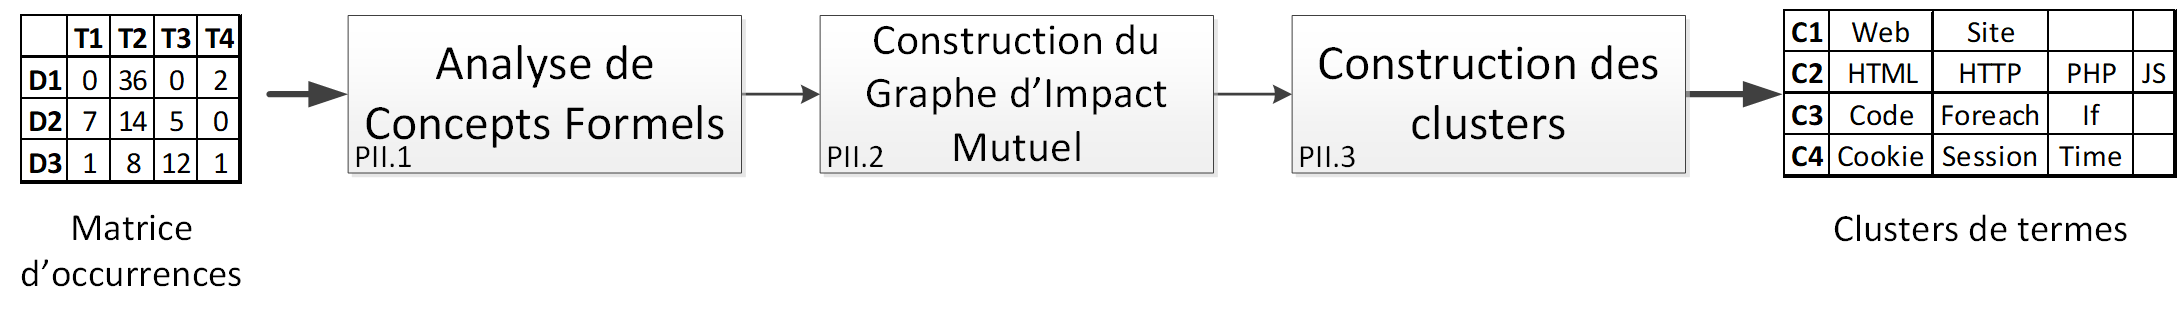
\includegraphics[scale=0.6]{3-Methode-CREA/images/schema_analyse_structurelle.png}
\centerline{  % FORCE FIGURE OUTSIDE THE MARGIN !!! BUT STILL CENTERING !!!
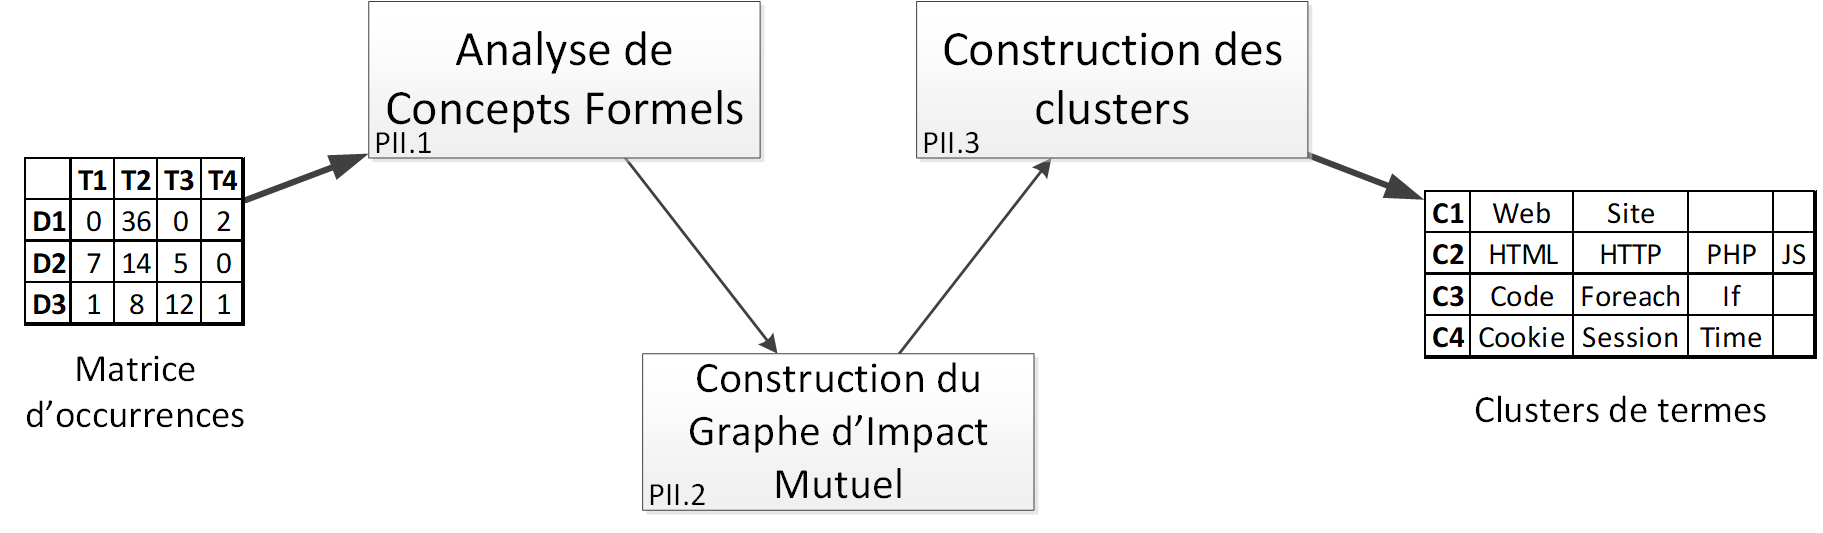
\includegraphics[scale=0.6]{3-Methode-CREA/images/schema_analyse_structurelle_ESCALIER.png}
}
\caption{Les étapes de la phase d'analyse structurelle}
\label{figure:3-II-AnalyseStructurelle}
\end{figure}
%\end{figure*} % Figure flottante
% To use it : fig~\ref{label}

\begin{itemize}
\item Analyse de Concepts Formels (PII.1) : Les techniques d'analyse de concepts formels servent à analyser les liens entre les termes et les documents les contenant afin de calculer deux métriques (l'impact mutuel et la similarité conceptuelle). Ces métriques nous permettent d'évaluer la pertinence des documents entre eux à partir des termes les plus fréquents, mais aussi d'établir la similarité des termes entre eux.
\item Construction du Graphe d'Impact Mutuel (PII.2) : L'impact mutuel entre les termes et les documents est représenté graphiquement afin de mesurer la pertinence des documents entre eux tout en affichant un ensemble de termes explicitant les principaux sujets abordés dans ces documents. Cette métrique permet d'indiquer quels documents devraient être retirés pour obtenir les meilleurs regroupements de termes.
\item Construction des clusters (PII.3) : À partir de la similarité conceptuelle des termes entre eux, des clusters de termes sont formés pour présenter à l'utilisateur les fragments réutilisables pour le cas traité.
\end{itemize}


\subsection{Analyse de Concepts Formels (PII.1)}
\label{subsection:CREA:PII.1-ACF}

L'Analyse de Concepts Formels, présentée en sous-section~\ref{subsection:Contexte:TechniquesUtilisees:ACF}, est un ensemble de techniques permettant de \og \textit{découvrir et [de] structurer des connaissances} \fg~\cite{jaffal2019aide} à partir d'une matrice rassemblant des \textit{objets} et leurs \textit{attributs}.
Appliquée au domaine de l'enseignement, avec une matrice de supports de cours et de termes les composant, il s'agit de rechercher les relations entre ces termes et les supports de cours afin d'en extraire des métriques de similarité conceptuelle et d'impact mutuel.
Ces métriques permettent ensuite d'obtenir une vision globale de l'ensemble du corpus documentaire, et d'en déduire les sujets centraux à partir des termes, mais également la pertinence des supports de cours par rapport à ces sujets centraux.
Le principe général de l'ACF se déroule en plusieurs sous-étapes illustrées par la figure~\ref{figure:3-II-1-ACF-Details}.

%\begin{figure*} % Figure flottante
\begin{figure}[ht]
\centering
%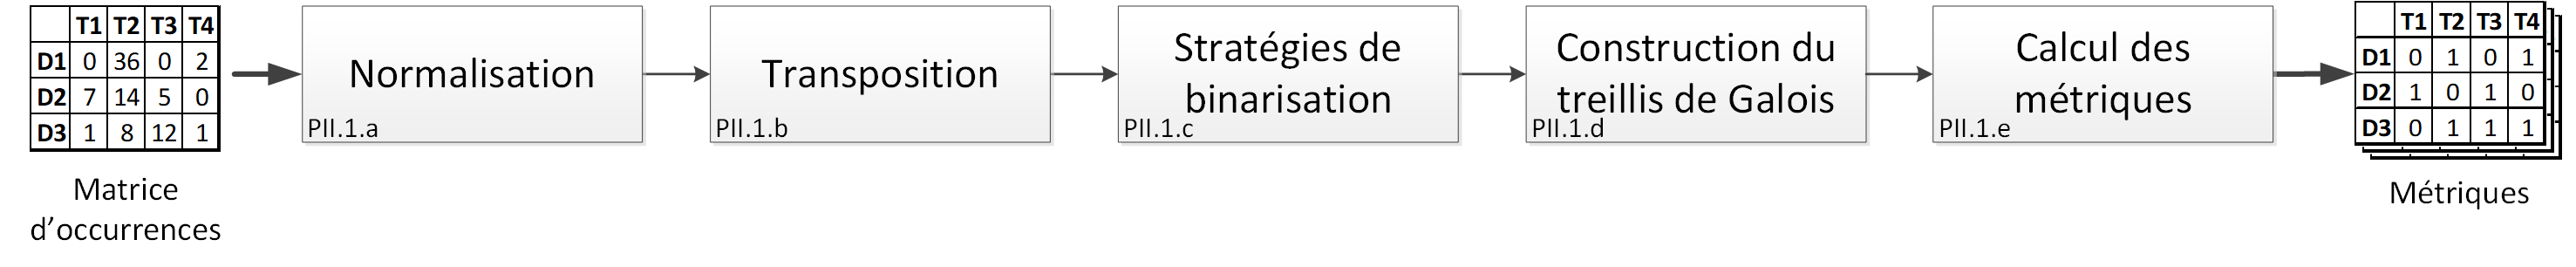
\includegraphics[scale=0.49]{3-Methode-CREA/images/schema_analyse_structurelle-ACF.png}
\centerline{  % FORCE FIGURE OUTSIDE THE MARGIN !!! BUT STILL CENTERING !!!
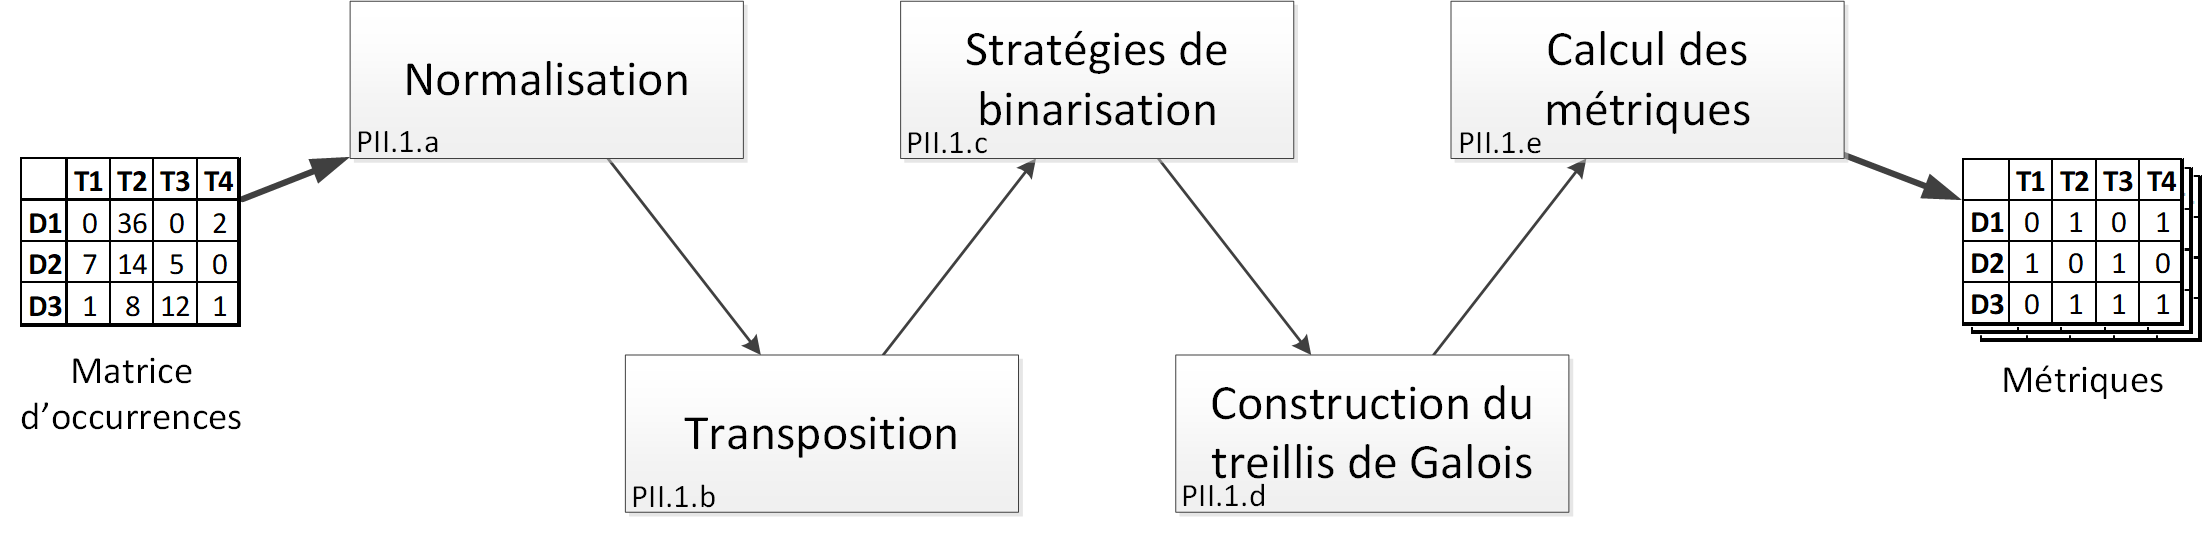
\includegraphics[scale=0.55]{3-Methode-CREA/images/schema_analyse_structurelle-ACF_ESCALIER.png}
}
\caption{Les sous-étapes de l'analyse de concepts formels}
\label{figure:3-II-1-ACF-Details}
\end{figure}
%\end{figure*} % Figure flottante
% To use it : fig~\ref{label}


\subsubsection{Normalisation (PII.1.a) :}
\label{subsubsection:CREA:PII.1.a-normalisation}

Afin de binariser la matrice d'occurrences pour en faire un \textit{contexte formel}  nous avons choisi de prendre en compte la taille des documents.
Un document contenant des milliers de termes au milieu de documents contenant une centaine de termes chacun créera une disproportion.
Afin de limiter l'effet de ce biais, une première étape vise à normaliser les quantités proportionnellement à la taille des documents : les occurrences des termes sont transformées en proportions d'occurrences dans chacun des documents.
La figure~\ref{figure:3-II-1-a-Normalisation} illustre l'étape de normalisation.

%\begin{figure*} % Figure flottante
\begin{figure}[ht]
\centering
%\includegraphics[width=3in]{images/VerySmallModels_text.png}
%%\includegraphics[scale=0.6]{images/VerySmallModels_text.png}
\centerline{  % FORCE FIGURE OUTSIDE THE MARGIN !!! BUT STILL CENTERING !!!
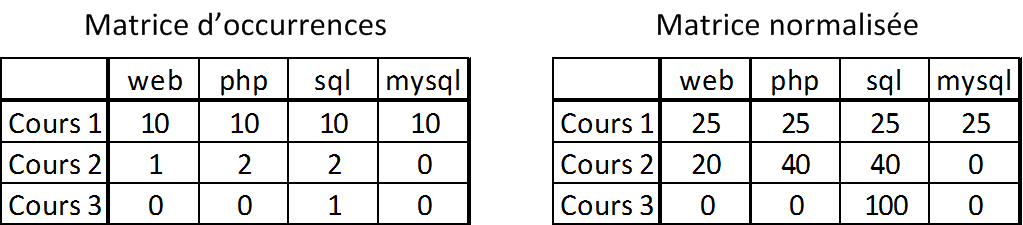
\includegraphics[scale=1]{3-Methode-CREA/images/2-analyse-structurelle/exemple_normalisation.png}
}
\caption{Exemple de normalisation d'une matrice d'occurrences}
\label{figure:3-II-1-a-Normalisation}
\end{figure}
%\end{figure*} % Figure flottante
% To use it : fig~\ref{label}

%
%XX;T1;T2;T3;T4
%C1;01;00;42;01
%C2;10;10;10;10
%C3;01;02;02;00
%C4;00;00;01;00
%
%XX;T1;T2;T3;T4
%C1;03;00;96;03
%C2;25;25;25;25
%C3;20;40;40;00
%C4;00;00;100;0
%


\subsubsection{Transposition (PII.1.b) :}
\label{subsubsection:CREA:PII.1.b-transposition}

Le sens de lecture des lignes et colonnes de la matrice est important pour les stratégies de binarisation, l'ACF, et l'interprétation des fragments qui en seront extraits.
L'ACF construisant un treillis avec des \textit{objets} caractérisés par des \textit{attributs} issus d'un \textit{contexte formel} (une matrice binaire), et les stratégies se basant sur ces caractéristiques pour générer ce \textit{contexte formel}, il est important que la matrice d'entrée soit correctement présentée : les \textit{objets} forment les lignes, et les \textit{attributs} forment les colonnes.
En l'état, les documents (objets) sont caractérisés par les termes (attributs) les composant.
Afin de changer de point de vue, et mettre en avant les connaissances réutilisables, c'est-à-dire les liens entre termes et documents, il est nécessaire de transposer la matrice pour permettre de caractériser les termes (objets) selon les documents (attributs) dans lesquels ils apparaissent.
La figure~\ref{figure:3-II-1-b-Transposition} illustre l'étape de transposition.

%\begin{figure*} % Figure flottante
\begin{figure}[ht]
\centering
%\includegraphics[width=3in]{images/VerySmallModels_text.png}
%%\includegraphics[scale=0.6]{images/VerySmallModels_text.png}
\centerline{  % FORCE FIGURE OUTSIDE THE MARGIN !!! BUT STILL CENTERING !!!
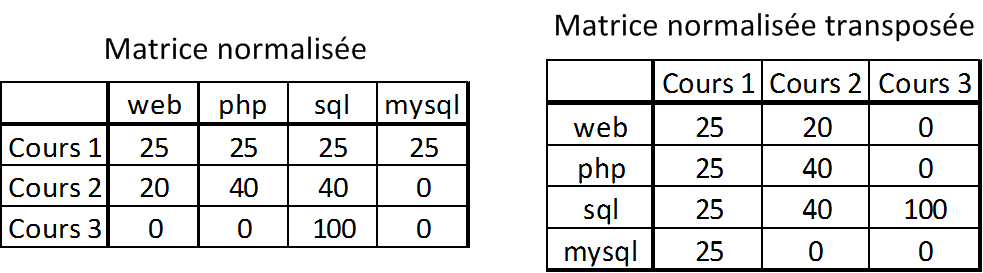
\includegraphics[scale=1]{3-Methode-CREA/images/2-analyse-structurelle/exemple_transposition.png}
}
\caption{Exemple de transposition pour caractériser les termes selon les documents où ils apparaissent}
\label{figure:3-II-1-b-Transposition}
\end{figure}
%\end{figure*} % Figure flottante
% To use it : fig~\ref{label}


\subsubsection{Stratégies de binarisation (PII.1.c) :}
\label{subsubsection:CREA:PII.1.c-strategies}

La matrice d'occurrences étant normalisée et transposée pour mettre en avant les termes caractérisés par les documents dans lesquels ils apparaissent, il est maintenant possible d'appliquer une stratégie permettant de transformer les occurrences en valeurs binaires pour obtenir un \textit{contexte formel} nécessaire à la construction du treillis dans les étapes suivantes.
Une stratégie de binarisation définit un algorithme qui transforme les valeurs d'une matrice de l'intervalle $ [ 0, +\infty [ $ vers la paire $ \{ 0, 1 \} $.

\bigskip

Il existe actuellement plusieurs stratégies~\cite{jaffal2015refinement}\cite{jaffal2019aide} pour permettre à l'ACF de présenter différentes informations contenues dans une matrice multivaluée.
Ces stratégies sont présentées en sous-section~\ref{subsubsection:Contexte:ACF-StrategiesBinarisation}.
Les métriques visées par la méthode CREA impliquent de générer les contextes formels de plusieurs de ces stratégies.
La stratégie \textit{directe} permet d'avoir une vision d'ensemble du corpus utile pour évaluer l'ensemble des sujets centraux et la pertinence des documents entre eux (les valeurs non-nulles sont remplacées par des 1, et les valeurs nulles sont remplacées par des 0).
La stratégie \textit{haute} utilisant un $ \beta = 1.00 $ permet de ne retenir que les termes dont les valeurs de fréquences d'apparition dans les documents sont les plus hautes.
Cette stratégie permet de retenir les termes les plus fréquents pour l'ensemble du corpus, mais également pour certains ensemble de documents.

\bigskip

La figure~\ref{figure:3-II-1-c-Strategies-Exemple-Directe-Haute} illustre ces deux stratégies (Directe et Haute avec un $ \beta $ fixé à 1,00).
On remarque que les valeurs non nulles de chaque ligne sont distribuées différemment entre les deux stratégies : \textit{sql} apparaissant dans tous les cours de façon non négligeable à chaque fois, c'est-à-dire que tous les cours parlent de \textit{sql} et l'un lui est dédié, il est le seul terme à être conservé sur la stratégie haute.
Cet exemple, plutôt extrême, sert à bien distinguer les objectifs différents des deux stratégies : la stratégie directe permet de voir que le cours \textit{C3} ne dispose que d'une seule notion, et devrait donc être retiré du corpus, à l'inverse, la stratégie haute récupère en effet le sujet central de \textbf{l'ensemble} du corpus documentaire, qui est \textit{sql}.
Un enseignant doit donc s'assurer tout d'abord avec la stratégie directe que les documents insérés sont cohérents, puis, une fois les documents correctement sélectionnés, il peut appliquer la stratégie haute pour en extraire les notions essentielles.


%\begin{figure*} % Figure flottante
\begin{figure}[ht]
\centering
%\includegraphics[width=3in]{images/VerySmallModels_text.png}
%%\includegraphics[scale=0.6]{images/VerySmallModels_text.png}
\centerline{  % FORCE FIGURE OUTSIDE THE MARGIN !!! BUT STILL CENTERING !!!
\includegraphics[scale=1]{3-Methode-CREA/images/2-analyse-structurelle/exemple_strategies_directe_haute_beta=1.00.png}
}
\caption{Exemple d'application des stratégies directe et haute avec un $ \beta = 1,00 $}
\label{figure:3-II-1-c-Strategies-Exemple-Directe-Haute}
\end{figure}
%\end{figure*} % Figure flottante
% To use it : fig~\ref{label}



\subsubsection{Construction du treillis de Galois (PII.1.d) :}
\label{subsubsection:CREA:PII.1.d-treillis}

Le \textit{contexte formel} généré avec les stratégies de binarisation contient maintenant des termes liés à des documents par des $ 0 $ et des $ 1 $.
Il peut donc être transformé en un \textit{treillis de Galois} composé de \textit{concepts formels} qui serviront à produire l'impact mutuel et la similarité conceptuelle.
Le \textit{treillis} est un graphe dont chaque n\oe{}ud correspond à un \textit{concept formel}.
Chaque \textit{concept formel} rassemble des \textit{objets} et leurs \textit{attributs} (et inversement, des \textit{attributs} et les \textit{objets} auxquels ils sont rattachés).
Dans notre cas, il s'agit donc de créer des concepts formels contenant des termes et les documents où ils apparaissent.
La construction d'un treillis est présentée plus en détails en sous-section~\ref{subsubsection:Contexte:ACF-ConstructionTreillis}.

Nous avons utilisé la bibliothèque \textit{Concepts}\footnote{ \href{https://concepts.readthedocs.io/en/stable/}{Page du projet \textit{Concepts} pour Python} } en Python pour automatiser la construction des treillis à partir des matrices précédentes.


\subsubsection{Calcul des métriques du treillis (PII.1.e) :}
\label{subsubsection:CREA:PII.1.e-metriquestreillis}

L'ACF permet de calculer l'impact mutuel et la similarité conceptuelle sur le treillis généré~\cite{jaffal2019aide}.
Ces métriques sont présentées en sous-section~\ref{subsubsection:Contexte:ACF-MetriquesTreillis}.
Dans le cas de la méthode CREA, nous nous concentrons particulièrement sur l'impact mutuel, qui permet de générer des graphiques utiles pour l'amélioration de la qualité des données, et la similarité conceptuelle permettant la construction des clusters de termes.


\paragraph{Similarité Conceptuelle entre objets :}
\label{mystep:CREA:PII.1.e-metrique-similariteobjets}

La \textit{similarité conceptuelle} permet de comparer deux objets (respectivement attributs) en tenant compte de leur présence dans l'ensemble du treillis.
C'est-à-dire, est-ce que les deux objets apparaissent souvent ensemble dans les concepts formels ?
Pour un enseignant, cette métrique permet de retrouver quelles notions sont les plus similaires entre elles pour les regrouper.
Techniquement, dans le cadre de la méthode CREA, la matrice de similarité conceptuelle permet d'établir la similarité entre l'ensemble des termes afin de pouvoir créer des clusters.
Suite à nos expérimentations (présentées dans la sous-section~\ref{subsubsection:Evaluation:ProtocoleEvaluation:ValidationsStructurellesFonctionnellesREX:Structurelle}), nous avons fixé les paramètres de cette métrique en utilisant le treillis représentant la matrice de stratégie haute avec un $ \beta = 1.00 $ .
En effet, nous avons empiriquement constaté que la stratégie haute permet d'obtenir les termes les plus représentatifs de l'ensemble des documents, donc d'établir une vue globale des notions abordées, et $ \beta = 1.00 $ filtre suffisamment les termes pour obtenir les meilleurs résultats.



\paragraph{Impact mutuel entre un objet et un attribut :}
\label{mystep:CREA:PII.1.e-metrique-impactmutuel}

L'\textit{impact mutuel} analyse la "\textit{force de la relation entre un objet et un attribut en fonction des concepts formels qui les associent}"~\cite{jaffal2019aide}.
Cette métrique permet de visualiser quels documents partagent le plus de notions, et réciproquement, quelles notions sont les plus présentes dans les documents.
Pour un enseignant, il s'agit d'identifier les notions clés de l'ensemble du corpus documentaire, mais aussi quels documents sont les moins représentatifs (afin de les retirer).
En assemblant les mesures d'impact mutuel entre tous les objets et attributs, une \textit{matrice d'impact mutuel} est formée.
Cette matrice d'impact mutuel permet de générer un \textit{graphe d'impact mutuel} dans l'étape suivante.
Afin d'avoir une vision d'ensemble, elle est générée à partir du treillis représentant la matrice de stratégie directe.


\subsection{Construction du Graphe d'Impact Mutuel (PII.2)}
\label{subsection:CREA:PII.2-GrapheImpactMutuel}

La \textit{Construction du Graphe d'Impact Mutuel} permet de visualiser la matrice d'impact mutuel et en déduire plusieurs informations importantes pour l'utilisateur.
Le graphe d'impact mutuel a la particularité d'être bi-parti, en proposant des n\oe{}uds de la classe des objets, et des n\oe{}uds de la classe des attributs.
Dans la méthode CREA, il s'agit donc de n\oe{}uds représentant des termes et des documents.

\bigskip

Une communauté de termes qui apparaissent visuellement au centre du graphe permet d'identifier clairement les termes les plus employés dans l'ensemble du corpus.
Cet ensemble central est déduit du degré de connexion des n\oe{}uds de la classe des termes : plus le n\oe{}ud d'un terme est connecté à des n\oe{}uds de cours, plus il est situé au centre (et réciproquement, moins il est connecté, plus il est éloigné).
À partir de cette visualisation, il est possible de comprendre quels sujets sont abordés par l'ensemble des documents, ou au contraire par certains documents précis.
La visualisation permet également de voir si quelques documents sont complètement ou partiellement hors sujet : les documents hors sujet étant peu reliés aux termes apparaissant dans l'ensemble central, leurs n\oe{}uds sont particulièrement excentrés.

\bigskip

Pour notre usage, l'utilisateur peut donc déduire si le corpus documentaire correspond à ses attentes selon les notions abordées (via les termes au centre), et éventuellement si certains documents devraient être retirés dans le cas où ceux-ci sont partiellement ou complètement hors sujet.

\bigskip

Lors de nos expérimentations, nous avons utilisé le logiciel \textit{Gephi}~\cite{bastian2009gephi} pour visualiser les matrices d'impact mutuel sous forme de graphe.
Précisément, nous avons utilisé la spatialisation \textit{Force Atlas} qui est un algorithme basé sur les forces~\cite{venturini2021we} (\og \textit{force-based} \fg ou encore \og \textit{force-directed} \fg en anglais).

La \textit{visualisation} cherche à projeter sur un plan des graphiques de points et de lignes~\cite{venturini2021we} (\og \textit{points-and-lines charts} \fg en anglais).
La \textit{spatialisation} est une forme de visualisation qui s'intéresse particulièrement à l'espace créé par la projection des données : l'espace de sortie n'est plus considéré comme une contrainte (réduisant le nombre de dimensions), mais bien comme une donnée de sortie liée aux objets projetés.
Les algorithmes basés sur les forces permettent de placer les n\oe{}uds d'un graphe en respectant un principe : les n\oe{}euds se repoussent mutuellement avec une \textit{force de répulsion}, et les arcs attirent les n\oe{}uds avec une \textit{force d'attraction}~\cite{venturini2021we}.
Ces algorithmes tendent à espacer les n\oe{}uds faiblement liés, et au contraire, à rapprocher les n\oe{}uds fortement liés~\cite{venturini2021we}.
L'algorithme \textit{Force Atlas} est une spatialisation propre à Gephi dont l'objectif est de \og \textit{permettre une interprétation rigoureuse des graphes [...] le plus directement et lisiblement possible malgré un temps d'exécution assez long} \fg~\cite{gephi2016spatialisationFR}.
Il peut s'appliquer sur des graphes comptant de $ 1 $ à $ 10000 $ n\oe{}uds avec une complexité en $ O(N^2) $~\cite{gephi2011tutoriallayout}\cite{gephi2016spatialisationFR}.
\textit{Force Atlas} permet à l'utilisateur de sélectionner plusieurs paramètres tels que les forces d'attraction, de répulsion, et quelques autres afin de placer les n\oe{}uds~\cite{jacomy2014forceatlas2}.
%
% Sources de Force Atlas :
% https://github.com/gephi/gephi/blob/db454c59cc9da3f47b7268de4ccbfa73b7f5245e/modules/LayoutPlugin/src/main/java/org/gephi/layout/plugin/forceAtlas/ForceAtlasLayout.java#L64
%


La figure~\ref{figure:3-II-2-Graphe-zoom} illustre le graphe d'impact mutuel entre des termes et des documents.
Sur la gauche, le graphe dans son ensemble est affiché.
Sur la droite, un zoom est effectué sur les termes apparaissant au c\oe{}ur du graphe.
Les n\oe{}uds en rouge sont les termes connectés à tous les cours, les n\oe{}uds en orange sont connectés à tous les cours sauf 1, les n\oe{}uds en jaune sont connectés à tous les cours sauf 2, et ainsi de suite.
Les n\oe{}uds gris représentent les supports de cours.
En lisant ce graphe, on peut voir que les termes qui apparaissent au c\oe{}ur du graphe sont \textit{post}, \textit{méthode post}, \textit{nombre}, \textit{langage}, \textit{donnée}, \textit{fichier}, \textit{code}, \textit{php}, \textit{navigateur}, \textit{site}.
La combinaison de certains termes permet de comprendre assez vite qu'il s'agit de cours sur du développement web, en particulier de PHP.


La figure~\ref{figure:3-II-2-Graphe-cours} illustre cette fois la distance entre les documents.
Typiquement, le cours \textit{C6} semble très éloigné de l'ensemble, tout comme le cours \textit{C3}, et légèrement \textit{C5}.
Il apparait donc judicieux de se pencher plus en détails sur ces derniers pour vérifier leur pertinence pour le corpus documentaire rassemblé.



Au delà du manque de pertinence d'un document par rapport aux termes, un utilisateur peut également décider d'écarter un document si certains termes contenus ne devraient pas apparaître dans les clusters finaux.
À l'issue de cette étape, l'utilisateur peut donc décider de supprimer certains documents et ré-exécuter l'analyse de concepts formels à partir de la matrice épurée des documents en question, ou de continuer avec les données déjà générées.


% esthétique
\newpage

%\vfill
%\hspace{0pt}

\begin{figure}[ht!]
\centering
\centerline{  % FORCE FIGURE OUTSIDE THE MARGIN !!! BUT STILL CENTERING !!!
\includegraphics[scale=0.6]{3-Methode-CREA/images/2-analyse-structurelle/exemple_graphe.png}
}
\caption{Graphe d'impact mutuel (généré avec Gephi en utilisant la spatialisation \textit{Force Atlas} et la coloration par \textit{partition} selon le \textit{degré})}
\label{figure:3-II-2-Graphe-zoom}
\end{figure}


\begin{figure}[ht!]
\centering
\centerline{  % FORCE FIGURE OUTSIDE THE MARGIN !!! BUT STILL CENTERING !!!
%\includegraphics[scale=0.2]{3-Methode-CREA/images/2-analyse-structurelle/exemple_graphe_large_cours.png}
% 0.7
\includegraphics[scale=0.78]{3-Methode-CREA/images/2-analyse-structurelle/exemple_graphe_large_cours.png}
}
\caption{Graphe d'impact mutuel (généré avec Gephi en utilisant la spatialisation \textit{Force Atlas} et la coloration par \textit{partition} selon le \textit{degré})}
\label{figure:3-II-2-Graphe-cours}
\end{figure}


%\hspace{0pt}
%\vfill

% esthétique
\clearpage

\subsection{Construction des clusters (PII.3)}
\label{subsection:CREA:PII.3-ConstructionClusters}

La \textit{construction des clusters} est l'ultime étape construisant des clusters à partir de la matrice de similarité conceptuelle des termes.
Ces clusters correspondent aux fragments réutilisables, c'est-à-dire dans le contexte de l'enseignement, les notions à aborder ensemble et pouvant former un syllabus.
Plusieurs techniques de clustering sont présentées en sous-section~\ref{subsection:Contexte:TechniquesUtilisees:Clustering}.
Selon l'implémentation employée, il est parfois nécessaire de transformer la matrice de similarité en une \textit{matrice de dissimilarité}.

\bigskip

Dans nos travaux, nous avons opté pour la \textit{classification ascendante hiérarchique} (ou CAH) afin d'obtenir des clusters non-recouvrants permettant de ne placer chaque terme que dans un seul cluster, tout en indiquant le nombre de clusters que l'utilisateur souhaite.
En pratique, l'implémentation de CAH inclue dans la bibliothèque SciPy~\cite{2020SciPy-NMeth} en Python exige une matrice de distance ou à minima une matrice avec la dissimilarité entre chacun des objets.
Ainsi, pour transformer notre matrice de similarité en matrice de dissimilarité (composée de valeurs entre $ 0 $ et $ 1 $), nous avons utilisé la méthode la plus simple présentée dans~\cite{rakotomalala2020pratique} consistant à soustraire chaque valeur de similarité à la valeur de similarité maximale, c'est-à-dire soustraire chacune des valeurs à $ 1 $ (les $ 1 $ devenant des $ 0 $, et ainsi de suite jusqu'aux $ 0 $ devenant des $ 1 $).
La formule~\eqref{equation:3-Calcul-Dissimilarite} illustre ce calcul.

\begin{equation}
\text{\textit{dissimilarité}}(\text{\textit{objet A}}, \text{\textit{objet B}}) = 1 - \text{\textit{similarité}}(\text{\textit{objet A}}, \text{\textit{objet B}})
\label{equation:3-Calcul-Dissimilarite}
\end{equation}


\bigskip

Afin d'appliquer la CAH, nous avons utilisé les bibliothèques scikit-learn~\cite{scikit-learn} et SciPy~\cite{2020SciPy-NMeth}.
Précisément, nous avons appliqué trois traitements successifs afin de générer les clusters finaux.
\begin{enumerate}
\item Nous standardisons tout d'abord les valeurs grâce à \textit{sklearn.preprocessing.scale()} en laissant les paramètres par défaut.
\item Nous appliquons ensuite le traitement effectuant l'agglomération des clusters individuels avec \textit{scipy.cluster.hierarchy.linkage()}.
Nous demandons l'usage de la méthode de Ward (\texttt{\textit{method='ward'}}) avec une métrique euclidienne pour ce traitement. (\texttt{\textit{metric='euclidean'}})
\item Nous utilisons enfin \textit{scipy.cluster.hierarchy.fcluster()} pour récupérer la liste des clusters.
Nous demandons de rechercher un maximum de clusters possibles \\ (\texttt{\textit{criterion='maxclust'}}) en visant 8 clusters (\texttt{\textit{t=8}}).
\end{enumerate}

\bigskip

La figure~\ref{figure:3-II-3-Clusters} illustre un résultat en huit clusters, c'est-à-dire pour huit séances.
Les clusters n'étant pas ordonnés, c'est à l'enseignant que revient ce choix.
Une technique d'ordonnancement temporelle, encore en cours d'évaluation, est proposée en sous-section~\ref{subsection:Conclusion:PerspectivesAmeliorations:AnalyseTemporelle}.

\bigskip

Dans tous les cas, ces clusters constituent une base réutilisable de termes dont l'utilisateur peut se servir pour traiter son nouveau cas.


\bigskip

\vfill
\hspace{0pt}

%\begin{figure*} % Figure flottante
\begin{figure}[ht]
\centering
\centerline{  % FORCE FIGURE OUTSIDE THE MARGIN !!! BUT STILL CENTERING !!!
% 0.65
\includegraphics[scale=0.68]{3-Methode-CREA/exemples/clusters/clusters.png}
}
\caption{Liste de huit clusters générés}
\label{figure:3-II-3-Clusters}
\end{figure}
%\end{figure*} % Figure flottante
% To use it : fig~\ref{label}


\hspace{0pt}
\vfill



%%%%%%%%%%%%%%%%%%%%%%%%%%%%%%%%%%%%%%%%%%%%%%%%%%%%%%%%%%%%%%%%%%%%%%%%%%%%%%%%%%%%%%%%%%
%%%%%%%%%%%%%%%%%%%%%%%%%%%%%%%%%%%%%%%%%%%%%%%%%%%%%%%%%%%%%%%%%%%%%%%%%%%%%%%%%%%%%%%%%%
%%%%%%%%%%%%%%%%%%%%%%%%%%%%%%%%%%%%%%%%%%%%%%%%%%%%%%%%%%%%%%%%%%%%%%%%%%%%%%%%%%%%%%%%%%
%%%%%%%%%%%%%%%%%%%%%%%%%%%%%%%%%%%%%%%%%%%%%%%%%%%%%%%%%%%%%%%%%%%%%%%%%%%%%%%%%%%%%%%%%%
%%%%%%%%%%%%%%%%%%%%%%%%%%%%%%%%%%%%%%%%%%%%%%%%%%%%%%%%%%%%%%%%%%%%%%%%%%%%%%%%%%%%%%%%%%
%%%%%%%%%%%%%%%%%%%%%%%%%%%%%%%%%%%%%%%%%%%%%%%%%%%%%%%%%%%%%%%%%%%%%%%%%%%%%%%%%%%%%%%%%%
%
%\newpage
%
%%%%%%%%%%%%%%%%%%%%%%%%%%%%%%%%%%%%%%%%%%%%%%%%%%%%%%%%%%%%%%%%%%%%%%%%%%%%%%%%%%%%%%%%%%
%%%%%%%%%%%%%%%%%%%%%%%%%%%%%%%%%%%%%%%%%%%%%%%%%%%%%%%%%%%%%%%%%%%%%%%%%%%%%%%%%%%%%%%%%%
%%%%%%%%%%%%%%%%%%%%%%%%%%%%%%%%%%%%%%%%%%%%%%%%%%%%%%%%%%%%%%%%%%%%%%%%%%%%%%%%%%%%%%%%%%
%%%%%%%%%%%%%%%%%%%%%%%%%%%%%%%%%%%%%%%%%%%%%%%%%%%%%%%%%%%%%%%%%%%%%%%%%%%%%%%%%%%%%%%%%%
%%%%%%%%%%%%%%%%%%%%%%%%%%%%%%%%%%%%%%%%%%%%%%%%%%%%%%%%%%%%%%%%%%%%%%%%%%%%%%%%%%%%%%%%%%
%%%%%%%%%%%%%%%%%%%%%%%%%%%%%%%%%%%%%%%%%%%%%%%%%%%%%%%%%%%%%%%%%%%%%%%%%%%%%%%%%%%%%%%%%%


%%%%%%%%%%%%%%%%%%%%%%%%%%%%%%%%%%%%%%%
%\section{Analyse temporelle : organisation des scénarios}% :
%\label{section:CREA:PIII-AnalyseTemporelle}
%
%
%\subsection{Découpage des documents en sections (PIII.1)}
%\label{subsection:CREA:PIII.1-DecoupageDocuments}
%
%\subsection{Sélection des étiquettes temporelles (PIII.2)}
%\label{subsection:CREA:PIII.2-SelectionEtiquettesTemporelles}
%
%\subsection{Étiquetage temporel des clusters (PIII.3)}
%\label{subsection:CREA:PIII.3-EtiquetageTemporelClusters}
%
%\subsection{Organisation en séances (PIII.4)}
%\label{subsection:CREA:PIII.4-OrganisationSeances}


%------------------------------------------------

% Expériences et Evaluations de la méthode (Méthodologie de Recherche + Données + Evaluations)
% "Expériences / Evaluations"
% \'Evaluations
\chapter{Évaluation et Validation de la méthode CREA}
\label{chapter:Evaluation}

Dans ce chapitre, nous évaluons la méthode CREA décrite précédemment et discutons ces résultats.
Les expérimentations sont effectuées selon la démarche méthodologique de \textit{design science}~\cite{hevner2004design}\cite{hevner2007three} décrite par la suite.
Nous présentons un protocole d'évaluation basé sur plusieurs validations (structurelles, fonctionnelles, et par retour d'expérience), puis nous l'exécutons.
Enfin, nous discutons des conclusions de ces expérimentations, des limites de la méthode CREA, et de la méthodologie d'évaluation en elle-même.


\bigskip

\minitoc % Creating an actual minitoc / ToC local to a chapter

\newpage

%%%%%%%%%%%%%%%%%%%%%%%%%%%%%%%%%%%%%%%%%%%%%%%%%%%%%%%%%

\section{Méthodologie d'évaluation}
\label{section:Evaluation:MethodologieEvaluation}

La \textit{science du design}~\cite{hevner2004design}\cite{hevner2007three}\cite{peffers2007design}\cite{pascal2011approche}, ou \textit{design science} en anglais, décrit une méthodologie de recherche permettant de développer et évaluer un artefact visant à répondre à une question de recherche.
Cette méthodologie de recherche appliquée au système d'informations s'appuie sur trois boucles d'activités (pertinence, rigueur, et design) décrites dans~\cite{hevner2007three} et \cite{pascal2011approche}, et illustrées par la figure~\ref{figure:1-S3-DesignScience-ThreeLoops}.
Chaque boucle décrit un ensemble d'activités à réaliser successivement pour produire un artefact de meilleure qualité à chaque itération :
\begin{itemize}
\item La \textit{boucle de pertinence} permet de déterminer les problèmes ou opportunités d'un domaine d'étude en particulier, et les critères nécessaires à évaluer (dans le cadre de recherche plus général~\cite{hevner2004design}, il s'agit des critères permettant de valider les tests fonctionnels).
Cette boucle est itérée autant de fois que nécessaire tant que les critères fonctionnels ne sont pas validés.

\item La \textit{boucle de rigueur} permet de choisir les théories et méthodes les plus adaptées~\cite{pascal2011approche} pour répondre à la question de recherche, et donc déterminer les solutions déjà proposées dans le domaine de recherche.
Cette boucle permet de construire et alimenter une base de connaissances, elle se rapproche d'une revue de la littérature ou d'un état de l'art.

\item La \textit{boucle de design} s'appuie sur deux activités en particulier : la conception et l'évaluation~\cite{pascal2011approche}.
Ces activités dépendent des résultats des deux autres boucles afin de déterminer quoi réaliser (par rapport aux exigences), quels résultats sont visés (par rapport aux critères de validation), et enfin qu'est-ce que ces travaux apportent à la base de connaissances.
\end{itemize}

\bigskip

%\begin{figure*} % Figure flottante
\begin{figure}[ht]
\centering
\centerline{  % FORCE FIGURE OUTSIDE THE MARGIN !!! BUT STILL CENTERING !!!
% scale = 0.7    0.68 (sans enumerate)
\includegraphics[scale=0.78]{1-Introduction/images/MethodeRecherche/Cycles-Design-Science.png}
}
\caption{Les trois boucles de la science du design présentées dans~\cite{hevner2007three} et \cite{pascal2011approche}}
\label{figure:1-S3-DesignScience-ThreeLoops}
\end{figure}
%\end{figure*} % Figure flottante
% To use it : fig~\ref{label}

\bigskip
%\vspace*{1pt}

Pour répondre à notre question de recherche, nous avons effectué une méthodologie de recherche s'inspirant particulièrement de la science du design.
Tout d'abord, nous avons réalisé une étude du domaine des processus à forte intensité des connaissances et l'avons publié dans un article~\cite{boissier2019challenges}.
Celle-ci a permis de mettre en évidence six défis récurrents dans le domaine des processus à forte intensité de connaissances en étudiant les différents fondements théoriques et réponses actuellement apportées par la recherche.
Cette étude a donc contribué aux boucles de pertinence et de rigueur en construisant un premier cadre.
Afin d'évaluer les résultats d'une contribution pouvant relever certains des défis présentés, nous avons choisi un domaine particulièrement adapté à la manipulation de connaissances et rencontrant actuellement des difficultés suite à la crise du COVID-19 : l'enseignement supérieur et la recherche.
Notre premier objectif a été de proposer une méthode permettant d'aider à construire le cours le plus pertinent possible pour un sujet donné en s'appuyant sur la réutilisation de fragments de processus.
Notre stratégie de validation pour la méthode CREA consiste à la réalisation et l'analyse de cinq scénarios de création de cours ainsi qu'un retour d'expérience basé sur des entretiens.

\bigskip
%\vspace*{1pt}

Un premier scénario servant de cas de référence a été réalisé afin d'établir une première itération de la boucle de design et vérifier les critères attendus pour les domaines de recherche et d'application.
Ce premier scénario vise à rassembler plusieurs supports de cours traitant d'un même sujet, afin de pouvoir en extraire des fragments réutilisables (des notions à présenter à chaque séance de cours).
La boucle de design pouvant fonctionner seule, ce premier scénario nous a permis de fixer certains paramètres au sein de la méthode construite.
Ces paramètres sont présentés au fur et à mesure dans le chapitre~\ref{chapter:CREA}.
De plus, plusieurs directions ont été testées et abandonnées étant donné la faible qualité des résultats apportés.

Nous avons ensuite étendu nos objectifs en ajoutant une détection de la pertinence des supports de cours par rapport à un sujet donné.
Un deuxième scénario a donc été construit en insérant parmi les données d'entrée un document traitant d'un sujet un peu plus éloigné, mais pas complètement hors sujet.
En comparaison du premier scénario, celui-ci doit mettre en évidence que le document supplémentaire est moins pertinent que les autres, et donc qu'il n'est pas conforme.

Un troisième scénario a permis d'étudier l'impact de l'augmentation du nombre de documents sur les métriques de sorties et les clusters générés.
Deux fois plus de documents ont été insérés en entrée pour observer les effets.
Ces trois premiers cas ont surtout permis d'effectuer une validation structurelle de la méthode CREA que nous avons construite, tout en s'assurant de l'absence de problèmes fonctionnels sur le fond.

Un quatrième scénario a permis d'étudier la correction du bruit sur un support et les conséquences sur le graphe d'impact mutuel au fur et à mesure.
Certains documents précédemment utilisés ont été utilisés et l'un d'entre eux a été \textit{corrigé} en lui retirant des sections hors sujet.

Un cinquième scénario a permis d'étudier l'impact de la langue sur les clusters finaux et de la nature des documents sur leur pertinence, tout en s'assurant que la méthode n'a pas été spécialisée sur le cas de référence et ses dérivés.
Plusieurs documents de nature diversifiée en anglais (supports de cours, d'articles de recherche, et de pages web) ont été insérés en entrée.



%%%%%

Enfin, deux questionnaires ont été réalisés sur le cas de référence en interrogeant des experts du sujet traité pour s'assurer que les résultats sont exploitables par des utilisateurs.
Nous présentons dans cette thèse le résultat des multiples itérations de ces trois boucles et les cinq scénarios qui ont permis cela.

\bigskip

Cette méthodologie de recherche manipule elle-même de nombreuses connaissances et réutilise des contributions passées, ou s'en inspire grandement pour avancer plus loin.
Comme tout processus de recherche, il s'agit bien d'un processus à forte intensité de connaissances qui contribue à répondre à un problème de processus à forte intensité de connaissances (condition nécessaire).
La contribution proposée dépendant elle aussi des connaissances implicites de l'utilisateur, ainsi que des connaissances intégrées aux documents et aux bases de connaissances utilisées comme nous l'avons présenté dans les chapitres précédents, il n'y a donc pas de contradiction théorique.




%%%%%%%%%%%%%%%%%%%%%%%%%%%%%%%%%%%%%%%%%%%%
\clearpage % Clean for pictures and tables %
\newpage   % Clean for pictures and tables %
%%%%%%%%%%%%%%%%%%%%%%%%%%%%%%%%%%%%%%%%%%%%

%%%%%%%%%%%%%%%%%%%%%%%%%%%%%%%%%%%%%%%%%%%%%%%%%%%%%%%%%
%%%%%%%%%%%%%%%%%%%%%%%%%%%%%%%%%%%%%%%%%%%%%%%%%%%%%%%%%
%%%%%%%%%%%%%%%%%%%%%%%%%%%%%%%%%%%%%%%%%%%%%%%%%%%%%%%%%
%%%%%%%%%%%%%%%%%%%%%%%%%%%%%%%%%%%%%%%%%%%%%%%%%%%%%%%%%
%%%%%%%%%%%%%%%%%%%%%%%%%%%%%%%%%%%%%%%%%%%%%%%%%%%%%%%%%
%%%%%%%%%%%%%%%%%%%%%%%%%%%%%%%%%%%%%%%%%%%%%%%%%%%%%%%%%

\section{Protocole d'évaluation}
\label{section:Evaluation:ProtocoleEvaluation}


\subsection{Scénarios d'évaluation}
\label{subsection:Evaluation:ProtocoleEvaluation:ScenariosEvaluation}

Cinq scénarios ont été préparés pour pouvoir valider la méthode CREA dans plusieurs situations.
Ces scénarios visent à construire un cours en 8 séances, donc générer 8 clusters.
\begin{itemize}
\item Scénario n°1 (cas référence) : Ce scénario de référence doit pouvoir fournir des clusters de termes pertinents pour un cours de développement web en PHP.
Les clusters de termes générés doivent au moins aider un enseignant à parler des bases du développement du web avec HTML, PHP, et un peu de base de données avec MySQL.
9 supports de cours de PHP sont utilisés, 6 sont au format diapositives et 3 au format texte long.
Tous les documents fournis en entrée sont pertinents, bien qu'ils aient leurs spécificités.
Ceux-ci sont détaillés dans les paragraphes suivants afin de mieux comprendre leurs spécificités et ce qui est attendu dans le graphe d'impact mutuel.
Nous avons également réalisé une étude comparative depuis notre propre point de vue expert sur ce cas de référence.
Enfin, nous avons demandé à 5 informaticiens de construire 8 clusters à partir des termes retenus par la stratégie haute et $ \beta = 1.00 $ pour pouvoir les comparer à ceux produits par la méthode CREA.
Nous leurs avons ensuite demandé de donner leur avis sur les clusters générés par la méthode CREA.
Ainsi, ce scénario contribue à répondre aux hypothèses H1, H2, H3, H4a-b, H5, H6a-b-c, et H8a-b-c en faisant l'extraction des termes d'un premier corpus documentaire traitant d'un même sujet, puis en produisant un premier graphe d'impact mutuel et des clusters.
Ces données seront comparées à celles produites dans les autres scénarios afin de valider ou invalider les hypothèses. \\

\item Scénario n°2 : Ce scénario vise à vérifier la résistance au bruit en insérant un cours sur un sujet éloigné dans le corpus initial.
Les 9 supports de cours de PHP du scénario n°1 sont utilisés, et sont complétés d'un cours de Java au format texte long.
Le document Java traitant de développement, il sera suffisamment proche des cours de PHP pour avoir quelques liens sémantiques, mais le c\oe{}ur du sujet n'étant pas le développement web, ces liens sémantiques seront limités et il devrait apparaitre comme éloigné des autres documents.
Ce scénario se limite à la génération du graphe d'impact mutuel pour permettre à un enseignant de constater qu'un des documents insérés est trop peu pertinent par rapport aux autres, et qu'il faudrait donc le retirer.
Ce deuxième scénario contribue à répondre aux hypothèses H1, H2, H3, H7b, et H8a-b-c en faisant l'extraction des termes d'un deuxième corpus documentaire dont un document est incorrect, puis en produisant un second graphe d'impact mutuel devant faire apparaître une incohérence. \\

\item Scénario n°3 : Ce scénario vise à vérifier la robustesse de la méthode en doublant le nombre de documents par rapport au corpus initial.
18 supports de cours de PHP sont donc utilisés.
9 proviennent du scénario n°1 (6 au format diapositives et 3 au format texte long), et 9 autres sont ajoutés (5 au format diapositives et 4 au format texte long).
Ce troisième scénario contribue à répondre aux hypothèses H1, H2, H3, H4a-b, H5, H6a-b-c, et H8a-b-c en faisant l'extraction des termes d'un troisième corpus documentaire traitant d'un même sujet mais avec beaucoup plus de documents, puis en produisant un troisième graphe d'impact mutuel et des clusters. \\

\item Scénario n°4 : Ce scénario vise à vérifier que la méthode est fonctionnellement correcte en s'assurant que l'amélioration des documents en entrée produit un graphe d'impact mutuel reflétant ces améliorations.
7 supports de cours de PHP sont utilisés parmi les 18 du scénario n°3, en particulier, nous ne sélectionnons que ceux au format texte long.
L'un de ces supports étant considéré comme assez peu cohérent par rapport aux autres, nous étudions succinctement ses différences pour pouvoir le \textit{corriger} deux fois de suite en supprimant des sections hors sujet.
Afin de s'assurer de la validité des corrections, et de leurs conséquences, chaque test est également reproduit une deuxième fois en insérant le support de cours Java parmi les données d'entrée.
Ce quatrième scénario contribue à répondre aux hypothèses H1, H3, H7b, et H8a-b-c en étudiant l'évolution du graphe d'impact mutuel suite aux modifications dans le contenu des documents.

\item Scénario n°5 : Ce scénario a trois objectifs distincts.
Il vise tout d'abord à s'assurer que la méthode n'a pas été construite pour favoriser la détection de cours PHP, étant donné que le cas de référence a été utilisé pour fixer les paramètres tout au long des travaux de cette thèse.
Le second objectif est de valider que la partie traitement automatique du langage supporte d'autres langues, en particulier l'anglais.
Le troisième objectif est de confirmer que les documents pouvant être analysés ne se limitent pas à des supports de cours, mais peuvent être étendus à d'autres formats (page web, articles de recherche, livres, ...).
Nous avons donc testé la méthode CREA sur 13 documents en anglais traitant des Statecharts~\cite{harel1987statecharts}.
Afin de gérer l'anglais, les configurations de TreeTagger et BabelFy ont été adaptées.
Ce cinquième scénario contribue à répondre aux hypothèses H1, H2, H3, H4a-b, H5, H6a-b-c, H7a-c, et H8a-b-c en faisant l'extraction des termes d'un quatrième corpus documentaire beaucoup plus hétérogène traitant d'un sujet différent des précédents, puis en produisant un cinquième graphe d'impact mutuel et des clusters. \\

\end{itemize}

\bigskip


\begin{table}[htb!]
\centering
\centerline{  % FORCE FIGURE OUTSIDE THE MARGIN !!! BUT STILL CENTERING !!!
\begin{tabular}{ c   c   c   c  l  c  c  c  l  c  l  c  c  c  l  c  c  c  l  c  c  c  l  c }
\specialrule{.1em}{.05em}{.05em}
\multirow{2}{*}{} & \multirow{2}{*}{H1} & \multirow{2}{*}{H2} & \multirow{2}{*}{H3} & & \multicolumn{3}{c}{H4} & & \multirow{2}{*}{H5} & & \multicolumn{3}{c}{H6} & & \multicolumn{3}{c}{H7} & & \multicolumn{3}{c}{H8} & & \multirow{2}{*}{H9} \\
\cline{6-8} \cline{12-14} \cline{16-18} \cline{20-22}
                  &                     &                     &                     & &     a & b & c        & &                    &           & a & b & c        & &      a & b & c         & &      a & b & c        & &  \\

\specialrule{.1em}{.05em}{.05em}
%  & H1 & H2 & H3 & H4a & H4b & H4c &
% H5 & H6a & H6b & H6c & H7a & H7b & H7c &
% H8a & H8b & H8c & H9
%
% S1 : H1, H2, H3, H4a-b, H5, H6a-b-c, H8a-b-c
S1 & \textbullet & \textbullet & \textbullet & &  \textbullet & \textbullet & &  &
 \textbullet & &  \textbullet & \textbullet & \textbullet & &  & & &  &
 \textbullet & \textbullet & \textbullet & & \\
\hline
% S2 : H1, H2, H3, H7b, H8a-b-c
S2 & \textbullet & \textbullet & \textbullet & &  & & &  &
 & &   & &  & &  & \textbullet & &  &
 \textbullet & \textbullet & \textbullet & & \\
\hline
% H1, H2, H3, H4a-b, H5, H6a-b-c, H8a-b-c
S3 & \textbullet & \textbullet & \textbullet & &  \textbullet & \textbullet &  & &
 \textbullet & &  \textbullet & \textbullet & \textbullet & &  & & &  &
 \textbullet & \textbullet & \textbullet & & \\
\hline
% H1, H3, H7b, H8a-b-c
S4 & \textbullet & & \textbullet & &  & & &  &
 & &  & &  & &  & \textbullet & &  &
 \textbullet & \textbullet & \textbullet & & \\
\hline
% H1, H2, H3, H4a-b, H5, H6a-b-c, H7a-c, H8a-b-c
S5 & \textbullet & \textbullet & \textbullet & &  \textbullet & \textbullet &  & &
 \textbullet & &  \textbullet & \textbullet & \textbullet & &  \textbullet & & \textbullet &  &
 \textbullet & \textbullet & \textbullet & & \\
\specialrule{.1em}{.05em}{.05em}
\end{tabular}
}
\caption{Scénarios et hypothèses visées}
\label{table:4-Scenarios-Hypotheses}
\end{table}




\subsection{Validations structurelles, fonctionnelles, et par retour d'expérience}
\label{subsection:Evaluation:ProtocoleEvaluation:ValidationsStructurellesFonctionnellesREX}

Afin d'évaluer la méthode CREA, nous avons effectué plusieurs validations structurelles et fonctionnelles.
Nous nous assurons ainsi que chaque composant fonctionne, et que l'ensemble de la méthode CREA génère des résultats utiles pour un enseignant.


\subsubsection{Validations structurelles}
\label{subsubsection:Evaluation:ProtocoleEvaluation:ValidationsStructurellesFonctionnellesREX:Structurelle}

La validation structurelle du point de vue design science est décrite ainsi dans~\cite{hevner2004design} : \og \textit{Perform coverage testing of some metric (e.g., execution paths) in the artifact implementation} \fg , c'est-à-dire qu'elle vérifie certaines métriques dans l'artefact implémenté.
Elle est plus spécifiquement comparée au fonctionnement \og \textit{White Box} \fg dans lequel les composants d'un artefact sont connus avec précision, et sont testés un à un.

\bigskip

Pour effectuer la validation structurelle, nous comparons plusieurs valeurs par rapport aux documents d'entrée :
\begin{itemize}
\item Nous comptons le nombre de \textit{mots} (suite de caractères séparés par des espaces, de la ponctuation, ou des retours à la ligne) et de \textit{termes} (ensemble de mots formant un concept ou une entité nommée dans le réseau sémantique BabelNet lors de l'étape de désambiguïsation (PI.3)) dans chaque document, et nous les comparons au nombre de mots et termes conservés suite  aux étape de nettoyage des textes (PI.2) et  de filtrage des termes (PI.4).
Les pourcentages de mots et de termes conservés sont également indiqués.
Cette métrique permet de comparer les documents entre eux en cas de disproportions dans les quantités de mots ou de termes, et d'observer les conséquences sur les résultats intermédiaires et finaux.\\

\item Nous comptons le nombre de \textit{termes uniques} (entités nommées et concepts retrouvés dans le réseau sémantique BabelNet lors de l'étape de désambiguïsation (PI.3), sans prendre en compte les occurrences) retenus et exclus dans chaque document, et nous le comparons au nombre de termes uniques retenus et exclus suite à l'étape de filtrage des termes (PI.4).
Les pourcentages de termes uniques retenus et exclus, et le nombre de termes communs aux deux listes sont également indiqués.
Cette métrique permet de comparer les documents entre eux en cas de disproportions dans les quantités de termes uniques, et d'observer les conséquences sur les résultats intermédiaires et finaux.
Les termes communs servent également à mesurer le nombre de termes dont le contexte détecté par BabelFy ne correspond pas à celui qui serait attendu ou dont la désambiguïsation n'est pas sûre.\\

\item Nous comptons la quantité de termes uniques retenus pour les quatre stratégies de binarisation (directe, moyenne, haute, basse) appliquées avec cinq valeurs de $ \beta $ allant de $ 0.00 $ à $ 1.00 $ par pas de $ 0.25 $.
Cette métrique permet de vérifier la quantité de termes uniques retenus par les stratégies, et estimer la valeur de $ \beta $ la plus adaptée pour sélectionner les termes les plus importants/retirer les termes pouvant provoquer du bruit dans les traitements suivants.
Elle vise également à confirmer que les stratégies directe et haute conservent respectivement le plus de termes et une quantité limitée mais suffisante de termes pour les traitements suivants.\\

\item Nous comptons la quantité et les proportions de \og 0 \fg et de \og 1 \fg dans les matrices générées par les quatre stratégies de binarisation et les cinq valeurs de $ \beta $.
Cette métrique permet de s'assurer que les treillis générés ne seront ni trop vides (beaucoup trop de \og 0 \fg forment quelques concepts formels aux extrémités du treillis uniquement), ni trop pleins (beaucoup trop de \og 1 \fg forment toutes les combinaisons possibles de documents et de termes), mais feront suffisamment de liens entre les termes et les documents pour que des concepts formels intéressants soient formés (c'est-à-dire qu'il existe des concepts formels mélangeant plusieurs documents \textit{et} plusieurs termes, sans produire toutes les combinaisons possibles).\\

\item Nous analysons les clusters générés avec la stratégie haute afin de confirmer que le choix du $ \beta $ à $ 1.00 $ est adapté.
Les clusters générés sont comparés pour connaître le $ \beta $ générant les meilleurs clusters (c'est-à-dire ceux contenant le moins de bruit, et dont l'organisation est la plus correcte pour un expert).
Cette analyse est également réalisée avec la validation fonctionnelle étant donné qu'elle concerne la sortie finale.
\end{itemize}


\subsubsection{Validations fonctionnelles}
\label{subsubsection:Evaluation:ProtocoleEvaluation:ValidationsStructurellesFonctionnellesREX:Fonctionnelle}

La validation fonctionnelle du point de vue design science est décrite ainsi dans~\cite{hevner2004design} : \og \textit{Execute artifact interfaces to discover failures and identify defects} \fg , c'est-à-dire qu'elle vérifie si l'artefact présente des défaillances à l'usage.
Elle est plus spécifiquement comparée au fonctionnement \og \textit{Black Box} \fg dans lequel les composants d'un artefact sont inconnus, et seules les entrées et sorties peuvent être contrôlées.

\bigskip

Pour effectuer la validation fonctionnelle, nous analysons cette fois les données produites en sortie de la méthode pour chaque cas :
\begin{itemize}
\item Nous analysons le graphe d'impact mutuel formé grâce aux métriques du treillis avec la stratégie directe lors de l'étape calcul des métriques du treillis (PII.1.e) afin d'évaluer si la méthode détecte correctement quels documents portent sur le même sujet, et lesquels en sont éloignés.
La validation étant visuelle, nous observons donc quels documents sont suffisamment rapprochés pour former un groupe au centre du graphique, et quels documents sont au contraire éloignés du centre.\\

\item Nous analysons les clusters générés avec la stratégie haute afin de confirmer que la méthode fonctionne et produit des clusters pertinents pour la réutilisation.
Cette validation étant purement qualitative, nous nous sommes permis d'évaluer avec notre propre expertise les résultats.
Pour confirmer la pertinence des clusters, nous avons également demandé à des informaticiens leurs avis sur un cas servant de référence.
\end{itemize}



%\bigskip

\subsubsection{Validation par retour d'expérience}
\label{subsubsection:Evaluation:ProtocoleEvaluation:ValidationsStructurellesFonctionnellesREX:REX}


Nous avons également réalisé des entretiens en demandant un avis extérieur sur la qualité des clusters générés par la méthode CREA.
Pour cela, 5 informaticiens ont été interrogés avec deux questionnaires successifs (le deuxième n'étant envoyé qu'une fois le premier récupéré) à propos des résultats du scénario n°1 (les 9 supports de cours de développement web en PHP).
2 informaticiens sont novices en PHP (faible expérience en développement web avec PHP ou en administration d'un serveur web utilisant PHP).
3 informaticiens sont experts en PHP (nombreuses expériences en développement web, déploiement d'applications, et administration d'applications utilisant PHP).
Parmi les 3 experts en PHP, 2 ont une expérience dans l'enseignement de l'informatique et en particulier des langages de programmation.
L'objectif de diviser en deux questionnaires séparés est de récupérer tout d'abord l'avis individuel de chacun (en utilisant leurs connaissances tacites) sur l'organisation du cours idéal avec les termes uniques obtenus, avant de demander un avis critique sur les résultats de la méthode CREA.

\bigskip

Afin de connaître plusieurs dispositions possibles du point de vue humain, le premier questionnaire demande d'organiser les 60 termes issus du scénario n°1 en 8 clusters.
Les consignes suivantes ont été envoyées avec une feuille excel contenant l'ensemble des termes :
\begin{verbatim}
ORGANISER LES 60 TERMES EN 8 SEANCES DE COURS
				(voir onglet/feuille "Clusters" tout en bas)
CONTRAINTES :
 - au moins 1 terme par séance (une séance est représentée par un cluster)
 - chaque terme doit être au plus ET au moins dans une séance
\end{verbatim}

\bigskip

Le deuxième questionnaire présente tout d'abord les clusters du cas de référence avant de poser 4 questions.
Les 2 premières nous intéressent particulièrement pour cette expérience, les 2 autres servant pour des travaux ultérieurs sur l'axe temporel (voir sous-section~\ref{subsection:Conclusion:PerspectivesAmeliorations:AnalyseTemporelle} en conclusion).
Les questions sont posées comme suit :
\begin{enumerate}
\item Notez cette proposition de regroupements :
	\begin{itemize}
	\item[] (0) Les regroupements n'ont aucun sens pour un cours de PHP
		[aucun terme ne va avec un autre dans un même cluster pour faire un cours de PHP]

	\item[] (1) Seuls quelques regroupements ont un peu de logique
		[beaucoup de clusters contiennent des termes qui n'ont aucun lien entre eux pour faire un cours de PHP]
	\item[] (2) Les termes sont vaguement liés, ce serait très difficile d'en faire un cours de PHP
		[les clusters nécessitent tous au moins plusieurs modifications pour être utilisables pour faire un cours de PHP]
	\item[] (3) Les termes sont plutôt liés, mais il y a beaucoup trop de bruit pour pouvoir facilement construire un cours PHP
		[quelques clusters ont besoin d'être profondément modifiés pour faire un cours de PHP]

	\item[] (4) Les termes sont quasiment tous liés, il y a un peu de bruit, mais il est possible de construire un cours de PHP
		[les clusters sont majoritairement bons, quelques-uns ont besoin de quelques modifications pour faire un cours de PHP]

	\item[] (5) Les termes sont correctement liés, un cours peut directement en être produit
		[aucune modification n'est requise : un cours de PHP peut directement être produit]
	\end{itemize}

\item Expliquez votre choix :

\item À quel moment placeriez-vous chacun des clusters pour faire un cours de PHP ?
	\begin{itemize}
	\item[] Début :
	\item[] Milieu :
	\item[] Fin :
	\end{itemize}

\item Dans quel ordre très précis placeriez-vous chacun des clusters pour faire un cours ?
	(si vous avez un doute sur certain(s), indiquez si vous avez un doute entre plusieurs endroits OU si vous n'arrivez absolument pas à le placer)
	\begin{itemize}
	\item[] Ordre :
	\item[] Doute 1 : (hésitation entre plusieurs moments pour le placer)
	\item[]	Doute 2 : (aucune idée du moment où le placer)
	\end{itemize}
\end{enumerate}


\bigskip

Les réponses au premier questionnaire sont comparées avec l'indice de Rand~\cite{rand1971objective} et l'indice de Rand ajusté~\cite{hubert1985comparing} afin de déterminer les différences entre chacune des réponses.
Ces deux indices permettent de comparer deux partitions, c'est-à-dire comparer dans deux cas la façon dont des éléments ont été regroupés dans des clusters.

L'indice de Rand~\cite{rand1971objective} produit une mesure de similarité en comparant des paires de points entre chacune des deux partitions.
Cette mesure produit un résultat allant de $ 1 $ (les deux partitions ont strictement les mêmes clusters contenant exactement les mêmes points) à $ 0 $ (les deux partitions n'ont strictement aucune paire de points regroupée dans les mêmes clusters, par exemple comme expliqué dans~\cite{rand1971objective} : une première partition a tous ses points regroupés dans un unique cluster, et une deuxième partition a autant de clusters qu'il y a de points).
Pour calculer l'indice de Rand, on s'intéresse particulièrement à quatre types de paires de points dans chacune des deux partitions testées~\cite{hubert1985comparing}\cite{steinley2004properties} :
\begin{itemize}
\item \textit{a} : les paires de points appartenant dans les deux cas aux mêmes clusters (exemple figure~\ref{figure:4-RandIndex} : \textit{Terme 2} et \textit{Terme 4} sont ensemble dans les deux cas)
\item \textit{b} : les paires de points appartenant à des classes différentes dans le premier cas, et à la même classe dans le deuxième cas (exemple figure~\ref{figure:4-RandIndex} : \textit{Terme 1} et \textit{Terme 3} sont dans les clusters \textit{I} et \textit{II} dans le cas n°1, puis dans le cluster \textit{A} dans le cas n°2)
\item \textit{c} : les paires de points appartenant à la même classe dans le premier cas, et à des classes différentes dans le deuxième cas (exemple figure~\ref{figure:4-RandIndex} : \textit{Terme 1} et \textit{Terme 2} sont dans le cluster \textit{I} dans le cas n°1, puis dans les clusters \textit{A} et \textit{B} dans le cas n°2)
\item \textit{d} : les paires de points appartenant à des classes différentes dans les deux cas (exemple figure~\ref{figure:4-RandIndex} : \textit{Terme 1} et \textit{Terme 6} sont dans des clusters différents dans les deux cas)
\end{itemize}
Un autre point de vue permet de considérer les types de paires \textit{a} et \textit{d} comme étant en \textit{accord} (les paires de points sont ensemble dans les deux cas, ou séparées dans les deux cas), et les types de paires \textit{b} et \textit{c} comme étant en \textit{désaccord} (les paires de points sont ensemble dans un cas, et séparées dans l'autre cas).
L'indice de Rand se calcule précisément par le rapport décrit dans l'équation~\eqref{equation:4-RandIndex}, où \textit{a}, \textit{b}, \textit{c}, \textit{d} correspondent aux nombres de paires de chaque type.
On notera que l'indice de Rand est symétrique.

\begin{equation}
RI(\text{\textit{Cas n°1}}, \text{\textit{Cas n°2}}) = \frac{a + d}{a + b + c + d}
\label{equation:4-RandIndex}
\end{equation}


\bigskip


\begin{figure}[ht]
\centering
\centerline{  % FORCE FIGURE OUTSIDE THE MARGIN !!! BUT STILL CENTERING !!!
% scale = 0.7    0.68 (sans enumerate)
\includegraphics[scale=0.55]{4-Experiences/images/cas-5/RandIndex-formula.png}
}
\caption{Exemple de points, de deux partitions différentes, et du calcul de l'index de Rand}
\label{figure:4-RandIndex}
\end{figure}

\bigskip

L'indice de Rand ajusté~\cite{hubert1985comparing} vise à prendre en compte le fait que certaines paires de points considérées comme en accord ne le sont que par hasard.
Le point de vue utilisé par cet indice est légèrement différent : il teste la possibilité que les deux partitions aient été construites au hasard, tout en s'appuyant sur la considération qu'une des partitions est considérée comme correcte (\og \textit{ground truth} \fg) et que l'autre est testée pour connaître sa similarité.
L'indice de Rand ajusté corrige également certains défauts de l'indice de Rand original, notamment le fait que la valeur générée s'approche rapidement de $ 1 $ lorsque le nombre de clusters augmente~\cite{quere:tel-00950514}.
Concernant l'interprétation, un indice de Rand ajusté proche de $ 1 $ implique que les deux partitions sont identiques, et un indice proche de $ 0 $ indique que les partitions ont été générées aléatoirement~\cite{quere:tel-00950514} (les valeurs peuvent également être négatives).
Nous ne détaillerons pas la construction de l'indice de Rand ajusté dans cette thèse, mais il est intéressant de noter que celui-ci est également symétrique.



%%%%%%%%%%%%%%%%%%%%%%%%%%%%%%%%%%%%%%%%%%%%
\clearpage % Clean for pictures and tables %
\newpage   % Clean for pictures and tables %
%%%%%%%%%%%%%%%%%%%%%%%%%%%%%%%%%%%%%%%%%%%%

%%%%%%%%%%%%%%%%%%%%%%%%%%%%%%%%%%%%%%%%%%%%%%%%%%%%%%%%%
%%%%%%%%%%%%%%%%%%%%%%%%%%%%%%%%%%%%%%%%%%%%%%%%%%%%%%%%%
%%%%%%%%%%%%%%%%%%%%%%%%%%%%%%%%%%%%%%%%%%%%%%%%%%%%%%%%%
%%%%%%%%%%%%%%%%%%%%%%%%%%%%%%%%%%%%%%%%%%%%%%%%%%%%%%%%%
%%%%%%%%%%%%%%%%%%%%%%%%%%%%%%%%%%%%%%%%%%%%%%%%%%%%%%%%%

\section{Déroulement des expérimentations}
\label{section:Evaluation:DeroulementExperimentations}

Dans cette section, nous présentons tout d'abord les 9 supports de cours du scénario 1 plus en détails, étant donné que ce scénario sert de référence pour plusieurs expériences.
Nous disposons ensuite succinctement l'ensemble des supports utilisés lors des différentes validations.
Les résultats bruts de chaque étape de la méthode CREA, ainsi que les résultats finaux (graphe d'impact mutuel, et clusters de termes), sont finalement exposés.


\subsection{Présentation détaillée des documents du cas de référence}
\label{subsection:Evaluation:DeroulementExperimentations:PresentationDocumentsCasRef}


%\paragraph{C1 (E.Coquery) Cours HTML/PHP :}

\begin{table}[ht!]
\centerline{
\begin{tabular}{| m{5cm} m{10cm} |}
\hline
Document :						& \textbf{C1} \\
Titre : 						& \textit{Cours HTML/PHP} \\
Auteur : 						& E.Coquery \\
Type de document : 				& diapositives \\
Année : 						& 2008\\
Nb pages/diapositives : 		& 46 \\
En-têtes et/ou en-pieds : 		& Oui \\
Mots clés : 					& HTML, liens hypertexte, formulaires, PHP, opérateurs, tableaux, structure de contrôle, fonctions, GET, POST, MySQL, sessions\\
Niveau du public : 				& Débutant \\
Commentaires :					&  C1 est divisé en 3 sections : les pages webs statiques/dynamiques, HTML, puis PHP.
									Quelques schémas illustrent le cours, mais restent en quantité limité.
									Les diapositives contiennent beaucoup d'exemples de code, mais également les mots clés pour un tel cours.\\
\hline
\end{tabular}
}
\end{table}



%\paragraph{C2 (T.Lecroq) PHP :}

\begin{table}[ht!]
\centerline{
\begin{tabular}{| m{5cm} m{10cm} |}
\hline
Document :						& \textbf{C2} \\
Titre : 						& \textit{PHP} \\
Auteur : 						& T.Lecroq \\
Type de document : 				& diapositives \\
Année : 						& 2009 \\
Nb pages/diapositives : 		& 64 \\
En-têtes et/ou en-pieds : 		& Oui \\
Mots clés : 					& XHTML, formulaires, PHP, tableaux, instructions de contrôle, chaînes de caractères, fonctions, transfert de fichiers, lecture, écriture, cookies, sessions, XHTML 2.0, X/HTML 5 \\
Niveau du public : 				& Débutant \\
Commentaires :					& C2 est divisé en 7 sections se concentrant majoritairement sur PHP. \\
\hline
\end{tabular}
}
\end{table}



%\paragraph{C3 (S.Rohaut) Cours PHP - Versions 4.x et 5.x :}

\begin{table}[ht!]
\centerline{
\begin{tabular}{| m{5cm} m{10cm} |}
\hline
Document :						& \textbf{C3} \\
Titre : 						& \textit{Cours PHP - Versions 4.x et 5.x} \\
Auteur : 						& S.Rohaut \\
Type de document : 				& texte \\
Année : 						& 2006 \\
Nb pages/diapositives : 		& 93 \\
En-têtes et/ou en-pieds : 		& Oui \\
Mots clés : 					& PHP, ASP, CGI, HTML, syntaxe, variables, opérateurs, expression, structure de contrôle, fonctions, formulaires, GET, POST, dates, MySQL, PhpMyAdmin, MysqlCC, SQL, types colonnes, types tables, index de tables, fichiers, bases de données, sessions, cookies, images, POO, PHP 4, PHP 5\\
Niveau du public : 				& Moyen \\
Commentaires :					& C3 est divisé en 17 chapitres.
									Le cours introduit surtout les nouveautés de PHP 5 par rapport à PHP 4 (particulièrement la programmation orientée objet). \\
\hline
\end{tabular}
}
\end{table}



%\paragraph{C4 (V.Pagé) Programmation Spécifique : Programmation Web :}

\begin{table}[ht!]
\centerline{
\begin{tabular}{| m{5cm} m{10cm} |}
\hline
Document :						& \textbf{C4} \\
Titre : 						& \textit{Programmation Spécifique : Programmation Web} \\
Auteur : 						& V.Pagé \\
Type de document : 				& diapositives \\
Année : 						& 2007 \\
Nb pages/diapositives : 		& 99 \\
En-têtes et/ou en-pieds : 		& Oui \\
Mots clés : 					& HTML, client web, serveur web, CSS, PHP, fonctionnement, instructions, variables, chaînes de carcatères, tableaux, fonctions, inclusion de fichiers, variables pré-définies, portée des variables, formulaires, cookies, sessions, fichiers, base de données, Postregress, images, GD, sécurité\\
Niveau du public : 				& Débutant \\
Commentaires :					& C4 est divisé en 2 parties : l'une sur HTML, et l'autre sur PHP et MySQL.
									Le cours se termine sur une mention de la gestion d'images avec GD (mais le contenu est absent), et une mention sur la sécurité. \\
\hline
\end{tabular}
}
\end{table}



%\paragraph{C5 (G.Rozsavolgyi) Cours PHP Accéléré :}

\begin{table}[ht!]
\centerline{
\begin{tabular}{| m{5cm} m{10cm} |}
\hline
Document :						& \textbf{C5} \\
Titre : 						& \textit{Cours PHP Accéléré} \\
Auteur : 						& G.Rozsavolgyi \\
Type de document : 				& texte \\
Année : 						& 2018 \\
Nb pages/diapositives : 		& 115 \\
En-têtes et/ou en-pieds : 		& Oui \\
Mots clés : 					& caractéristiques, historique, installation, configuration, HTML, PHP, bases du langage, tableaux, inclusion de fichiers, POO, base de données, SQL, PDO, transactions, connexions persistantes, sessions, cookies, HTTP, XML, MVC, templates, frameworks, Composer, Symfony, Flex, tests, TDD, web services, REST, API, Git\\
Niveau du public : 				& Intermédiaire \\
Commentaires :					& C5 aborde quasiment toutes les notions possibles en une quarantaine de sections.
									Le document contient quelques mentions sur des feuilles de TD. \\
\hline
\end{tabular}
}
\end{table}



%\paragraph{C6 (D.Gonzalez) PHP, une initiation :}

\begin{table}[ht!]
\centerline{
\begin{tabular}{| m{5cm} m{10cm} |}
\hline
Document :						& \textbf{C6} \\
Titre : 						& \textit{PHP, une initiation} \\
Auteur : 						& D.Gonzalez \\
Type de document : 				& texte \\
Année : 						& 2009 \\
Nb pages/diapositives : 		& 160 \\
En-têtes et/ou en-pieds : 		& Non \\
Mots clés : 					& langages informatiques, langages webs, PHP, Javascript, bases du langage, fonctions, formulaires, HTML, chaînes de caractères, tableaux, connecteur, PDO, instructions, SQL, inclusion de fichiers, gestion de l'identification des utilisateurs, sécurité, sessions\\
Niveau du public : 				& Débutant \\
Commentaires :					& C6 est divisé en 4 chapitres : le cours, le cours hors programme, les corrigés des exercices, et des études de cas.
									Le document démarre sur une présentation du document lui-même, puis aborde les notions du cours.
									Le cours contient un peu de bruit au début avec diverses mentions de copyright, licences, et du projet GNU, puis les façons de retrouver le document.
									\textit{Seul le premier chapitre contient le cours}.
									Un mini projet est présenté dans les pages 59 et 60.
									De la page 65 à 93, des corrigés d'exercices sont présents.
									Puis, de la page 93 à 149, des projets sont présentés.\\
\hline
\end{tabular}
}
\end{table}



%\paragraph{C7 (C.Escazut) Le Langage PHP, Ou comment concevoir des sites dynamiques :}

\begin{table}[ht!]
\centerline{
\begin{tabular}{| m{5cm} m{10cm} |}
\hline
Document :						& \textbf{C7} \\
Titre : 						& \textit{Le Langage PHP, Ou comment concevoir des sites dynamiques} \\
Auteur : 						& C.Escazut \\
Type de document : 				& diapositives \\
Année :							& 2017 \\
Nb pages/diapositives :			& 37 \\
En-têtes et/ou en-pieds :		& Oui \\
Mots clés :						& bases du langage, PHP, intégration, HTML, variabes, structures conditionnelles, structures itératives, tableaux, fonctions, formulaires, variables super globales, sessions, cookies\\
Niveau du public :				& Débutant \\
Commentaires :					& C7 est le document le plus court, sa structure se divise en 7 sections.
									Quelques images montrent des exemples de code. \\
\hline
\end{tabular}
}
\end{table}



%\paragraph{C8 (M.Kirsch Pinheiro) Création d'un site Web dynamique PHP :}

\begin{table}[ht!]
\centerline{
\begin{tabular}{| m{5cm} m{10cm} |}
\hline
Document :						& \textbf{C8} \\
Titre : 						& \textit{Création d'un site Web dynamique PHP} \\
Auteur : 						& M.Kirsch Pinheiro \\
Type de document : 				& diapositives \\
Année : 						& 2017 \\
Nb pages/diapositives : 		& 81 \\
En-têtes et/ou en-pieds : 		& Oui \\
Mots clés : 					& bases du langage, PHP, intégration, HTML, interprétation, variable, type, opérateurs, tableaux, POO, classes, objets, constructeurs, formulaires, GET, POST, instructions de contrôle, fonctions, conditions, boucles, importation de fichiers, bases de données, SQL, MySQL, PDO, MySQLi, sessions, cookies\\
Niveau du public : 				& Débutant \\
Commentaires :					& C8 est divisé en 6 sections.
									Le document ayant été construit avec PowerPoint et des cadres se superposant les uns aux autres, les textes extraits automatiquement contiennent parfois des erreurs dans les mots (plusieurs mots sont fusionnés en un).
									Un exercice termine le cours.\\
\hline
\end{tabular}
}
\end{table}



%\paragraph{C9 (L.Dounas) Base de donnée 2: PHP and Mysql :}

\begin{table}[ht!]
\centerline{
\begin{tabular}{| m{5cm} m{10cm} |}
\hline
Document :						& \textbf{C9} \\
Titre : 						& \textit{Base de donnée 2: PHP and Mysql} \\
Auteur : 						& L.Dounas \\
Type de document : 				& diapositives \\
Année : 						& 2018\\
Nb pages/diapositives : 		& 131 \\
En-têtes et/ou en-pieds : 		& \\
Mots clés : 					& SQL, web, PHP, installation, commentaires, types de données, opérateurs, date, constantes, tableaux, conditions, boucles, fonctions, intégration, HTML, chaînes de caractères, formulaires, GET, POST, portée des variables, super-globales, inclusion de fichiers, redirections automatiques, sessions, cookies, POO, calsse, objet, héritage, polymorphisme, constructeur, visibilité des méthodes, static, opérateur ::, abstraction, constantes de classe, final, SGBD, PhpMyAdmin, MySQL, MySQLi, PDO, erreurs, try catch, transactions, ACID, moteurs de stockage\\
Niveau du public : 				& Débutant \\
Commentaires :					& C9 est divisé en 11 sections.
									Plusieurs exercices sont présents au sein du document, ainsi que des références à la fin.\\
\hline
\end{tabular}
}
\end{table}




%%%%%%%%%%%%%%%%%%%%%%%%%%%%%%%%%%%%%%%%%%%%
\clearpage % Clean for pictures and tables %
\newpage   % Clean for pictures and tables %
%%%%%%%%%%%%%%%%%%%%%%%%%%%%%%%%%%%%%%%%%%%%

%%%%%%%%%%%%%%%%%%%%%%%%%%%%%%%%%%%%%%%%%%%%%%%%%%%%%%%%%

\subsection{Présentation succincte des documents}
\label{subsection:Evaluation:DeroulementExperimentations:PresentationDocumentsTousCas}

Comme indiqué dans le protocole d'évaluation en section~\ref{section:Evaluation:ProtocoleEvaluation}, les documents C1 à C9 sont utilisés dans les trois premiers scénarios.
Le document CJA correspond au document Java utilisé dans le scénario n°2.
Le scénario n°3 s'appuie sur les documents C1 à C9 et C11 à C19.
Tous ces documents sont en français.

\bigskip

\hspace{0pt}
\vfill


\begin{table}[htb!]
\centering
\centerline{ %%%%%%%% CENTRER HORS DES MARGES
\begin{tabular}{|c| c | c | c | c | m{6cm} |}
\hline
\textbf{} & \textbf{ID} & \textbf{Format} & \textbf{Nb Pages} & \textbf{Auteur} & \textbf{Titre} \\
\hline
\multirow{9}{*}{S1} & C1 & Diapositives & 46 & E.Coquery & Cours HTML/PHP \\ \cline{2-6}
 & C2 & Diapositives & 64 & T.Lecroq & PHP \\ \cline{2-6}
 & C3 & Texte & 93 & S.Rohaut & Cours PHP - Versions 4.x et 5.x \\ \cline{2-6}
 & C4 & Diapositives & 99 & V.Pagé & Programmation Spécifique : Programmation Web \\ \cline{2-6}
 & C5 & Texte & 115 & G.Rozsavolgyi & Cours PHP Accéléré \\ \cline{2-6}
 & C6 & Texte & 160 & D.Gonzalez & PHP, une initiation \\ \cline{2-6}
 & C7 & Diapositives & 37 & C.Escazut & Le Langage PHP, Ou comment concevoir des sites dynamiques \\ \cline{2-6}
 & C8 & Diapositives & 81 & M.Kirsch Pinheiro & Création d'un site Web dynamique PHP \\ \cline{2-6}
 & C9 & Diapositives & 131 & L.Dounas & Base de donnée 2: PHP and Mysql \\ \hline
\hline
\multirow{1}{*}{S2} & CJA & Texte & 88 & A.Morelle & LE LANGAGE JAVA - Petit mémento de syntaxe \& éléments de programmation \\ \hline
\hline
\multirow{9}{*}{S3} & C11 & Texte & 129 & E.Vandeput & Développer une application avec PHP et MySQL \\ \cline{2-6}
 & C12 & Diapositives & 134 & J.Gaulmin & Programmer en PHP \\ \cline{2-6}
 & C13 & Diapositives & 74 & L.Pouilloux & Projets Web - L3STEP \\ \cline{2-6}
 & C14 & Diapositives & 99 & T.Fressin & Développement web \\ \cline{2-6}
 & C15 & Texte & 113 & D.Hadjadj & Initiation à la programmation de page web en PHP \\ \cline{2-6}
 & C16 & Diapositives & 137 & V.Sans & Programmation Web : PHP \\ \cline{2-6}
 & C17 & Texte & 30 & R.Mokadem & Cours introductif au PHP \\ \cline{2-6}
 & C18 & Diapositives & 82 & V.Ricard & PHP (ET MYSQL) \\ \cline{2-6}
 & C19 & Texte & 159 & B.Liaudet & PHP \\ \hline
\end{tabular}
}
\caption{Liste des 19 cours sélectionnés pour les scénarios n°1-2-3 portant sur PHP, ainsi que le cours de Java}
\label{table:4-Scenarios-PHP-Java-CoursSelectionnes}
\end{table}

\vfill
\hspace{0pt}


%%%%%%%%%%%%%%%%%%%%%
%% Scenario 4
%%%%%%%%%%%%%%%%%%%%%

\newpage


Le scénario n°4 vise à vérifier si une amélioration de la qualité des documents en entrée propage également une amélioration des résultats jusqu'au graphe d'impact mutuel.
Dans ce scénario, les 7 supports de cours au format texte travaillant sur PHP issus des scénarios n°1 et 3 sont réunis (C3, C5, C6, C11, C15, C17, C19), puis, le document C6 est \textit{corrigé} en lui retirant certains chapitres ne concernant pas le cours ou pas directement (présentation de projets et \og hors programme \fg).
Afin d'évaluer l'impact de cette correction de façon plus générale, le cours de Java (CJA) est également introduit lors d'un test pour évaluer le nouvel écart.
Ce scénario est donc particulièrement orienté validation fonctionnelle.

\bigskip

\hspace{0pt}
\vfill

% Cours (texte) : C3, C5, C6, C11, C15, C17, C19

\begin{table}[htb!]
\centering
\centerline{  % FORCE FIGURE OUTSIDE THE MARGIN !!! BUT STILL CENTERING !!!
\begin{tabular}{|c| c | c | c | c | m{6cm} |}
\hline
\textbf{} & \textbf{ID} & \textbf{Format} & \textbf{Nb Pages} & \textbf{Auteur} & \textbf{Titre} \\
\hline
\multirow{9}{*}{S4} & C3 & Texte & 93 & S.Rohaut & Cours PHP - Versions 4.x et 5.x \\ \cline{2-6}
 & C5 & Texte & 115 & G.Rozsavolgyi & Cours PHP Accéléré \\ \cline{2-6}
 & C6 & Texte & 160 & D.Gonzalez & PHP, une initiation \\ \cline{2-6}
 & C11 & Texte & 129 & E.Vandeput & Développer une application avec PHP et MySQL \\ \cline{2-6}
 & C15 & Texte & 113 & D.Hadjadj & Initiation à la programmation de page web en PHP \\ \cline{2-6}
 & C17 & Texte & 30 & R.Mokadem & Cours introductif au PHP \\ \cline{2-6}
 & C19 & Texte & 159 & B.Liaudet & PHP \\ \cline{2-6} % \hdashline % \cdashline{2-6}
 & \textit{CJA} & \textit{Texte} & \textit{88} & \textit{A.Morelle} & \textit{LE LANGAGE JAVA - Petit mémento de syntaxe \& éléments de programmation} \\ \hline
\end{tabular}
}
\caption{Liste des 7 documents au format texte long pour le scénario n°4 traitant de PHP}
\label{table:4-Scenario-S4-CoursSelectionnes}
\end{table}

\vfill
\hspace{0pt}


%%%%%%%%%%%%%%%%%%%%%
%% Scenario 5
%%%%%%%%%%%%%%%%%%%%%

\newpage

Le scénario n°5 vise cette fois à utiliser des documents en anglais traitant des Statecharts.
Dans ce scénario précis, les documents A1 à A5 concernent des publications académiques, tandis que les documents C1 à C8 concernent des supports de cours et des publications de l'industrie ou grand public.
Tous ces documents sont en anglais.

\bigskip

\hspace{0pt}
\vfill

% Articles : A1, A2, A3, A5
% Chapitre : A4
% Page Web : C1
% Wikipedia : C7
% Cours (slides) : C2, C3, C4, C5, C6, C8

\begin{table}[htb!]
\centering
\centerline{  % FORCE FIGURE OUTSIDE THE MARGIN !!! BUT STILL CENTERING !!!
\begin{tabular}{|c| c | c | c | c | m{6cm} |}
\hline
\textbf{} & \textbf{ID} & \textbf{Format} & \textbf{Nb Pages} & \textbf{Auteur} & \textbf{Titre} \\
\hline
\multirow{13}{*}{S5} & A1 & Article & 44 & D.Harel & Statecharts: A visual formalism for complex systems \\ \cline{2-6}
 & A2 & Article & 17 & D.Harel & On visual formalisms \\ \cline{2-6}
 & A3 & Article & 11 & E.Kushnareva et al. & Modeling crisis management process from goals to scenarios \\ \cline{2-6}
 & A4 & Chapitre & 75 & R.Keller & 12. Finite-State Machines \\ \cline{2-6}
 & A5 & Article & 15 & S.Van Mierlo et al. & Introduction to statecharts modeling, simulation, testing, and deployment \\ \cline{2-6}
 & C1 & Page Web & 1 & E.Mogensen & Welcome to the world of Statecharts \\ \cline{2-6}
 & C2 & Diapositives & 63 & M.A.Martínez Ibáñez & Statecharts \\ \cline{2-6}
 & C3 & Diapositives & 75 & S.Van Mierlo et al. & An Introduction to Statecharts Modelling and Simulation \\ \cline{2-6}
 & C4 & Diapositives & 26 & B.Franke & Embedded Systems Lecture 4: Statecharts \\ \cline{2-6}
 & C5 & Diapositives & 17 & H.Vangheluwe & Statecharts \\ \cline{2-6}
 & C6 & Diapositives & 18 & M.Felici & Statechart Diagrams \\ \cline{2-6}
 & C7 & Wikipedia & 13 & Wikipedia (17 mai 2020) & Finite-state machine \\ \cline{2-6}
 & C8 & Diapositives & 44 & M.Di Natale & Statecharts (hierarchical FSMs) \\ \hline
\end{tabular}
}
\caption{Liste des 9 documents en anglais sélectionnés pour le scénario n°5 traitant des Statecharts}
\label{table:4-Scenario-Statecharts-CoursSelectionnes}
\end{table}

\vfill
\hspace{0pt}




%%%%%%%%%%%%%%%%%%%%%%%%%%%%%%%%%%%%%%%%%%%%
\clearpage % Clean for pictures and tables %
\newpage   % Clean for pictures and tables %
%%%%%%%%%%%%%%%%%%%%%%%%%%%%%%%%%%%%%%%%%%%%

%%%%%%%%%%%%%%%%%%%%%%%%%%%%%%%%%%%%%%%%%%%%%%%%%%%%%%%%%

\subsection{Validation structurelle}
\label{subsection:Evaluation:DeroulementExperimentations:ValidationStructurelle}


Nous présentons maintenant les résultats bruts pour la validation structurelle.
Comme indiqué dans le protocole présenté en section~\ref{section:Evaluation:ProtocoleEvaluation}, nous comparons tout d'abord le nombre de mots suite à l'étape de nettoyage des textes (PI.2), et le nombre de termes uniques suite à l'étape de filtrage des termes (PI.4).
Puis nous comptons le nombre de termes uniques pour les quatre stratégies de binarisation avec plusieurs valeurs de $ \beta $, et les proportions de \og 0 \fg et de \og 1 \fg avec ces stratégies et $ \beta $.
Enfin, nous présentons les clusters générés avec la stratégie haute et plusieurs valeurs de $ \beta $ pour les scénarios n°1 et n°5 uniquement.


\bigskip

\subsubsection{Résultats du nettoyage des textes (PI.2) et du filtrage des termes (PI.4)}
\label{subsubsection:Evaluation:DeroulementExperimentations:ValidationStructurelle:ResultatsNettoyageTextesFiltrageTermes}

Les premières étapes de la méthode CREA sont appliquées aux cours.
Les résultats de l'étape du nettoyage des textes (PI.2) sont résumés dans le tableau~\ref{table:4-cas-1-PI-StatistiquesMotsTermesPhaseI} pour les scénarios n°1-2-3, et dans le tableau~\ref{table:4-cas-6-PI-StatistiquesMotsTermesPhaseI} pour le scénario n°5.
Les textes extraits des supports de cours sont analysés au fur et à mesure de la première phase.
Ces tableaux indiquent le nombre de mots et de termes conservés au fil des étapes de nettoyage des textes (PI.2) et de filtrage des termes (PI.4)
La différence entre les \textit{mots} des deux premières étapes et les \textit{termes} des deux dernières étapes provient du fait que c'est l'étape de désambiguïsation (PI.3) qui agrège certains mots en un seul terme (par exemple, \og \textit{base de données} \fg est comptabilisée comme 3 mots par l'étape de nettoyage des textes (PI.2), particulièrement car l'outil TreeTagger assigne des classes grammaticales aux mots, avant que BabelFy retrouve l'entité associée à cet ensemble de mots).

\bigskip

Pour les scénarios n°1-2-3, les résultats montrent des proportions de conservation des mots entre $ 76 \% $ et $ 91 \% $ à l'issue de la phase de nettoyage des textes par TreeTagger.
Les classes sélectionnées dans TreeTagger permettent de conserver une majorité de mots dans les documents (effet attendu), et nous constatons qu'aucun document ne subit d'exclusion disproportionnée.
Le scénario n°5 travaillant en anglais et sur des documents dont la nature varie beaucoup plus, ses proportions restent malgré tout assez proches : conservation des mots entre $ 69 \% $ et $ 95 \% $.
Le cas extrême de C5 s'explique par le fait qu'il s'agit d'une présentation avec très peu de termes et beaucoup de schémas : le format diapositives implique souvent de réduire le vocabulaire à quelques noms et verbes essentiels, ce qui correspond exactement à ce que nous cherchons à extraire.
À l'inverse, C1 est une page web assez courte contenant beaucoup de mots des classes grammaticales exclues.
Les proportions restent donc stables dans tous les scénarios, il n'y a pas d'écart majeur entre les documents.

\bigskip

Concernant la phase de filtrage des termes dans les scénarios n°1-2-3, on observe des taux entre $ 17 \% $ et $ 35 \% $ pour les proportions de conservation des termes.
La quantité de termes conservés semble très faible en comparaison des quantités de mots conservés, mais la grande majorité de termes exclus ont des scores de désambiguïsation à 0, indiquant que BabelFy n'a pas jugé ces termes comme cohérents dans leur contexte.

\bigskip

En analysant de plus près les termes exclus, on s'aperçoit que les supports de cours au format texte ont éliminé beaucoup de termes inutiles (des noms propres, quelques en-têtes, ...), mais à l'inverse, dans les supports au format diapositives, des termes utiles ont été éliminés (tels que \textit{web}, \textit{css}, \textit{tableau}).
Bien que des termes utiles soient éliminés dans certains cas, une grande majorité d'entre eux (\textit{php}, \textit{client}, \textit{serveur}, ...) sont conservés.
Ce découpage est prévisible du fait du traitement automatique et des scores de cohérence à 0.

\bigskip

Dans le cas du scénario n°5 en anglais, certains documents ont des taux de rétention des termes assez élevés (jusqu'à $ 47 \% $).
Deux explications nous semblent plausibles : la taille réduite de certains documents (moins de $ 1.000 $ termes reconnus, dans des documents initialement plutôt courts) implique des écarts beaucoup plus grands à la moindre variation, mais surtout, BabelNet étant un réseau sémantique basé sur des sources accessibles en ligne et la langue anglaise étant majoritaire sur internet, il est beaucoup plus aisé de retrouver des concepts et entités nommées avec.

\bigskip

%\newpage % Résultats ensemble sur une page dédiée


\hspace{0pt}
\vfill

% Texte : C3, C5, C6
% Slides : C1, C2, C4, C7, C8, C9

\begin{table}[htb!]
\centering
\centerline{ %%%%%%%% CENTRER HORS DES MARGES
\begin{tabular}{|c| c || r | r | c || r | r | c |}
\hline
\textbf{ } & \textbf{ID} & \textbf{Mots (PI.1)} & \textbf{Mots (PI.2)} & \textbf{\%} & \textbf{Termes (PI.3)} & \textbf{Termes (PI.4)} & \textbf{$\%$} \\
\hline
\multirow{9}{*}{S1} & C1 & 2.806		& 2.314 	& $ 82 \% $	& 1.288		& 270	& $ 21 \% $ \\ \cline{2-8}
 & C2 & 3.060 		& 2.704 	& $ 88 \% $	& 990 		& 275	& $ 28 \% $ \\ \cline{2-8}
 & C3 & 26.631 		& 20.874	& $ 78 \% $	& 11.244	& 2.620	& $ 23 \% $ \\ \cline{2-8}
 & C4 & 5.516 		& 4.688 	& $ 85 \% $	& 2.139 	& 532 	& $ 25 \% $ \\ \cline{2-8}
 & C5 & 18.921 		& 16.286 	& $ 86 \% $	& 5.936 	& 1.530	& $ 26 \% $ \\ \cline{2-8}
 & C6 & 35.752 		& 28.222 	& $ 79 \% $	& 13.278	& 2.667	& $ 20 \% $ \\ \cline{2-8}
 & C7 & 2.613 		& 2.309 	& $ 88 \% $	& 1.199 	& 283	& $ 24 \% $ \\ \cline{2-8}
 & C8 & 6.833 		& 6.219 	& $ 91 \% $	& 1.744 	& 355	& $ 20 \% $ \\ \cline{2-8}
 & C9 & 8.075 		& 6.693 	& $ 83 \% $	& 3.132 	& 781	& $ 25 \% $ \\ \hline
\hline
\multirow{1}{*}{S2} & CJA & 23.025		& 17.781 	& $ 77 \% $	& 9.283		& 2.535	& $ 27 \% $ \\ \hline
\hline
\multirow{9}{*}{S3} & C11 & 30.517		& 23.384 	& $ 77 \% $	& 12.788	& 2.237	& $ 17 \% $ \\ \cline{2-8}
 & C12 & 14.978 	& 12.524 	& $ 84 \% $	& 5.994 	& 2.086	& $ 35 \% $ \\ \cline{2-8}
 & C13 & 2.055 		& 1.798 	& $ 87 \% $	& 839		& 219	& $ 26 \% $ \\ \cline{2-8}
 & C14 & 3.951 		& 3.486 	& $ 88 \% $	& 1.705 	& 524 	& $ 31 \% $ \\ \cline{2-8}
 & C15 & 34.317 	& 27.021 	& $ 79 \% $	& 14.209 	& 3.322	& $ 23 \% $ \\ \cline{2-8}
 & C16 & 7.997 		& 7.279 	& $ 91 \% $	& 3.144		& 1.101	& $ 35 \% $ \\ \cline{2-8}
 & C17 & 10.836 	& 8.186 	& $ 76 \% $	& 5.034 	& 1.181	& $ 23 \% $ \\ \cline{2-8}
 & C18 & 3.467 		& 3.089 	& $ 89 \% $	& 1.393 	& 362	& $ 26 \% $ \\ \cline{2-8}
 & C19 & 27.038 	& 21.396 	& $ 79 \% $	& 10.366 	& 2.608	& $ 25 \% $ \\ \hline
\end{tabular}
}
\caption{Statistiques de filtrage de la phase I pour les scénarios n°1-2-3}
\label{table:4-cas-1-PI-StatistiquesMotsTermesPhaseI}
\end{table}


\vfill
\hspace{0pt}

\newpage % esthétique

% Articles : A1, A2, A3, A5
% Chapitre : A4
% Page Web : C1
% Wikipedia : C7
% Cours (slides) : C2, C3, C4, C5, C6, C8

\begin{table}[htb!]
\centering
\centerline{ %%%%%%%% CENTRER HORS DES MARGES
\begin{tabular}{|c| c || r | r | c || r | r | c |}
\hline
\textbf{ } & \textbf{ID} & \textbf{Mots (PI.1)} & \textbf{Mots (PI.2)} & \textbf{\%} & \textbf{Termes (PI.3)} & \textbf{Termes (PI.4)} & \textbf{$\%$} \\
\hline
\multirow{9}{*}{S5} & A1 & 14.855 	& 10.565 	& $ 71 \% $	& 6.420 	& 1.922	& $ 30 \% $ \\ \cline{2-8}
 & A2 & 10.900 		& 7.822 	& $ 72 \% $	& 4.559 	& 1.507	& $ 33 \% $ \\ \cline{2-8}
 & A3 & 3.506 		& 2.583 	& $ 74 \% $	& 1.960 	& 724	& $ 37 \% $ \\ \cline{2-8}
 & A4 & 17.698 		& 13.377 	& $ 76 \% $	& 7.086 	& 2.423	& $ 34 \% $ \\ \cline{2-8}
 & A5 & 6.542 		& 4.759 	& $ 78 \% $	& 3.238 	& 1.066	& $ 33 \% $ \\ \cline{2-8}
 & C1 & 5.204		& 3.574 	& $ 69 \% $	& 2.298		& 664	& $ 29 \% $ \\ \cline{2-8}
 & C2 & 2.486 		& 1.835 	& $ 74 \% $	& 1.253 	& 293	& $ 23 \% $ \\ \cline{2-8}
 & C3 & 959	 		& 848		& $ 88 \% $	& 499		& 209	& $ 42 \% $ \\ \cline{2-8}
 & C4 & 1.560 		& 1.229 	& $ 79 \% $	& 675	 	& 201 	& $ 30 \% $ \\ \cline{2-8}
 & C5 & 786	 		& 743	 	& $ 95 \% $	& 350	 	& 166	& $ 47 \% $ \\ \cline{2-8}
 & C6 & 1.306	 	& 970	 	& $ 74 \% $	& 643		& 165	& $ 26 \% $ \\ \cline{2-8}
 & C7 & 4.535 		& 3.601 	& $ 79 \% $	& 2.840	 	& 1.293	& $ 46 \% $ \\ \cline{2-8}
 & C8 & 1.829 		& 1.419 	& $ 78 \% $	& 939	 	& 248	& $ 26 \% $ \\ \hline
\end{tabular}
}
\caption{Statistiques de filtrage de la phase I pour le scénario n°5}
\label{table:4-cas-6-PI-StatistiquesMotsTermesPhaseI}
\end{table}


%\vfill
%\hspace{0pt}


\bigskip


%%%%%%%%%%%%%%%%%%%%%%%%%%%%%%%%%%%%%%%%%%%%
%\clearpage % Clean for pictures and tables %
%\newpage   % Clean for pictures and tables %
%%%%%%%%%%%%%%%%%%%%%%%%%%%%%%%%%%%%%%%%%%%%

%%%%%%%%%%%%%%%%%%%%%%%%%%%%%%%%%%%%%%%%%%%%%%%%%%%%%%%%%%%%%%%%%%%%%%%%%%%%%%%%%%%%%%%%%%%%%%%%%%%%%%%%%%%%%%%%%%%

\subsubsection{Quantités de termes uniques issus du filtrage des termes (PI.4)}
\label{subsubsection:Evaluation:DeroulementExperimentations:ValidationStructurelle:ResultatsTermesUniquesFiltrageTermes}

Afin de mesurer la diversité des termes retenus par ces premiers traitements, nous effectuons une analyse des termes  conservés à l'issue de l'étape de filtrage des termes (PI.4).
Le tableau~\ref{table:4-cas-1-PI-StatistiquesTermesUniquesPhaseI} illustre cette analyse pour les scénarios n°1-2-3, et permet de constater que certains termes sont à la fois supprimés et conservés (les \textit{termes communs} appartiennent simultanément aux catégories \textit{retenus} et \textit{exclus}).
Par exemple, dans le cours C1, il s'agit de 7 termes \og \textit{lien} \fg ($bn{:}00045513n$), \og \textit{langage} \fg ($bn{:}00049910n$), \og \textit{texte} \fg ($bn{:}00076732n$), \og \textit{web} \fg ($bn{:}00080778n$), \og \textit{choisir} \fg ($bn{:}00084931v$), \og \textit{spécifier} \fg ($bn{:}00086464v$), \og \textit{dernières} \fg ($bn{:}00105773a$).
Ce phénomène provient du fait que nous utilisons le score de cohérence que BabelFy alloue à chaque terme selon le contexte détecté.
Des termes trop techniques peuvent devenir incohérents dans des phrases génériques, et inversement, des termes trop génériques peuvent devenir incohérents dans des phrases techniques.
On notera également que la proportion de termes communs aux listes de termes retenus et de termes exclus est un peu plus élevée (entre $ 4,6 \% $ et $ 6,3 \% $) dans le cas de documents au format texte (C3, C5, C6), par rapport au format diapositives (entre $ 1,2 \% $ et $ 2,4 \% $).
Comme nous l'avions déjà fait remarquer, ce résultat est prévisible du fait que les diapositives utilisent généralement un vocabulaire beaucoup plus restreint et concentré sur les notions abordées.
Concernant le scénario n°2 et le cours de Java (\textit{CJA}) en particulier, plusieurs termes techniques intéressants ont tout de même été exclus (tels que \og \textit{api} \fg, \og \textit{mise à jour} \fg, \og \textit{classe java} \fg, \og \textit{vector} \fg), mais cela correspond statistiquement aux résultats des 9 précédents supports de cours.
Le scénario n°3 confirme également ces statistiques avec les 9 documents supplémentaires.



% Texte : C3, C5, C6
% Slides : C1, C2, C4, C7, C8, C9

\begin{table}[htb!]
\centering
\centerline{ %%%%%%%% CENTRER HORS DES MARGES
\begin{tabular}{|c| c || r || r | c || r | c || r | c |}
\hline

\textbf{} & \textbf{} & \multicolumn{1}{c||}{\textbf{Termes}} & \multicolumn{1}{c|}{\textbf{Termes}} & \textbf{} & \multicolumn{1}{c|}{\textbf{Termes}} & \textbf{} & \multicolumn{1}{c|}{\textbf{Termes}} & \textbf{}\\

\textbf{} & \textbf{ID} & \multicolumn{1}{c||}{\textbf{uniques}} & \multicolumn{1}{c|}{\textbf{uniques retenus}} & \textbf{\%} & \multicolumn{1}{c|}{\textbf{uniques exclus}} & \textbf{\%} & \multicolumn{1}{c|}{\textbf{communs}} & \textbf{\%}\\

\textbf{} & \textbf{} & \multicolumn{1}{c||}{\textbf{(PI.3)}} & \multicolumn{1}{c|}{\textbf{(PI.4)}} & \textbf{} & \multicolumn{1}{c|}{\textbf{(PI.4)}} & \textbf{} & \multicolumn{1}{c|}{\textbf{(PI.4)}} & \textbf{}\\

\hline
\multirow{9}{*}{S1} & C1 & 360	& 84 	& $ 23 \% $ & 283	& $ 79 \% $ & 7		& $ 1,9 \% $ \\ \cline{2-9}
 & C2 & 375 	& 97 	& $ 26 \% $	& 283	& $ 75 \% $ & 5		& $ 1,3 \% $ \\ \cline{2-9}
 & C3 & 1.597 	& 501 	& $ 31 \% $	& 1.181	& $ 74 \% $ & 85	& $ 5,3 \% $ \\ \cline{2-9}
 & C4 & 614 	& 151 	& $ 25 \% $	& 475 	& $ 77 \% $ & 12	& $ 2,0 \% $ \\ \cline{2-9}
 & C5 & 1.269 	& 373 	& $ 29 \% $	& 955	& $ 75 \% $ & 59	& $ 4,6 \% $ \\ \cline{2-9}
 & C6 & 2.032 	& 609 	& $ 30 \% $	& 1.551	& $ 76 \% $ & 128	& $ 6,3 \% $ \\ \cline{2-9}
 & C7 & 259 	& 70 	& $ 27 \% $	& 192	& $ 74 \% $ & 3		& $ 1,2 \% $ \\ \cline{2-9}
 & C8 & 339 	& 83 	& $ 24 \% $	& 264	& $ 78 \% $ & 8		& $ 2,4 \% $ \\ \cline{2-9}
 & C9 & 772 	& 239 	& $ 31 \% $	& 550	& $ 71 \% $ & 17	& $ 2,2 \% $ \\ \hline
\hline
\multirow{1}{*}{S2} & CJA & 1.590	& 513	& $ 32 \% $ & 1.169 	& $ 74 \% $ & 92		& $ 5,7 \% $ \\ \hline
\hline
\multirow{9}{*}{S3} & C11 & 1.734	& 500	& $ 29 \% $ & 1.334 & $ 77 \% $ & 100	& $ 5,8 \% $ \\ \cline{2-9}
 & C12 & 1.068	& 328	& $ 31 \% $ & 779 	& $ 73 \% $	& 39	& $ 3,7 \% $ \\ \cline{2-9}
 & C13 & 363 	& 111	& $ 31 \% $ & 258 	& $ 71 \% $	& 6		& $ 1,7 \% $ \\ \cline{2-9}
 & C14 & 620 	& 168 	& $ 27 \% $ & 461 	& $ 74 \% $	& 9		& $ 1,5 \% $ \\ \cline{2-9}
 & C15 & 1.803 & 558	& $ 31 \% $ & 1.358	& $ 75 \% $	& 113	& $ 6,3 \% $ \\ \cline{2-9}
 & C16 & 587 	& 177	& $ 30 \% $ & 420 	& $ 72 \% $	& 10	& $ 1,7 \% $ \\ \cline{2-9}
 & C17 & 956 	& 318	& $ 33 \% $ & 669 	& $ 70 \% $	& 31	& $ 3,2 \% $ \\ \cline{2-9}
 & C18 & 472 	& 133	& $ 28 \% $ & 346 	& $ 73 \% $	& 7		& $ 1,5 \% $ \\ \cline{2-9}
 & C19 & 1.268	& 401	& $ 32 \% $ & 948 	& $ 75 \% $	& 81	& $ 6,4 \% $ \\ \hline
\end{tabular}
}
\caption{Statistiques des termes uniques filtrés pour les scénarios n°1-2-3}
\label{table:4-cas-1-PI-StatistiquesTermesUniquesPhaseI}
\end{table}

% Texte : C3, C5, C6
% Slides : C1, C2, C4, C7, C8, C9


\bigskip


%%%%%%%%%%%%%%%%%%%%%%%%%%%%%%%%%%%%%%%%%%%%
%\clearpage % Clean for pictures and tables %
%\newpage   % Clean for pictures and tables %
%%%%%%%%%%%%%%%%%%%%%%%%%%%%%%%%%%%%%%%%%%%%

%%%%%%%%%%%%%%%%%%%%%%%%%%%%%%%%%%%%%%%%%%%%%%%%%%%%%%%%%%%%%%%%%%%%%%%%%%%%%%%%%%%%%%%%%%%%%%%%%%%%%%%%%%%%%%%%%%%

\subsubsection{Résultats des stratégies de binarisation (PII.1.c) des scénarios n°1 et n°3}
\label{subsubsection:Evaluation:DeroulementExperimentations:ValidationStructurelle:ResultatsStrategiesBinarisationS1S3}

À l'issue de la première phase de pré-traitement sémantique, la normalisation est effectuée en calculant des proportions de termes dans chaque cours, puis la transposition afin de passer de cours décrits par des termes à des termes présents dans des cours.
Le calcul des stratégies de binarisation (voir en sous-section~\ref{subsubsection:CREA:PII.1.c-strategies}) permet ensuite d'obtenir plusieurs visions des cours insérés et des termes contenus.
Les quantités de termes uniques générées par chacune des stratégies pour les scénarios n°1 et n°3 sont présentées dans les tableaux~\ref{table:4-cas-1-PII-StrategiesTermesUniquesPhaseII} et~\ref{table:4-cas-3-PII-StrategiesTermesUniquesPhaseII} en suivant un pas de $ 0.25 $ pour les évolutions de $ \beta $.
Ces tableaux permettent d'observer dans quelle mesure les termes sont conservés et éliminés par chacune des stratégies et $ \beta $, afin de sélectionner la stratégie et le $ \beta $ les plus appropriés pour les traitements suivants.

\bigskip

On remarque tout d'abord que les quantités de termes varient très peu entre les stratégies \textit{Directe} et \textit{Moyenne}, quelle que soit la valeur de $ \beta $.
Les quantités de termes des stratégies \textit{Haute} et \textit{Basse} évoluent de façon similaire, mais la stratégie \textit{Basse} perd de plus en plus de termes avec l'accroissement de $ \beta $.
On s'aperçoit que les termes retenus en $ \beta = 0.00 $ et $ \beta = 0.25 $ pour les stratégies \textit{Basse} et \textit{Haute} sont strictement les mêmes (seules les valeurs de la matrice binaire changent comme expliqué par la suite).


\begin{table}[htb!]
\centering
\centerline{ %%%%%%%% CENTRER HORS DES MARGES
\begin{tabular}{| c | c | c | c | c |}
\hline
\multirow{2}{*}{$ \beta $}	& \multicolumn{4}{c|}{Stratégies} \\ \cline{2-5}
							& \textbf{Directe} & \textbf{Moyenne} & \textbf{Haute} & \textbf{Basse} \\
\hline
\textbf{$ 0.00 $} & 		& 1.206 & 74 & 74 \\ \cline{1-1} \cline{3-5}
\textbf{$ 0.25 $} & 		& 1.217 & 74 & 74 \\ \cline{1-1} \cline{3-5}
\textbf{$ 0.50 $} & 1.279	& 1.240 & 74 & 54 \\ \cline{1-1} \cline{3-5}
\textbf{$ 0.75 $} & 		& 1.265 & 74 & 25 \\ \cline{1-1} \cline{3-5}
\textbf{$ 1.00 $} & 		& 1.279 & 60 & 7 \\ \hline
\end{tabular}
}
\caption{Quantités de termes uniques des stratégies et Bêtas pour le scénario n°1 (référence)}
\label{table:4-cas-1-PII-StrategiesTermesUniquesPhaseII}
\end{table}


\begin{table}[htb!]
\centering
\centerline{ %%%%%%%% CENTRER HORS DES MARGES
\begin{tabular}{| c | c | c | c | c |}
\hline
\multirow{2}{*}{$ \beta $}	& \multicolumn{4}{c|}{Stratégies} \\ \cline{2-5}
							& \textbf{Directe} & \textbf{Moyenne} & \textbf{Haute} & \textbf{Basse} \\
\hline
\textbf{$ 0.00 $} & 		& 1.835 & 116 & 116 \\ \cline{1-1} \cline{3-5}
\textbf{$ 0.25 $} & 		& 1.848 & 116 & 116 \\ \cline{1-1} \cline{3-5}
\textbf{$ 0.50 $} & 1.951	& 1.908 & 115 & 60 \\ \cline{1-1} \cline{3-5}
\textbf{$ 0.75 $} & 		& 1.940 & 115 & 23 \\ \cline{1-1} \cline{3-5}
\textbf{$ 1.00 $} & 		& 1.951 & 106 & 6 \\ \hline
\end{tabular}
}
\caption{Quantités de termes uniques des stratégies et Bêtas pour le scénario n°3}
\label{table:4-cas-3-PII-StrategiesTermesUniquesPhaseII}
\end{table}



\newpage

Les tableaux~\ref{table:4-cas-1-PII-StrategiesQuantites0-1PhaseII} et~\ref{table:4-cas-3-PII-StrategiesQuantites0-1PhaseII} présentent cette fois les quantités de \og 0 \fg et de \og 1 \fg dans chacune des matrices générées par les stratégies pour des $ \beta $ évoluant par paliers de $ 0.25 $.
On y voit que les matrices des stratégies \textit{Directe}, \textit{Moyenne}, et \textit{Haute} sont relativement stables dans les proportions de \og 0 \fg et de \og 1 \fg (environ $ 80 \sim 85 \% $ de \og 0 \fg et $ 20 \sim 15 \% $ de \og 1 \fg pour le scénario n°1, et environ $ 85 \sim 90 \% $ de \og 0 \fg et $ 15 \sim 10 \% $ de \og 1 \fg pour le scénario n°3).
La stratégie \textit{Basse} produit des matrices avec beaucoup plus de \og 1 \fg pour des valeurs de $ \beta $ faible ($ \sim 40 \% $ pour $ \beta = 0.00 $ dans les deux scénarios) et s'approche progressivement de la tendance ($ \sim 25 \% $ pour $ \beta = 1.00 $ dans les deux scénarios).
Cette instabilité semble liée à la quantité de termes uniques en forte baisse selon la valeur de $ \beta $.
Une comparaison des termes uniques entre la stratégie \textit{Haute} $ \beta = 0.00 $ et $ \beta = 1.00 $ dans le scénario n°3 montre que les termes retirés sont tous du bruit, excepté l'un d'entre eux (\og \textit{symfony} \fg) qui est plutôt connu et utile, mais est effectivement absent de plusieurs supports de cours anciens (le framework symfony étant publié pour la première fois courant 2005, sa démocratisation a nécessité un certain temps).

\bigskip

Cette analyse vient compléter la précédente en analysant non pas seulement la quantité de termes retenus, mais la quantité et la qualité des concepts formels pouvant être produits.
Comme indiqué dans le protocole, un excès de \og 0 \fg ne formera quasiment aucun concept formel (donc aucune connaissance ne pourra être exploitée), et un excès de \og 1 \fg formera quasiment toutes les combinaisons possibles de termes et de documents sans mettre en avant les combinaisons les plus pertinentes pour la réutilisation.

\bigskip

Qualitativement parlant, dans le cadre des stratégies de binarisation, utiliser la stratégie \textit{Directe} pour avoir une vision d'ensemble sera très similaire à la stratégie \textit{Moyenne} quelle que soit la valeur de $ \beta $.
On pourra préférer la stratégie \textit{Haute} à la stratégie \textit{Basse} de par sa stabilité, mais aussi par la théorie impliquant que seules les hautes fréquences sont conservées, donc les termes les plus fréquents dans certains cours.
La stratégie \textit{Directe} semble donc adaptée pour construire le graphe d'impact mutuel, et la stratégie \textit{Haute} pour les clusters de termes.





\begin{table}[htb!]
\centering
\centerline{ %%%%%%%% CENTRER HORS DES MARGES
\begin{tabular}{| c || c | c || c | c || c | c || c | c |}
\hline
\multirow{3}{*}{$ \beta $}	& \multicolumn{8}{c|}{Stratégies} \\ \cline{2-9}
	& \multicolumn{2}{c}{\textbf{Directe}} & \multicolumn{2}{c}{\textbf{Moyenne}} & \multicolumn{2}{c}{\textbf{Haute}} & \multicolumn{2}{c|}{\textbf{Basse}} \\ \cline{2-9}
	& $ 0 $ & $ 1 $  &  $ 0 $ & $ 1 $  &  $ 0 $ & $ 1 $  &  $ 0 $ & $ 1 $ \\
\hline
\textbf{$ 0.00 $} & 	&			& 9.036 & 1.818	&  549 & 117	& 394 & 272	\\ \cline{1-1} \cline{4-9}
\textbf{$ 0.25 $} & 	&			& 9.112 & 1.841	&  556 & 110	& 410 & 256	\\ \cline{1-1} \cline{4-9}
\textbf{$ 0.50 $} & 9.304 & 2.207	& 9.194 & 1.966	&  569 & 97		& 342 & 144	\\ \cline{1-1} \cline{4-9}
\textbf{$ 0.75 $} & 	&			& 9.314 & 2.062	&  574 & 92		& 172 & 53	\\ \cline{1-1} \cline{4-9}
\textbf{$ 1.00 $} & 	&			& 9.388 & 2.123	&  471 & 69		& 48 & 15	\\ \hline
\end{tabular}
%\subcaption*{Quantités de \og 0 \fg et de \og 1 \fg des stratégies et Bêtas pour le cas n°1 référence}
}

\medskip

\centerline{ %%%%%%%% CENTRER HORS DES MARGES
\begin{tabular}{| c || c | c || c | c || c | c || c | c |}
\hline
\multirow{3}{*}{$ \beta $}	& \multicolumn{8}{c|}{Stratégies} \\ \cline{2-9}
	& \multicolumn{2}{c}{\textbf{Directe}} & \multicolumn{2}{c}{\textbf{Moyenne}} & \multicolumn{2}{c}{\textbf{Haute}} & \multicolumn{2}{c|}{\textbf{Basse}} \\ \cline{2-9}
	& $ 0 $ & $ 1 $  &  $ 0 $ & $ 1 $  &  $ 0 $ & $ 1 $  &  $ 0 $ & $ 1 $ \\
\hline
\textbf{$ 0.00 $} & 		&				& $ 83 \% $ & $ 17 \% $	&  $ 82 \% $ & $ 18 \% $	& $ 59 \% $ & $ 41 \% $	\\ \cline{1-1} \cline{4-9}
\textbf{$ 0.25 $} & 		&				& $ 83 \% $ & $ 17 \% $	&  $ 83 \% $ & $ 17 \% $	& $ 62 \% $ & $ 38 \% $	\\ \cline{1-1} \cline{4-9}
\textbf{$ 0.50 $} & $ 81 \% $ & $ 19 \%$	& $ 82 \% $ & $ 18 \% $	&  $ 85 \% $ & $ 15 \% $	& $ 70 \% $ & $ 30 \% $	\\ \cline{1-1} \cline{4-9}
\textbf{$ 0.75 $} & 		&				& $ 82 \% $ & $ 18 \% $	&  $ 86 \% $ & $ 14 \% $	& $ 76 \% $ & $ 24 \% $	\\ \cline{1-1} \cline{4-9}
\textbf{$ 1.00 $} & 		&				& $ 82 \% $ & $ 18 \% $	&  $ 84 \% $ & $ 16 \% $	& $ 76 \% $ & $ 24 \% $	\\ \hline
\end{tabular}
}
%\subcaption*{Proportions de \og 0 \fg et de \og 1 \fg des stratégies et Bêtas pour le cas n°1 référence}
\caption{Quantités et proportions de \og 0 \fg et de \og 1 \fg des stratégies et Bêtas pour le scénario n°1 (référence)}
\label{table:4-cas-1-PII-StrategiesQuantites0-1PhaseII}
\end{table}






\begin{table}[htb!]
\centering
\centerline{  % FORCE FIGURE OUTSIDE THE MARGIN !!! BUT STILL CENTERING !!!
\begin{tabular}{| c || c | c || c | c || c | c || c | c |}
\hline
\multirow{3}{*}{$ \beta $}	& \multicolumn{8}{c|}{Stratégies} \\ \cline{2-9}
	& \multicolumn{2}{c}{\textbf{Directe}} & \multicolumn{2}{c}{\textbf{Moyenne}} & \multicolumn{2}{c}{\textbf{Haute}} & \multicolumn{2}{c|}{\textbf{Basse}} \\ \cline{2-9}
	& $ 0 $ & $ 1 $  &  $ 0 $ & $ 1 $  &  $ 0 $ & $ 1 $  &  $ 0 $ & $ 1 $ \\
\hline
\textbf{$ 0.00 $} & 	&			& 29.213 & 3.817	&  1.834 & 254	& 1.258	& 830	\\ \cline{1-1} \cline{4-9}
\textbf{$ 0.25 $} & 	&			& 29.397 & 3.867	&  1.857 & 231	& 1.285	& 803	\\ \cline{1-1} \cline{4-9}
\textbf{$ 0.50 $} & 30.217 & 4.901	& 29.961 & 4.383	&  1.854 & 216	& 778	& 302	\\ \cline{1-1} \cline{4-9}
\textbf{$ 0.75 $} & 	&			& 30.291 & 4.629	&  1.881 & 189	& 331	& 83	\\ \cline{1-1} \cline{4-9}
\textbf{$ 1.00 $} & 	&			& 30.401 & 4.717	&  1.743 & 165	& 53	& 19	\\ \hline
\end{tabular}
}
%\subcaption*{Quantités de \og 0 \fg et de \og 1 \fg des stratégies et Bêtas pour le cas n°1 référence}

\medskip

\centerline{  % FORCE FIGURE OUTSIDE THE MARGIN !!! BUT STILL CENTERING !!!
\begin{tabular}{| c || c | c || c | c || c | c || c | c |}
\hline
\multirow{3}{*}{$ \beta $}	& \multicolumn{8}{c|}{Stratégies} \\ \cline{2-9}
	& \multicolumn{2}{c}{\textbf{Directe}} & \multicolumn{2}{c}{\textbf{Moyenne}} & \multicolumn{2}{c}{\textbf{Haute}} & \multicolumn{2}{c|}{\textbf{Basse}} \\ \cline{2-9}
	& $ 0 $ & $ 1 $  &  $ 0 $ & $ 1 $  &  $ 0 $ & $ 1 $  &  $ 0 $ & $ 1 $ \\
\hline
\textbf{$ 0.00 $} & 		&				& $ 88 \% $ & $ 12 \% $	&  $ 88 \% $ & $ 12 \% $	& $ 60 \% $ & $ 40 \% $	\\ \cline{1-1} \cline{4-9}
\textbf{$ 0.25 $} & 		&				& $ 88 \% $ & $ 12 \% $	&  $ 89 \% $ & $ 11 \% $	& $ 62 \% $ & $ 38 \% $	\\ \cline{1-1} \cline{4-9}
\textbf{$ 0.50 $} & $ 86 \% $ & $ 14 \%$	& $ 87 \% $ & $ 13 \% $	&  $ 90 \% $ & $ 10 \% $	& $ 72 \% $ & $ 28 \% $	\\ \cline{1-1} \cline{4-9}
\textbf{$ 0.75 $} & 		&				& $ 87 \% $ & $ 13 \% $	&  $ 91 \% $ & $ 9 \% $		& $ 80 \% $ & $ 20 \% $	\\ \cline{1-1} \cline{4-9}
\textbf{$ 1.00 $} & 		&				& $ 87 \% $ & $ 13 \% $	&  $ 91 \% $ & $ 9 \% $		& $ 74 \% $ & $ 26 \% $	\\ \hline
\end{tabular}
}
%\subcaption*{Proportions de \og 0 \fg et de \og 1 \fg des stratégies et Bêtas pour le cas n°3}
\caption{Quantités et proportions de \og 0 \fg et de \og 1 \fg des stratégies et Bêtas pour le scénario n°3}
\label{table:4-cas-3-PII-StrategiesQuantites0-1PhaseII}
\end{table}








%%%%%%%%%%%%%%%%%%%%%%%%%%%%%%%%%%%%%%%%%%%%
\clearpage % Clean for pictures and tables %
\newpage   % Clean for pictures and tables %
%%%%%%%%%%%%%%%%%%%%%%%%%%%%%%%%%%%%%%%%%%%%

%%%%%%%%%%%%%%%%%%%%%%%%%%%%%%%%%%%%%%%%%%%%%%%%%%%%%%%%%%%%%%%%%%%%%%%%%%%%%%%%%%%%%%%%%%%%%%%%%%%%%%%%%%%%%%%%%%%

\subsubsection{Résultats des clusters (PII.3) des scénarios n°1 et n°5}
\label{subsubsection:Evaluation:DeroulementExperimentations:ValidationStructurelle:ResultatsClustersS1}

L'étape finale de clustering s'appuie sur la matrice de similarité conceptuelle (vue en sous-section~\ref{subsubsection:CREA:PII.1.e-metriquestreillis}).
L'implémentation choisie utilisant \textit{scikit-learn}~\cite{scikit-learn} et le module \textit{scipy.cluster.hierarchy} de \textit{sci-py}~\cite{2020SciPy-NMeth}, il est nécessaire de transformer la matrice de similarité en matrice de distance, ou à minima en matrice de dissimilarité (voir en sous-section~\ref{subsection:CREA:PII.3-ConstructionClusters}).
Étant donné que nous voulons créer une structure haut niveau pour un syllabus, nous nous orientons vers les résultats produits par la stratégie \textit{Haute} afin de n'utiliser que les termes les plus fréquents et reconnus comme étant des notions générales.
Nous utilisons donc la matrice de similarité issue de la stratégie \textit{Haute}, que nous transformons en matrice de dissimilarité.
Une fois ce traitement préparatoire réalisé, nous demandons à l'algorithme de \textit{classification ascendante hiérarchique} de générer un ensemble de 8 clusters afin de pouvoir préparer 8 séances de cours.

\bigskip

Les figures~\ref{figure:4-cas-1-PII-ClustersStrategieHaute} et~\ref{figure:4-cas-6-PII-ClustersStrategieHaute} illustrent les 8 clusters générés pour les scénarios n°1 et n°5 à partir des matrices de similarité conceptuelle obtenue avec la stratégie \textit{Haute} pour chaque valeur de $ \beta $ de $ 0.00 $ à $ 1.00 $ par pas de $ 0.25 $.

Les tableaux~\ref{table:4-cas-1-PII-QuantiteMaxTermesClusters} et~\ref{table:4-cas-6-PII-QuantiteMaxTermesClusters} listent les tailles des plus grands clusters pour chaque valeur de $ \beta $ afin d'analyser les variations.

\bigskip

La lecture des clusters du scénario n°1 se fait en associant les termes contenus dans chacun d'entre eux.
Par exemple en $ \beta = 1.00 $, le cluster n°6 contient : \textit{base de données, insert, varchar, null}, ce qui correspond à des termes typiquement du monde de la base de données (\textit{insert} servant d'ordre dans les requêtes SQL, \textit{varchar} étant un type pour les colonnes, \textit{null} étant la gestion des colonnes ne contenant pas de valeur).
Cet exemple avec \textit{null} illustre également que le sens d'un terme peut varier selon son contexte.
Ici, il prend tout son sens pour de la base de données, mais dans le contexte de PHP, il existe également plusieurs méthodes pour gérer l'absence de valeur dans une variable, l'absence de déclaration d'une variable, etc... dont \textit{null} est une de ces méthodes.
On comprend qu'un cluster devient un contexte contribuant à orienter les choix de l'enseignant, ou à lui proposer une grille de lecture possible des termes.

\bigskip

En répétant cette lecture des clusters du scénario n°1, nous avons estimé que les clusters en $ \beta = 1.00 $ sont ceux de meilleure qualité.
En effet, les termes provoquant du bruit ont été automatiquement effacés par rapport aux autres valeurs de $ \beta $, mais aussi, les clusters prennent beaucoup plus de sens à la lecture.
\begin{enumerate}
\item \textit{php, code, fois, post, jour, foreach, cle, classe, class, mysqli} : on peut parler de l'accès aux valeurs des variables transmises en \textit{post} avec des \textit{foreach}/\textit{fois} sur les \textit{cle}, et commencer à parler du connecteur \textit{mysqli}.

\item \textit{page web, navigateur, serveur web, texte, concerner, délimiter, utilisateur, associer, personne, machine, mysql}  : un ensemble très large de notions sont abordées (\textit{serveur web}, \textit{machine}, \textit{mysql}) tout en parlant de notions côté \textit{utilisateur} (\textit{page web}, \textit{navigateur}, \textit{texte}). On peut penser à une séance d'introduction donnant une vision large de comment fonctionne le web, et comment les utilisateurs y naviguent.

\item \textit{url, langage, case, fermeture, session, chaîne, entête, avoir accès} : la gestion des \textit{sessions} (et leur  \textit{fermeture}) permettant d'\textit{avoir accès} à des données ou non, puis, les \textit{url} (et le passage des valeurs au format \textit{texte} dans les \textit{entêtes} http).

\item \textit{fichier, commentaire, case à cocher, interpréter, côté serveur, serveur, côté client} : le web fonctionne avec un \textit{côté serveur} et un \textit{côté client}. Le \textit{serveur} \textit{interprète} les \textit{fichiers} PHP, et ignore les \textit{commentaires}.

\item \textit{typage, mot, moteur, affiche, transaction, visiteur} : pour gérer les \textit{transactions} sur un site, y compris quand les \textit{visiteurs} créent un panier, il faut choisir le bon \textit{moteur} de stockage sur la base de données.

\item \textit{base de données, insert, varchar, null} : une séance dédiée à la \textit{base de données} n'est pas du tout à exclure dans le cadre d'un cours de développement web en PHP. On peut y aborder tous les outils pour \textit{insérer} des données, dont certaines colonnes seront des \textit{varchar} dont il faut absolument préciser la taille, et d'autres \textit{null} seront optionnelles.

\item \textit{xml, configuration, composer, doctype} : le html est lié au format \textit{xml} qui impose de déclarer le \textit{doctype} du document.

\item \textit{donnée, text, méthode post, programmation, site, langage de script, list, méthode, timestamp, file} : la séance parle du fait que PHP est un \textit{langage de script} dont l'usage habituel est la \textit{programmation} de \textit{site}. On peut y aborder les \textit{list}, expliquer ce qu'est un \textit{timestamp} sur des \textit{file}, et démarrer le fonctionnement de la \textit{méthode post} pour transférer des \textit{données}.
\end{enumerate}

\bigskip

Ces propositions d'interprétation varient d'un individu à l'autre, étant donné qu'elles s'appuient sur l'expérience de chacun, c'est-à-dire les connaissances tacites.
C'est d'ailleurs pour cela qu'il s'agit d'un KIP dont la créativité individuelle est importante, et qui exige une certaines expérience de la part de l'enseignant sur le sujet étudié.
Les 8 séances proposées sous formes de clusters permettent donc à un enseignant d'avoir un aperçu des structures existantes, tout en lui proposant une organisation possible de notions auxquelles il ajoutera ses propres liens logiques.
Ces clusters n'étant pas ordonnancés temporellement, l'enseignant doit les réordonner (nous proposons néanmoins en conclusion en section~\ref{subsection:Conclusion:PerspectivesAmeliorations:AnalyseTemporelle} une méthode d'ordonnancement encore expérimentale).

\bigskip

Une vérification succincte des clusters générés par la stratégie \textit{Basse} avec $ \beta = 0.00 $ a été réalisée, mais les résultats confirment que les clusters n'ont que très peu d'intérêt pour la construction d'un cours en comparaison de ceux de la stratégie \textit{Haute}.
Bien que les termes retenus soient similaires à ceux de la stratégie haute, leur organisation dans les clusters diffère et est beaucoup moins pertinente (il nous était beaucoup plus difficile de produire une interprétation pour la plupart des clusters).
De plus, comme indiqué précédemment en~\ref{subsubsection:Evaluation:DeroulementExperimentations:ValidationStructurelle:ResultatsStrategiesBinarisationS1S3}), plus le $ \beta $ est élevé, moins il y a de termes, rendant impossible la construction de 8 clusters dans certains cas (seulement 7 termes étant disponibles dans le cas $ \beta = 1.00 $).

\bigskip

Dans le scénario n°5, les 13 documents fournis en entrée génèrent 111 termes pour des $ \beta $ de $ 0.00 $ à $ 0.75 $ inclus, puis 83 pour $ \beta = 1.00 $.
Tout d'abord, la quantité de documents fournis en entrée semble avoir un impact sur la quantité de termes présents dans les clusters (ce qui était partiellement indiqué par le nombre de termes uniques vu en sous-section~\ref{subsubsection:Evaluation:DeroulementExperimentations:ValidationStructurelle:ResultatsTermesUniquesFiltrageTermes}).
Ensuite, on remarque que certains clusters varient peu à chaque nouveau pas de $ \beta $.
Par exemple, le cluster n°2 reste le même de $ \beta = 0.00 $ à $ 0.75 $, il subit plusieurs modification et devient le cluster n°1 à $ \beta = 1.00 $.
De même pour le cluster n°1 qui varie légèrement à chaque pas, et devient le cluster n°2 en $ \beta = 1.00 $ en perdant cette fois beaucoup de termes.
Concernant la qualité, on constate que les clusters contiennent beaucoup plus de termes issus des exemples classiques utilisés dans le domaine des statecharts (\textit{traffic light}, \textit{light}, \textit{city}, \textit{new york}, \textit{police}, \textit{automobiles}, \textit{sec}, \textit{second}, \textit{timers}, ...) par rapport au scénario n°1.
Ce point n'est pas totalement négatif, car il s'agit effectivement d'exemples incontournables pour présenter le sujet.
Plus le $ \beta $ augmente, plus les clusters deviennent courts et donc plus simples à lire.
Le nombre de termes représentant des exemples se réduit (un même exemple devient illustré non plus par plusieurs termes mais par un seul) et permet de revenir à une lecture plus abstraite des concepts et de quelques exemples typiques.
L'usage des clusters issus du $ \beta = 1.00 $ est donc plus approprié pour une lecture de haut niveau afin de former un syllabus.


\bigskip

\vfill
\hspace{0pt}


\begin{table}[htb!]
\centering
\centerline{ %%%%%%%% CENTRER HORS DES MARGES
\begin{tabular}{| c | c | c |}
\hline
$ \beta = 0.00 $ & 20 termes & \\ \hline
$ \beta = 0.25 $ & 18 termes & \\ \hline
$ \beta = 0.50 $ & 12 termes & (2 clusters) \\ \hline
$ \beta = 0.75 $ & 13 termes & \\ \hline
$ \beta = 1.00 $ & 11 termes & \\ \hline
\end{tabular}
}
\caption{Quantités de termes dans le(s) plus grand(s) cluster(s) pour le scénario n°1 (référence)}
\label{table:4-cas-1-PII-QuantiteMaxTermesClusters}
\end{table}


\begin{table}[htb!]
\centering
\centerline{ %%%%%%%% CENTRER HORS DES MARGES
\begin{tabular}{| c | c | c |}
\hline
$ \beta = 0.00 $ & 24 termes & (2 clusters)\\ \hline
$ \beta = 0.25 $ & 33 termes & \\ \hline
$ \beta = 0.50 $ & 28 termes & \\ \hline
$ \beta = 0.75 $ & 29 termes & \\ \hline
$ \beta = 1.00 $ & 24 termes & \\ \hline
\end{tabular}
}
\caption{Quantités de termes dans le(s) plus grand(s) cluster(s) pour le scénario n°5}
\label{table:4-cas-6-PII-QuantiteMaxTermesClusters}
\end{table}

\hspace{0pt}
\vfill





%\begin{figure*} % Figure flottante
\begin{figure}[htb!]
\centering
%\includegraphics[width=3in]{images/VerySmallModels_text.png}
%%\includegraphics[scale=0.6]{images/VerySmallModels_text.png}
\centerline{  % FORCE FIGURE OUTSIDE THE MARGIN !!! BUT STILL CENTERING !!!
\includegraphics[scale=0.7]{4-Experiences/images/cas-1/clusters-S=H.png}
}
\caption{Clusters issus de la stratégie \textit{Haute} pour $ \beta $ de $0.00$ à $1.00$ par pas de $0.25$ pour le scénario n°1 référence}
\label{figure:4-cas-1-PII-ClustersStrategieHaute}
\end{figure}
%\end{figure*} % Figure flottante
% To use it : fig~\ref{label}



%\begin{figure*} % Figure flottante
\begin{figure}[htb!]
\centering
%\includegraphics[width=3in]{images/VerySmallModels_text.png}
%%\includegraphics[scale=0.6]{images/VerySmallModels_text.png}
\centerline{  % FORCE FIGURE OUTSIDE THE MARGIN !!! BUT STILL CENTERING !!!
\includegraphics[scale=0.55]{4-Experiences/images/cas-6/clusters-Statecharts-S=H.png}
}
\caption{Clusters issus de la stratégie \textit{Haute} pour $ \beta $ de $0.00$ à $1.00$ par pas de $0.25$ pour le scénario n°5}
\label{figure:4-cas-6-PII-ClustersStrategieHaute}
\end{figure}
%\end{figure*} % Figure flottante
% To use it : fig~\ref{label}





%%%%%%%%%%%%%%%%%%%%%%%%%%%%%%%%%%%%%%%%%%%%
\clearpage % Clean for pictures and tables %
\newpage   % Clean for pictures and tables %
%%%%%%%%%%%%%%%%%%%%%%%%%%%%%%%%%%%%%%%%%%%%

%%%%%%%%%%%%%%%%%%%%%%%%%%%%%%%%%%%%%%%%%%%%%%%%%%%%%%%%%

\subsection{Validation fonctionnelle}
\label{subsection:Evaluation:DeroulementExperimentations:ValidationFonctionnelle}

Nous présentons maintenant les résultats bruts pour la validation fonctionnelle.
Comme indiqué dans le protocole présenté en section~\ref{section:Evaluation:ProtocoleEvaluation}, nous présentons tout d'abord les graphes d'impact mutuel formés avec les différents scénarios, puis les clusters de termes pour chacun des scénarios.
Le scénario n°2 visant à vérifier la résistance au bruit, et le scénario n°4 visant à comparer l'écart en cas de corrections, nous ne nous intéressons qu'aux graphes d'impact mutuel dans ces cas.
Les réponses de 5 informaticiens sont également présentées : les clusters qu'ils ont tout d'abord construits, puis leurs avis concernant les clusters produits par le cas de référence.



\subsubsection{Graphes d'impact mutuel (PII.2)}
\label{subsubsection:Evaluation:DeroulementExperimentations:ValidationFonctionnelle:GraphesImpactMutuel}

Le graphe d'impact mutuel permet à un enseignant d'obtenir une vue d'ensemble des supports de cours insérés et leurs termes afin de disposer d'une carte des notions les plus récurrentes et des documents partageant le plus ces notions.
La stratégie \textit{Directe} est employée pour générer le treillis de Galois (voir sous-section~\ref{subsubsection:CREA:PII.1.d-treillis}) étant donné qu'elle conserve l'ensemble des termes présents et permet donc d'avoir la vue la plus complète possible.
Pour rappel, le treillis généré permet de construire la matrice d'impact mutuel (voir sous-section~\ref{subsubsection:CREA:PII.1.e-metriquestreillis}) qui est illustrée par le graphe d'impact mutuel.
Le graphe d'impact mutuel est construit sur Gephi~\cite{bastian2009gephi} avec l'algorithme de spatialisation \textit{Force Atlas} en insérant une \textit{force de répulsion} entre \textit{1.000} et \textit{15.000} (selon le nombre de supports insérés), ainsi qu'une \textit{force d'attraction} entre \textit{5} et \textit{10} (pour la même raison).
Les figures~\ref{figure:4-cas-1-PII-GrapheDezoom-1} et~\ref{figure:4-cas-1-PII-GrapheDezoom-2} illustrent le graphe généré et la répartition concentrique des termes selon leur degré pour le scénario n°1.
Les cercles les plus extérieurs contiennent les termes connectés à peu de cours, à l'inverse, l'ensemble central en rouge contient les termes connectés aux 9 cours.

\bigskip

Dans le scénario n°1, en observant de plus près l'ensemble central on peut y lire les termes \textit{post}, \textit{méthode post}, \textit{nombre}, \textit{langage}, \textit{donnée}, \textit{fichier}, \textit{code}, \textit{php}, \textit{navigateur}, \textit{site}.
Dans le cadre de supports de cours abordant le développement web en PHP, ces termes sont très pertinents.
Seuls \og \textit{langage} \fg et éventuellement \og \textit{nombre} \fg semblent moins techniques, mais peuvent tout de même s'insérer dans le cadre de la gestion \textit{multi-lingue} d'un site ou du \textit{langage de programmation} PHP, ainsi que du type de données \textit{entier} ou \textit{integer}.
Les termes en orange (donc connectés à 8 des 9 cours) sont eux aussi adaptés : \og \textit{base de données} \fg , \og \textit{foreach} \fg , \og \textit{méthode} \fg .
En jaune (les termes connectés à 7 cours), on retrouve également des termes pertinents : \og \textit{serveur web} \fg , \og \textit{client} \fg , \og \textit{langage de script} \fg .
De même sur les termes en vert (connectés à 6 cours) : \og \textit{mysql} \fg , \og \textit{session} \fg , \og \textit{switch} \fg .
Plus on s'éloigne de l'ensemble central, plus on retrouve de termes peu adaptés à la construction d'un syllabus, voire, n'ont aucun sens par rapport au sujet.
Typiquement, les n\oe{}uds les plus éloignés contiennent le bruit non effacé par les précédentes étapes de nettoyage.

\bigskip

En comparant ensemble central avec les termes uniques retenus dans la matrice générée par la stratégie \textit{Haute}, on remarque que ces termes sont pour la grande majorité connectés à au moins 5 cours.
Plusieurs termes sont néanmoins absents, mais ceux-ci peuvent soit être sous-entendus par d'autres termes présents (\og \textit{sql} \fg pouvant être retrouvé via \og \textit{mysql} \fg par hyponymie, ou encore \og \textit{constructeur} \fg pouvant être retrouvé via \og \textit{classe} \fg par hyperonymie), soit sont des notions très spécifiques (\og \textit{switch} \fg et d'autres termes liés au langage de développement lui-même, donc des notions peu adaptées à une vision d'ensemble d'un cours).
La stratégie \textit{Haute} reflète cet ensemble central et les principales notions abordées dans les différents supports de cours.

\bigskip

%\begin{figure*} % Figure flottante
\begin{figure}[htb!]
\centering
%\includegraphics[width=3in]{images/VerySmallModels_text.png}
%%\includegraphics[scale=0.6]{images/VerySmallModels_text.png}
\centerline{  % FORCE FIGURE OUTSIDE THE MARGIN !!! BUT STILL CENTERING !!!
\includegraphics[scale=0.75]{4-Experiences/images/cas-1/Graphe-Directe-Explications.png}
}
\caption{Graphe d'impact mutuel des 9 cours [scénario n°1] : Vision d'ensemble éloignée et annotations}
\label{figure:4-cas-1-PII-GrapheDezoom-1}
\end{figure}
%\end{figure*} % Figure flottante
% To use it : fig~\ref{label}


%\begin{figure*} % Figure flottante
\begin{figure}[htb!]
\centering
%\includegraphics[width=3in]{images/VerySmallModels_text.png}
%%\includegraphics[scale=0.6]{images/VerySmallModels_text.png}
\centerline{  % FORCE FIGURE OUTSIDE THE MARGIN !!! BUT STILL CENTERING !!!
\includegraphics[scale=0.75]{4-Experiences/images/cas-1/Graphe-Directe-ExplicationsCore.png}
}
\caption{Graphe d'impact mutuel des 9 cours [scénario n°1] : Vision d'ensemble rapprochée et annotations}
\label{figure:4-cas-1-PII-GrapheDezoom-2}
\end{figure}
%\end{figure*} % Figure flottante
% To use it : fig~\ref{label}



%\begin{figure*} % Figure flottante
\begin{figure}[htb!]
\centering
%\includegraphics[width=3in]{images/VerySmallModels_text.png}
%%\includegraphics[scale=0.6]{images/VerySmallModels_text.png}
\centerline{  % FORCE FIGURE OUTSIDE THE MARGIN !!! BUT STILL CENTERING !!!
\includegraphics[scale=0.65]{4-Experiences/images/cas-1/graphe-Directe-core-zoom.png}
}
\caption{Graphe d'impact mutuel des 9 cours [scénario n°1] : Zoom sur l'ensemble central}
\label{figure:4-cas-1-PII-GrapheCoreZoom}
\end{figure}
%\end{figure*} % Figure flottante
% To use it : fig~\ref{label}


\newpage

L'ensemble central correspondant à ce qu'un enseignant s'attend à extraire de supports de cours de PHP, celui-ci peut évaluer la qualité des supports (quelles notions souhaite-t-il retrouver ou éviter, quelle distance maximale entre les supports accepte-t-il, ...).
Une analyse sur les supports de cours est illustrée par la figure~\ref{figure:4-cas-1-PII-GrapheCoursesZoom}.
On observe surtout que les supports au format texte sont les plus éloignés de l'ensemble central.
Les supports au format diapositives sont au contraire plus rapprochés de l'ensemble central.
Comme précédemment indiqué, cette différence peut s'expliquer par la plus forte quantité de vocabulaire employée dans les supports au format texte, par rapport au format diapositives.
Les supports au format texte disposant de beaucoup plus de termes uniques, ces derniers forment de grands ensembles dédiés à chacun des supports.
Ces ensembles étaient déjà sous-entendus dans le tableau~\ref{table:4-cas-1-PI-StatistiquesTermesUniquesPhaseI} grâce aux stratégies filtrant de nombreux termes selon leurs fréquences, et sont maintenant visibles sur le graphe d'impact mutuel.



%\begin{figure*} % Figure flottante
\begin{figure}[htb!]
\centering
%\includegraphics[width=3in]{images/VerySmallModels_text.png}
%%\includegraphics[scale=0.6]{images/VerySmallModels_text.png}
\centerline{  % FORCE FIGURE OUTSIDE THE MARGIN !!! BUT STILL CENTERING !!!
\includegraphics[scale=0.7]{4-Experiences/images/cas-1/graphe-Directe-core-courses-written.png}
}
\caption{Graphe d'impact mutuel des 9 cours [scénario n°1] : Zoom sur le positionnement des cours}
\label{figure:4-cas-1-PII-GrapheCoursesZoom}
\end{figure}
%\end{figure*} % Figure flottante
% To use it : fig~\ref{label}




%%%%%%%%%%%%%%%%%%%%%%%%%%%%%%%%%%%%%%%%%%%%
\clearpage % Clean for pictures and tables %
\newpage   % Clean for pictures and tables %
%%%%%%%%%%%%%%%%%%%%%%%%%%%%%%%%%%%%%%%%%%%%


%%%%%%%%%%%%%%%%%%%%%%%%%%%%%%%%%%%%%%
% SCENARIO N°2
%%%%%%%%%%%%%%%%%%%%%%%%%%%%%%%%%%%%%%

Le scénario n°2 vise à insérer un support de cours traitant d'un autre sujet.
Nous nous intéressons donc aux variations entre les graphiques du scénario n°1 et celui-ci.
La figure~\ref{figure:4-cas-2-PII-GrapheDezoom} illustre le graphe d'impact mutuel dans son ensemble.
La figure~\ref{figure:4-cas-2-PII-GrapheCoreZoom} illustre l'ensemble central.
Enfin, la figure~\ref{figure:4-cas-2-PII-GrapheCoursesZoom} illustre le positionnement des documents.

\bigskip

Dans l'ensemble central, les termes les plus fréquents (en rouge) sont maintenant \textit{donnée}, \textit{code}, \textit{nombre}, \textit{fichier}, \textit{langage}, \textit{méthode post}, \textit{site}, \textit{navigateur}, \textit{post}.
En comparant avec la liste précédente (figure~\ref{figure:4-cas-1-PII-GrapheCoreZoom}), on peut voir l'unique différence suivante : \textit{donnée}, \textit{code}, \textit{nombre}, \textit{fichier}, \textit{langage}, \textit{méthode post}, \textit{site}, \textit{navigateur}, \textit{post}, \sout{\textit{php}}.
Celle-ci est confirmée par le contenu du cours de Java abordant les notions sus-citées, excepté PHP.
Le terme \textit{php} est maintenant coloré en orange (donc relié à tous les cours, sauf 1) mais est le plus éloigné de la communauté centrale par rapport à tous les autres noe{}ds oranges : il se retrouve à la même distance que les n\oe{}uds jaunes (reliés à tous les cours, sauf 2) voire à la même distance que certains verts clairs (reliés à tous les cours, sauf 3).
On s'aperçoit que PHP n'est pas ce qui unit l'ensemble des supports de cours, mais bien les notions générales de programmation, et particulièrement ceux du développement web.



\vfill
\hspace{0pt}

%\begin{figure*} % Figure flottante
\begin{figure}[htb!]
\centering
%\includegraphics[width=3in]{images/VerySmallModels_text.png}
%%\includegraphics[scale=0.6]{images/VerySmallModels_text.png}
\centerline{  % FORCE FIGURE OUTSIDE THE MARGIN !!! BUT STILL CENTERING !!!
\includegraphics[scale=0.8]{4-Experiences/images/cas-2/graphe-Directe-dezoom.png}
}
\caption{Graphe d'impact mutuel des 10 cours [scénario n°2] : Vision d'ensemble éloignée}
\label{figure:4-cas-2-PII-GrapheDezoom}
\end{figure}
%\end{figure*} % Figure flottante
% To use it : fig~\ref{label}

\hspace{0pt}
\vfill



%%%%%% ESTHETIQUE
\clearpage
%%%%%% FIN ESTHETIQUE


%\begin{figure*} % Figure flottante
\begin{figure}[htb!]
\centering
%\includegraphics[width=3in]{images/VerySmallModels_text.png}
%%\includegraphics[scale=0.6]{images/VerySmallModels_text.png}
\centerline{  % FORCE FIGURE OUTSIDE THE MARGIN !!! BUT STILL CENTERING !!!
\includegraphics[scale=0.65]{4-Experiences/images/cas-2/graphe-Directe-core-zoom.png}
}
\caption{Graphe d'impact mutuel des 9 cours [scénario n°2] : Zoom sur l'ensemble central}
\label{figure:4-cas-2-PII-GrapheCoreZoom}
\end{figure}
%\end{figure*} % Figure flottante
% To use it : fig~\ref{label}

\bigskip

En observant le placement des cours sur la figure~\ref{figure:4-cas-2-PII-GrapheCoursesZoom}, on s'aperçoit que le cours de Java (CJA) est éloigné de l'ensemble central, au moins autant que C6.
Là où C3 et C5 étaient éloignés de l'ensemble central dans le cas n°1 (voir figure~\ref{figure:4-cas-1-PII-GrapheCoursesZoom}), ils apparaissent maintenant plus proches.
L'introduction d'un support de cours éloigné a contribué à partiellement rapprocher certains cours qui jusque là pouvaient paraitre anormalement éloignés.
Un enseignant s'apercevra donc inévitablement que les supports C6 et CJA devraient être vérifiés de plus près pour s'assurer de leur rapport avec le sujet qu'il souhaite enseigner.
Selon l'éloignement sémantique des supports, on peut supposer que la distance dans le graphe sera comparable : insérer un cours de philosophie risque d'être extrêmement éloigné et donc de rapprocher tous les autres cours (on peut néanmoins opposer l'idée qu'un enseignant n'insèrera pas de documents totalement hors sujet).
Chaque support éloigné doit donc être évalué manuellement pour vérifier sa pertinence, et éventuellement recalculer le graphe d'impact mutuel sans celui-ci.


%\begin{figure*} % Figure flottante
\begin{figure}[htb!]
\centering
%\includegraphics[width=3in]{images/VerySmallModels_text.png}
%%\includegraphics[scale=0.6]{images/VerySmallModels_text.png}
\centerline{  % FORCE FIGURE OUTSIDE THE MARGIN !!! BUT STILL CENTERING !!!
\includegraphics[scale=0.7]{4-Experiences/images/cas-2/graphe-Directe-core-courses-written.png}
}
\caption{Graphe d'impact mutuel des 10 cours [scénario n°2] : Zoom sur le positionnement des cours}
\label{figure:4-cas-2-PII-GrapheCoursesZoom}
\end{figure}
%\end{figure*} % Figure flottante
% To use it : fig~\ref{label}




%%%%%%%%%%%%%%%%%%%%%%%%%%%%%%%%%%%%%%%%%%%%
\clearpage % Clean for pictures and tables %
\newpage   % Clean for pictures and tables %
%%%%%%%%%%%%%%%%%%%%%%%%%%%%%%%%%%%%%%%%%%%%

%%%%%%%%%%%%%%%%%%%%%%%%%%%%%%%%%%%%%%
% SCENARIO N°3
%%%%%%%%%%%%%%%%%%%%%%%%%%%%%%%%%%%%%%

Le scénario n°3 vise à s'assurer du maintien des résultats précédents malgré le doublement du nombre de documents insérés par rapport au scénario n°1 (18 documents insérés contre seulement 9).
La figure~\ref{figure:4-cas-3-PII-GrapheDezoom} illustre le graphe d'impact mutuel dans son ensemble.
La figure~\ref{figure:4-cas-3-PII-GrapheCoreZoom} illustre l'ensemble central.
Enfin, la figure~\ref{figure:4-cas-3-PII-GrapheCoursesZoom} illustre le positionnement des documents.

\bigskip

Étant donné que le nombre de cours est doublé, le nombre de groupes de termes l'est lui aussi.
Comme nous l'avons observé pour le scénario n°1, chaque document dispose d'un ensemble de termes qui lui est propre : en doublant le nombre de documents, nous avons ajouté autant d'ensembles de termes uniques que de documents en plus.
On retrouve en haut à gauche l'ensemble central, puis plus bas vers la droite, chaque groupe de termes dont le nombre de connexions se réduit par itération jusqu'à 1.

\bigskip

En analysant l'ensemble central, illustré par la figure~\ref{figure:4-cas-3-PII-GrapheCoreZoom}, on trouve 6 termes reliés à l'ensemble des supports de cours : \textit{navigateur}, \textit{site}, \textit{fichier}, \textit{langage}, \textit{php}, \textit{code}.
Certains termes ont été légèrement déplacés plus en extérieur en perdant 1 relation par rapport au cas n°1 : \textit{nombre}, \textit{méthode post}, \textit{texte}, \textit{donnée}.
Visuellement, l'ensemble central est resté stable (peu de variation des termes), et le sujet principal est toujours correctement remonté par le graphe.
Enfin, les termes perdant 2 relations par rapport au cas n°1 (\textit{langage de script}, \textit{serveur web}, \textit{javascript}, \textit{serveur}, \textit{base de donnée}, \textit{text}) constituent eux aussi des notions importantes.
Les termes avec des degrés plus faibles restent néanmoins utiles pour un cours de développement web en PHP (ceux en vert et bleu).
On notera que quelques termes provoquant du bruit comme dans le cas n°1 (\textit{fois}, \textit{mot}, et \textit{définition} (qui peut éventuellement être interprété comme un \textit{define} de constante)) sont toujours présents.
Le doublement du nombre de documents n'a donc pas modifié le sujet central détecté par le graphe d'impact mutuel.



%\begin{figure*} % Figure flottante
\begin{figure}[htb!]
\centering
%\includegraphics[width=3in]{images/VerySmallModels_text.png}
%%\includegraphics[scale=0.6]{images/VerySmallModels_text.png}
\centerline{  % FORCE FIGURE OUTSIDE THE MARGIN !!! BUT STILL CENTERING !!!
\includegraphics[scale=0.8]{4-Experiences/images/cas-3/Graphe-Directe-Explications.png}
}
\caption{Graphe d'impact mutuel des 18 cours [scénario n°3] : Vision d'ensemble éloignée et annotations}
\label{figure:4-cas-3-PII-GrapheDezoom}
\end{figure}
%\end{figure*} % Figure flottante
% To use it : fig~\ref{label}



L'ensemble central étant stable malgré le dédoublement du nombre de supports de cours insérés, nous nous intéressons maintenant à la pertinence des supports avec la figure~\ref{figure:4-cas-3-PII-GrapheCoursesZoom}.
En observant le positionnement des documents, on se rend compte que la plupart des supports forment eux aussi un ensemble homogène.
C6, qui était déjà éloigné dans les scénarios n°1 et n°2, est confirmé dans son éloignement, mais est rejoint par C11.
Les supports textes sont les plus éloignés.
C17, qui était le support avec le moins de mots parmi les supports au format texte, d'après le tableau~\ref{table:4-cas-1-PI-StatistiquesMotsTermesPhaseI}, se trouve éloigné comme les autres.


%\begin{figure*} % Figure flottante
\begin{figure}[htb!]
\centering
%\includegraphics[width=3in]{images/VerySmallModels_text.png}
%%\includegraphics[scale=0.6]{images/VerySmallModels_text.png}
\centerline{  % FORCE FIGURE OUTSIDE THE MARGIN !!! BUT STILL CENTERING !!!
\includegraphics[scale=0.65]{4-Experiences/images/cas-3/graphe-Directe-core-zoom.png}
}
\caption{Graphe d'impact mutuel des 18 cours [scénario n°3] : Zoom sur l'ensemble central}
\label{figure:4-cas-3-PII-GrapheCoreZoom}
\end{figure}
%\end{figure*} % Figure flottante
% To use it : fig~\ref{label}



%\begin{figure*} % Figure flottante
\begin{figure}[htb!]
\centering
%\includegraphics[width=3in]{images/VerySmallModels_text.png}
%%\includegraphics[scale=0.6]{images/VerySmallModels_text.png}
\centerline{  % FORCE FIGURE OUTSIDE THE MARGIN !!! BUT STILL CENTERING !!!
\includegraphics[scale=0.7]{4-Experiences/images/cas-3/graphe-Directe-core-courses-written.png}
}
\caption{Graphe d'impact mutuel des 18 cours [scénario n°3] : Zoom sur le positionnement des cours}
\label{figure:4-cas-3-PII-GrapheCoursesZoom}
\end{figure}
%\end{figure*} % Figure flottante
% To use it : fig~\ref{label}


%%%%%%%%%%%%%%%%%%%%%%%%%%%%%%%%%%%%%%%%%%%%
\clearpage % Clean for pictures and tables %
\newpage   % Clean for pictures and tables %
%%%%%%%%%%%%%%%%%%%%%%%%%%%%%%%%%%%%%%%%%%%%



%%%%%%%%%%%%%%%%%%%%%%%%%%%%%%%%%%%%%%%%%%%%%%%%%%
% SCENARIO N°4
%%%%%%%%%%%%%%%%%%%%%%%%%%%%%%%%%%%%%%%%%%%%%%%%%%

Le scénario n°4 vise à vérifier que la méthode est fonctionnellement correcte en s'assurant que l'amélioration des documents en entrée produit un graphe d'impact mutuel reflétant ces améliorations.
Pour cela, le document C6 (qui était éloigné sur les précédents graphes d'impact mutuel) est successivement corrigé.
Ce scénario étudie six versions successives :
\begin{enumerate}
\item Corpus documentaire des 7 supports de cours au format texte traitant de PHP
\item Suppression du chapitre dédié aux projets (pages 93 - 150, soit 103 pages restantes) dans C6
\item Suppression du chapitre déclaré comme \og hors programme \fg (pages 41 - 65, soit 79 pages restantes) dans C6
\item Ajout du support Java à la version initiale contenant les 7 supports au format texte
\item Ajout du support Java à la version sans projets
\item Ajout du support Java à la version sans projets ni \og hors programme \fg
\end{enumerate}

\bigskip

Le premier graphe d'impact mutuel présentant les 7 supports de cours originaux au format texte est représenté par la figure~\ref{figure:4-cas-final-1-PII-GrapheCoreZoom}.
On constate que C6 est effectivement le document le plus éloigné de l'ensemble central.
On notera que C5, C11, et C15 sont également assez éloignés, mais moins que C6.

\vfill
\hspace{0pt}

\begin{figure}[htb!]
\centering
\centerline{  % FORCE FIGURE OUTSIDE THE MARGIN !!! BUT STILL CENTERING !!!  % 0.75
\includegraphics[scale=0.69]{4-Experiences/images/cas-final/1-Full-Text-PHP_core-courses-written.png}
}
\caption{Graphe d'impact mutuel des 7 supports de cours originaux au format texte traitant de PHP [scénario n°4] : Zoom sur le positionnement des documents}
\label{figure:4-cas-final-1-PII-GrapheCoreZoom}
\end{figure}

\hspace{0pt}
\vfill

\clearpage

Le deuxième graphe d'impact mutuel présentant les 7 supports de cours au format texte, mais dans lequel C6 a été corrigé en lui retirant le chapitre sur les projets étudiants, est représenté par la figure~\ref{figure:4-cas-final-2-PII-GrapheCoreZoom}.
On constate que C6 s'est très nettement rapproché de l'ensemble central, et que les documents les plus éloignés sont devenus C5, C11, et C15.
La correction a donc eu un impact positif pour le document C6 : celui-ci est maintenant beaucoup plus proche du sujet présenté dans le corpus.
Du point de vue global, le graphe est visuellement plus équilibré : C6 étant devenu assez proche de l'ensemble central, les autres documents sont un peu plus difficiles à distinguer au niveau de leurs distances avec l'ensemble central.

\vfill
\hspace{0pt}

\begin{figure}[htb!]
\centering
\centerline{  % FORCE FIGURE OUTSIDE THE MARGIN !!! BUT STILL CENTERING !!!
\includegraphics[scale=0.75]{4-Experiences/images/cas-final/2-Full-Text-C+noP-PHP_core-courses-written.png}
}
\caption{Graphe d'impact mutuel des 7 supports de cours au format texte traitant de PHP, dont C6 a été corrigé en retirant le chapitre traitant des projets étudiants [scénario n°4] : Zoom sur le positionnement des documents}
\label{figure:4-cas-final-2-PII-GrapheCoreZoom}
\end{figure}

\hspace{0pt}
\vfill

\clearpage

Le troisième graphe d'impact mutuel présentant les 7 supports de cours au format texte, mais dans lequel C6 a été corrigé en lui retirant le chapitre sur les projets étudiants ainsi que le chapitre déclaré comme \og hors programme \fg, est représenté par la figure~\ref{figure:4-cas-final-3-PII-GrapheCoreZoom}.
On constate que C6 s'est encore un peu plus rapproché de l'ensemble central, et au contraire, C11 est devenu le document le plus éloigné de l'ensemble central.
La correction a donc encore eu un impact positif pour le document C6, mais le graphe s'est visuellement déséquilibré en repoussant particulièrement C11.

\vfill
\hspace{0pt}

\begin{figure}[htb!]
\centering
\centerline{  % FORCE FIGURE OUTSIDE THE MARGIN !!! BUT STILL CENTERING !!!
\includegraphics[scale=0.8]{4-Experiences/images/cas-final/3-Full-Text-noC+noP-PHP_core-courses-written.png}
}
\caption{Graphe d'impact mutuel des 7 supports de cours au format texte traitant de PHP, dont C6 a été corrigé en retirant le chapitre traitant des projets étudiants ainsi que le chapitre hors programme [scénario n°4] : Zoom sur le positionnement des documents}
\label{figure:4-cas-final-3-PII-GrapheCoreZoom}
\end{figure}

\hspace{0pt}
\vfill

\clearpage

Le quatrième graphe d'impact mutuel présentant les 7 supports de cours au format texte ainsi que le support Java (CJA), est représenté par la figure~\ref{figure:4-cas-final-4-PII-GrapheCoreZoom}.
On remarque que C6 et CJA sont les plus éloignés, particulièrement C6.
Bien que C6 traite de PHP, l'excès de chapitres hors sujet (et particulièrement la quantité de termes) en fait un document beaucoup plus éloigné des autres.

\vfill
\hspace{0pt}

\begin{figure}[htb!]
\centering
\centerline{  % FORCE FIGURE OUTSIDE THE MARGIN !!! BUT STILL CENTERING !!!
\includegraphics[scale=0.75]{4-Experiences/images/cas-final/4-Full-Text-PHP+Java_core-courses-written.png}
}
\caption{Graphe d'impact mutuel des 7 supports de cours au format texte traitant de PHP complétés du support Java [scénario n°4] : Zoom sur le positionnement des documents}
\label{figure:4-cas-final-4-PII-GrapheCoreZoom}
\end{figure}

\hspace{0pt}
\vfill

\clearpage

Le cinquième graphe d'impact mutuel présentant les 7 supports de cours au format texte ainsi que le support Java (CJA), mais dans lequel C6 a été corrigé en lui retirant le chapitre sur les projets étudiants, est représenté par la figure~\ref{figure:4-cas-final-5-PII-GrapheCoreZoom}.
On constate que C6 s'est très rapproché de l'ensemble central, mais seuls CJA et C11 sont devenus les plus éloignés.
Visuellement, la forme du graphe s'approche d'un parallélogramme, voire d'un losange : hormis CJA et C11, les autres documents sont presque équidistants de l'ensemble central (le cas parfait aurait évidemment été un cercle).
La correction de C6 a donc créé un corpus qui visuellement est beaucoup plus homogène que dans les autres cas.

\vfill
\hspace{0pt}

\begin{figure}[htb!]
\centering
\centerline{  % FORCE FIGURE OUTSIDE THE MARGIN !!! BUT STILL CENTERING !!!
\includegraphics[scale=0.75]{4-Experiences/images/cas-final/5-Full-Text-C+noP-PHP+Java_core-courses-written.png}
}
\caption{Graphe d'impact mutuel des 7 supports de cours au format texte traitant de PHP complétés du support Java, dont C6 a été corrigé en retirant le chapitre traitant des projets étudiants [scénario n°4] : Zoom sur le positionnement des documents}
\label{figure:4-cas-final-5-PII-GrapheCoreZoom}
\end{figure}

\hspace{0pt}
\vfill

\clearpage

Le sixième graphe d'impact mutuel présentant les 7 supports de cours au format texte ainsi que le support Java (CJA), mais dans lequel C6 a été corrigé en lui retirant le chapitre sur les projets étudiants ainsi que le chapitre déclaré comme \og hors programme \fg, est représenté par la figure~\ref{figure:4-cas-final-6-PII-GrapheCoreZoom}.
On constate que C6 s'est nettement rapproché de l'ensemble central, et est devenu le document le plus proche.
C11 et CJA sont les plus éloignés, ainsi que C15.
La double correction a donc bien eu un effet sur le graphe, mais graphiquement, la forme aperçue dispose d'un sommet particulièrement décalé vers l'intérieur.

\vfill
\hspace{0pt}

\begin{figure}[htb!]
\centering
\centerline{  % FORCE FIGURE OUTSIDE THE MARGIN !!! BUT STILL CENTERING !!!
\includegraphics[scale=0.75]{4-Experiences/images/cas-final/6-Full-Text-noC+noP-PHP+Java_core-courses-written.png}
}
\caption{Graphe d'impact mutuel des 7 supports de cours au format texte traitant de PHP complétés du support Java, dont C6 a été corrigé en retirant le chapitre traitant des projets étudiants ainsi que le chapitre hors programme [scénario n°4] : Zoom sur le positionnement des documents}
\label{figure:4-cas-final-6-PII-GrapheCoreZoom}
\end{figure}

\hspace{0pt}
\vfill


%%%%%%%%%%%%%%%%%%%%%%%%%%%%%%%%%%%%%%%%%%%%
\clearpage % Clean for pictures and tables %
\newpage   % Clean for pictures and tables %
%%%%%%%%%%%%%%%%%%%%%%%%%%%%%%%%%%%%%%%%%%%%


%%%%%%%%%%%%%%%%%%%%%%%%%%%%%%%%%%%%%%%%%%%%%%%%%%
% SCENARIO N°5
%%%%%%%%%%%%%%%%%%%%%%%%%%%%%%%%%%%%%%%%%%%%%%%%%%

Le scénario n°5 vise à s'assurer que la méthode CREA fonctionne sur d'autres sujets d'intérêts, et dans une autre langue.
La figure~\ref{figure:4-cas-6-PII-GrapheCoreZoom} illustre l'ensemble central.
La figure~\ref{figure:4-cas-6-PII-GrapheCoursesZoom} illustre le positionnement des documents.

\bigskip

L'ensemble central du graphe d'impact mutuel, visible sur la figure~\ref{figure:4-cas-6-PII-GrapheCoreZoom}, présente seulement 2 termes communs à l'ensemble des 13 documents : \og \textit{statecharts} \fg et \og \textit{state machine} \fg.
Le sujet étudié est donc correctement détecté dans l'ensemble des documents.
On remarque que \og \textit{time} \fg est le troisième terme le plus connecté.
Celui-ci est lié aux exemples employant régulièrement ce terme (on peut citer l'exemple détaillant le fonctionnement d'une montre digitale), mais également au domaine lors de la gestion des transitions et évènements dans le temps.
Plusieurs autres termes importants du domaine sont visibles en périphérie du noyau en rouge : \og \textit{triggering} \fg, \og \textit{state transition} \fg, \og \textit{substates} \fg, \og \textit{process} \fg, \og \textit{diagrams} \fg, \og \textit{automata} \fg, \og \textit{semantics} \fg, \og \textit{systems} \fg, \og \textit{complex} \fg.
Bien que l'ensemble central soit plus éparse que nos précédents exemples, il n'en reste pas moins explicite et correct concernant le contenu des documents sélectionnés.

\bigskip

Concernant les 13 documents, la figure~\ref{figure:4-cas-6-PII-GrapheCoursesZoom} montre que les articles sont plus éloignés que les autres types de documents.
Les documents les plus éloignés sont aussi les plus longs en quantité de mots et de termes : A4 étant le chapitre de livre et A1 étant un article particulièrement long.
A2, A5, et C7 sont également parmi les plus gros en quantité de termes, par rapport aux cours composés de quelques centaines de termes.
L'article A3 est plus difficile à expliquer : sur la quantité de termes, il est comparable à C1, mais il se retrouve graphiquement presque aussi éloigné que A1 et A4.
Il s'agit d'un article \textbf{utilisant} les statecharts, mais détaillant également une étude de cas et quelques autres formalismes différents des statecharts.
Cette non spécialisation sur les statecharts, contrairement à l'ensemble des autres documents, pourrait être à l'origine de cet écart.


% ESTHETIQUE
\newpage



%\begin{figure*} % Figure flottante
\begin{figure}[htb!]
\centering
%\includegraphics[width=3in]{images/VerySmallModels_text.png}
%%\includegraphics[scale=0.6]{images/VerySmallModels_text.png
\centerline{  % FORCE FIGURE OUTSIDE THE MARGIN !!! BUT STILL CENTERING !!!
\includegraphics[scale=0.6]{4-Experiences/images/cas-6/graphe-Statecharts-Directe-core-zoom.png}
%\includegraphics[scale=0.6]{4-Experiences/images/cas-6/graphe-Statecharts-Directe-core-zoom-recut.png}
}
\caption{Graphe d'impact mutuel des 8 cours et 5 articles sur les statecharts [scénario n°5] : Zoom sur l'ensemble central}
\label{figure:4-cas-6-PII-GrapheCoreZoom}
\end{figure}
%\end{figure*} % Figure flottante
% To use it : fig~\ref{label}


%\begin{figure*} % Figure flottante
\begin{figure}[htb!]
\centering
%\includegraphics[width=3in]{images/VerySmallModels_text.png}
%%\includegraphics[scale=0.6]{images/VerySmallModels_text.png}
\centerline{  % FORCE FIGURE OUTSIDE THE MARGIN !!! BUT STILL CENTERING !!!
\includegraphics[scale=0.6]{4-Experiences/images/cas-6/graphe-Statecharts-Directe-core-courses-written.png}
%\includegraphics[scale=0.6]{4-Experiences/images/cas-6/graphe-Statecharts-Directe-core-courses-written-recut.png}
}
\caption{Graphe d'impact mutuel des 8 cours et 5 articles sur les statecharts [scénario n°5] : Zoom sur le positionnement des documents}
\label{figure:4-cas-6-PII-GrapheCoursesZoom}
\end{figure}
%\end{figure*} % Figure flottante
% To use it : fig~\ref{label}


%%%%%%%%%%%%%%%%%%%%%%%%%%%%%%%%%%%%%%%%%%%%
\clearpage % Clean for pictures and tables %
\newpage   % Clean for pictures and tables %
%%%%%%%%%%%%%%%%%%%%%%%%%%%%%%%%%%%%%%%%%%%%


%%%%%%%%%%%%%%%%%%%%%%%%%%%%%%%%%%%%%%%%%%%%%%%%%%%%%%%%%%%%%%%%%%%%%%%%%%%%%%%%%%%%%%%%%%%%%%%%%%%%%%%%%%%%%%%%%%%

\subsubsection{Clusters de termes (PII.3)}
\label{subsubsection:Evaluation:DeroulementExperimentations:ValidationFonctionnelle:Clusters}

Les supports étant en lien avec le sujet, et l'ensemble central illustrant ce sujet par l'intermédiaire de plusieurs termes, nous nous intéressons maintenant aux clusters générés avec la matrice de similarité conceptuelle.
Comme expliqué lors de la validation structurelle en~\ref{subsubsection:Evaluation:DeroulementExperimentations:ValidationStructurelle:ResultatsClustersS1}, il apparait que $ \beta = 1.00 $ est la valeur la plus adaptée pour générer des clusters pertinents pour un enseignant.
Nous générons donc les 8 clusters des scénarios n°1 et 3 comme illustré sur la figure~\ref{figure:4-cas-3-PII-ClustersStrategieHaute}, et les 8 clusters du scénario n°5 comme illustré sur la figure~\ref{figure:4-cas-6-PII-ClustersStrategieHaute-Beta-1}.

\bigskip


%%%%%%%%%%%%%%%%%%%%%%%%%%%%%%%%%%%%%%%%%%%%%%%%%%
% SCENARIOS N°1 ET 3
%%%%%%%%%%%%%%%%%%%%%%%%%%%%%%%%%%%%%%%%%%%%%%%%%%

La figure~\ref{figure:4-cas-3-PII-ClustersStrategieHaute} compare les clusters générés avec les 18 supports de cours par rapport au scénario n°1 composé de 9 supports de cours.
On remarque le nombre plus élevé de termes dans le scénario n°3, précisément 106 termes, contre 60 termes dans le scénario n°1.
Certains termes qui étaient éliminés en augmentant $ \beta $ à $ 1.00 $ dans le scénario n°1 réapparaissent (\og \textit{salaire} \fg, \og \textit{france} \fg, \og \textit{bienvenue} \fg, \og \textit{paris} \fg, ...).
Les clusters apparaissent disproportionnés : le cluster 3 contenant 34 termes, et le cluster 8 contenant 31 termes, contre une moyenne de 7 termes pour les autres cluster du scénario n°3.
Ces anomalies pourraient s'expliquer par la valeur de $ \beta $ devenue trop faible, et donc ne filtrant plus les termes en amont.
Des expériences supplémentaires testant des valeurs de $ \beta $ supérieures à $ 1.00 $ sont nécessaires pour pouvoir confirmer cela.

\bigskip

En analysant la qualité des clusters proposés, des liens logiques entre des termes peuvent être faits (par exemple \og \textit{fermeture} \fg, \og \textit{session} \fg, \og \textit{avoir accès} \fg : pour parler des sessions, les accès, et la fermeture de session), mais les clusters 3 et 8 sont trop disproportionnés pour pouvoir être utilisés en l'état.
Il est difficile d'utiliser ces clusters tels quels, bien que toutes les étapes précédentes aient montré des résultats encourageants.
Une quantité maximale de mots par clusters serait utile, une meilleure répartition des termes parmi les clusters, une limite de termes uniques par les stratégies, augmenter $ \beta $ proportionnellement au nombre de supports de cours insérés, ou encore un nombre précis de supports en entrée pourraient être envisagés.



\bigskip

%%%%%%%%%%%%%%%%%%%%%%%%%%%%%%%%%%%%%%%%%%%%%%%%%%
% SCENARIO N°5
%%%%%%%%%%%%%%%%%%%%%%%%%%%%%%%%%%%%%%%%%%%%%%%%%%

Dans le scénario n°5, quelques termes forment du bruit (par exemple \og \textit{c d} \fg, ou encore \og \textit{america} \fg), ou sont directement issus d'exemples (\og \textit{traffic light} \fg, \og \textit{automobiles} \fg).
Le cluster 5 semble relativement intéressant en rassemblant \og \textit{diagrams} \fg, \og \textit{simultaneous} \fg, \og \textit{substates} \fg, et \og \textit{composite states} \fg : on retrouve bien l'idée des sous-états et états composites qui se visualisent parfaitement bien sur des diagrammes.
Le cluster 1 rassemble des termes utiles pour une introduction : \og \textit{david harel} \fg, \og \textit{state} \fg, \og \textit{determinism} \fg, \og \textit{formal syntax} \fg, \og \textit{deterministic finite state automata} \fg.
Le cluster 3 rend compte de l'aspect temporel et réactif utile : \og \textit{reactive systems} \fg, \og \textit{time} \fg, \og \textit{current} \fg.
Ces résultats rappellent ceux du scénario n°3 où des bribes de clusters pouvaient être réutilisées, mais la grande quantité de termes dans quelques clusters empêche d'avoir une vue optimale des clusters.
Cependant, ce cas montre que la langue et le format des documents ne sont pas si bloquant pour la méthode CREA.
De plus, le domaine a été plutôt bien reconnu par BabelFy, bien qu'il soit beaucoup plus spécialisé que le développement web en PHP.


%\begin{figure*} % Figure flottante
\begin{figure}[htb!]
\centering
%\includegraphics[width=3in]{images/VerySmallModels_text.png}
%%\includegraphics[scale=0.6]{images/VerySmallModels_text.png}
\centerline{  % FORCE FIGURE OUTSIDE THE MARGIN !!! BUT STILL CENTERING !!!
\includegraphics[scale=0.7]{4-Experiences/images/cas-3/clusters-PHP-automatic-18-S=H.png}
}
\caption{Clusters issus de la stratégie \textit{Haute} pour $ \beta = 1.00 $ pour les scénarios n°1 (référence) et n°3}
\label{figure:4-cas-3-PII-ClustersStrategieHaute}
\end{figure}
%\end{figure*} % Figure flottante
% To use it : fig~\ref{label}




%\begin{figure*} % Figure flottante
\begin{figure}[htb!]
\centering
%\includegraphics[width=3in]{images/VerySmallModels_text.png}
%%\includegraphics[scale=0.6]{images/VerySmallModels_text.png}
\centerline{  % FORCE FIGURE OUTSIDE THE MARGIN !!! BUT STILL CENTERING !!!
\includegraphics[scale=0.55]{4-Experiences/images/cas-6/clusters-Statecharts-S=H-B=1.00.png}
}
\caption{Cluster issu de la stratégie \textit{Haute} pour $ \beta = 1.00 $ pour le scénario n°5}
\label{figure:4-cas-6-PII-ClustersStrategieHaute-Beta-1}
\end{figure}
%\end{figure*} % Figure flottante
% To use it : fig~\ref{label}



%%%%%%%%%%%%%%%%%%%%%%%%%%%%%%%%%%%%%%%%%%%%
\clearpage % Clean for pictures and tables %
\newpage   % Clean for pictures and tables %
%%%%%%%%%%%%%%%%%%%%%%%%%%%%%%%%%%%%%%%%%%%%

%%%%%%%%%%%%%%%%%%%%%%%%%%%%%%%%%%%%%%%%%%%%%%%%%%%%%%%%%%%%%%%%%%%%%%%%%%%%%%%%%%%%%%%%%%%%%%%%%%%%%%%%%%%%%%%%%%%

\subsection{Validation par retour d'expérience}
\label{subsection:Evaluation:DeroulementExperimentations:ValidationREX}

Afin d'obtenir un avis extérieur sur la qualité des clusters générés nous avons interrogé 5 informaticiens à propos des résultats du scénario n°1 servant de référence.
Les réponses aux deux questionnaires sont maintenant présentés.


\subsubsection{Réponses aux deux questionnaires}
\label{subsubsection:Evaluation:DeroulementExperimentations:ValidationREX:Questionnaires}

Les résultats du premier questionnaire sont présentés sur la figure~\ref{figure:4-cas-5-Questionnaire-1-ClustersInformaticiens} avec le cluster de référence du scénario n°1 tout en haut.
Afin d'évaluer la similarité des réponses des informaticiens aux clusters générés par la méthode CREA, nous avons calculé l'indice de Rand et l'indice de Rand ajusté entre chacune des partitions.
\'Etant donné que certaines réponses ne contiennent pas tous les termes, nous avons calculé une version où les termes oubliés sont tous regroupés dans un unique cluster (le cluster des termes oubliés), mais également une version où chaque terme oublié est dans son propre cluster.

Précisément, il faut noter les oublis suivants :
\begin{itemize}
\item Non-expert n°1 a oublié 4 termes : \og \textit{texte} \fg, \og \textit{typage} \fg, \og \textit{varchar} \fg, \og \textit{timestamp} \fg
\item Expert n°3 a oublié 1 terme : \og \textit{class} \fg
\item Expert n°4 a oublié 1 terme : \og \textit{list} \fg
\end{itemize}

\bigskip

Les tableaux~\ref{table:4-RandIndex-MonoCluster} et~\ref{table:4-AdjustedRandIndex-MonoCluster} présentent les résultats de la version où les termes oubliés sont regroupés dans un unique cluster.
Les tableaux~\ref{table:4-RandIndex-MultiCluster} et~\ref{table:4-AdjustedRandIndex-MultiCluster} présentent les résultats de la version où les termes oubliés sont chacun dans leur propre cluster.

\bigskip

On notera tout d'abord que ces résultats varient très peu entre les deux versions.
Les résultats montrent des indices de Rand élevés ($ > 0,750 $) dans l'ensemble des comparaisons, ce qui indique que le placement des paires de termes est plutôt en accord entre l'ensemble des participants et la méthode CREA.
Cependant, l'indice de Rand ajusté est très faible, voire négatif dans certains cas, ce qui indique que les partitions sont considérées comme construites aléatoirement.

\bigskip

\'Etant donné que les clusters ont bien été construits avec un objectif pédagogique en tête, ou à minima une certaine logique, ces résultats présentent au contraire la complexité de retrouver des liens entre les termes et leurs placements dans des clusters : toute la difficulté concernant la visualisation des connaissances implicites est exposée ici.
De plus, nous ne pouvons pas affirmer avoir une partition plus \textit{correcte} qu'une autre (la \og \textit{ground truth} \fg) tout est question de contexte et d'expérience lors de l'interprétation des clusters de termes.
Une métrique de similarité seule n'est donc pas suffisante, il est nécessaire d'associer un contexte pour évaluer la pertinence des regroupements et leurs similarités.



% ESTHETIQUE
\newpage

\hspace{0pt}
\vfill


\begin{table}[ht!]
\centering
\centerline{
%\begin{tabular}{| C{3cm} | C{2cm} | C{2cm} | C{2cm} | C{2cm} | C{2cm} | C{2cm} |}
\begin{tabular}{| L{3cm} | L{2cm} | L{2cm} | L{2cm} | L{2cm} | L{2cm} | L{2cm} |}
\hline
 & Méthode CREA & Non-expert n°1 & Non-expert n°2 & Expert n°3 & Expert n°4 & Expert n°5 \\
\hline
% Nom               & ref   & n°1   & n°2   & n°3   & n°4   & n°5 \\
Méthode CREA        & 1,0   &  &  &  &  &  \\
\hline
Non-expert n°1      & 0,809 & 1,0   &  &  &  &  \\
\hline
Non-expert n°2      & 0,768 & 0,789 & 1,0   &  &  &  \\
\hline
Expert n°3          & 0,782 & 0,798 & 0,786 & 1,0   &  &  \\
\hline
Expert n°4          & 0,788 & 0,821 & 0,807 & 0,805 & 1,0   &  \\
\hline
Expert n°5          & 0,767 & 0,784 & 0,764 & 0,794 & 0,799 & 1,0 \\
\hline
\end{tabular}
}
\caption{Indice de Rand appliqué au scénario n°1 et aux réponses des 5 informaticiens \textit{(les termes non reportés sont mis dans un unique cluster)}}
\label{table:4-RandIndex-MonoCluster}
\end{table}


\bigskip


\begin{table}[ht!]
\centering
\centerline{
%\begin{tabular}{| C{3cm} | C{2cm} | C{2cm} | C{2cm} | C{2cm} | C{2cm} | C{2cm} |}
\begin{tabular}{| L{3cm} | L{2cm} | L{2cm} | L{2cm} | L{2cm} | L{2cm} | L{2cm} |}
\hline
 & Méthode CREA & Non-expert n°1 & Non-expert n°2 & Expert n°3 & Expert n°4 & Expert n°5 \\
\hline
% Nom               & ref   & n°1   & n°2   & n°3    & n°4   & n°5 \\
Méthode CREA        & 1,0   &  &  &  &  &  \\
\hline
Non-expert n°1      & 0,080 & 1,0   &  &   &  &  \\
\hline
Non-expert n°2      & 0,009 & 0,053 & 1,0   &  &  &  \\
\hline
Expert n°3          &-0,014 & 0,008 & 0,073 & 1,0    &  &  \\
\hline
Expert n°4          & 0,005 & 0,117 & 0,160 & 0,069  & 1,0   &  \\
\hline
Expert n°5          &-0,022 & 0,006 & 0,030 & 0,084  & 0,102 & 1,0 \\
\hline
\end{tabular}
}
\caption{Indice de Rand ajusté appliqué au scénario n°1 et aux réponses des 5 informaticiens \textit{(les termes non reportés sont mis dans un unique cluster)}}
\label{table:4-AdjustedRandIndex-MonoCluster}
\end{table}

%%%%%%%%%%%%%%%%%%%%%%%%%%%%%%

\bigskip

%%%%%%%%%%%%%%%%%%%%%%%%%%%%%%

\begin{table}[ht!]
\centering
\centerline{
%\begin{tabular}{| C{3cm} | C{2cm} | C{2cm} | C{2cm} | C{2cm} | C{2cm} | C{2cm} |}
\begin{tabular}{| L{3cm} | L{2cm} | L{2cm} | L{2cm} | L{2cm} | L{2cm} | L{2cm} |}
\hline
 & Méthode CREA & Non-expert n°1 & Non-expert n°2 & Expert n°3 & Expert n°4 & Expert n°5 \\
\hline
% Nom               & ref   & n°1   & n°2   & n°3   & n°4   & n°5 \\
Méthode CREA        & 1,0   &  &  &  &  &  \\
\hline
Non-expert n°1      & 0,812 & 1,0   &  &  &  &  \\
\hline
Non-expert n°2      & 0,768 & 0,785 & 1,0   &  &  &  \\
\hline
Expert n°3          & 0,782 & 0,799 & 0,786 & 1,0   &  &  \\
\hline
Expert n°4          & 0,788 & 0,821 & 0,807 & 0,805 & 1,0   &  \\
\hline
Expert n°5          & 0,767 & 0,787 & 0,764 & 0,794 & 0,799 & 1,0 \\
\hline
\end{tabular}
}
\caption{Indice de Rand appliqué au scénario n°1 et aux réponses des 5 informaticiens \textit{(les termes non reportés sont chacun dans leur propre cluster)}}
\label{table:4-RandIndex-MultiCluster}
\end{table}


%\bigskip

\vfill
\hspace{0pt}

% ESTHETIQUE
\newpage


\begin{table}[ht!]
\centering
\centerline{
%\begin{tabular}{| C{3cm} | C{2cm} | C{2cm} | C{2cm} | C{2cm} | C{2cm} | C{2cm} |}
\begin{tabular}{| L{3cm} | L{2cm} | L{2cm} | L{2cm} | L{2cm} | L{2cm} | L{2cm} |}
\hline
 & Méthode CREA & Non-expert n°1 & Non-expert n°2 & Expert n°3 & Expert n°4 & Expert n°5 \\
\hline
% Nom               & ref   & n°1   & n°2   & n°3    & n°4   & n°5 \\
Méthode CREA        & 1,0   &  &  &  &  &  \\
\hline
Non-expert n°1      & 0,085 & 1,0   &  &   &  &  \\
\hline
Non-expert n°2      & 0,009 & 0,028 & 1,0   &  &  &  \\
\hline
Expert n°3          &-0,014 & 0,001 & 0,073 & 1,0    &  &  \\
\hline
Expert n°4          & 0,005 & 0,105 & 0,160 & 0,069  & 1,0   &  \\
\hline
Expert n°5          &-0,022 & 0,010 & 0,030 & 0,084  & 0,102 & 1,0 \\
\hline
\end{tabular}
}
\caption{Indice de Rand ajusté appliqué au scénario n°1 et aux réponses des 5 informaticiens \textit{(les termes non reportés sont chacun dans leur propre cluster)}}
\label{table:4-AdjustedRandIndex-MultiCluster}
\end{table}


\bigskip

Dans le deuxième questionnaire, la première question vise à noter la qualité des clusters générés par la méthode CREA.
1 seul non-expert en PHP a répondu avec la note de $ 3 $, tous les autres ont répondu avec la note de $ 4 $, faisant une moyenne de $ 3,8 / 5 $.

Dans les remarques concernant cette note, les non-experts ont pointé l'ordre d'enseignement des notions (\og \textit{Selon le niveau de départ de chacun certains modules risquent de les perdre par manque de connaissance. Exemple XML avant de connaitre le php ou l'HTML} \fg), mais aussi le regroupement logique de certaines d'entre elles (\og \textit{Ne connaissant pas bien le PHP je ne suis pas le meilleur des critiques à ce sujet. J'aurais eu tendance à faire un groupe d'introduction des notions du PHP puis un groupe avec des éléments comme les chaînes de caractères, afficher la chaîne à l'écran et récupérer une information de l'URL} \fg ).

Les experts en PHP ont quant à eux estimé que les clusters sont plutôt pertinents, malgré du bruit à plusieurs niveaux.
L'un d'entre eux estime que l'ordre des termes dans les clusters provoque ce bruit (\og \textit{Tous les clusters ont une cohérence propre, parfois difficile à extraire (mais c'est lié à l'ordre des termes)} \fg), un autre est d'avis que quelques termes en trop le provoque (\og \textit{1 ou 2 notions par cluster n'ont pas de lien évident à mon sens} \fg), le dernier pointant plutôt que 3 clusters ne sont pas assez cohérents (\og \textit{cinq clusters sur huit contiennent des termes fortement liés de mon point de vue. Les 3 autres ont besoin d'un peu de remaniement} \fg).

\bigskip

La qualité des clusters est donc globalement correcte, il n'y a pas de notion complètement hors sujet, mais plutôt un bruit limitant l'usage tel quel des clusters.
Ceci correspond à ce que nous pouvons attendre d'un outil guidant un enseignant, tout en le laissant décider des notions particulières à conserver ou éliminer pour ses besoins, et surtout, pour ceux de son public.

%% ESTHETIQUE
%\newpage

%\hspace{0pt}
%\vfill

%\begin{figure*} % Figure flottante
\begin{figure}[htb!]
\centering
%\includegraphics[width=3in]{images/VerySmallModels_text.png}
%%\includegraphics[scale=0.6]{images/VerySmallModels_text.png}
\centerline{  % FORCE FIGURE OUTSIDE THE MARGIN !!! BUT STILL CENTERING !!!
\includegraphics[scale=0.61]{4-Experiences/images/cas-5/questionnaire-1.png}
}
\caption{Réponses au questionnaire n°1 par les 5 informaticiens}
\label{figure:4-cas-5-Questionnaire-1-ClustersInformaticiens}
\end{figure}
%\end{figure*} % Figure flottante
% To use it : fig~\ref{label}

%\vfill
%\hspace{0pt}




%%%%%%%%%%%%%%%%%%%%%%%%%%%%%%%%%%%%%%%%%%%%
\clearpage % Clean for pictures and tables %
\newpage   % Clean for pictures and tables %
%%%%%%%%%%%%%%%%%%%%%%%%%%%%%%%%%%%%%%%%%%%%

%%%%%%%%%%%%%%%%%%%%%%%%%%%%%%%%%%%%%%%%%%%%%%%%%%%%%%%%%
%%%%%%%%%%%%%%%%%%%%%%%%%%%%%%%%%%%%%%%%%%%%%%%%%%%%%%%%%
%%%%%%%%%%%%%%%%%%%%%%%%%%%%%%%%%%%%%%%%%%%%%%%%%%%%%%%%%
%%%%%%%%%%%%%%%%%%%%%%%%%%%%%%%%%%%%%%%%%%%%%%%%%%%%%%%%%
%%%%%%%%%%%%%%%%%%%%%%%%%%%%%%%%%%%%%%%%%%%%%%%%%%%%%%%%%
%%%%%%%%%%%%%%%%%%%%%%%%%%%%%%%%%%%%%%%%%%%%%%%%%%%%%%%%%

\section{Discussions}
\label{section:Evaluation:Discussions}

Dans cette section nous analysons et discutons les conclusions des expériences précédemment réalisées.
Nous identifions ensuite les limites de la méthode CREA et leurs impacts.
Enfin, nous discutons la méthode d'évaluation et la validité des conclusions obtenues.



\subsection{Analyse et discussions des résultats}
\label{subsection:Evaluation:Discussions:DiscussionsResultats}


Durant la validation structurelle, le nettoyage des mots de l'étape de \textit{pré-traitement sémantique} a montré un certain écart entre les supports au format texte et ceux au format diapositives, confirmant partiellement l'hypothèse H7a.
Les documents texte perdent plus de mots que les documents au format diapositives dans les scénarios n°1-2-3.
L'origine de cette différence provient du fait que nous avons exclu des classes de mots qui sont généralement absentes des diapositives.
En effet, le format diapositives incite généralement à limiter le vocabulaire aux classes grammaticales portant le plus de sémantique (noms et verbes) en évitant les classes grammaticales formant des liens (pronoms, adverbes, ...).
Cette tendance se remarque également lors de l'analyse des termes uniques du \textit{filtrage des termes} où les supports au format texte ont de plus grandes proportions termes communs (exclus et inclus) que les autres supports.

Moins significativement, les supports textes du scénario n°3 conservent moins de termes que leurs homologues au format diapositives, mais cette tendance ne semble pas s'appliquer aux supports texte du scénario n°1.
Enfin, on retrouve cette distinction entre les deux types de supports dans le graphe d'impact mutuel.
En effet, les proportions de termes uniques retenus pour les supports texte sont parmi les plus élevées (jamais inférieures à $ 29 \% $), et on peut observer que les supports texte sont constamment aux extrémités dans chacun des graphes d'impact mutuel des scénarios n°1-2-3.
Cette observation n'invalide pas pour autant les hypothèses H3 et H8b concernant la détection des textes peu pertinents selon la distance sur le graphe d'impact mutuel : le support Java est un des deux supports les plus éloignés de tous les autres.
Le vocabulaire plus restreint des supports au format diapositives leur permet également de partager plus de termes que les supports au format texte, et donc d'apparaitre plus proches de l'ensemble central où les termes sont connectés au maximum de documents.

Plus les supports ont un vocabulaire diversifié et unique au document (c'est-à-dire un vocabulaire peu commun), plus ils disposeront de termes faiblement connectés, et donc plus ils apparaitront en retrait des autres.
Cette analyse suppose qu'un document complètement hors sujet sera uniquement connecté à ses propres termes, et réciproquement, ses propres termes ne seront connectés à aucun autre document, excluant d'office les termes et le document de l'ensemble central.

Le pré-traitement sémantique effectué a également permis de constater qu'une majorité de termes pertinents et quelques termes peu pertinents ont été retenus, malgré quelques erreurs, dans ces premiers scénarios.
Ainsi, l'hypothèse H4a est validée.

\bigskip

Bien que le scénario n°4 vise particulièrement l'hypothèse H7b, il contribue également à appuyer les hypothèses H3 et H8b tout en testant spécifiquement les documents au format texte.
En effet, une fois le document C6 corrigé, c'est-à-dire qu'il est considéré comme \textit{correct}, celui-ci est représenté sur le graphe d'impact mutuel comme étant devenu pertinent par rapport au contexte.
Ce degré de pertinence devient d'autant plus fort lorsque le support de cours Java est introduit.
Ainsi, le graphe d'impact mutuel résultant est effectivement impacté par la présence de parties hors sujet (H7b), mais permet tout de même de visualiser l'écart entre les documents (H8b).

Inversement, l'hypothèse H8c impliquant que le graphe d'impact mutuel n'est pas une représentation suffisante pour visualiser avec le maximum de précision les écarts entre documents est également validée par ce scénario : les documents C6 d'origine et CJA sont les plus éloignés de l'ensemble central sans indication plus spécifique.
Le graphe d'impact mutuel ne retranscrit pas que C6 dispose d'un chapitre parfaitement intégré au sujet général en complément d'au moins un chapitre hors sujet, là où CJA est intégralement hors sujet.
L'utilisateur de la méthode CREA doit chercher et comprendre par lui-même les problèmes dans les documents.

\bigskip

Lors de l'application des stratégies de binarisation, nous espérions pouvoir exploiter les stratégies hautes et basses afin de pouvoir respectivement exposer un syllabus des notions générales abordées dans l'ensemble des documents (les documents s'intéressent surtout à ces notions), et obtenir une carte des notions spécifiques à chaque document (cette notion est spécifiquement abordée dans ce document).
Cependant, bien que les termes conservés soient les mêmes dans les deux cas avec des valeurs basses de $ \beta $, nous avons constaté une très forte diminution du nombre de termes avec la stratégie basse en augmentant la valeur $ \beta $.
Une autre différence concerne les proportions de \og 0 \fg et de \og 1 \fg : la stratégie basse dispose de beaucoup plus de \og 1 \fg que les autres stratégies à valeur égale de $ \beta $.
Cela signifie que les termes conservés par la stratégie basse, et étiquetés d'un \og 1 \fg, apparaissent peu dans chacun des documents concernés.
Le faible nombre de termes concernés par cette stratégie, et nos tentatives d'exploiter les graphes générés avec, ne permettent pas en l'état de produire une carte des notions spécifiques à chaque document.

\bigskip

À l'inverse, la stratégie haute conserve une proportion de \og 1 \fg adaptée à la production de concepts formels au centre du treillis.
Cette proportion produit plusieurs combinaisons entre les termes et documents, mais pas l'ensemble des combinaisons possibles.
Le treillis ne peut pas produire d'informations en l'absence de combinaisons, mais à l'inverse, un excès de combinaisons ne permet pas de déterminer la pertinence des informations (tous les cas possibles étant extraits sans aucune pondération).
De plus, la stratégie haute est théoriquement censée exposer les hautes fréquences d'apparitions de termes dans les documents, et donc de sélectionner les notions les plus abordées.
En calculant la métrique de similarité conceptuelle sur le treillis, et en l'utilisant avec la classification ascendante hiérarchique par la suite, les clusters générés confirment cette intuition.
Nous pouvons générer des clusters rassemblant les notions les plus abordées dans le corpus documentaire.
Le paramétrage du $ \beta $ montre qu'une valeur élevée réduit la quantité de termes peu pertinents pour un cours.
L'augmentation du nombre de supports en entrée, sans changer le nombre de séances demandées, augmente le nombre de termes dans les clusters, les rendant plus difficiles à lire.
Cependant, les termes conservés restent pertinents concernant le sujet abordé.
On peut supposer qu'il est nécessaire d'augmenter la valeur de $ \beta $ au delà de $ 1.00 $ dans ce cas précis.

\bigskip

Le scénario n°5 traitant d'un autre sujet confirme néanmoins que la stratégie haute, un $ \beta $ élevé, et la classification ascendante hiérarchique produisent des clusters utiles pour la construction d'un nouveau cours.
De manière générale, le pré-traitement sémantique et le graphe ont correctement retranscrit le contexte des documents et les clusters ont agrégé des termes pertinents (H1, H2, H6a-c, H8a).
L'hypothèse H7a semble en partie confirmée du fait que la nature des documents n'a pas spécifiquement changé les résultats : les clusters générés contiennent des termes logiques mais leur taille les rendent difficiles à interpréter.
L'hypothèse H6b est donc invalidée étant donné que les scénario n°3 et n°5 montrent que la quantité de documents a un impact sur la lisibilité des clusters.
Une étude plus approfondie est requise pour déduire le rapport idéal entre la quantité de termes, la quantité de documents, la valeur de $ \beta $, et le nombre de clusters.

\bigskip

L'interprétation des clusters des scénarios n°1 et n°5 confirme que quelques termes sont liés sémantiquement, et proposent une organisation logique (H5).
La transposition directe de certains clusters du scénario n°1 en sections de cours contribue à valider partiellement l'hypothèse H4b.

Le deuxième questionnaire a également confirmé ces résultats encourageants sur la qualité des clusters produits par la méthode CREA et les paramétrages actuels (H4b).
Les remarques concernant le bruit produit par quelques termes et l'ordre des termes pointent la difficulté à lire les clusters.
Afficher les clusters de termes dans un tableau, implique d'ordonner les termes dans les cases du tableau (H9).
Cette contrainte impose une lecture séquentielle qui devient plus difficile lorsque le nombre de termes par cluster est élevé, et ne permet pas d'avoir une vision globale du cluster.
Un travail sur la visualisation des données pourrait permettre d'améliorer l'affichage, et simplifier la réutilisation des notions par l'enseignant.

\bigskip



Les hypothèses validées (\checkmark), invalidées (\text{\sffamily X}), ou à confirmer ultérieurement (\text{\sffamily ?}) sont résumées dans le tableau~\ref{table:4-Scenarios-HypothesesValideesInvalideesInconnues}.


%% Coche / Check mark :
% amssymb : \checkmark
% bbding : \Checkmark \CheckmarkBold
% pifont : \ding{51} \ding{52}
% wasysym : \CheckedBox

%% Croix / ???
% regular : \text{\sffamily X}
% pifont : \ding{55}

\begin{table}[htb!]
\centering
\centerline{  % FORCE FIGURE OUTSIDE THE MARGIN !!! BUT STILL CENTERING !!!
\begin{tabular}{ c   c   c   c  l  c  c  c  l  c  l  c  c  c  l  c  c  c  l  c  c  c  l  c }
\specialrule{.1em}{.05em}{.05em}
\multirow{2}{*}{} & \multirow{2}{*}{H1} & \multirow{2}{*}{H2} & \multirow{2}{*}{H3} & & \multicolumn{3}{c}{H4} & & \multirow{2}{*}{H5} & & \multicolumn{3}{c}{H6} & & \multicolumn{3}{c}{H7} & & \multicolumn{3}{c}{H8} & & \multirow{2}{*}{H9} \\
\cline{6-8} \cline{12-14} \cline{16-18} \cline{20-22}
                  &                     &                     &                     & &     a & b & c        & &                    &           & a & b & c        & &      a & b & c         & &      a & b & c        & &  \\

\specialrule{.1em}{.05em}{.05em}
% S0 : H1, H2, H3, H4a-b-c, H5, H6a-b-c, H7a-b-c, H8a-b-c, H9
%  & H1 & H2 & H3 && H4a & H4b & H4c &&
% H5 && H6a & H6b & H6c && H7a & H7b & H7c &&
% H8a & H8b & H8c && H9
  & \checkmark & \checkmark & \checkmark && \checkmark & \checkmark & \text{\sffamily ?} &&
 \checkmark && \checkmark & \text{\sffamily X} & \text{\sffamily ?} && \text{\sffamily ?} & \checkmark & \checkmark &&
 \checkmark & \checkmark & \checkmark && \checkmark \\
\specialrule{.1em}{.05em}{.05em}
\end{tabular}
}
\caption{Hypothèses validées (\checkmark), invalidées (\text{\sffamily X}), ou à confirmer ultérieurement (\text{\sffamily ?})}
\label{table:4-Scenarios-HypothesesValideesInvalideesInconnues}
\end{table}


\bigskip


\subsection{Limites de la méthode CREA}
\label{subsection:Evaluation:Discussions:LimitesMethode}

Plusieurs limites ont été mises en évidence par les diverses expérimentations.
Nous les discutons ici afin de mieux comprendre le contexte qui les a provoquées et proposer un cadre d'usage bien défini pour la méthode CREA.
Nous étudions d'abord les limites structurelles, issues des tests de chaque étape et sous-étape, puis, nous étudions les limites fonctionnelles par rapport aux clusters produits.


\subsubsection{Limites structurelles}
\label{subsubsection:Evaluation:Discussions:LimitesMethode:LimitesStructurelles}

En analysant les premières étapes de la méthode CREA, l'extraction du texte (PI.1) s'appuie sur les outils de reconnaissance optique des caractères.
Nous avons utilisé le fonctionnement permettant d'extraire tous les caractères sans distinction de positionnement, ce qui fragilise l'étape de désambiguïsation (PI.3) : les en-têtes et en-pieds, les pages de garde, et autres textes autour du corps des documents se retrouvent mélangés au contenu sans distinction, ce qui modifie inévitablement le score de cohérence des termes.
Un document avec beaucoup de méta-données visibles et répétées risque d'ajouter du bruit dans les termes désambiguïsés, et de le propager jusqu'aux clusters finaux.
Un document dont le texte est difficilement numérisable génère le même problème qu'un document très court : peu de termes sont désambiguïsés, voire, le résultat est faux à cause du contexte insuffisant pour lever les ambiguïtés.
Actuellement, il est nécessaire de fournir des documents contenant suffisamment de texte, si possible avec le moins de méta-données visibles (en-têtes, pages de garde, ...).

\bigskip

L'étape suivante de nettoyage des textes (PI.2) a été réglée à partir de notre scénario de référence où certains termes nous obligeaient à conserver des classes de mots (\og \textit{base de données} \fg, en l'absence du \og \textit{de} \fg , est considéré comme deux termes \og \textit{base} \fg [dans le sens de \textit{fondement}] et \og \textit{donnée} \fg ).
Afin de reconnaitre certains termes spécifiques, comme par exemple la notion de \textit{CRUD} (Create Read Update Delete) formée de quatre verbes, nous avons également choisi de conserver les verbes.
Bien que certains verbes intéressants ont été extraits avec succès (par exemple \textit{sauvegarder}), ce choix a également ajouté des verbes inutiles, voire provoquant du bruit (par exemple \textit{concerner}).
Cette étape dépend du vocabulaire du domaine, et nécessite d'être paramétrée selon le champ lexical visé.

\bigskip

BabelFy étant conçu pour reconnaitre des textes écrits par l'humain, il n'est pas adapté à la reconnaissance de code ou d'autres formats s'appuyant sur du texte.
Typiquement, dans le cadre de cours d'informatique, du code peut être présent au milieu des explications afin de servir d'exemple ou d'illustration.
Bien que certains langages comme COBOL ont tenté d'imiter la structure des phrases, BabelFy n'est pas capable de reconnaitre les langages de programmation et extrait uniquement les instructions disposant d'un article Wikipedia (telles que \textit{printf}).

\bigskip

Les graphes d'impact mutuel (PII.2) générés illustrent que la méthode CREA est sensible aux formats des documents insérés.
Les documents au format diapositives se retrouvent plus facilement autour de l'ensemble central du graphe, tandis que les documents au format texte en sont éloignés.
Cela pourrait provenir du vocabulaire plus contrôlé des diapositives : en construisant les diapositives, plusieurs règles implicites nous incitent à limiter la quantité de mots et surtout à mettre en avant les termes importants.
À l'inverse, un document au format texte permet de rédiger des phrases beaucoup plus complètes et donc avec un champ lexical bien plus large.
Bien que les étapes de pré-traitement sémantique visent à lier les synonymes et séparer les homonymes, on peut observer des variations dans les quantités et proportion de termes désambiguïsés et filtrés selon le format des documents insérés.
L'étape de normalisation des occurrences dans la matrice n'a aucun effet dans le cas où les synonymes ne sont pas correctement fusionnés, et contribue à éloigner un peu plus les documents utilisant chacun un synonyme différent.
L'enchaînement de ces limitations implique des métriques moins fiables après les opérations de l'analyse de concepts formels.
Il est nécessaire d'approfondir les tests pour s'assurer de la raison provoquant cette distanciation.

\bigskip

Enfin, les clusters (PII.3) sont construits en utilisant la classification ascendante hiérarchique générant des clusters non-recouvrants.
Nous ne faisons que forcer le nombre de clusters, mais pas l'équilibre des clusters en nombre de termes contenus.
L'absence de cette contrainte a entraîné la génération de clusters peu, voire pas, utilisables à cause de l'excès de termes dans certains d'entre eux (deux clusters contenant plus de 30 mots et six clusters contenant moins de 10 constituent une disproportion où l'enseignant peut avoir du mal à comprendre les notions abordées dans certains d'entre eux).
La quantité de termes fournis à la technique de clustering est importante, tout comme la quantité de documents en entrée.
Il est donc nécessaire de surveiller ces valeurs, et éventuellement modifier le nombre de documents en entrée ou de termes manipulés.
Faire évoluer la valeur de $ \beta $ au delà de $ 1.00 $ semble également être une piste d'amélioration pour la lecture des clusters de sortie.
Une étude sur les relations entre le nombre de documents, la quantité de termes contenus, la valeur de $ \beta $, et le nombre de clusters permettrait de surmonter ces difficultés en guidant l'enseignant vers des proportions et valeurs adaptées.





\subsubsection{Limites fonctionnelles}
\label{subsubsection:Evaluation:Discussions:LimitesMethode:LimitesFonctionnelles}

La première limite concerne les données que nous avons utilisées : des supports de cours sur le développement web en PHP, donc du domaine informatique.
Les outils informatiques étant mieux intégrés aux bases de connaissances informatisées que d'autres domaines (surtout dans le cas précis de BabelFy/BabelNet fondés sur la base de connaissances Wikipédia qui s'appuie elle-même sur les technologies PHP et MySQL présentées dans les cours insérés), il est normal que des cours d'informatique soient correctement reconnus.
Le scénario n°5 montre néanmoins qu'un domaine beaucoup plus spécialisé au croisement de la gestion des processus et de la gestion des connaissances est capable d'être reconnu.
Tant que le domaine est suffisamment renseigné dans BabelNet et Wikipedia, il n'y a pas de contre indication particulière.

\bigskip

Plusieurs des informaticiens interrogés dans le questionnaire (voir les sous-section~\ref{subsubsection:Evaluation:ProtocoleEvaluation:ValidationsStructurellesFonctionnellesREX:REX} et~\ref{subsubsection:Evaluation:DeroulementExperimentations:ValidationREX:Questionnaires}) ont eux aussi relevé des difficultés liées au bruit causé par des termes peu liés au sujet étudié.
Deux parmi eux ont indiqué que quelques clusters étaient peu cohérents, l'un précisant que quelques termes n'avaient pas de lien évident avec les autres.
Un troisième a également indiqué que l'ordre des termes lui semblait important.
La lecture des clusters pour en déduire des liens entre les termes dépend évidemment de chaque individu et implique un socle minimal de connaissances.
Il est donc assez peu probable qu'un débutant du domaine puisse exploiter les données générées par la méthode CREA pour construire un cours.
De plus, l'affichage sous forme de tableau impose une lecture séquentielle des termes, ce qui limite les possibilités d'interprétation et donc la créativité.

\bigskip

Dans la phase d'analyse structurelle, le choix des stratégies et de la valeur de $ \beta $ lors de l'analyse de concepts formels (PII.1) permet de sélectionner les termes selon leur fréquence.
Nous espérions pouvoir sélectionner avec la stratégie haute les termes les plus fréquents pour chaque cours afin d'en déduire une carte listant l'ensemble des notions abordées dans le corpus, et avec la stratégie basse les termes les moins fréquents, donc ceux caractérisant le mieux certains cours.
Les termes produits se sont avérés être les mêmes dans les deux stratégies, bien que les relations entre termes et documents soient différentes.
Mais plus le $ \beta $ augmentait, plus la stratégie basse perdait de termes jusqu'à atteindre moins de 10 termes peu utiles.
Seule la stratégie haute répond actuellement à nos prévisions, et il n'est donc pas possible en l'état de classifier les documents par spécificité.

\bigskip

Enfin, une dernière limite concerne les performances en général.
L'implémentation actuelle des outils fait qu'insérer 18 documents en entrée nécessite plusieurs heures sur un ordinateur personnel pour calculer les stratégies, les treillis, et les métriques associées.
Bien qu'il s'agisse d'une implémentation purement expérimentale dont certains traitements pourraient être optimisés, il est nécessaire de limiter le nombre de documents en entrée et le nombre de termes contenus.
Cette limitation n'a pas été étudiée en détails, mais elle est liée aux relations entre le nombre de documents, la quantité de termes contenus, la valeur de $ \beta $, et le nombre de clusters.
Ceci conforte l'intérêt d'étudier ces relations.

\bigskip

%%%%%%%%%%%%%%%%%%%%%%%%%%%%%%%%%%%%%%%%%%%%
%\clearpage % Clean for pictures and tables %
%\newpage   % Clean for pictures and tables %
%%%%%%%%%%%%%%%%%%%%%%%%%%%%%%%%%%%%%%%%%%%%

%%%%%%%%%%%%%%%%%%%%%%%%%%%%%%%%%%%%%%%%%%%%%%%%%%%%%%%%%

\subsection{Discussions sur la méthodologie d'évaluation}
\label{subsection:Evaluation:Discussions:DiscussionsMethodeEvaluation}

En proposant la méthode CREA pour répondre à un problème dans le domaine du système d'information, il était obligatoire de s'orienter vers une démarche de \textit{design science} spécialisée~\cite{hevner2004design}\cite{peffers2007design}.
Afin de produire un artefact conforme, nous avons développé, testé, et corrigé ou modifié diverses parties en plusieurs cycles, comme indiqué par le \og \textit{Information Systems Research Framework} \fg dans~\cite{hevner2004design}.

\bigskip

L'objectif de démontrer la possibilité de réutiliser des fragments de cas passés, dans le contexte des processus à forte intensité de connaissances, est impossible à totalement généraliser de par la nature même de ces processus mais aussi du point de vue des cas.
Cependant, tester l'artefact sur plusieurs cas permet tout de même d'obtenir une indication sur son efficacité.
Nous avons donc décidé de tester la méthode CREA dans plusieurs situations afin de vérifier ses limites et attester de son efficacité sur plusieurs cas proches.
Cette méthode se rapproche des tests structurels(\textit{white box}) et fonctionnels (\textit{black box}).
Les tests structurels visent à vérifier que chaque composant de l'artefact fonctionnent comme espéré en vérifiant des métriques précises dans ces composants.
Les tests fonctionnels visent à vérifier que l'artefact répond correctement aux besoins sans connaitre le fonctionnement interne.

\bigskip

Nous avons préparé plusieurs scénarios pour observer les limites de la méthode CREA, s'assurer que les cas d'erreurs sont bien remontés, et vérifier si la méthode peut fonctionner sur plusieurs données suffisamment différentes.
Un scénario de référence a tout d'abord été établi (le scénario n°1) afin de servir aux réglages de plusieurs paramètres techniques, et obtenir des résultats suffisamment satisfaisants.
Ensuite, un second scénario a introduit une anomalie (le scénario n°2) pour vérifier que la méthode réagit correctement à plusieurs niveaux en modifiant ses données de sortie.
Un troisième scénario a augmenté le nombre de données correctes en entrée (le scénario n°3) pour s'assurer de la robustesse de la méthode, et confirmer les réglages des paramètres techniques.
Un quatrième scénario s'est concentré sur la correction d'un document parmi ceux au format texte long (le scénario n°4) pour s'assurer que le retrait de chapitres et sections hors sujet améliorent bien la qualité du document sur le graphe d'impact mutuel.
Enfin, un cinquième scénario a changé les données d'entrée, toutes étant valides (le scénario n°5), pour s'assurer que la méthode ne répondait pas uniquement au scénario de référence et à ses dérivés, mais également que la méthode est indépendante de la langue.
Bien que ces tests ne soient ni exhaustifs, ni parfaits, nous avons voulu vérifier les composants de la méthode, et les cas courants qui peuvent être rencontrés.

\bigskip

Afin d'obtenir un point de vue externe, mais expert, sur les résultats du cas de référence, nous avons également interrogé des experts du domaine, dont certains avec une expérience dans l'enseignement.
Plusieurs individus, avec leurs connaissances implicites distinctes, ont exprimé leur avis sur la qualité des données générées et émettre leurs remarques.
Ces points de vues variés permettent également de conforter ou non l'efficacité de l'artefact.
L'indice de Rand et l'indice de Rand ajusté ont cependant exposé les limites de l'usage de techniques ne prenant pas assez en compte le contexte pour évaluer les résultats.

\bigskip

Du point de vue des processus à forte intensité de connaissances, la méthode CREA n'étant pas uniquement un processus automatique, mais faisant intervenir les connaissances implicites de l'utilisateur plusieurs fois, nous traitons un problème KIP avec un KIP.
En effet, l'utilisateur doit d'abord sélectionner des documents qui lui semblent pertinents au début de la méthode, ce qui implique une certaine quantité de connaissances de sa part concernant le domaine étudié.
Ensuite, la méthode ne pouvant que le guider en lui proposant des fragments, il doit de nouveau faire appel à ses propres connaissances implicites pour créer des liens logiques entre les termes des clusters afin de faire émerger la solution adaptée à son cas.

\bigskip

Néanmoins, une remarque faite dans~\cite{schacht2016methodology} indique que les recherches dans le domaine de la gestion des connaissances suivant le modèle du \textit{design science} se concentrent particulièrement sur \og \textit{les fonctionnalités plutôt que sur les facteurs tels que le comportement des individus, la structure organisationnelle, la confiance ou les communications préférées} \fg (\og \textit{functionalities rather than also considering factors like individuals' behavior, organizational structure, trust or preferred communications} \fg~\cite{schacht2016methodology}).
Cette remarque s'applique en partie à la méthode CREA étant donné que l'objectif principal est de disposer de fonctionnalités précises (générer un graphe d'impact mutuel et des clusters de termes).
L'expérience personnelle d'enseignement a tout de même été utilisée lors de la conception et le développement de la méthode : en effet, le comportement habituel nécessaire à la construction d'un cours implique inévitablement de rechercher des sources qui seront lues, analysées, et réutilisées.

\bigskip

%%%%%%%%%%%%%%%%%%%%%%%%%%%%%%%%%%%%%%%%%%%%
%\clearpage % Clean for pictures and tables %
%\newpage   % Clean for pictures and tables %
%%%%%%%%%%%%%%%%%%%%%%%%%%%%%%%%%%%%%%%%%%%%

%%%%%%%%%%%%%%%%%%%%%%%%%%%%%%%%%%%%%%%%%%%%%%%%%%%%%%%%%

\subsection{Discussions sur la méthode CREA et les domaines de la gestion des connaissances et des processus à forte intensité de connaissances}
\label{subsection:Evaluation:Discussions:DiscussionsDomaines}

Afin de replacer la méthode CREA dans le contexte de la recherche, nous discutons de son placement au sein des deux domaines étudiés dans le chapitre~\ref{chapter:Contexte}, à savoir la gestion des connaissances et les processus à forte intensité de connaissances.


\subsubsection{La méthode CREA et la gestion des connaissances}
\label{subsubsection:Evaluation:Discussions:DiscussionsDomaines:KM}


Par rapport à la gestion des connaissances, plusieurs rôles présentés dans~\cite{markus2001toward} peuvent être transposés sur les différents intervenants.

En admettant que les documents réutilisés sont produits par d'autres personnes agissant comme des \og \textit{producteurs de connaissances} \fg~\cite{markus2001toward}, la méthode CREA peut aider un enseignant lorsqu'il adopte la posture \og \textit{d'intermédiaire de connaissances} \fg~\cite{markus2001toward} : en effet, les étapes de la méthode CREA suivent le cheminement (nettoyage, indexation, empaquetage sous forme de clusters) général, et l'enseignant peut paramétrer plus finement chacune des étapes pour ses besoins spécifiques.
Les clusters de sortie de la méthode CREA permettent également à l'enseignant de devenir \og \textit{consommateur de connaissances} \fg~\cite{markus2001toward} en obtenant une synthèse des connaissances qu'il doit adapter à la classe à laquelle il souhaite enseigner.

\bigskip

Les différentes situations également présentées dans~\cite{markus2001toward} peuvent aussi être observées lors de l'utilisation de la méthode CREA.

La méthode CREA permet dans un premier temps, grâce au graphe d'impact mutuel, de répondre à la situation où \og \textit{un novice cherche une expertise} \fg~\cite{markus2001toward}.
En effet, l'ensemble central permet à un enseignant de s'assurer qu'il s'agit bien du sujet général qu'il vise, puis, en s'éloignant de cet ensemble, il peut découvrir des termes plus spécifiques et pointus.
Un enseignant découvrant un nouveau domaine qu'il doit enseigner peut commencer à retrouver les termes clés du domaine en question.

Plus communément, un enseignant réutilisant des documents produits par d'autres enseignants ou des formateurs sera vu comme un \og \textit{praticien collaboratif} \fg~\cite{markus2001toward}.
Les autres enseignants et formateurs sont fonctionnellement très proches, mais ceux-ci sont dans des organisations distinctes (universités et industrie, par exemple).
Les difficultés rencontrées seront donc que l'enseignant doit décider quelles connaissances répondent au mieux à son propre contexte.

L'enseignant peut également être vu comme un \og \textit{explorateur tiers de connaissances} \fg~\cite{markus2001toward}.
Les documents sélectionnés traitent à priori du sujet visé (par exemple grâce au titre), mais le contexte précis dans lequel ils ont été générés est peu connu (formation industrielle, articles et études scientifiques, ...).
Les contextes beaucoup trop différents entre les producteurs et consommateurs rendent la partie \textit{collaborative} caduque : un support peut être très ancien et employer des termes et concepts différents, mais qui restent cependant pertinents.
Cet écart temporel, ou plus largement contextuel lorsque les organisations sont beaucoup trop différentes, oblige l'enseignant à bien étudier les limites des documents en question (voire de les retirer du corpus sélectionné).


\bigskip
%\newpage

Parmi les trois méthodes de réutilisation présentées dans~\cite{petter2009developing}, on peut affirmer que la méthode CREA n'est ni un \textit{verbatim} (trop de variations dans les situations), ni de la \textit{création} étant donné qu'il s'agit de réutiliser l'existant, mais plutôt qu'elle aide un enseignant à effectuer une \textit{synthèse} des connaissances en combinant plusieurs documents qu'il doit adapter au cas courant.

\bigskip

Ainsi, la méthode CREA s'insère effectivement dans plusieurs aspects de la gestion des connaissances, en particulier celui de la réutilisation de connaissances.


%\bigskip


\subsubsection{La méthode CREA et les processus à forte intensité de connaissances}
\label{subsubsection:Evaluation:Discussions:DiscussionsDomaines:KIP}

Du point de vue des processus à forte intensité de connaissances, la méthode CREA est un outil permettant tout d'abord de visualiser le contexte des connaissances manipulées.

La reconnaissance des termes et concepts manipulés par les techniques de TAL, ainsi que leur filtrage puis leur organisation sous forme de graphe d'impact mutuel grâce à l'ACF, permettent de s'assurer de la pertinence du contexte d'exécution et des documents utilisés.
Un utilisateur ayant oublié certaines informations clés pourra aisément les redécouvrir grâce à l'ensemble central, et éventuellement avec les anneaux un peu plus secondaires autour.
Inversement, un utilisateur connaissant exactement les informations requises, mais souhaitant s'assurer de la pertinence des documents qu'il utilise pourra s'en assurer grâce au graphe d'impact mutuel.
Fixer initialement les buts étant un pré-requis à l'exécution des processus à forte intensité de connaissances (voir chapitre~\ref{chapter:Contexte} et~\cite{di2015knowledge} expliquant que les processus à forte intensité de connaissances sont \og \textit{orientés buts} \fg et \og \textit{dirigés par les connaissances} \fg), s'assurer de la qualité du contexte d'exécution est donc essentiel.

Parmi les six défis exposés dans~\cite{boissier2019challenges}, la méthode CREA permet d'apporter une réponse au troisième (\og \textit{Comment intégrer les informations de contexte lors de la conception d’un KIP ?} \fg) en proposant de vérifier le contexte au fur et à mesure de l'ajout et des corrections des documents.
La véritable contrainte est actuellement technique et se situe sur le nombre de documents : seuls des processus à forte intensité de connaissances manipulant quelques documents (moins d'une vingtaine) peuvent être pris en charge dans des délais raisonnables.

\bigskip

Le sixième défi, principalement visé dans cette thèse, présenté dans~\cite{boissier2019challenges} (\og \textit{Comment explorer et réutiliser des fragments de processus dans les KIPs ?} \fg) est traité au travers de la réutilisation de connaissances et des liens entre les termes et concepts.
L'ACF permettant de retranscrire les liens entre des concepts~\cite{wormuth2004introduction}, son usage sur les documents permet d'analyser et lier les termes dont les apparitions sont communes dans l'ensemble du corpus.
La fabrication de ces liens s'appuie en pratique sur les connaissances implicites des auteurs des documents : chaque auteur produit des textes en manipulant des concepts et des termes associés selon sa construction intellectuelle.
Ces liens sémantiquement compris par les lecteurs, mais indirectement manipulés par l'ACF, sont les fragments de processus que nous cherchons à réutiliser.

La similarité conceptuelle permet par la suite de mesurer ces liens entre les termes.
Cette quantification sous forme de matrice peut être exploitée par d'autres techniques d'analyse de données, telles que le clustering, pour faire apparaître des regroupements de termes.
Ainsi, les fragments réutilisables produisent concrètement, grâce aux dernières étapes de la méthode CREA, des clusters lisibles par l'utilisateur.

Ces clusters présentent à l'utilisateur des termes intrinsèquement liés dans l'ensemble du corpus documentaire d'origine.
Selon l'expérience de l'utilisateur, ces clusters lui suggèreront des assemblages utiles et logiques qu'il pourra réutiliser tels quels, ou au contraire, qu'il pourra modifier pour s'adapter à d'autres critères non pris en compte par les simples textes.


\bigskip

La méthode CREA est donc un outil permettant à la fois de s'assurer de la pertinence du contexte d'exécution d'un processus à forte intensité de connaissances à partir des documents manipulés, mais surtout de retrouver les connaissances implicites dans ces documents pour en matérialiser les liens dans des regroupements de termes qu'un utilisateur peut réutiliser lors de l'exécution de son nouveau cas.



%------------------------------------------------

% Conclusion
\chapter{Conclusion}
\label{chapter:Conclusion}

Dans ce chapitre, nous effectuons une synthèses des contributions proposées dans cette thèse, nous rappelons les cas d'usages possibles, et nous discutons des menaces de validité.
Nous proposons ensuite plusieurs perspectives, dont une extension succinctement testée de la méthode CREA pour pouvoir prendre en compte l'axe temporel et ordonnancer les clusters.


\bigskip

\minitoc % Creating an actual minitoc / ToC local to a chapter

\newpage

%%%%%%%%%%%%%%%%%%%%%%%%%%%%%%%%%%%%%%%%%%%%%%%%%%%%%%%%%

\section{Synthèse}
\label{section:Conclusion:Synthese}

Dans cette thèse nous avons étudié la question de la réutilisation et de la pertinence du contexte dans le cadre de la gestion des connaissances et des processus à forte intensité de connaissances.
Nous avons conçu et implémenté la méthode CREA permettant de réutiliser des documents existants afin de proposer des séances constituées de plusieurs notions à un enseignant.
Cette méthode peut également être utilisée à d'autres fins comme vérifier la pertinence des documents vis-à-vis d'un sujet ou visualiser graphiquement les mots clés d'un corpus documentaire.


\subsection{Rappel des contributions}
\label{subsection:Conclusion:Synthese:RappelContributions}

La méthode CREA, \MyCREA, vise à permettre de réutiliser des supports de cours et autres documents existants afin de proposer des ensembles de termes sous forme de séances, tout en s'assurant de la pertinence des documents sélectionnés.
Pour cela, la méthode CREA s'appuie tout d'abord sur un pré-traitement sémantique des documents afin d'en extraire les notions les plus pertinentes pour l'enseignant sous forme de concepts et d'entités nommées issus du réseau sémantique BabelNet.
Le résultat de ce pré-traitement sémantique permet ensuite d'effectuer des analyses plus poussées sur deux métriques en s'appuyant sur les liens entre les documents et les termes illustrant une partie des connaissances tacites exploitées par les auteurs desdits documents.

\bigskip

Afin de sélectionner les documents les plus adaptés, une première contribution concerne la visualisation des notions retrouvées dans l'ensemble du corpus documentaire et la pertinence des documents par rapport aux notions clés retrouvées.
Le graphe illustré par la figure~\ref{figure:5-GrapheCoreZoom} permet à un enseignant de visualiser les notions les plus importantes dans son corpus documentaire (les n\oe{}uds rouges et oranges dans cet exemple), mais également la pertinence des documents (les n\oe{}uds gris indiquant la référence du document) sous forme de distance des uns par rapport aux autres et à l'ensemble central de notions.
Cette cartographie s'appuie sur l'analyse de concepts formels et l'impact mutuel afin de comprendre les relations entre les termes précédemment extraits et les documents les contenant.

\bigskip

L'enseignant se voit proposer plusieurs séances, et les notions à aborder dans chacune d'elle, à l'issue de plusieurs traitements.
Ces séances sont représentées sous forme de clusters de termes comme illustré par la figure~\ref{figure:5-ClustersStrategieHauteBeta1}.
Pour cela, nous avons utilisé la stratégie haute de binarisation, l'analyse de concepts formels, le calcul de la similarité conceptuelle, et la classification ascendante hiérarchique afin d'obtenir des regroupements issus des termes les plus fréquents du corpus documentaire.
Les clusters générés ne sont pas encore organisés temporellement et restent une proposition que l'enseignant peut encore adapter à son cas.

% ESTHETIQUE
\newpage

\hspace{0pt}
\vfill


\begin{figure}[htb!]
\centering
\centerline{  % FORCE FIGURE OUTSIDE THE MARGIN !!! BUT STILL CENTERING !!!
\includegraphics[scale=0.65]{4-Experiences/images/cas-1/graphe-Directe-core-zoom.png}
}
\caption{Graphe d'impact mutuel : notions centrales et documents}
\label{figure:5-GrapheCoreZoom}
\end{figure}



\begin{figure}[htb!]
\centering
\centerline{  % FORCE FIGURE OUTSIDE THE MARGIN !!! BUT STILL CENTERING !!!
\includegraphics[scale=0.65]{4-Experiences/images/cas-1/clusters-S=H-B=1.00.png}
}
\caption{Clusters de termes : proposition de découpage en séances}
\label{figure:5-ClustersStrategieHauteBeta1}
\end{figure}

\vfill
\hspace{0pt}

%\newpage
% FIN ESTHETIQUE



%%%%%%%%%%%%%%%%%%%%%%%%%%%%%%%%%%%%%%%%%%%%
\clearpage % Clean for pictures and tables %
\newpage   % Clean for pictures and tables %
%%%%%%%%%%%%%%%%%%%%%%%%%%%%%%%%%%%%%%%%%%%%

%%%%%%%%%%%%%%%%%%%%%%%%%%%%%%%%%%%%%%%%%%%%%%%%%%%%%%%%%

\subsection{Usages possibles}
\label{subsection:Conclusion:Synthese:Usages}

La méthode CREA vise à guider un enseignant dans la conception d'un nouveau cours en proposant des clusters de notions issus de supports de cours existants, le tout en s'appuyant sur de nombreux outils automatiques.
Cependant, d'autres cas d'usages s'appuyant sur la réutilisation en découlent également.

\bigskip

La méthode nécessite de réunir des supports de cours contenant du texte, et d'indiquer le nombre de séances voulues.
Les supports insérés sont tout d'abord traités par plusieurs techniques de traitement automatique du langage pour en extraire des termes illustrant les notions abordées.
Puis, une combinaison d'analyse de concepts formels et de clustering permet d'en extraire un graphe représentant les termes les plus représentatifs du corpus, la pertinence des documents de ce corpus, ainsi que des clusters regroupant les termes réutilisables par l'enseignant.
L'enseignant obtient ainsi plusieurs ensembles de termes liés à partir desquels il peut construire son propre cours selon ses attentes et exigences.

\bigskip

Afin d'améliorer la qualité, un enseignant peut éliminer des documents isolés dans le graphe d'impact mutuel et relancer la méthode, ou raffiner manuellement les termes entre chacune des étapes de la méthode.
Une contrainte imposant d'éliminer certains termes peut également être appliquée en supprimant ces termes durant les traitements, ou en retirant les documents contenant ces termes.

Un enseignant souhaitant obtenir une liste de termes clés d'un domaine peut donc s'appuyer sur le graphe d'impact mutuel généré par plusieurs documents représentant ce domaine.
Les cas d'usages peuvent concrètement être vus ainsi :

\begin{enumerate}
\item Construction d'un nouveau cours à partir d'anciens cours
	\begin{itemize}
	\item Entrées : \textit{Documents} (supports de cours d'autres enseignants),
					\textit{Nombre de séances}
	\item Sorties : \textit{Graphe d'impact mutuel} (cartographie des notions du corpus documentaire, et pertinence des documents),
					\textit{Clusters de notions} (organisation des notions sous formes d'autant de séances que demandées)
	\end{itemize}

\item Comparaison de son propre cours par rapport à d'autres cours et aux productions académiques
	\begin{itemize}
	\item Entrées : \textit{Documents} (son propre support de cours + supports de cours d'autres enseignants, articles de recherche, livres, ...)
	\item Sorties : \textit{Graphe d'impact mutuel} (cartographie des notions du corpus documentaire, et positionnement de son propre cours parmi les autres documents)
	\end{itemize}

\item Découverte d'un domaine académique
	\begin{itemize}
	\item Entrées : \textit{Documents} (articles de recherche, livres, ...), \textit{Paramètres des stratégies} (choix de la stratégie directe, haute, ou moyenne, et choix du $ \beta $ selon la granularité visée)
	\item Sorties : \textit{Graphe d'impact mutuel} (cartographie des notions du corpus documentaire)
	\end{itemize}

\item Filtrage d'un corpus documentaire pour ne garder (ou retirer) que les documents traitant de certains thèmes précis
	\begin{itemize}
	\item Entrées : \textit{Documents}, \textit{Notions et termes recherchés}
	\item Sorties : \textit{Graphe d'impact mutuel} (cartographie des liens entre les termes et les documents)
	\end{itemize}

\item Aide à la composition de l'index d'un ouvrage
	\begin{itemize}
	\item Entrées : \textit{Document(s)}, \textit{L'ouvrage rédigé, éventuellement les principales sources utilisées ou les plus influentes}
	\item Sorties : \textit{Liste de termes} (liste issue du pré-traitement sémantique, voire, filtrée suite à la stratégie haute de binarisation)
	\end{itemize}

\end{enumerate}

\bigskip

Au delà du domaine d'application de l'enseignement supérieur et de la recherche, la visualisation de la pertinence des documents peut être utilisée dans les situations où la sélection de documents basée sur les concepts et termes employés est requise, de même pour la visualisation des sujets abordés dans un ensemble documentaire.
La prise de décision basée sur la pertinence de documents, l'absence/présence de termes dans ces derniers, ou les sujets d'intérêts d'un corpus documentaire grâce à la première contribution de la méthode CREA est donc tout à fait réaliste.
À l'inverse, l'organisation sous forme de clusters des termes avec le fonctionnement actuel ne semblent pas transposable à d'autres usages contemporains : rechercher les maladies causant certains symptômes nécessite des traitements supplémentaires pour obtenir des clusters regroupant les combinaisons utiles, par exemple.
Un usage original des premières étapes de la méthode consiste à aider un auteur en recherchant les termes clés dans son ouvrage, et éventuellement des sources qu'il utilise, afin de lui suggérer des mots-clés pour son index.
La simple recherche de noms ou de verbes génèrera une liste particulièrement longue, mais BabelFy couplé à la stratégie de binarisation peuvent déterminer quels termes et concepts sont les plus appropriés.
La méthode CREA dans son ensemble est donc actuellement dédiée à un usage appliqué à l'enseignement supérieur et à la recherche.

%%%%%%%%%%%%%%%%%%%%%%%%%%%%%%%%%%%%%%%%%%%%
\clearpage % Clean for pictures and tables %
\newpage   % Clean for pictures and tables %
%%%%%%%%%%%%%%%%%%%%%%%%%%%%%%%%%%%%%%%%%%%%

%%%%%%%%%%%%%%%%%%%%%%%%%%%%%%%%%%%%%%%%%%%%%%%%%%%%%%%%%

\subsection{Menaces de validité}
\label{subsection:Conclusion:Synthese:MenacesValidite}

Sept types de menaces de validité sont présentés dans~\cite{feldt2010validity} : validité de la conclusion, validité interne, validité de la construction, validité externe et transférabilité, crédibilité, fiabilité, et confirmation.

\bigskip

La validité de conclusion concerne la mesure de changements significatifs dans les résultats grâce à l'usage de notre artefact.
Étant donné que la méthode CREA n'a pas été comparée à d'autres méthodes traitant du même sujet, et qu'elle ne produit pas un cours en entier, ce type de validité est difficile à vérifier.
Comme nous l'avons précédemment vu, la comparaison des partitions n'a pas donné de résultat satisfaisant de par la nature des termes et clusters manipulés : la combinaison de termes implique une interprétation avec un contexte.
La comparaison des résultats produits par un humain variera indéniablement selon la personne qui fera l'évaluation et son niveau d'expertise (qui évolue lui aussi au cours du temps).
Il est donc possible qu'une même personne n'ait pas le même avis sur les mêmes résultats produits à plusieurs instants différents.

\bigskip

La validité interne concerne les facteurs ayant un impact sur les résultats produits par l'artefact.
Dans notre cas, nous avons étudié ces limites grâce aux différentes validations structurelles, puis nous avons discuté des différents problèmes lors des discussions.
Typiquement, les types de documents (format diapositive ou texte) ont un impact sur les graphes d'impact mutuel, mais également sur la quantité de termes dans les clusters de sortie.
Il est nécessaire de chercher à limiter le nombre de termes, voire, de remonter plus en amont et comprendre les relations entre le nombre de documents, la quantité de termes contenus, la valeur de $ \beta $, et le nombre de clusters.

\bigskip

La validité de la construction s'intéresse au phénomène que l'artefact est censé traiter, ainsi qu'aux effets impactant les résultats.
Nous nous sommes intéressés à la réutilisation des connaissances dans le cadre de la construction de cours, et nous avons effectivement constaté que les connaissances tacites ont un effet sur l'interprétation des résultats.
Les différentes étapes de la méthode CREA visent à reproduire certaines manipulations humaines (extraire le sujet central des documents, indiquer quel document est hors sujet, etc) et produisent des résultats intéressants qui peuvent être encore améliorés.
Nous avons bel et bien été confrontés aux difficultés liées aux connaissances tacites, tout en faisant une extraction et des filtrages pertinents concernant les termes.
Notre artefact est donc valide de ce point de vue.

\bigskip

La validité externe et la transférabilité concernent la généralisation dans d'autres cas et situations.
La généralisation (du point de vue fonctionnel) à l'ensemble des domaines d'études, voire, à l'ensemble des processus à forte intensité de connaissances n'a pas été démontrée.
On peut tout de même supposer que BabelFy s'appuyant sur des bases de connaissances larges, tous les sujets seront probablement pris en charge tant qu'ils sont suffisamment documentés, mais nous ne pouvons pas l'assurer.
Des scénarios touchant à des domaines moins industriels et beaucoup plus académiques pourraient être testés et évalués avec des experts du domaine (au lieu de PHP ou de \textit{statecharts}, des documents traitant de philosophie pourraient être testés).

En dehors du cadre de la construction de cours, nous n'avons ni testé l'utilisation d'autres bases de connaissances plus spécifiques à l'industrie, ni l'ensemble des cas d'usages précédemment présentés.

\bigskip

La généralisation (du point de vue plus technique) à n'importe quel scénario n'est pas non plus démontrée.
Les scénarios testés dans cette thèse ont permis d'achever plusieurs essais ouvrant une voie intéressante, mais pas totalement validée.
En effet, la quantité de documents en entrée semble impacter les résultats et ne permet pas de totalement confirmer les hypothèses traitant des types de documents.
Des scénarios testant tout d'abord uniquement des supports de cours sur un sujet actuellement maîtrisé, puis uniquement sur les articles de recherche ayant mené au développement et à la maturité de ce sujet permettraient de mieux observer les effets sur les graphes d'impact mutuel et les clusters résultant.

Ces scénarios souffrent néanmoins de l'évolution du vocabulaire au cours du temps : un sujet ayant mis plusieurs années à arriver auprès du grand public peut avoir vu énormément d'évolution dans son vocabulaire, dont certains termes pourraient être réutilisés dans un autre contexte proche (et donc avoir une autre définition), ou avoir tout simplement disparu.
Par exemple, les \og \textit{moniteurs transactionnels} \fg (permettant de traiter des transactions) n'ayant plus exactement d'existence dans les systèmes classiques actuels (car intégrés aux \og \textit{systèmes de gestion de bases de données} \fg et à leurs \og \textit{connecteurs} \fg), leur mention dans les articles, ouvrages, ou anciens supports de cours ne sera pas toujours comprise par le lecteur, voire, la création de liens sémantiques sera plus complexe si la définition n'est pas parfaitement déclarée dans la base de connaissances.

Des scénarios utilisant des supports de cours récents sur un sujet contemporain, en comparant leurs résultats par rapport à ceux d'articles de recherche, pourraient être corrects.
Il faut néanmoins s'assurer que les supports de cours respectent les exigences concernant la quantité minimale de texte.
On peut également poser la question sur la construction de ces supports : étant donné qu'ils sont déjà des résumés des articles, ils pourraient tout simplement servir à confirmer la structure produite par la méthode CREA à partir des articles.

Concernant la langue des documents, nous n'avons pas testé au sein d'un même scénario l'usage de plusieurs langues distinctes.
BabelFy permet déjà de retrouver un concept quel que soit sa langue, mais l'ensemble du document doit être dans la même langue (ou alors il faut manuellement tagger les mots).
Bien qu'il semble très probable qu'un tel scénario produise des résultats corrects, une confirmation pratique pourrait être utile.

\bigskip

La crédibilité concerne la confiance dans les conclusions trouvées.
La démarche effectuée étant inspirée du design science, plusieurs expériences ont permis d'affiner les résultats et mieux comprendre l'origine de certaines anomalies (par exemple l'impact de la taille des documents sur les graphes d'impact mutuel).
Les expériences successives ont permis d'observer des améliorations notables lors de corrections, et indiquer des facteurs à surveiller à l'avenir.

\bigskip

La fiabilité concerne la cohérence des résultats.
Comme nous l'avons expliqué, une confiance absolue dans la méthode CREA est actuellement impossible, mais les résultats actuels et les fondements théoriques des outils utilisés indiquent des cas où les résultats sont cohérents et peuvent être consolidés avec d'autres recherches plus approfondies.
Les graphes d'impact mutuel affichent des résultats cohérents et pertinents, et les facteurs les impactant sont de mieux en mieux identifiés.
Les clusters nécessitent quant à eux d'autres travaux.

\bigskip

Enfin, la confirmation vise à connaître à quel point les conclusions ont été façonnés par les résultats d'expériences plutôt que par le chercheur et ses biais ou intérêts.
L'interprétation des résultats s'appuyant totalement sur nos connaissances tacites, un biais existe.
Afin de limiter ce biais, d'autres informaticiens ont également évalué une partie du cas de référence afin de déterminer si ces résultats sont cohérents.
Bien qu'il soit impossible d'éviter certains biais d'interprétation, l'objectif de simplifier la lecture d'un corpus documentaire volumineux lors de la construction d'un cours est une motivation très intéressante pour l'ensemble des enseignants-chercheurs.


%\bigskip


%%%%%%%%%%%%%%%%%%%%%%%%%%%%%%%%%%%%%%%%%%%%%%%%%%%%%%%%%%%%%%%%%%%%%%%%%%%%%%%%%%%%%%%%%%
%%%%%%%%%%%%%%%%%%%%%%%%%%%%%%%%%%%%%%%%%%%%%%%%%%%%%%%%%%%%%%%%%%%%%%%%%%%%%%%%%%%%%%%%%%
%%%%%%%%%%%%%%%%%%%%%%%%%%%%%%%%%%%%%%%%%%%%%%%%%%%%%%%%%%%%%%%%%%%%%%%%%%%%%%%%%%%%%%%%%%
%%%%%%%%%%%%%%%%%%%%%%%%%%%%%%%%%%%%%%%%%%%%%%%%%%%%%%%%%%%%%%%%%%%%%%%%%%%%%%%%%%%%%%%%%%
%%%%%%%%%%%%%%%%%%%%%%%%%%%%%%%%%%%%%%%%%%%%%%%%%%%%%%%%%%%%%%%%%%%%%%%%%%%%%%%%%%%%%%%%%%
%%%%%%%%%%%%%%%%%%%%%%%%%%%%%%%%%%%%%%%%%%%%%%%%%%%%%%%%%%%%%%%%%%%%%%%%%%%%%%%%%%%%%%%%%%

%%%%%%%%%%%%%%%%%%%%%%%%%%%%%%%%%%%%%%%%%%%%
\clearpage % Clean for pictures and tables %
\newpage   % Clean for pictures and tables %
%%%%%%%%%%%%%%%%%%%%%%%%%%%%%%%%%%%%%%%%%%%%

%%%%%%%%%%%%%%%%%%%%%%%%%%%%%%%%%%%%%%%%%%%%%%%%%%%%%%%%%%%%%%%%%%%%%%%%%%%%%%%%%%%%%%%%%%
%%%%%%%%%%%%%%%%%%%%%%%%%%%%%%%%%%%%%%%%%%%%%%%%%%%%%%%%%%%%%%%%%%%%%%%%%%%%%%%%%%%%%%%%%%
%%%%%%%%%%%%%%%%%%%%%%%%%%%%%%%%%%%%%%%%%%%%%%%%%%%%%%%%%%%%%%%%%%%%%%%%%%%%%%%%%%%%%%%%%%
%%%%%%%%%%%%%%%%%%%%%%%%%%%%%%%%%%%%%%%%%%%%%%%%%%%%%%%%%%%%%%%%%%%%%%%%%%%%%%%%%%%%%%%%%%
%%%%%%%%%%%%%%%%%%%%%%%%%%%%%%%%%%%%%%%%%%%%%%%%%%%%%%%%%%%%%%%%%%%%%%%%%%%%%%%%%%%%%%%%%%
%%%%%%%%%%%%%%%%%%%%%%%%%%%%%%%%%%%%%%%%%%%%%%%%%%%%%%%%%%%%%%%%%%%%%%%%%%%%%%%%%%%%%%%%%%


\section{Perspectives et améliorations possibles}
\label{section:Conclusion:PerspectivesAmeliorations}

Les scénarios précédemment testés présentent à la fois des limites, mais également des menaces de validité.
Plusieurs pistes de contournement ou de scénarios à réaliser sont maintenant présentés.
Nous présentons également une extension à la méthode CREA lui permettant de prendre en charge l'organisation temporelle des clusters pour guider un enseignant jusqu'à l'ordonnancement de ses séances de cours, et ainsi répondre à la dernière hypothèse non testée (H4c).


\subsection{Pré-traitement sémantique}
\label{subsection:Conclusion:PerspectivesAmeliorations:PreTraitementSemantique}

Le pré-traitement sémantique est une étape reposant sur les techniques de traitement automatique du langage, mais aussi de reconnaissance optique des caractères.
Afin de limiter le bruit dans la phase suivante, effacer automatiquement les différentes méta-données affichées dans les en-têtes (et autres pages informatives) serait un bénéfice.
Tout comme reconnaitre automatiquement les sections de codes, d'exercice, ou de projet, et les retirer le plus tôt possible, ou au contraire, développer une extension de la méthode CREA dédiée à l'analyse et l'exploitation de ces autres formats.

\bigskip

Afin de fournir à BabelFy des données de qualité, nous avons utilisé TreeTagger pour éliminer des termes peu utiles lors de l'étape de nettoyage des textes extraits (PI.2).
Cependant, il pourrait être intéressant de laisser BabelFy reconnaitre les entités nommées, et ensuite seulement d'effacer les termes correspondant exclusivement à certaines classes de mots.
Par exemple, au lieu d'annoter les trois mots \og \textit{base} \fg, \og \textit{de} \fg, \og \textit{données} \fg, et ensuite rechercher l'éventuelle entité, il pourrait être pertinent de rechercher d'abord les entités nommées, et ensuite effacer celles qui ne sont pas rattachées à une expression (\og \textit{et} \fg pouvant apparaitre seul, voire pourrait être filtré par BabelFy).


\subsection{Analyse structurelle}
\label{subsection:Conclusion:PerspectivesAmeliorations:AnalyseStructurelle}

Le calcul actuel des stratégies de binarisation est précédé de quelques étapes visant à répartir correctement les termes par documents pour pouvoir correctement gérer les documents de taille variable.
Toutes ces transformations visent à générer un contexte formel que l'ACF manipulera.
Or, comme nous l'avons vu, un $ \beta $ à $ 1.00 $ semble ne pas suffire à supprimer certains termes peu utiles lorsque l'on insère beaucoup plus de documents.
Tester des valeurs supérieures de $ \beta $ pour trouver un coefficient proportionnel au nombre de documents ou de termes permettrait de réduire ce bruit.
De manière plus générale, une étude des relations entre le nombre de documents, la quantité de termes contenus, la valeur de $ \beta $, et le nombre de clusters permettrait de mieux comprendre comment construire les clusters optimaux pour un enseignant en quantité de termes, et contribuer à améliorer les performances à l'exécution de la méthode.

\bigskip

Une autre piste est celle de l'Analyse de Concepts Formels Flous~\cite{burusco1994study}\cite{poelmans2014fuzzy} permettant de traiter des matrices contenant des valeurs entre $ [ 0 , 1 ] $ et non plus uniquement dans la paire $ \{ 0, 1 \} $.
Les contextes formels flous générés pourraient apporter des métriques plus précises concernant les proportions d'origine.
Bien que cela supprime théoriquement l'usage des stratégies de binarisation, il est possible de continuer à n'utiliser ces stratégies que pour filtrer les termes de la matrice tout en conservant les valeurs d'origine associés à chacun : le calcul de la stratégie haute permet de sélectionner les termes à conserver depuis la matrice d'origine, afin de construire une nouvelle matrice multivaluée qui sera utilisée avec l'Analyse de Concepts Formels Flous.

\bigskip

Nous avons utilisé la classification ascendante hiérarchique afin de produire des clusters non-recouvrants, or, il existe d'autres techniques de clustering.
Des essais mélangeant plusieurs techniques de clustering et une priorisation selon les clusters les plus générés ont été réalisés, et restent à étudier.
Ceci permettrait de faire émerger des clusters reconnus par plusieurs méthodes différentes.
Notre principale limitation concerne le nombre de dimensions à indiquer à certaines techniques de clustering : nombre de documents ? nombre de termes ? autre(s) métrique(s) ?
En projetant nos données avec le \textit{multidimensional scaling}~\cite{kruskal1978multidimensional}\cite{young1983multidimensional}, pour réduire à deux dimensions nos données, le stress de Kruskal~\cite{kruskal1964multidimensional}\cite{wagenaar1971quantitative} généré dépassait les seuils, indiquant une distorsion trop élevée des données pour pouvoir les exploiter.
Cependant, la quantité de techniques de clustering nous laisse encore beaucoup de possibilités.

\bigskip

Enfin, les remarques des informaticiens interrogés lors de la présentation des clusters nous ont permis de constater que l'affichage sous forme de tableau n'est pas adaptée pour présenter plusieurs termes.
Bien que l'idée de construire avec une phrase à partir des termes d'un cluster semble intéressante, ceci n'est pas recommandé : un cluster contient des termes, mais aucune contrainte grammaticale dans l'organisation de ces termes n'a été prévue.
Cependant, améliorer la présentation des résultats au travers d'un affichage sous forme de cercle ou par l'usage de nuages de mots permettrait une lecture plus intuitive de l'ensemble des termes, et ainsi aider l'enseignant à mieux comprendre les notions véhiculées par chaque cluster.


\subsection{Analyse temporelle : organisation des scénarios}
\label{subsection:Conclusion:PerspectivesAmeliorations:AnalyseTemporelle}

Une piste de solution particulièrement prometteuse concernant l'ordonnancement temporel a été développée et succinctement évaluée.
Comme vu dans le projet \textit{Mail of Mine}~\cite{di2011mailofmine}\cite{di2011representing}, il est possible d'ordonner temporellement le déroulement de certaines activités à partir de traces d'exécutions.
Dans le cadre de \textit{Mail of Mine}, l'analyse temporelle s'effectue par la découverte de contraintes dans l'ordre des activités depuis des traces de processus à forte intensité de connaissances.

\bigskip

Dans la méthode CREA, afin d'ordonner nos fragments réutilisables, nous avons développé une troisième phase permettant d'ajouter une information temporelle.
Cette extension est partiellement parallélisable étant donné qu'elle exploite les listes de termes non filtrées générées par BabelFy (l'étape de désambiguïsation) pour ses premières étapes, puis les clusters générés en fin d'analyse structurelle.
Les figures~\ref{figure:5-MethodeGenerale+Temporel} et~\ref{figure:5-MethodeGeneraleFinale+Temporel} illustrent son fonctionnement et cette parallélisation partielle.
À cause du fonctionnement actuel de l'extension, seuls les documents organisés temporellement peuvent permettre d'extraire une dimension temporelle (par exemple des chapitres successifs introduisent des notions au fur et à mesure, tandis que des articles de recherche respectent en général un format où les notions sont expliquées à un endroit précis, puis des expériences ou démonstrations valident la contribution).
La phase d'analyse temporelle extrait tout d'abord les étiquettes temporelles des termes, selon le nombre de séances visées, puis applique ces étiquettes aux clusters.
Une sélection des étiquettes les plus fréquentes est effectuée pour chaque cluster, puis le point de vue \textit{cluster} est basculé vers celui des \textit{séances} afin de proposer des clusters pour chacune des séances.
Les quatre étapes détaillées sont illustrées sur les figures~\ref{figure:5-III-AnalyseTemporelle} et~\ref{figure:5-MethodeGeneraleFinale+Temporel}.
Les sous-sections suivantes donnent plus d'explications sur chacune de ces étapes.

\hspace{0pt}
\vfill

\begin{figure}[ht]
\centering
\centerline{  % FORCE FIGURE OUTSIDE THE MARGIN !!! BUT STILL CENTERING !!!
\includegraphics[scale=0.6]{5-Conclusion/images/schema_general+temporel_ESCALIER.png}
}
\caption{La méthode CREA étendue avec l'analyse temporelle}
\label{figure:5-MethodeGenerale+Temporel}
\end{figure}


\bigskip


\begin{figure}[ht]
\centering
\centerline{  % FORCE FIGURE OUTSIDE THE MARGIN !!! BUT STILL CENTERING !!!
\includegraphics[scale=0.7]{5-Conclusion/images/schema_analyse_temporelle_ESCALIER_2.png}
}
\caption{Les étapes de la phase d'analyse temporelle}
\label{figure:5-III-AnalyseTemporelle}
\end{figure}

\vfill
\hspace{0pt}

\newpage

\subsubsection{Découpage des documents en sections (PIII.1)}
\label{subsubsection:Conclusion:PerspectivesAmeliorations:AnalyseTemporelle:DecoupageDocuments}

Cette étape vise à identifier les proportions de termes par section afin de déduire par la suite quels termes sont spécifiques à certaines sections.
Pour cela, tous les documents sont découpés en autant de sections que de séances exigées par l'utilisateur.
Afin de conserver le meilleur ordonnancement des termes, nous avons décidé d'utiliser les termes issus de l'étape de désambiguïsation (PI.4) décrite en sous-section~\ref{subsection:CREA:PI.4-Desambiguisation}, et non pas du filtrage suivant.
En effet, le filtrage supprimant les termes non pertinents dans l'intégralité de chaque document, la liste de termes est réduite, entraînant une déformation dans la structure des documents.
Bien que les étapes précédents la désambiguïsation suppriment elles aussi des caractères et des mots, la désambiguïsation permet de manipuler des entités reconnues dans des bases de connaissances et donc standardisées dans l'ensemble des documents fournis par l'utilisateur, c'est-à-dire des listes de termes indépendants des problèmes de synonymes et homonymes.

\bigskip

Suite à l'étape de désambiguïsation, une liste de termes reconnus dans des bases de connaissances a été établie.
L'utilisateur indique le nombre de séances qu'il souhaite, et la liste de termes est équitablement divisée en autant de sections.
Le placement des termes dans la structure initiale est ainsi conservée, tout en permettant un découpage selon le nombre de séances visées.
Ce traitement automatique ne nécessite aucune intervention humaine pour corriger ou indiquer où démarre ou finit chaque partie.
Chaque occurrence de terme se voit donc attribuer le numéro de la section associée à sa position dans la liste.
Étant donné que la nature des documents ne permet pas toujours un tel type de découpage, il est nécessaire de ne travailler que sur des documents respectant une organisation séquentielle.
La figure~\ref{figure:5-III-1-Decoupage} illustre le découpage en quatre sections (de 0 à 3) d'un document désambiguïsé sous forme d'une liste de huit termes.


%\begin{figure*} % Figure flottante
\begin{figure}[ht]
\centering
\includegraphics[scale=0.8]{5-Conclusion/images/3-analyse-temporelle/exemple_decoupage_documents.png}
\caption{Découpage d'un document en quatre sections}
\label{figure:5-III-1-Decoupage}
\end{figure}
%\end{figure*} % Figure flottante
% To use it : fig~\ref{label}

\bigskip

Une fois les termes d'un document associés à une section, une proportion de présence de chaque terme dans chaque section est calculée.
Cette proportion permet de connaître la distribution des termes dans chacune des sections d'un document, ce qui contribue à extraire le positionnement des termes les plus importants de l'ensemble des documents.
Le calcul de la proportion des termes dans un document s'effectue comme indiqué dans l'équation~\eqref{equation:5-III-1-Calcul-Proportion-Termes}.

\begin{equation}
\text{\textit{proportion}}(T, P) = \frac{\sum \text{ \textit{des occurrences du terme T dans la section S}}}{\sum \text{ \textit{des occurrences du terme T dans toutes les sections}}} \times 100
\label{equation:5-III-1-Calcul-Proportion-Termes}
\end{equation}


\medskip

La figure~\ref{figure:5-III-1-ProportionDocuments} illustre les deux transformations successives de la liste filtrée et annotée de termes.
Tout d'abord, les proportions d'occurrences des termes dans chaque section sont calculées : \textit{php} apparait \textit{2} fois dans la section \textit{0} sur un total de \textit{3} occurrences, ce qui donne une proportion d'occurrences de \textit{66\%} dans cette section, puis, \textit{php} apparait \textit{1} fois dans la section \textit{3} sur un total de \textit{3} occurrences, ce qui donne une proportion d'occurrences de \textit{33\%} dans cette section.
Les proportions par termes et sections sont ensuite réunies en un seul tableau indiquant les proportions de termes dans chacune des sections.
Le terme \textit{compiler} apparait uniquement en section \textit{2} (\textit{100\%} en \textit{\% S2}) avec \textit{1} seule occurrence, tandis que \textit{php} se trouve à \textit{66\%} en section \textit{0} et \textit{33\%} en section \textit{3} avec un total de \textit{3} occurrences.

\bigskip

On obtient ainsi un tableau récapitulant les termes apparaissant dans chaque document, ainsi que plusieurs autres informations.
Le nombre total d'occurrences de chaque terme et la proportion d'occurrences dans chaque section sont explicités.
Ce tableau permet de voir immédiatement les termes les plus utilisés dans un document, ainsi que leur distribution parmi les sections visées.

\hspace{0pt}
\vfill

\begin{figure}[ht]
\centering
\centerline{  % FORCE FIGURE OUTSIDE THE MARGIN !!! BUT STILL CENTERING !!!
\includegraphics[scale=0.8]{5-Conclusion/images/3-analyse-temporelle/exemple_proportion_documents.png}
}
\caption{Proportion de terme dans chacune des quatre sections du document}
\label{figure:5-III-1-ProportionDocuments}
\end{figure}

\vfill
\hspace{0pt}

\newpage

\subsubsection{Sélection des étiquettes temporelles (PIII.2)}
\label{subsubsection:Conclusion:PerspectivesAmeliorations:AnalyseTemporelle:SelectionEtiquettesTemporelles}

Les tableaux de proportions d'occurrences de termes dans chacun des documents sont fusionnés pour pouvoir obtenir une liste de termes dits \textit{significatifs}.
Les \textit{termes significatifs} correspondent à des termes dont la fréquence d'apparition est supérieure à un seuil (détaillé par la suite) dans les mêmes sections de l'ensemble des documents.
Ces termes sont donc suffisamment fréquents pour être importants et suffisamment concentrés dans quelques sections précises pour qu'il s'agisse de termes spécifiques à ces sections.
Les \textit{termes significatifs} permettent de déterminer les sections dans lesquelles certains termes pourraient être fixés, afin d'organiser temporellement les clusters contenant ces termes.

\bigskip

Les proportions sont analysées afin de mesurer la dispersion des termes dans l'ensemble des sections du document.
Pour cela, le \textit{coefficient de Gini}~\cite{gini1921measurement} est utilisé :
\og \textit{L'indice (ou coefficient) de Gini est un indicateur synthétique permettant de rendre compte du niveau d'inégalité pour une variable et sur une population donnée. Il varie entre 0 (égalité parfaite) et 1 (inégalité extrême). Entre 0 et 1, l'inégalité est d'autant plus forte que l'indice de Gini est élevé} \fg~\cite{coeffginiinsee}.
En effet, pour comprendre si un terme est dispersé de façon égale dans toutes les sections, ou au contraire si celui-ci est concentré dans une ou quelques sections seulement, le coefficient de Gini est parfaitement adapté.

\paragraph{Explications du coefficient de Gini :}
Le coefficient de Gini d'une distribution correspond au double de l'aire issue de la différence entre la droite représentant une distribution parfaitement équitable (une diagonale) et la courbe de Lorenz de la distribution étudiée (formée par la somme successive des valeurs de la distribution)~\cite{mussard2006decomposition}.
Le graphique~\ref{figure:5-III-2-ExempleCourbeLorenz} montre la distribution $ 5, 10, 40, 5, 40 $ réordonnée en $ 5, 5, 10, 40, 40 $ pour former une courbe de Lorenz (courbe bleue) passant sous la droite de la distribution équitable (droite rouge).
Il existe plusieurs manières de calculer le coefficient de Gini~\cite{mornet2014decomposition}.
Une de ces manières utilise l'équation de Kendal et Stuart~\eqref{equation:5-III-2-Coefficient-Gini-Kendal-1963} où $ n $ correspond au nombre d'éléments dans la distribution, et $ y_{1} , y_{2} , ... , y_{n} $ correspond à chaque élément de la distribution~\cite{kendall1963advanced}\cite{pyatt1976interpretation}.
La formule~\eqref{equation:5-III-2-Coefficient-Gini-Mookherjee-1982} issue de l'approche de Mookherjee et Shorrocks~\cite{mookherjee1982decomposition} étant plus simple à implémenter, celle-ci est retenue.
Elle s'appuie sur la moyenne de la distribution ($ \mu $) ainsi que sur la somme des différences absolues des éléments de la distribution divisée par le carré du nombre d'éléments.
Pour obtenir le coefficient de Gini, on divise la moyenne des différences absolues des éléments entre eux ($ Moyenne ( | y_{1} - y_{1} | , | y_{1} - y_{2} | , ... , | y_{n} - y_{n} | ) $) par la moyenne des éléments ($ Moyenne ( y_{1}, y_{2}, ..., y_{n} ) $), puis diviser le tout par $ 2 $.


\medskip

\begin{equation}
G = \frac{ (1 / 2 n^{2}) \, \overset{n}{\underset{i = 1}{\sum}} \overset{n}{\underset{j = 1}{\sum}} \, | y_{i} - y_{j} | }{ (1 / n) \, \overset{n}{\underset{i = 1}{\sum}} \, y_{i}}
\label{equation:5-III-2-Coefficient-Gini-Kendal-1963}
\end{equation}

\medskip

\begin{equation}
G = \frac{1}{2 \mu n^{2}} \, \overset{n}{\underset{i = 1}{\sum}} \overset{n}{\underset{j = 1}{\sum}} \, | y_{i} - y_{j} |
\label{equation:5-III-2-Coefficient-Gini-Mookherjee-1982}
\end{equation}

\medskip

\begin{figure}[ht!]
\centering
\includegraphics[scale=0.6]{5-Conclusion/images/3-analyse-temporelle/exemple_courbe_lorenz_simple.png}
\caption{Exemple d'une courbe de Lorenz (en bleu) issue de la distribution $ 5, 10, 40, 5, 40 $ }
\label{figure:5-III-2-ExempleCourbeLorenz}
\end{figure}



Pour mesurer le degré de concentration d'un terme dans les différentes sections d'un document, on calcule donc le coefficient de Gini sur les proportions d'occurrences du terme dans chaque section.
Les termes dont le coefficient de Gini est supérieur ou égal à $ 0,3 $ sont considérés comme suffisamment concentrés pour être analysés plus en profondeur.
Chaque proportion d'occurrences des termes conservés est ensuite comparée à la moyenne des proportions d'occurrences du terme considéré.
Seules les proportions strictement supérieures à la moyenne sont considérées comme significatives.
Ces choix empiriques proviennent du fait que le coefficient de Gini calcule un degré de concentration qui varie indépendamment de la moyenne (qui peut rester fixe).
Un coefficient de Gini élevé sur une distribution où quelques valeurs dépassent la moyenne implique nécessairement que les autres valeurs sont beaucoup plus faibles, donc que les valeurs au dessus de la moyenne sont beaucoup plus grandes que les autres valeurs.
À l'inverse, un coefficient de Gini faible implique dans tous les cas que les valeurs sont proches les unes des autres, y compris celles qui dépassent la moyenne.
Nous avons fixé le seuil du coefficient de Gini à $ 0,3 $ pour les besoins de la méthode CREA, car cette valeur sépare correctement les distributions trop peu concentrées des distributions suffisamment concentrées.
La figure~\ref{figure:5-III-2-ExempleCourbeLorenz3Proportions} montre trois exemples de proportions différentes pour cinq sections.
Les histogrammes en jaune indiquent chaque valeur de la distribution, c'est-à-dire la proportion d'occurrences d'un terme dans chaque section (pour rappel, la courbe de Lorenz est formée par l'addition successive de ces valeurs).
La somme des proportions étant toujours égale à $ 100 $, pour un document coupé en cinq sections la moyenne (droite verte en pointillés) sera toujours de $ 20 $.

\medskip

\begin{itemize}
\item La première distribution $ 10, 15, 20, 25, 30 $ donne un coefficient de Gini de $ 0,200 $, ce qui indique que la distribution est plutôt équitable : le terme est présent dans toutes les sections avec une faible différence des occurrences.
\item La deuxième distribution $ 0, 0, 0, 10, 90 $ donne un coefficient de Gini de $ 0,760 $, ce qui indique que la distribution est inéquitable : quelques sections concentrent toutes les occurrences du terme.
\item La dernière distribution $ 5, 5, 10, 40, 40 $ donne un coefficient de Gini de $ 0,424 $, ce qui indique une certaine iniquité entre les parties : le terme est présent dans toutes les sections, mais les occurrences sont plus élevées dans deux d'entre elles.
\end{itemize}
Dans cette dernière distribution, on voit effectivement que les proportions $ 40 \% $ et $ 40 \% $ sont particulièrement plus grandes que les trois autres proportions (respectivement $ 5 \% $, $ 5 \% $, et $ 10 \% $).
Empiriquement parlant, ceci permet d'affirmer qu'un terme se trouve majoritairement dans les deux sections associées à ces proportions.
Le coefficient de Gini étant supérieur à $ 0,3 $ dans deux des trois distributions (représentant un document chacune), on ne sélectionne que les sections dont les proportions (barres jaunes des histogrammes) sont supérieures à la moyenne (droite verte en pointillés).
Ainsi, les termes sont considérés comme \textit{significatifs} aux sections concernées dans les distributions des deux documents.


%\begin{figure*} % Figure flottante
\begin{figure}[ht]
\centering
%\includegraphics[width=3in]{images/VerySmallModels_text.png}
%%\includegraphics[scale=0.6]{images/VerySmallModels_text.png}
\centerline{  % FORCE FIGURE OUTSIDE THE MARGIN !!! BUT STILL CENTERING !!!
\includegraphics[scale=0.6]{5-Conclusion/images/3-analyse-temporelle/exemple_courbes_lorenz.png}
}
\caption{Trois exemples de proportions différentes sur cinq sections}
\label{figure:5-III-2-ExempleCourbeLorenz3Proportions}
\end{figure}
%\end{figure*} % Figure flottante
% To use it : fig~\ref{label}


Afin de considérer les termes comme \textit{significatifs}, la forte concentration de chaque terme par partie par document ($ G > 0,3 $) n'est pas suffisante.
Une moyenne des occurrences de l'ensemble des termes est calculée, et seuls les termes dont les occurrences sont supérieures à la moyenne sont considérés pour la suite des traitements.
Ainsi, les termes suffisamment présents dans le document et suffisamment concentrés dans certaines sections sont considérés comme des \textit{termes significatifs}.
Ce test est formalisé par la formule~\eqref{equation:5-III-2-Test-Termes-Significatif}, où $ T $ correspond à un terme parmi l'ensemble de ceux du document (de $ 1 $ à $ n $), et $ G $ correspond au coefficient de Gini.

\medskip

%Est\_Significatif(x) = (Occurrences(Termes(x)) > \frac{ \overset{n}{\underset{i = 1}{\sum}} {Occurrences(Termes(i))} }{n}) \and (G(Termes(x)) > 0,3)
\begin{equation}
\text{\textit{EstSignificatif}}(T_{x}) = (\text{\textit{Occurrences}}(T_{x}) > \frac{1}{n} \overset{n}{\underset{i = 1}{\sum}} {\text{\textit{Occurrences}}(T_{i})})    \wedge     (G(T_{x}) > 0,3)
\label{equation:5-III-2-Test-Termes-Significatif}
\end{equation}

\medskip

La figure~\ref{figure:5-III-2-ExempleTermesSignificatifs} illustre un exemple pas à pas du calcul des termes significatifs, et des sections auxquelles ils sont associés, pour un document coupé en quatre sections avec cinq termes.
\begin{enumerate}
\item Les proportions d'occurrences des termes dans chaque sections sont agrégées dans un unique tableau.
\item Le coefficient de Gini est calculé pour chaque terme.
Le document étant coupé en quatre sections, la moyenne des proportions est donc de $ 25\% $.
Seules les proportions supérieures à $ 25\% $ associées à un terme dont le coefficient de Gini est supérieur à $ 0,3 $ sont conservées (avec un $ 1 $).
\item La moyennes des occurrences de l'ensemble des termes est calculée pour déterminer quels termes sont fréquents ou non.
Seuls les termes dont la valeur d'occurrences est supérieure à la moyenne seront conservés.
\item La liste finale des termes significatifs est produite : la colonne \textit{significatif} indique avec un $ 1 $ que le terme est fortement concentré dans une ou quelques sections~(indiquée(s) dans les colonnes \textit{S0}, \textit{S1}, \textit{S2}, et/ou \textit{S3}).
\end{enumerate}
Dans cet exemple, on peut voir que les termes \textit{compiler} et \textit{document} sont concentrés dans certaines sections mais trop peu présents dans l'ensemble du document pour être retenus.
Le terme \textit{web} n'est pas assez concentré dans certaines sections pour être retenu.
À l'inverse, les termes \textit{faq} et \textit{php} sont concentrés dans deux sections précises chacun (S0, S1, et S2) et suffisamment fréquents (au delà de la moyenne d'occurrences) pour être considérés comme significatifs dans ces sections pour ce document.

\bigskip

Ces traitements permettent d'obtenir pour chaque document une liste de termes significatifs dans chacune des sections.
Afin d'ordonner par la suite les fragments réutilisables et former des scénarios plus concrets, une agrégation des termes significatifs de l'ensemble des documents est réalisée.
Les termes sont reconnus par leur identifiant unique, puis sont agrégés selon les sections et documents dans lesquels ils sont considérés comme significatifs.
Le tableau généré permet de connaître pour chaque terme dans quel(s) document(s) et section(s) il est considéré comme significatif.
La figure~\ref{figure:5-III-2-ExempleTableauTermesSignificatifs} illustre comment les termes significatifs de trois documents sont rassemblés en un tableau.
On peut voir que le terme \og \textit{size} \fg identifié par \og \textit{$bn{:}00016413n$} \fg est significatif pour la section \textit{S2} dans le document \textit{C3}, mais aussi pour la section \textit{S3} dans les documents \textit{C2} et \textit{C3}.
Cette organisation liant les termes, les documents, et les numéros de sections, se combine facilement aux clusters de termes précédemment créés : il devient possible d'ajouter une information temporelle dans les clusters, grâce aux numéros de sections associées aux termes et documents.


\newpage

\hspace{0pt}
\vfill

\begin{figure}[ht]
\centering
%%% 0.8
\centerline{  % FORCE FIGURE OUTSIDE THE MARGIN !!! BUT STILL CENTERING !!!
\includegraphics[scale=1]{5-Conclusion/images/3-analyse-temporelle/exemple_termes_significatifs.png}
}
\caption{Exemple de calcul des termes significatifs d'un document}
\label{figure:5-III-2-ExempleTermesSignificatifs}
\end{figure}

\vfill
\hspace{0pt}

\newpage

\hspace{0pt}
\vfill

\begin{figure}[ht]
\centering
\centerline{  % FORCE FIGURE OUTSIDE THE MARGIN !!! BUT STILL CENTERING !!!
%%% 0.8
\includegraphics[scale=0.85]{5-Conclusion/images/3-analyse-temporelle/exemple_tableau_termes_significatifs.png}
}
\caption{Exemple d'agrégation des termes significatifs de chaque document en un tableau}
\label{figure:5-III-2-ExempleTableauTermesSignificatifs}
\end{figure}

\vfill
\hspace{0pt}

\newpage

\subsubsection{Étiquetage temporel des clusters (PIII.3)}
\label{subsubsection:Conclusion:PerspectivesAmeliorations:AnalyseTemporelle:EtiquetageTemporelClusters}

Les clusters de termes précédemment formés, représentant des fragments réutilisables pour former une structure, peuvent maintenant être enrichis d'une information temporelle, ordonnancés.
Cette étape vise à fusionner les clusters de termes avec l'information temporelle embarquée par les termes, pour pouvoir étiqueter temporellement les clusters et proposer un ordonnancement.

\bigskip

Nous avons tout d'abord testé le simple ajout des numéros de sections associées à chaque terme, de sorte à effectuer une \textit{union} de toutes les sections proposées par les termes d'un même cluster.
Cette \textit{union} était cependant trop ambiguë dans nos essais, car quasiment tous les clusters étaient étiquetés d'à peu près toutes les sections.
Puis, nous avons testé l'équivalent d'une \textit{intersection} des sections proposées par les termes significatifs d'un même cluster (seuls les termes disposant d'une information temporelle sont pris en compte).
Cette \textit{intersection} était trop restrictive et n'étiquetait que les clusters contenant le moins de termes significatifs, engendrant des clusters peu voire pas du tout pertinents pour l'ordonnancement temporel.
Finalement, nous avons préféré un \textit{vote à la majorité} des sections des termes significatifs.

\bigskip

Les termes significatifs (i.e., ceux disposant d'une information temporelle) \og votent \fg pour chacune de leurs sections.
Chaque terme donne un point (\og vote \fg pour) à chaque section dans laquelle il est considéré comme terme significatif.
Les sections retenues sont celles disposant strictement de plus de la moitié des votes dans chacun des clusters.
La figure~\ref{figure:5-III-3-ExempleFusionClustersTermesSignificatifs} illustre ce vote à la majorité dans le cas d'un cours sur quatre séances (donc quatre clusters et quatre sections).
Le terme significatif \textit{liste} est étiqueté des quatre sections auxquelles il est rattaché \textit{S0}, \textit{S1}, \textit{S2}, et \textit{S3}.
Le terme significatif \textit{foreach} est étiqueté des deux sections auxquelles il est rattaché \textit{S2} et \textit{S3}.
Les autres termes significatifs sont étiquetés eux aussi.
Le cluster 1 contient \textit{5} termes significatifs, c'est-à-dire qu'une section sera retenue si elle obtient strictement plus de $ 5 \div 2 = 2,5 $ voix, donc en pratique au moins \textit{3} voix.
Le consensus se fait donc sur les sections \textit{S0}, \textit{S2}, et \textit{S3}.
La section \textit{S1} ne disposant que de 2 voix, elle n'est pas retenue.
Le cluster 4 contient \textit{4} termes significatifs, c'est-à-dire qu'une section sera retenue si elle obtient strictement plus de $ 4 \div 2 = 2 $ voix, donc en pratique au moins \textit{3} voix.
Chaque section n'obtenant que 2 voix, aucune n'est retenue, et le cluster n'est pas étiqueté temporellement.
À l'issue de cette étape, les clusters qui le peuvent sont étiquetés temporellement.

\newpage

\hspace{0pt}
\vfill

\begin{figure}[ht!]
\centering
\centerline{  % FORCE FIGURE OUTSIDE THE MARGIN !!! BUT STILL CENTERING !!!
%%% 0.8
\includegraphics[scale=1]{5-Conclusion/images/3-analyse-temporelle/exemple_fusion_clusters_termes_significatifs.png}
}
\caption{Exemple d'étiquetage des clusters avec un vote strictement supérieur à la majorité absolue}
\label{figure:5-III-3-ExempleFusionClustersTermesSignificatifs}
\end{figure}

\vfill
\hspace{0pt}

\newpage

\subsubsection{Organisation en séances (PIII.4)}
\label{subsubsection:Conclusion:PerspectivesAmeliorations:AnalyseTemporelle:OrganisationSeances}

Les clusters étiquetés temporellement disposent d'une information sur leurs possibles placements dans le nouveau cas.
Afin de proposer des scénarios possibles constitués de séances et des notions étudiées dans chacune, un changement de point de vue est nécessaire.
Cette étape vise à passer du point de vue des clusters, vers celui des séances, pour permettre à l'utilisateur de visualiser les organisations possibles des séances et choisir celle qui lui convient.

\bigskip

L'utilisateur ayant précédemment indiqué le nombre de séances souhaitées, les clusters sont analysés pour ordonner ceux-ci.
Pour chaque numéro de séance, les clusters disposant de l'étiquette temporelle associée au même numéro de section sont proposés en premier, puis, ceux ne disposant d'aucune information temporelle sont ensuite proposés.
L'utilisateur dispose ainsi d'une vue globale de l'ensemble des séances à venir.
Celui-ci est ainsi guidé et peut choisir quels clusters conserver ou retirer au fur et à mesure de l'exécution de son cas, ou précisément dans le contexte de l'enseignement, de son cours.
La figure~\ref{figure:5-III-4-ExempleOrganisationSeances} illustre un exemple de réorganisation dans le cas de cours en quatre séances (donc quatre clusters et quatres sections réorganisés en quatre séances).
Le cluster 4 n'étant pas étiqueté, il est proposé en dernier choix lors de toutes les séances.
Le cluster 1 étant étiqueté aux sections \textit{S0}, \textit{S2}, et \textit{S3}, il est proposé lors des séances 0, 2 et 3.

\bigskip

Une fois l'organisation en séances réalisée, l'enseignant dispose d'une vue globale d'un déroulé possible de cours par rapport à l'ensemble des supports sélectionnés en entrée et au nombre de séances demandées.
Cette organisation des séances se calcule donc automatiquement d'un point de vue utilisateur, considérant nos différents réglages et choix empiriques sur l'ensemble de la chaîne de traitements.

\newpage

\hspace{0pt}
\vfill

\begin{figure}[ht]
\centering
\centerline{  % FORCE FIGURE OUTSIDE THE MARGIN !!! BUT STILL CENTERING !!!
%%% 0.8
\includegraphics[scale=1]{5-Conclusion/images/3-analyse-temporelle/exemple_organisation_seances.png}
}
\caption{Exemple d'organisation en séances}
\label{figure:5-III-4-ExempleOrganisationSeances}
\end{figure}

\vfill
\hspace{0pt}

\newpage

\subsubsection{Résultats préliminaires et discussion}
\label{subsubsection:Conclusion:PerspectivesAmeliorations:AnalyseTemporelle:EvaluationDiscussion}

Nous avons succinctement évalué cette extension et présentons maintenant quelques résultats partiels.
Seul le scénario n°1 de référence vu en section~\ref{subsection:Evaluation:ProtocoleEvaluation:ScenariosEvaluation} a été testé.
Pour rappel, ce cas visait à construire un cours de développement web avec PHP sur 8 séances à partir de 9 supports existants, dont 3 au format texte long et 6 au format diapositives.
Les résultats de l'étiquetage temporel des clusters (PIII.3) sont tout d'abord présentés sur la figure~\ref{figure:5-Experience-EtiquetageClusters}.
Puis, les résultats de l'organisation sous forme de séances (PIII.4) sont présentés sur la figure~\ref{figure:5-Experience-SeancesOrganisees}.


\hspace{0pt}
\vfill


\begin{figure}[ht!]
\centering
\centerline{  % FORCE FIGURE OUTSIDE THE MARGIN !!! BUT STILL CENTERING !!!
\includegraphics[scale=0.6]{5-Conclusion/images/exemples/clusters-S=H-B=1.00-votants.png}
}
\caption{Résultats de l'étiquetage temporel des clusters (PIII.3) du cas n°1 référence}
\label{figure:5-Experience-EtiquetageClusters}
\end{figure}



\begin{figure}[ht!]
\centering
\centerline{  % FORCE FIGURE OUTSIDE THE MARGIN !!! BUT STILL CENTERING !!!
\includegraphics[scale=0.6]{5-Conclusion/images/exemples/scenario-S=H-B=1.00.png}
}
\caption{Résultats de l'organisation en séances (PIII.4) du cas n°1 référence}
\label{figure:5-Experience-SeancesOrganisees}
\end{figure}


\vfill
\hspace{0pt}


\newpage

Une première analyse de l'étiquetage temporel des clusters sur la figure~\ref{figure:5-Experience-EtiquetageClusters} nous permet de constater tout d'abord qu'un seul des 8 clusters n'est pas étiqueté ($ 13\% $), 2 clusters sont étiquetés avec une ou deux sections ($ 25\% $), 2 clusters sont étiquetés avec quatre sections ($ 25\% $), et 3 clusters sont étiquetés avec six sections ou plus ($ 38\% $).
Cela signifie que 4 clusters ($ 50\% $) peuvent quasiment être placés sur n'importe quelle séance.
Parmi les 4 autres clusters, 2 peuvent être placés dans la moitié des séances ($ 25\% $).
Seuls 2 clusters sont explicitement placés dans une ou deux séances ($ 25\% $).
Les résultats montrent qu'il est difficile de fixer automatiquement les clusters sur quelques séances précises avec la méthode actuelle.
L'étiquetage tel quel donne des propositions d'organisation à l'utilisateur qui reste seul décideur.

\bigskip

Cependant, un résultat encourageant montre que le cluster n°3 contenant les termes \og \textit{base de données, insert, varchar, null} \fg semble explicitement placé en séance 6, c'est-à-dire à l'avant dernière séance.
Ce cluster rassemble des termes qui sont tous apparentés au thème de la base de données.
Les 3 cours au format texte l'abordent au moins au milieu, 2 d'entre eux en parlent en plus entre le début et le milieu, et 1 présente à la fin de nombreux projets utilisant parfois de la base de données.
Concernant les 6 cours au format diapositives, 1 cours n'aborde pas ce thème, 4 cours l'abordent vers la fin, et 1 mentionne très succinctement quelques termes de ce thème à la fin.
De manière générale, 6 cours en parlent au moins un peu à la fin ($ 67\% $), 3 en parlent au milieu ($ 33\% $), 2 en parlent vers le début ($ 22\% $), et 1 ne l'aborde pas du tout ($ 11\% $).
D'un point de vue purement statistique, ce thème peut être proposé prioritairement vers la fin.
Étant donné le faible nombre de tests, il peut aussi s'agir d'un cas extrême ou de bruit, qui normalement ne serait pas pris en compte.

\bigskip

Cette difficulté à placer les clusters limite l'exploitation telle quelle des résultats par un utilisateur.
Nous proposons trois solutions pour résoudre ce problème :
\begin{itemize}
\item Une première solution de contournement serait de ne présenter à l'utilisateur qu'une seule séance à la fois, depuis la première jusqu'à la dernière, afin qu'il choisisse lui-même quel cluster présenter à chacune des séances sans être submergé d'un excès d'information.
\item Une autre solution pourrait être de revoir la sélection des étiquettes temporelles : un meilleur algorithme de vote pourrait améliorer les résultats (au lieu de l'\textit{union}, \textit{intersection}, ou \textit{vote} des sections).
\item Une dernière solution serait de mieux extraire les étiquettes temporelles : le découpage actuel étant très simple, il pourrait être envisagé d'extraire la structure des supports en analysant le sommaire ou les titres uniquement, mais cela implique un travail très poussé lors de la phase de reconnaissance optique (PI.2), donc avant la désambiguïsation (PI.3) et sa standardisation des termes.
\end{itemize}

\bigskip

Nous présentons cependant quelques opportunités offertes par cette organisation temporelle.
L'analyse temporelle actuelle est spécialisée sur les documents organisés de façon séquentielle.
Dans le cadre de l'enseignement supérieur et de la recherche, les articles de recherche ne sont pas du tout organisés de la même manière qu'un support de cours : il est déconseillé d'appliquer la phase d'analyse temporelle actuelle sur des articles.
Cependant, il est tout de même actuellement possible de construire des clusters avec des documents de nature variée, puis, de rechercher l'ordonnancement temporel uniquement à partir des documents organisés séquentiellement.

\bigskip

Nous avons vu que la méthode exige des documents dont le contenu principal est du texte, sous-entendu que de nombreux autres médias existent, afin de construire des clusters de termes.
En posant l'hypothèse qu'il est possible d'adapter la phase d'analyse temporelle selon la nature de l'organisation temporelle des documents, on pourrait extraire un ordonnancement temporel depuis tous les types de documents organisés.
Là où les supports de cours classiques sont séquentiels, les articles de recherche respectent eux aussi certaines règles selon les domaines (par exemple : introduction, revue de la littérature, contribution(s), expérience(s), discussion(s), conclusion).
Des techniques de détection de rupture appliquées aux textes permettent typiquement d'effectuer un découpage thématique et chronologique~\cite{boufaden2002decoupage}\cite{fallery2007quatre}.
Ainsi, il devient possible d'extraire les termes des introduction et contributions de plusieurs articles sur une durée donnée d'une même équipe de recherche, afin de voir l'évolution des projets et/ou les voies approfondies pour en déduire quels termes étaient porteurs à différentes époques.
Cette dimension temporelle est donc particulièrement attrayante sur les possibilités qu'elle offre.


\newpage

\hspace{0pt}
\vfill

%\begin{figure*} % Figure flottante
\begin{figure}[ht!]
\centering
\centerline{  % FORCE FIGURE OUTSIDE THE MARGIN !!! BUT STILL CENTERING !!!
\includegraphics[scale=0.6]{5-Conclusion/images/schema_final+temporel.png}
}
\caption{Détails de la méthode CREA étendue avec l'analyse temporelle}
\label{figure:5-MethodeGeneraleFinale+Temporel}
\end{figure}
%\end{figure*} % Figure flottante
% To use it : fig~\ref{label}

\vfill
\hspace{0pt}


%------------------------------------------------


\cleardoublepage

\phantomsection

\addcontentsline{toc}{chapter}{Bibliographie}

%\nocite{*}
%
\bibliography{my_bibliography}
\bibliographystyle{plain}

%------------------------------------------------------------------------------

\newpage

\pagestyle{empty}

~\newpage

% 4e de couverture = résumé FR et EN sur une seule page

%%%%%%%% RESUMES FRANCAIS ET ANGLAIS SUR UNE SEULE PAGE POUR 4e DE COUVERTURE

\newgeometry{top=1cm,bottom=1cm,left=2cm,right=2cm}

\pagestyle{empty}

%%%%%%%%%% CONTENU

%\begin{small}
\begin{footnotesize}

%%% CENTRAGE VERTICAL
\hspace{0pt}
\vfill


\begin{center}

\textbf{\@title}

\textbf{\textit{\@subtitle}}

\end{center}

%\smallskip

%%%%%%%%%%%%%

La crise sanitaire du COVID-19 a particulièrement accéléré le mouvement de numérisation pourtant déjà initié depuis quelques décennies dans l'enseignement supérieur.
De nombreuses activités ont dû être adaptées dans l'urgence, tout particulièrement les réunions entre enseignants, l'évaluation des étudiants et les enseignements.
Ces activités sont des exemples de processus \og \textit{à forte intensité de connaissances} \fg (ou \og \textit{knowledge intensive processes} \fg en anglais) qui partagent des caractéristiques rendant difficile l'intégration du numérique, telles que :
\begin{itemize}
\item l'abondance de connaissances mobilisables, autant de la part des étudiants lors de leurs travaux que de la part des enseignants évaluant ou adaptant leurs cours,
\item la collaboration entre toutes les parties prenantes du monde de l'enseignement supérieur,
\item la créativité requise pour s'adapter au contexte incertain.
\end{itemize}
Ce besoin rapide de déployer de nouveaux processus à forte intensité de connaissances, ou d'adapter ceux qui existent, se confronte à de nombreux défis connus de ce domaine de recherche spécifique.
La question est de savoir comment réutiliser des connaissances existantes, par exemple des connaissances entreposées en ligne dont l'abondance rend difficile la sélection des plus adaptées aux besoins des enseignants.

Dans cette thèse, nous proposons la méthode CREA réutilisant des cas passés dans le domaine de l'enseignement supérieur, en particulier pour la construction de cours.
La méthode CREA permet de réutiliser des supports de cours existants pour tout d'abord représenter visuellement l'écart entre eux, mais également de proposer des séances de cours présentées sous forme de regroupements de sujets majeurs à aborder.
D'autres types de documents peuvent également être intégrés parmi les supports de cours (des pages webs, ou des articles de recherche), afin de proposer des regroupements adaptés à un public particulier, voire de proposer des regroupements à l'état de l'art de la recherche.
Cette méthode s'appuie sur des outils de traitement automatique de la langue pour extraire les termes employés indépendamment de la langue d'origine, puis sur l'analyse de concepts formels pour calculer des métriques permettant de construire des regroupements de termes et évaluer la similarité des cours fournis en entrée.
Nous proposons également des résultats préliminaires d'une méthode d'ordonnancement des séances.


%%%%%%%%%%%%%

%\smallskip
\medskip

\textbf{Mots clés :
Processus à forte intensité de connaissances,
Adaptive case management,
Gestion de cas,
Réutilisation de connaissances,
Extraction de connaissances,
Analyse de concepts formels,
Traitement automatique du langage,
Numérisation de l'enseignement,
Enseignement}

%%%%%%%%%%%%%%%%%%%%%%%%%%%%%%%%%%%%%%%%%%%%%%%%%%%%%%%%%%%%%%%%%

\bigskip

%%%%%%%%%%%%%%%%%%%%%%%%%%%%%%%%%%%%%%%%%%%%%%%%%%%%%%%%%%%%%%%%%

\shorthandoff{:} % REMOVE SPACE BEFORE SEMICOLON

\begin{center}

%CREA : Méthode d’analyse, d’adaptation et de réutilisation des instances de processus à forte intensité de connaissances
%\textbf{\@title}
\textbf{CREA: Method for knowledge intensive process analysis, adaptation and reuse}

% cas d’utilisation dans l’enseignement supérieur en informatique
%\textbf{\textit{\@subtitle}}
\textbf{\textit{use case in postgraduate computer science studies}}

\end{center}

%\smallskip

%%%%%%%%%%%%%

Similarly to business domains, digitalisation and virtualisation of processes in higher education started a few decades ago.
During COVID-19 pandemics, the interest in solutions for developing and delivering classes on-line grew substantially.
Nevertheless, solutions allowing for efficient adaptation and reuse of the existing courses and teaching materials in the new circumstances are still lagging.
Transformation of a traditional course to a virtual one, developing a new course adapted for the audience are some examples of  " \textit{knowledge intensive processes} ".
These processes share common properties making digitalization hard, to cite some:
\begin{itemize}
\item they depend on the extensive knowledge and experience of teachers analysing the context and adapting class accordingly,
\item they involve an intense collaboration between all stakeholders in the higher education environment,
\item they require creativity for adapting to uncertain context.
\end{itemize}
Deploying new knowledge intensive processes, or adapting existing ones in this unexpected situation, faced multiple challenges already known from this specific research domain.
The main issue is: how to best reuse existing knowledge, including online stored knowledge, where the abundance of sources and data makes it difficult to select the most suited to teachers' requirements.

In this thesis we propose the CREA method that enables a reuse of past cases in the higher education domain, particularly in courses preparation.
The CREA method supports the reuse of existing courses materials: (i) it presents graphically the gap (i.e. semantic difference) between the courses and (ii) it summarises the class sessions in a form of clusters of main terms to discuss.
Other types of documents can also be integrated within the input courses materials (including web pages, or research articles) in order to propose adapted clusters for specific audiences, or even state-of-the-art materials.
This method relies on natural language processing tools in order to extract the terms regardless of the input language, then it uses formal concept analysis for computing metrics to build clusters of terms and assess the similarity of input materials.
We also propose some preliminary results of a session scheduling method.



%%%%%%%%%%%%%

%\smallskip
\medskip

\textbf{Keywords:
Knowledge intensive process,
Adaptive case management,
Case Management,
Knowledge Reuse,
Knowledge Extraction,
Formal concept analysis,
Natural language processing,
Digitalisation of education,
Education}

\shorthandon{:} % RE-ACTIVATE SPACE BEFORE A SEMICOLON

\vfill
\hspace{0pt}
%%% FIN CENTRAGE VERTICAL

\end{footnotesize}

%\end{small}


\end{document}
